\documentclass[10pt,table,final,fleqn,xcolor={usenames,dvipsnames},aspectratio=169,handout]{beamer}
\usetheme[]{Frankfurt}
\usecolortheme{crane}

\usepackage{listings}
\usepackage{multimedia} % Movies
\usepackage{fancyvrb,relsize}
\usepackage{commath}
\usepackage{graphicx}
\usepackage{array}
\usepackage{longtable}
\usepackage{algpseudocode} 
\usepackage{multirow}
\usepackage[notext]{kpfonts}
\usepackage{wasysym}
\usepackage{pythontex}
% \usepackage{amsmath} % Already loaded by kpfonts
\usepackage{amssymb}
\usepackage{siunitx}
\usepackage{tikz} % Drawing
\RequirePackage{fontawesome}
\usepackage{pgfplots}
\usepackage{pgfplotstable}
% To have the navigation circles without declaring subsections
\usepackage{remreset}% tiny package containing just the \@removefromreset command
\usepackage[customcolors]{hf-tikz}


% Presentation settings
% \rowcolors[]{1}{maincolor!20}{maincolor!10}

\pgfplotsset{compat=1.16}

% \makeatletter
% \@removefromreset{subsection}{section}
% \makeatother
% \setcounter{subsection}{1}

% For convenient figure inclusion
\DeclareGraphicsExtensions{.pdf,.png,.jpg}
\graphicspath{ {figures/} }

% Create a frame number at the bottom, and remove the section numbers from the table of contents
\setbeamertemplate{footline}[frame number]

\newenvironment{hints}
{
  \tikz{ \draw[line cap=rect] (0,0) -- (\linewidth-\pgflinewidth,0); }
  % \footnotesize\begin{color}{gray}
    }
    { 
      % \end{color}
\tikz{ \draw[line cap=rect] (0,0) -- (\linewidth-\pgflinewidth,0); }
}
    
% Set up lectures
\AtBeginLecture{
  % Create a part to restart the smoothbars (circles on top)
  \part{\insertlecture}
  % Insert the titlepage (title and subtitle should be given before the new lecture starts)
  \frame[plain]{
    \titlepage
  }
}
        
\sisetup{detect-all}


% Vector format
\renewcommand{\vec}[1]{\boldsymbol{#1}}
\renewcommand{\det}[1]{\text{det}\begin{vmatrix}#1\end{vmatrix}}
\newcommand{\mynorm}[1]{\left\lVert#1\right\rVert}
\newcommand{\Fo}{\ensuremath{\text{Fo}}}
\DeclareMathOperator{\rank}{rank}


% TU/e colors
\definecolor{tuered}{RGB}{247,49,49}
\definecolor{tuefuchsia}{RGB}{214,0,74}
\definecolor{tuelila}{RGB}{214,0,123}
\definecolor{tuepurple}{RGB}{173,32,173}
\definecolor{tuedblue}{RGB}{16,16,115}
\definecolor{tueblue}{RGB}{0,102,204}
\definecolor{tuelblue}{RGB}{0,162,222}
\definecolor{tueorange}{RGB}{255,154,0}
\definecolor{tueyellow}{RGB}{255,221,0}
\definecolor{tuedyellow}{RGB}{206,223,0}
\definecolor{tuegreen}{RGB}{132,210,0}
\definecolor{tuedgreen}{RGB}{0,172,130}
\definecolor{tueblue2}{RGB}{0,146,181}
\definecolor{scharlaken}{RGB}{200,25,25}
\definecolor{examgreen}{RGB}{40,112,35}

% For Matlab script colors
\definecolor{mygreen}{RGB}{28,172,0} % color values Red, Green, Blue
\definecolor{mylilas}{RGB}{170,55,241}

\makeatletter
% \definecolor{beamer@blendedblue}{rgb}{0.5,0.5,0.3} % changed this
\useoutertheme{smoothbars}
\useinnertheme{circles}

%%%%%%%%%%%%%%%%%%%%%%%%%%%%%%%%%%%%%%%%%%%%%%%%%%%%%%%%%%%%%%%%%%%%%%%%%%%
\definecolor{maincolor}{named}{scharlaken} % << change for whole slide layout
\definecolor{textcolorfg}{named}{white}
\definecolor{tuealert}{named}{scharlaken} % << change for whole slide layout
%%%%%%%%%%%%%%%%%%%%%%%%%%%%%%%%%%%%%%%%%%%%%%%%%%%%%%%%%%%%%%%%%%%%%%%%%%%

\setbeamercolor{normal text}{fg=black,bg=white}
\setbeamercolor{alerted text}{fg=tuealert}
\setbeamercolor{example text}{fg=tuegreen!50!black}

\setbeamercolor{background canvas}{parent=normal text,bg=white}
\setbeamercolor{background}{parent=background canvas}

\setbeamercolor{title}{bg=maincolor,fg=textcolorfg} % Presentation title colors
\setbeamercolor{structure}{fg=maincolor,bg=textcolorfg}
\setbeamercolor{section in head/foot}{fg=textcolorfg,bg=maincolor}
\setbeamercolor{palette primary}{fg=textcolorfg,bg=maincolor} % changed this

\setbeamercolor{palette primary}{fg=maincolor,bg=textcolorfg} % changed this
\setbeamercolor{palette secondary}{use=structure,fg=structure.fg!100!tueblue} % changed this
\setbeamercolor{palette tertiary}{use=structure,fg=structure.fg!100!tuered} % changed this

\setbeamertemplate{navigation symbols}{} % ( Dont use )
\setbeamercolor{navigation symbols}{use=structure,fg=structure.fg!40!bg}
\setbeamercolor{navigation symbols dimmed}{use=structure,fg=structure.fg!20!bg}

\setbeamercolor{block title}{fg=textcolorfg,bg=maincolor}
\setbeamercolor{block body}{fg=black,bg=maincolor!10}

\def\colorize<#1>{%
  \temporal<#1>{\color{tuedblue!40!gray!40}}{\color{tuealert}}{\color{black}}}
  
% \setlength{\mathindent}{0pt}

\makeatother

% Colored urls
\hypersetup{colorlinks,linkcolor=,urlcolor=scharlaken}

\usetikzlibrary{decorations.pathmorphing} % Drawing
\usetikzlibrary{decorations.shapes}
\usetikzlibrary{patterns}
\usetikzlibrary{positioning}
\usetikzlibrary{shadows}
% \usetikzlibrary{snakes}
\usetikzlibrary{calc}
\usetikzlibrary{arrows}
\usetikzlibrary{fit}
\usetikzlibrary{fadings}
\usetikzlibrary{matrix}
\usetikzlibrary{plotmarks}
\usetikzlibrary{shapes}
\usetikzlibrary{shadings}
\usetikzlibrary{intersections}
% Blocks
\tikzset{block/.style={rectangle,draw=maincolor,fill=maincolor!20,text width=10em,text centered,rounded corners,minimum height=4em,thick}}
\tikzset{emphblock/.style={rectangle,draw=maincolor,text centered,rounded corners,thick,top color=maincolor!10,bottom color=maincolor!30}}
\tikzset{emphblocko/.style={rectangle,draw=tueorange,text centered,rounded corners,thick,top color=tueorange!10,bottom color=tueorange!30}}
\tikzset{emphblocky/.style={rectangle,draw=tueyellow,text centered,rounded corners,thick,top color=tueyellow!10,bottom color=tueyellow!30}}
% Dots
\tikzset{dot/.style={draw=tuered,circle,thick,minimum size=1mm,inner sep=0pt,outer sep=0pt,fill=white}}
\tikzset{fdot/.style={circle,draw=black,fill=black,inner sep=1.5pt}}
\tikzset{gdot/.style={circle,draw=black,inner sep=3pt}}
\tikzset{cross/.style={cross out, draw=black, fill=none, minimum size=2*(#1-\pgflinewidth), inner sep=0pt, outer sep=0pt}, cross/.default={4pt}}
% Graphs and lines
\tikzset{line/.style={black,>=stealth',semithick}}
\tikzset{graph/.style={smooth,samples=400,tuered,semithick}}
\tikzset{interp/.style={dot,draw=tuealert,inner sep=1.5pt,minimum size=4pt,color=tuealert,fill=none}}
\tikzset{intblock/.style={line,draw=tuefuchsia,fill=tuefuchsia!50!white,fill opacity=0.3,opacity=0.6}}
\tikzset{intdot/.style={line,dot,draw=tuefuchsia,fill=tuefuchsia,opacity=0.6}}
\tikzset{gridline/.style={lightgray,ultra thin,dashed}}
\newcommand{\tikzmark}[2]{\tikz[overlay,remember picture,
  baseline=(#1.base)] \node (#1) {#2};}

  \tikzset{style tueturq/.style={
    set fill color=tueturq!60,
    set border color=white,
  },
  style tuesteel/.style={
    set fill color=tuesteel!60,
    set border color=white,
  },
  style white/.style={
    set fill color=white!60,
    set border color=white,
  },
  style tueorange/.style={
    set fill color=tueorange!60,
    set border color=white,
  },
  style yellow/.style={
    set fill color=tueyellow!60,
    set border color=white,
  },
  mat/.style={
    above left offset={-0.15,0.38},
    below right offset={0.15,-0.125},
    #1
  },
  mat2/.style={
    above left offset={-0.15,0.31},
    below right offset={0.15,-0.125},
    #1
  },
  txt/.style={
    above left offset={-0.1,0.34},
    below right offset={0.15,-0.15},
    #1
  }
}

\newcolumntype{L}[1]{>{\raggedright\arraybackslash}p{#1}}
\newcolumntype{R}[1]{>{\raggedleft\arraybackslash}p{#1}}

% \pgfplotsset{
% % every axis y label/.append style={at={axis cs:14,14},rotate=0,anchor=south east}
% exery axis/.style={ylabel near ticks},
% }
\tikzset{
  invisible/.style={opacity=0},
  visible on/.style={alt={#1{}{invisible}}},
  alt/.code args={<#1>#2#3}{%
    \alt<#1>{\pgfkeysalso{#2}}{\pgfkeysalso{#3}} % \pgfkeysalso doesn't change the path
  },
}

% Keyboard strokes
\newcommand*\keystroke[1]{%
  \tikz[baseline=(key.base)]
    \node[%
      draw,
      fill=white,
      drop shadow={shadow xshift=0.25ex,shadow yshift=-0.25ex,fill=black,opacity=0.75},
      rectangle,
      rounded corners=2pt,
      inner sep=1pt,
      line width=0.5pt,
      font=\scriptsize\sffamily
    ](key) {\ensuremath{\ }#1\strut\ensuremath{\ }}
  ;
}


% \newcommand{\ExternalLink}{% from: https://tex.stackexchange.com/questions/99316/symbol-for-external-links
%     \tikz[x=1.2ex, y=1.2ex, baseline=-0.05ex]{% 
%         \begin{scope}[x=1ex, y=1ex]
%             \clip (-0.1,-0.1) 
%                 --++ (-0, 1.2) 
%                 --++ (0.6, 0) 
%                 --++ (0, -0.6) 
%                 --++ (0.6, 0) 
%                 --++ (0, -1);
%             \path[draw, 
%                 line width = 0.5, 
%                 rounded corners=0.5] 
%                 (0,0) rectangle (1,1);
%         \end{scope}
%         \path[draw, line width = 0.5] (0.5, 0.5) 
%             -- (1, 1);
%         \path[draw, line width = 0.5] (0.6, 1) 
%             -- (1, 1) -- (1, 0.6);
%         }
%     }

\lstset{language=Matlab,%
    %basicstyle=\color{red},
    basicstyle=\scriptsize\ttfamily,
    breaklines=true,%
    morekeywords={matlab2tikz},
    keywordstyle=\color{blue},%
    morekeywords=[2]{1}, keywordstyle=[2]{\color{black}},
    identifierstyle=\color{black},%
    stringstyle=\color{mylilas},
    commentstyle=\color{mygreen},%
    showstringspaces=false,%without this there will be a symbol in the places where there is a space
    numbers=none,%
%     numberstyle={\tiny \color{black}},% size of the numbers
%     numbersep=-2pt, % this defines how far the numbers are from the text
%     emph=[1]{for,end,break},emphstyle=[1]\color{red}, %some words to emphasise
emph=[2]{ones,int,str2double,long,single,simplify,diff,log,atan,solve,vpa,syms,doc,int,simplify,diff,log,atan,syms,interp3,interpn,histogram,ribbon,contourf,fzero,feval,fminsearch,fsolve,fminbnd,ezplot,varargin,optimset,odeset,ode15s,plotyy,ones,linprog,cftool,optimset,lsqnonlin}, emphstyle=[2]{\color{blue}},
    backgroundcolor=\color{gray!15},frame=tlbr, framerule=0pt,
    escapeinside={(*@}{@*)}
}
        
\setbeamertemplate{section in toc}
{\leavevmode\leftskip=2ex%
  \llap{%
    \usebeamerfont*{section number projected}%
    \usebeamercolor{section number projected}%
    \begin{pgfpicture}{-1ex}{0ex}{1ex}{2ex}
      \color{bg}
      \pgfpathcircle{\pgfpoint{0pt}{.75ex}}{1ex}
      \pgfusepath{fill}
      % \pgftext[base]{\color{fg}\inserttocsectionnumber}
    \end{pgfpicture}\kern1.25ex%
  }%
  \inserttocsection\par}
\setbeamertemplate{subsection in toc}
  {\leavevmode\leftskip=2em$\bullet$\hskip1em\inserttocsubsection\par}
\renewcommand*\familydefault{\sfdefault}  % Use sans font

\author[I.~Roghair]{Dr.ir.~Ivo~Roghair, Prof.dr.ir.~Martin van Sint Annaland}
\institute{Chemical Process Intensification group\\Eindhoven University of Technology}
\date{\small Numerical Methods (6E5X0), 2019/2020}

% Set the following option to compile only a single lecture, or comment for all lectures
% \includeonlylecture{optimization}
% Same for frame, use [label=current] at a frame we are compiling
% \includeonlyframes{current}

\begin{document}

\title{Numerical Methods for Chemical Engineers}
\subtitle{Study guide for 6E5X0, 2018-2019}
\lecture{Course introduction}{intro}
\part{Course introduction}
\section{Introduction}
\subsection*{General}

{\nologo
\begin{frame}
  \frametitle{Numerical Methods}
  \renewcommand{\thefootnote}{$\star$} 
  {\LARGE ``Simulation and mathematical modeling will power the twenty-first century the way steam powered the nineteenth.''\\
  {\vspace{1em}\hspace{2em} --- W.H. Press\footnote{Author of Numerical recipes, in ``The Nature of Mathematical Modeling'' by Neil Gershenfeld \hfill \\ \vskip1ex }}} \\
  \vspace{-1.4cm}
  \flushright\tikz{\node[opacity=0.4] at (4cm,-0.5) {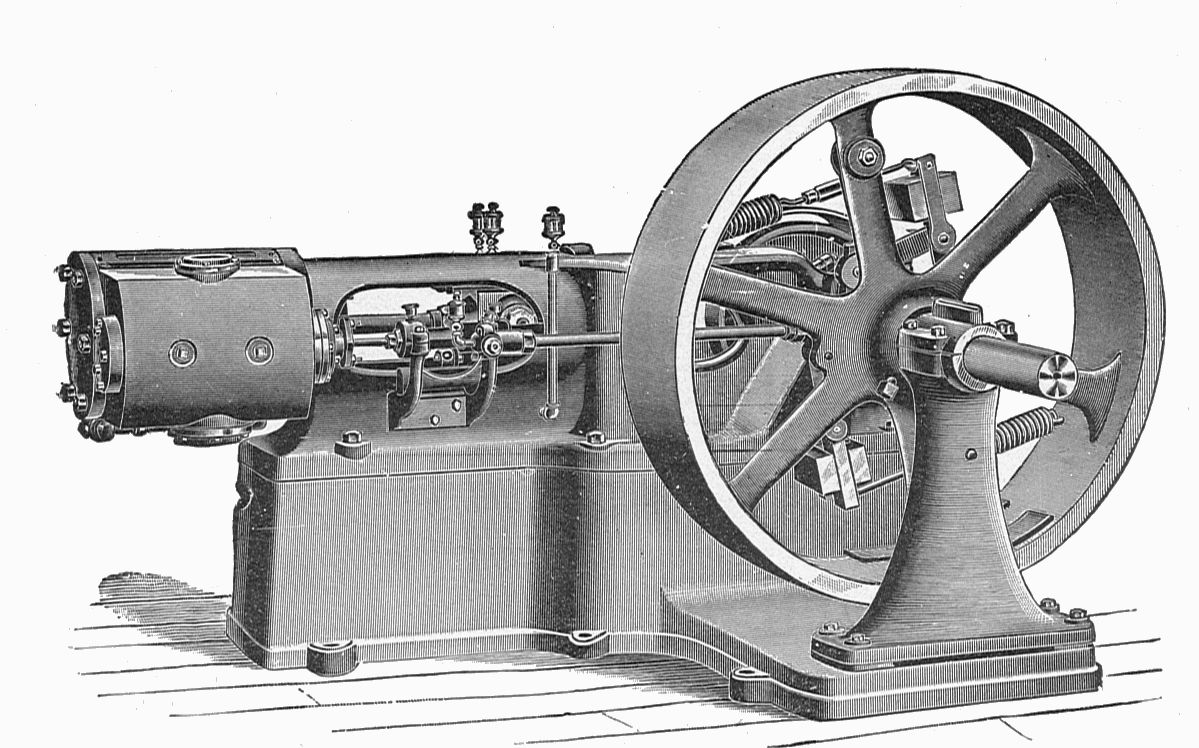
\includegraphics[width=0.5\textwidth]{sengine.jpg}};}
\end{frame}

\begin{frame}
 \frametitle{Ptolemy and the almagest}
 \begin{columns}
   \column{0.5\textwidth}\centering
     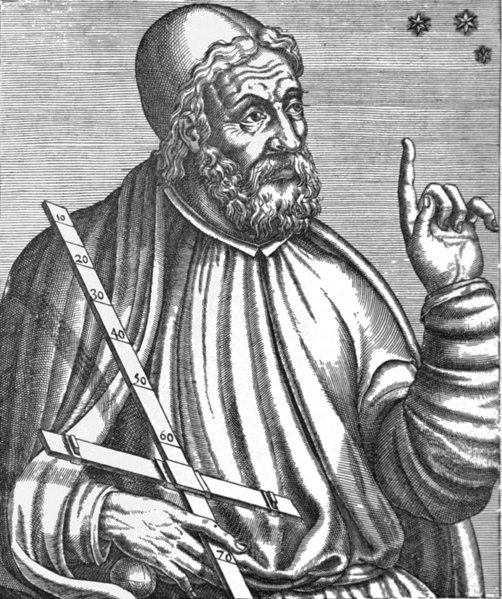
\includegraphics[height=0.7\columnwidth]{Ptolemy.png}
   \column{0.5\textwidth}\centering
     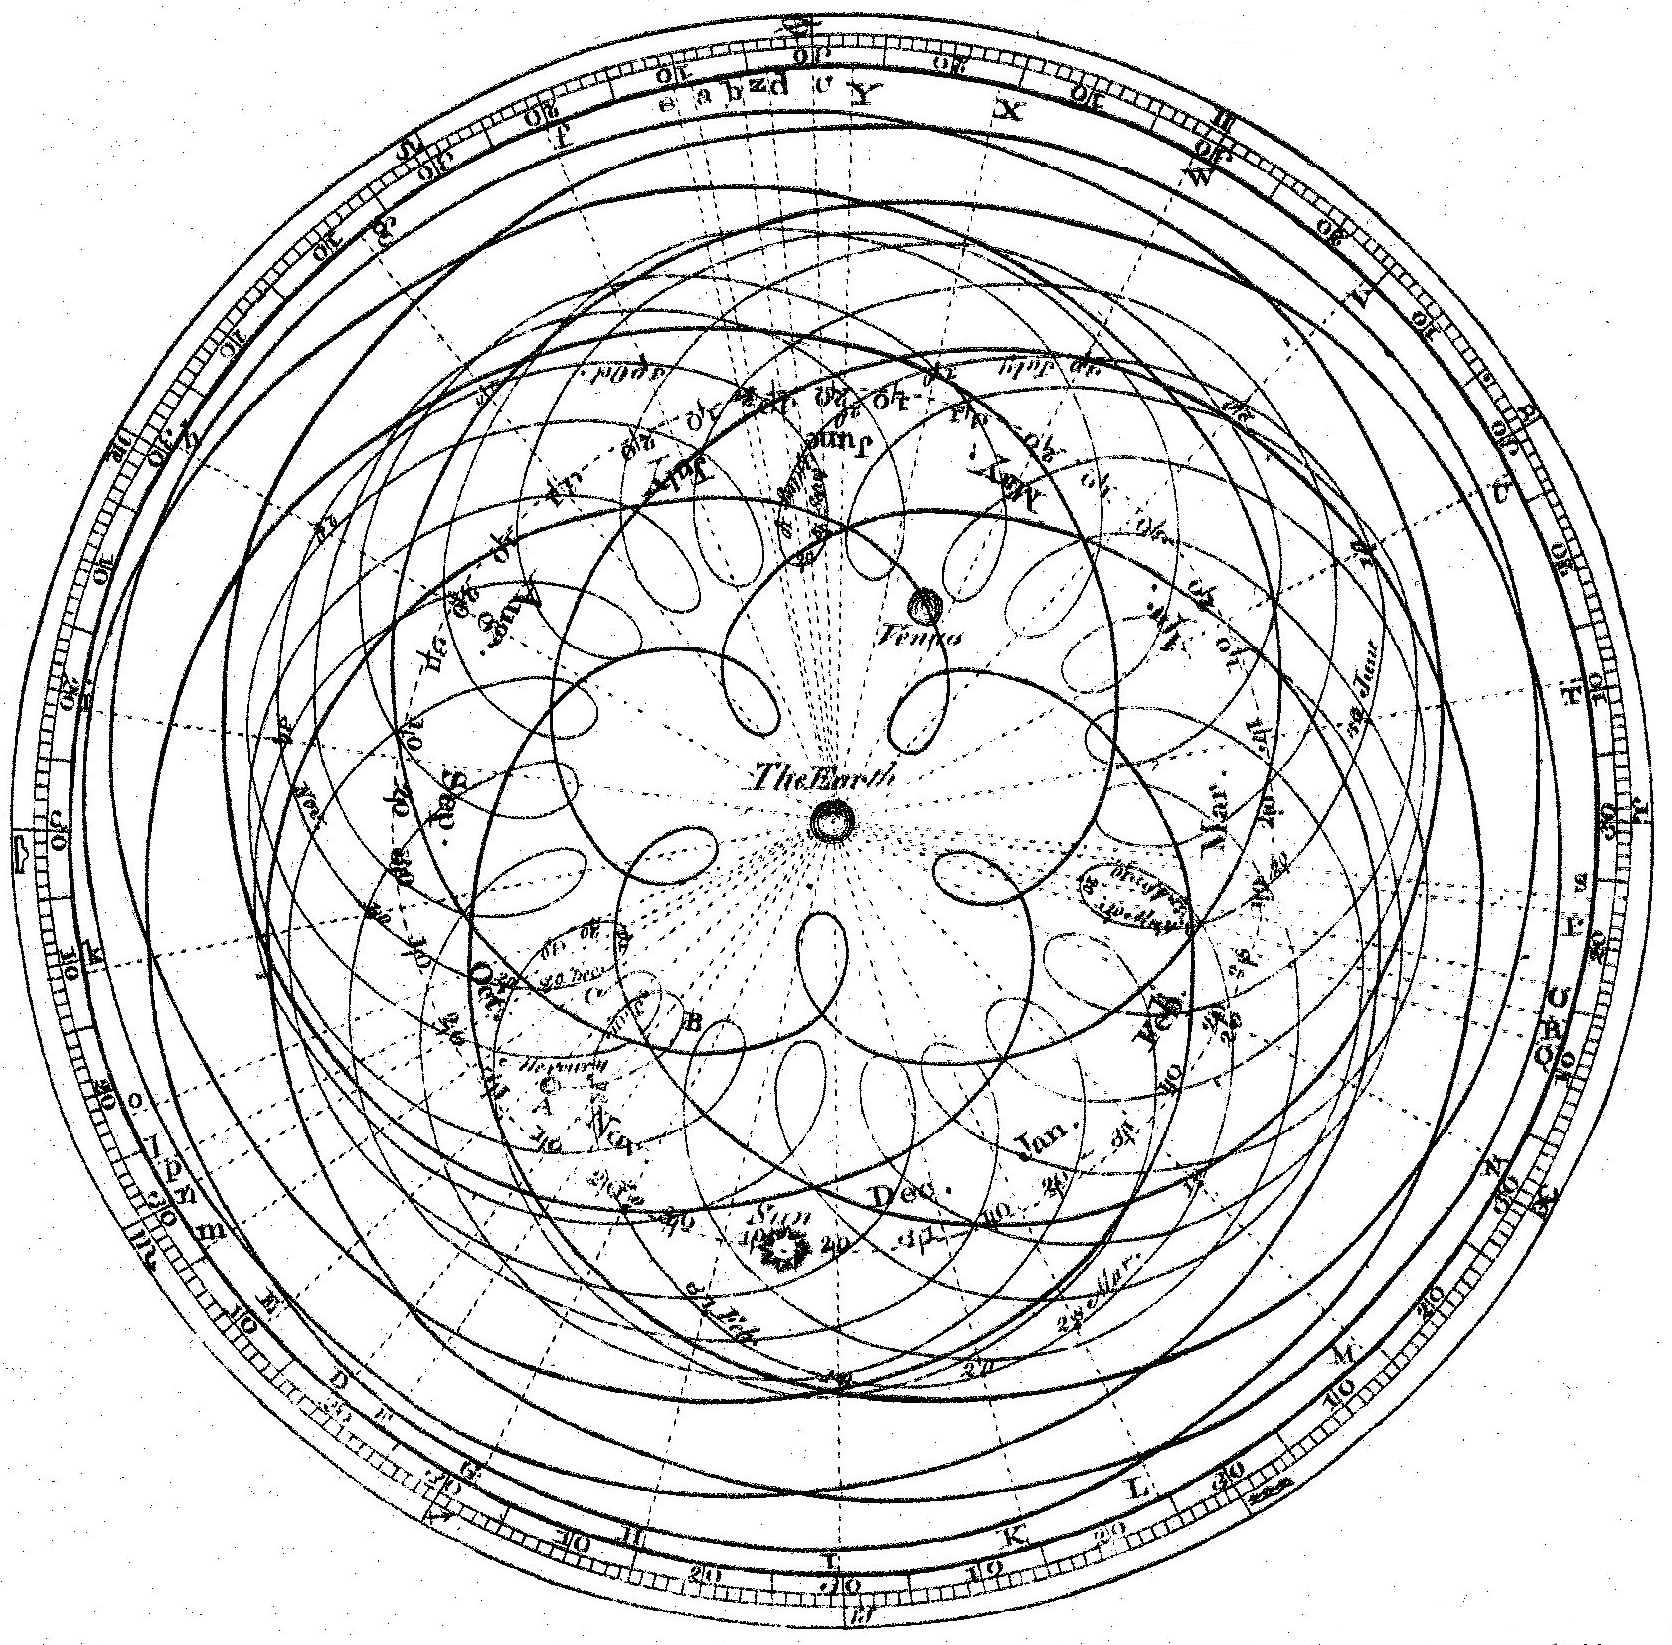
\includegraphics[width=0.8\columnwidth]{Cassini_apparent.png}   
 \end{columns} \vspace{1em}
 \tikz{\node[emphblock,text width=\textwidth]{
   ${\sim}150$ AD. Development of numerical approximations to describe the motions of the heavenly bodies with accuracy matching reality sufficiently.};}
\end{frame}
}

\begin{frame}
 \frametitle{Numerical Methods}
 \begin{itemize}
  \item Numerical analysis is concerned with obtaining approximate solutions to problems while maintaining reasonable bounds of error...
  \item ...because it is often impossible to obtain exact answers ...
  \item Numerical analysis makes use of algorithms to
approximate solutions
 \end{itemize}
\end{frame}

\begin{frame}
 \frametitle{Used in many fields... Including Chemical Engineering}
  \begin{itemize}
	  \item Description of reactors and separators (dynamic and steady state)
		\item Computational fluid dynamics
		\item Thermodynamic equations of state
		\item Optimizing process performance
		\item Design and synthesis of processes
		\item Regression of data, e.g. isotherms, kinetics, ...
 \end{itemize}
\end{frame}

\section{About this course}
\subsection{About}
\begin{frame}
  \frametitle{Course Schedule}
  \centering
  \begin{tabular}{cll}
  \hline
  Lecture  & Topic & Teacher \\ 
  \hline
  1 & Programming and algorithms (1) & IR \\ 
  2 & Programming and algorithms (2) & IR \\ 
  3 & Numerical errors & IR \\ 
  4 & Linear eqns: direct methods & IR\\ 
  5 & Linear eqns: iterative methods & IR \\ 
  6 & Interpolation + integration & IR \\ 
  7 & Non-linear equations (1) & MSA \\ 
  8 & Non-linear equations (2) & MSA\\ 
  9 & ODEs (1) & MSA \\
  10 & ODEs (2) & MSA \\ 
  11 & PDEs & MSA \\ 
  12 & Regression and Optimization & IR \\ 
  \hline
  \end{tabular} 
 \end{frame}

\begin{frame}
 \frametitle{Course Objectives}
 \begin{itemize}
  \item Gain experience with programming basics and algorithm design (Python, Excel)
  \item Understand the background of important numerical algorithms used in CEC 
  \item Recognize and solve (systems of) linear, non-linear and differential equations numerically
  \item Learn about numerical integration, interpolation, optimization
  \item Apply your skills to solve realistic assignments and small sample problems
 \end{itemize}
\end{frame}

\begin{frame}
 \frametitle{Prerequisites}
  The following courses should give you enough background knowledge to follow this course comfortably:
 \begin{itemize}
   \item Calculus
   \item Linear Algebra
   \item Some basic Python experience
     \begin{itemize}
      \item We will shortly cover some aspects on Python programming in the first lectures. Detailed documents and courses are provided on Canvas, for your own reference.     
    \end{itemize}
  \end{itemize}
  You will definitely need a laptop with Python and Excel installed!
\end{frame}

\begin{frame}
 \frametitle{Course Materials}
 \begin{itemize}
  \item Lecture slides (+ lecture recordings?)
  \item Python scripts
  \item Additional articles
  \item There are some useful books for those seeking more in-depth knowledge and alternative methods, not mandatory:
  \begin{itemize}
    \item Numerical recipes, W.H. Press et al.
    \item Numerical methods for chemical engineering, K.J. Beers
    \item Numerical methods for chemical engineers, A. Constantinides
    \item Python Crash Course, 3rd Edition, Eric Matthes
  \end{itemize}
 \end{itemize}
  \tikz{\node[emphblock,text width=\textwidth]{
    Look on Canvas for the slides, exercises, scripts, assignments and additional documentation on Python.
   };}
\end{frame}

\section{Assessments}
\subsection{Assessments}
{\nologo
\begin{frame}
 \frametitle{Assessment}
 \begin{block}{4 assignments}
  \begin{itemize}
    \item Each 20\% of the final result
    \item Done in groups of 2 persons, see Canvas$\,\to\,$People$\,\to\,$Project Groups
    \item Short report (template provided, Overleaf and Canvas)
    \item Assignment 1--3 graded through peer review
    \end{itemize}   
 \end{block}
 \pause
 \begin{block}{Final exam}
  \begin{itemize}
    \item Practical and theoretical questions, covering \emph{all topics}
    \item Exam taken on your own computer
    \item You can use the slides and modules documentation
    \item Sample exam will be released before Christmas
    \item Grade of the final exam needs to be at least a 5.0
  \end{itemize}   
 \end{block}
\end{frame}
}

\begin{frame}
  \frametitle{Assignment grading: peer assessment \& feedback (1)}
  \begin{itemize}
    \item Assignments are graded through supervised peer-assessment. After the deadline, each \emph{person} will grade 2 other assignments. Rubrics are available to maintain a consistent assessment among different groups. Criteria are:\hfill
      \begin{columns}
        \column{0.4\textwidth}
          \begin{itemize}
            \item Algorithm design
            \item Code quality
            \item Verification, validation and analysis
          \end{itemize}
        \column{0.4\textwidth}
          \begin{itemize}
            \item Visualisation
            \item Report
            \item Creativity
          \end{itemize}
      \end{columns}
    \item Review are done within 3 days (rubrics+written feedback to establish its validity). We assess the feedback quality by a multiplier (0.8-1.2).
    \item You can challenge one or more reviews by submitting a rebuttal;
    \item The final grade will be the averaged grade from the remaining peer-assessments (group), multiplied by the peer-review quality (individual), with a max. of 10.
    \item When statistics are poor ($\leq 2$ reviews), the assignment will be graded by the instructor, which discards all remaining peer-reviews.
  \end{itemize}
\end{frame}

\begin{frame}
\frametitle{Assignment grading: peer assessment \& feedback (2)}
\begin{itemize}
  \item Along with the rubrics, you will give each other specific comments for improvement: What are you impressed with; why did you score a certain criteria low; how to improve the code or  visuals, etc. Give at least 3 tips and 3 tops.
  \item Grades for an assignment are released only when proper assessment and feedback have been given.
  \item Rebuttals are turned in through an additional assignment. A rebuttal should convince us and provide evidence and in-depth argumentation why a particular review is flawed. We will evaluate the rebuttals and discard a peer-review if it is indeed disproportionate.
  \item We are getting help from teaching assistants to make the process go smoothly. I will show a possible solution after the deadline.
  \item Grading with rubrics: don't be afraid to use the full spectrum.
\end{itemize}
\end{frame}

\begin{frame}
  \frametitle{Peer assessment in the past}
  \begin{columns}
    \column{0.5\textwidth}\centering
      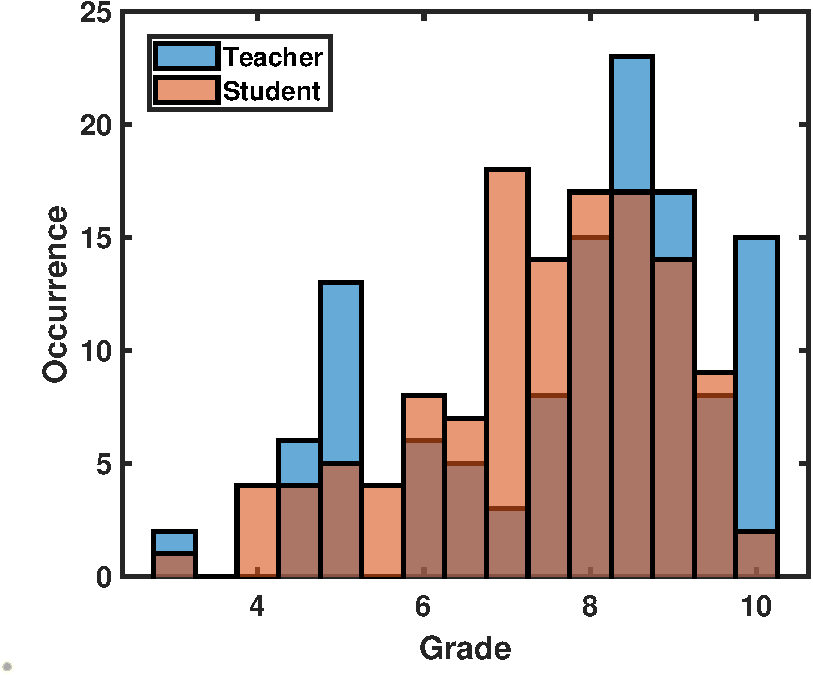
\includegraphics[height=0.8\columnwidth]{histogram-TS-crop}
    \column{0.5\textwidth}\centering
      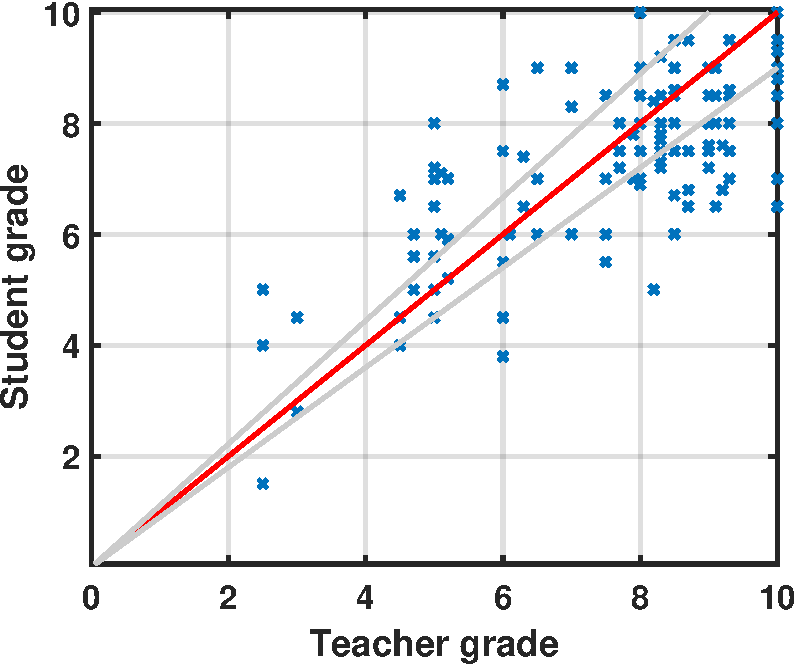
\includegraphics[width=0.8\columnwidth]{scatter}   
  \end{columns}
 \end{frame}

 \begin{frame}
  \frametitle{Peer assessment summary}
  Complete document can be read through Canvas, here's the summary:
  \begin{itemize}
    \item The assignment and report template are released along with the grading rubrics
    \item Canvas automatically performs a plagiarism check
    \item The lecturer will give a short overview of how the assignment could have been solved (point of reference)
    \item Students have 3 days for double-blind peer assessment
    \item Students have the opportunity to challenge their reviewers (rebuttal)
    \item Lecturers and TAs will check the review quality, as well as the reports that have very low or very high marks or large deviations among reviews coarsely. I will provide a full correction when no suitable peer-reviews have been done.
    \item If a student fails to produce a good, timely peer-review, their grade for the assignment will be marked NA.
  \end{itemize}
 \end{frame}
%
\begin{frame}
 \frametitle{Assignment handout and deadlines}
     Hand-in your assignments via Canvas
    \begin{itemize}
      \item Deadlines are given on Canvas as well
      \item Deliver the report in PDF format
      \item Send along the scripts + necessities in a .zip
      \item Use your student ID instead of your name for identification purposes
      \item Be aware that a .docx stores the original author name as metadata.
    \end{itemize}
\end{frame}


\section{Finally...}
\subsection{Information}
{\nologo
\begin{frame}
  \frametitle{Course Philosophy}
 \begin{itemize}
  \item This is a hard course! It will take a lot of hours, especially if you have no coding experience.
  \item We are here to help you. To have nice discussions, to show alternative ways, etc. Clarify language subtleties, or suggestions. Not to give away the answers.
  \item We encourage research and independent learning. It comes down to paying attention, repetition of the concepts, and practice practice practice! 
  \item We try to make the lectures interactive, working on examples and creating scripts as we go. It is advised that you work along with us to get the most out of this course!
  \item It is ok to discuss the general approach to solving the problem, or to get a hint, or several hints, if you get stuck while solving a problem, but work out the details of the solution in your own group.
  \item It is {\textbf{not ok}} to take someone else's solution (or an AI/LLMs) and present it as your own work.
  \item Take regular breaks! Better 6 times per hour a short break than 1 time per hour a long break. Use keyboard shortcuts, or a mouse if you must. Set up screen brightness to a pleasant value. Stretch.
\end{itemize}
\end{frame}
}

\begin{frame}
 \frametitle{Contact information}
 \begin{block}{Ivo Roghair}
  \begin{itemize}
%    \item Contact via Canvas is preferred!
   \item E-mail: \href{mailto:i.roghair@tue.nl}{i.roghair@tue.nl}
   \item Office: STW 0.37
   \end{itemize} 
 \end{block}
 \vspace{1em}
  \begin{block}{Martin van Sint Annaland}
  \begin{itemize}
   \item E-mail: \href{mailto:m.v.sintannaland@tue.nl}{m.v.sintannaland@tue.nl}
   \item Office: STW 0.39 
   \end{itemize} 
 \end{block}
\end{frame}

% \begin{frame}
%  \frametitle{Some last remarks}
%   \begin{itemize}
%   \item Tell us if something is not clear.
%   \item We try to make the lectures interactive, working on examples and creating scripts as we go. It is advised that you work along with us to get the most out of this course!
%   \item The exercises are meant to provide a jump start towards the assignments.
%   \item We will always answer questions on the exercises. We may didactically answer questions on the assignments.
%   \item During the lectures/tutorials we first and foremost work on the exercises. If they are done, you can work on the assignment if you want.
%   \end{itemize} 
% \end{frame}

\begin{frame}
 \frametitle{Some Acknowledgements}
 \centering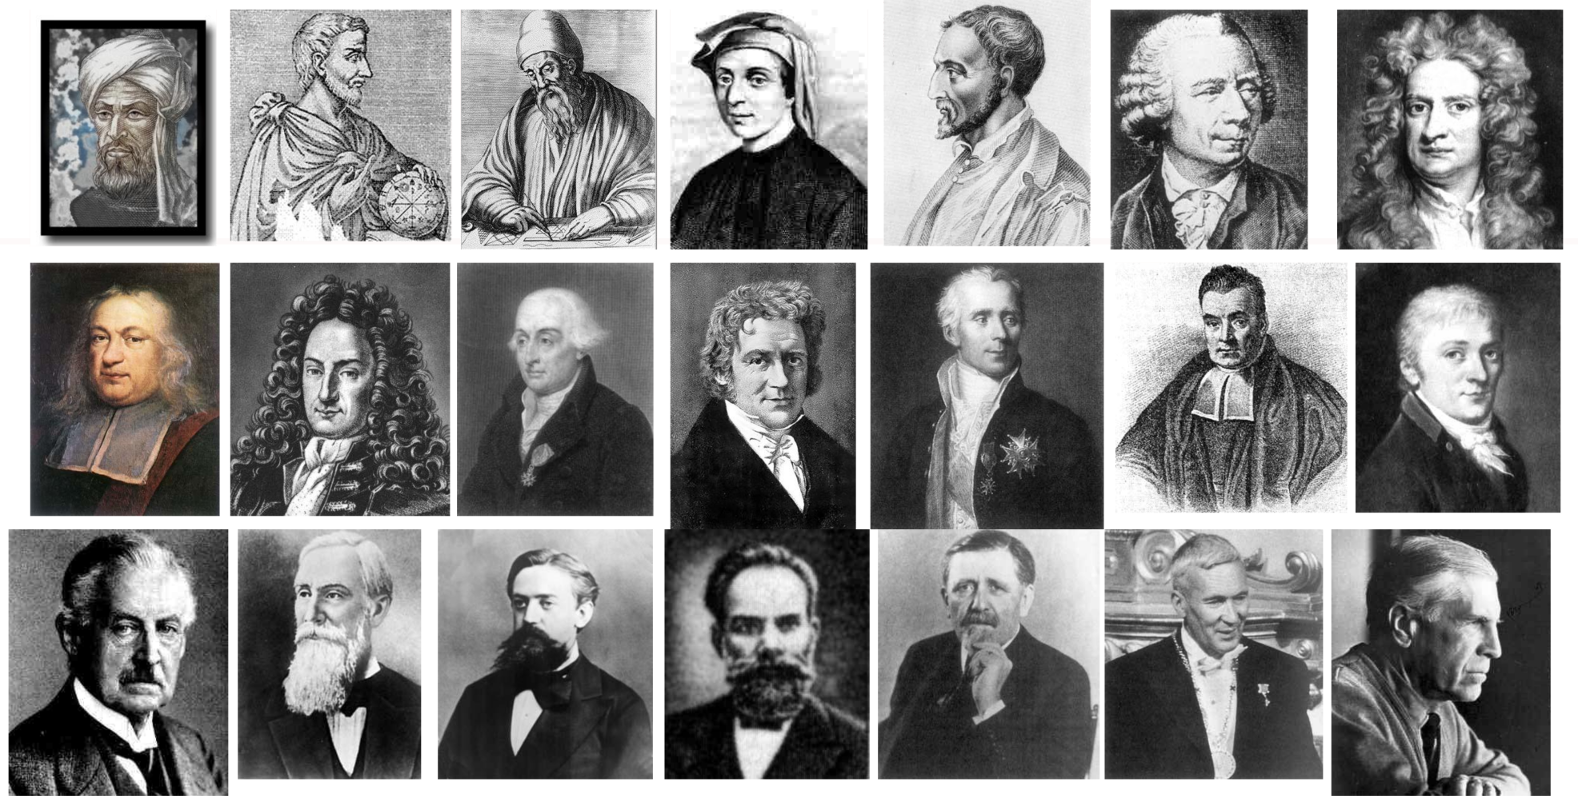
\includegraphics[width=\textwidth]{ack.png}
\end{frame}

\begin{frame}
 \frametitle{Some Real Acknowledgements}
 For inspiration, examples and exercises:
 \begin{itemize}
  \item To Roel Verstappen of Groningen University
  \item To Johan Hult of Cambridge University
  \item To Edwin Zondervan of University of Twente
  \item To edX: MITx course  "Introduction to Computer Science and Programming Using Python"
 \end{itemize}
\end{frame}
% \end{document}


% References
% http://ocw.mit.edu/courses/electrical-engineering-and-computer-science/6-00sc-introduction-to-computer-science-and-programming-spring-2011/unit-1/lecture-1-introduction-to-6.00/
% http://www.greenteapress.com/thinkpython/html/thinkpython002.html
% https://www.youtube.com/channel/UCLMQ21H2ad95faYG3yGCwYA
%http://stackoverflow.com/questions/4227145/in-matlab-are-variables-really-double-precision-by-default
%http://www.exploringbinary.com/why-0-point-1-does-not-exist-in-floating-point/



\title{Matlab and Programming 1}
\subtitle{Programming basics and algorithms}
\lecture{Programming 1}{programming1}
\part{Python programming I}
\section{Introduction}
\subsection*{General}
\begin{frame}[label=contents_prog1]
  \frametitle{Today's outline}
  \mode<beamer>{
    \only<1>{
      \begin{columns}
        \column{0.5\textwidth}
          \tableofcontents[sections={1-3}]
        \column{0.5\textwidth}
          \tableofcontents[sections={4-8}]
      \end{columns}}
  }
  \only<2>{
    \begin{columns}
      \column{0.5\textwidth}
        \tableofcontents[sections={1-3},currentsection]
      \column{0.5\textwidth}
        \tableofcontents[sections={4-8},currentsection]
    \end{columns}
    }
\end{frame}

\subsection{General programming}
\begin{frame}
  \frametitle{Why should you learn something about programming?}
  \begin{itemize}[<+->]
    \item Scientific techniques depend in an increasing fashion upon computer programs and simulation methods
    \item Knowledge of programming allows you to automate routine tasks 
    \item Ability to understand algorithms by inspection of the code 
    \item Learn to think by dissecting a problem into smaller, easier to solve, parts 
  \end{itemize}\vskip2em
  \begin{columns}
    \column<1->{0.23\textwidth}
    \tikz\node[circle,draw,very thick,maincolor,
    text=white,minimum size=\columnwidth,
    path picture={
    \node at (path picture bounding box.center){
      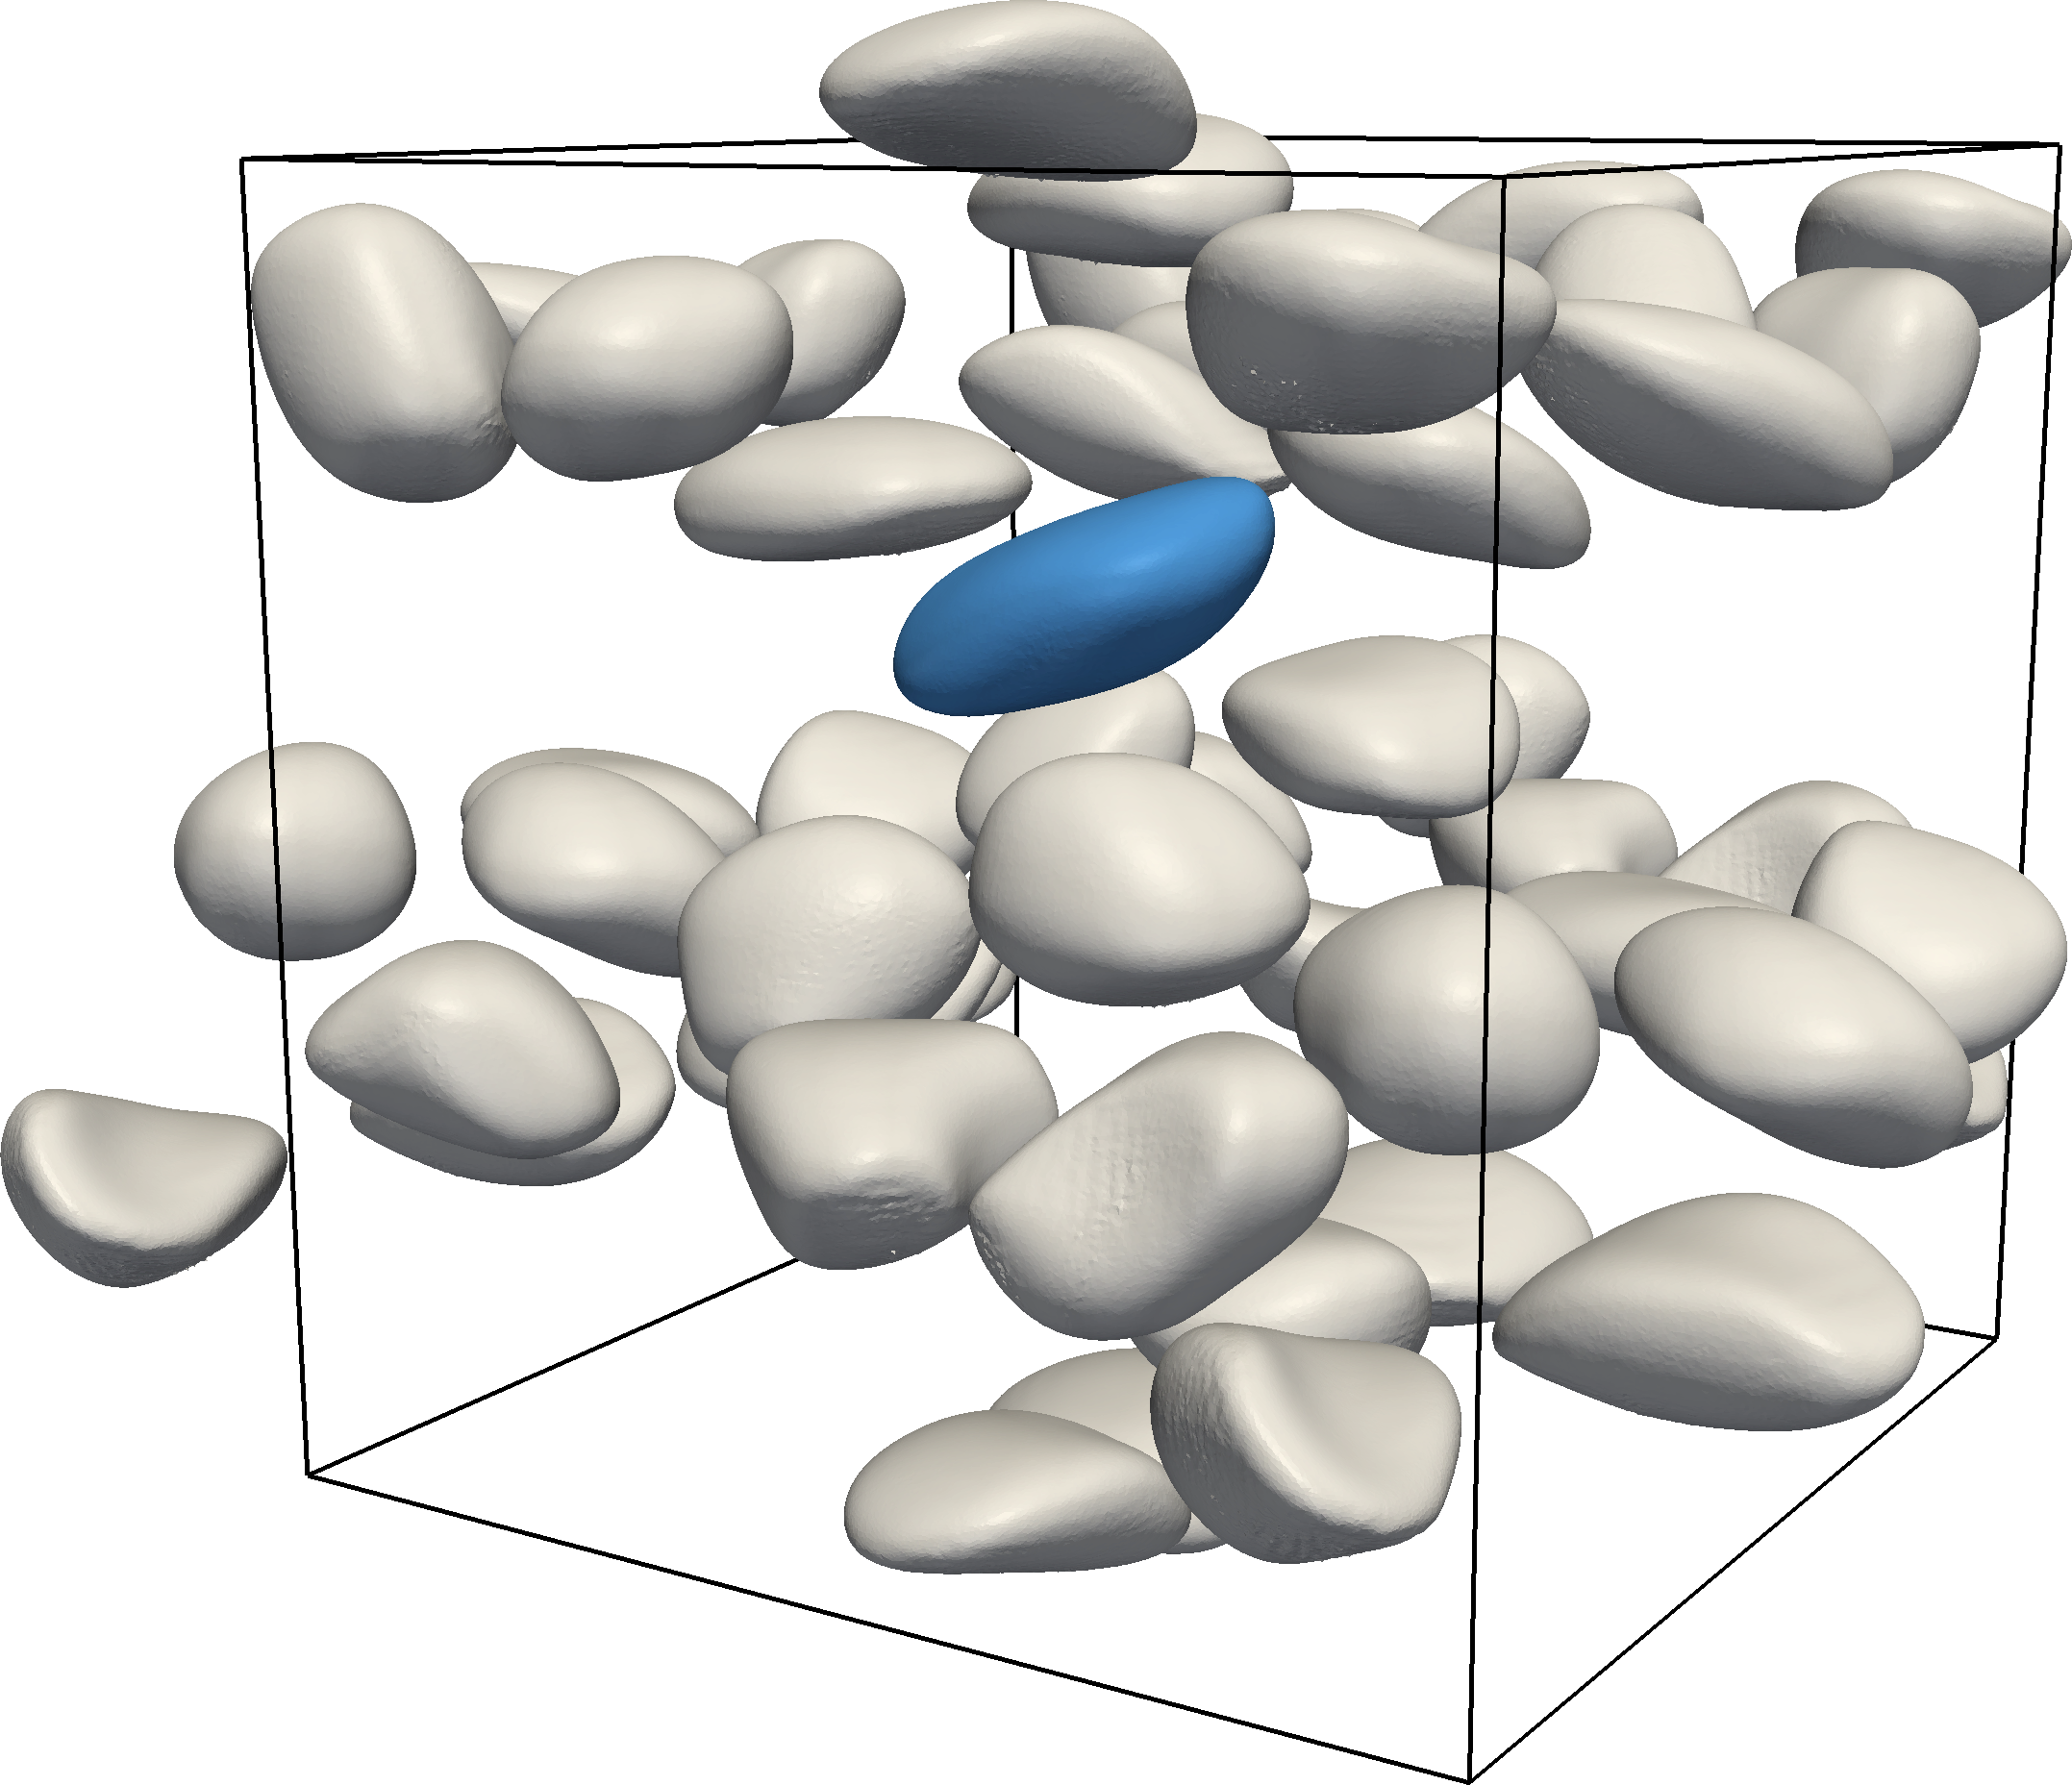
\includegraphics[width=\columnwidth]{sim1.png}
      };
      }]{};
  \column<2->{0.23\textwidth}
  \tikz\node[circle,draw,very thick,maincolor,
  text=white,minimum size=\columnwidth,
  path picture={
    \node at (path picture bounding box.center){
                   
\includegraphics[width=1.1\columnwidth]{automate.jpg}
                   };
                   }]{};
                   \column<3->{0.23\textwidth}
                   \tikz\node[circle,draw,very thick,maincolor,
                   text=white,minimum size=\columnwidth,
                   path picture={
               \node at (path picture bounding box.center){
                 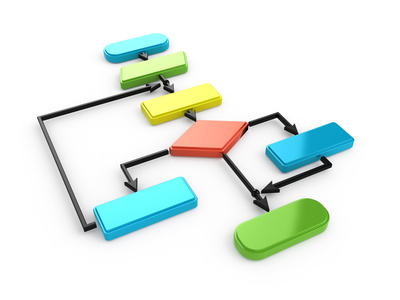
\includegraphics[width=1.2\columnwidth]{algorithm.jpg}
                 };
                 }]{};
                 \column<4>{0.23\textwidth}
                 \tikz\node[circle,draw,very thick,maincolor,
                 text=white,minimum size=\columnwidth,
                 path picture={
                   \node at (path picture bounding box.center){
                     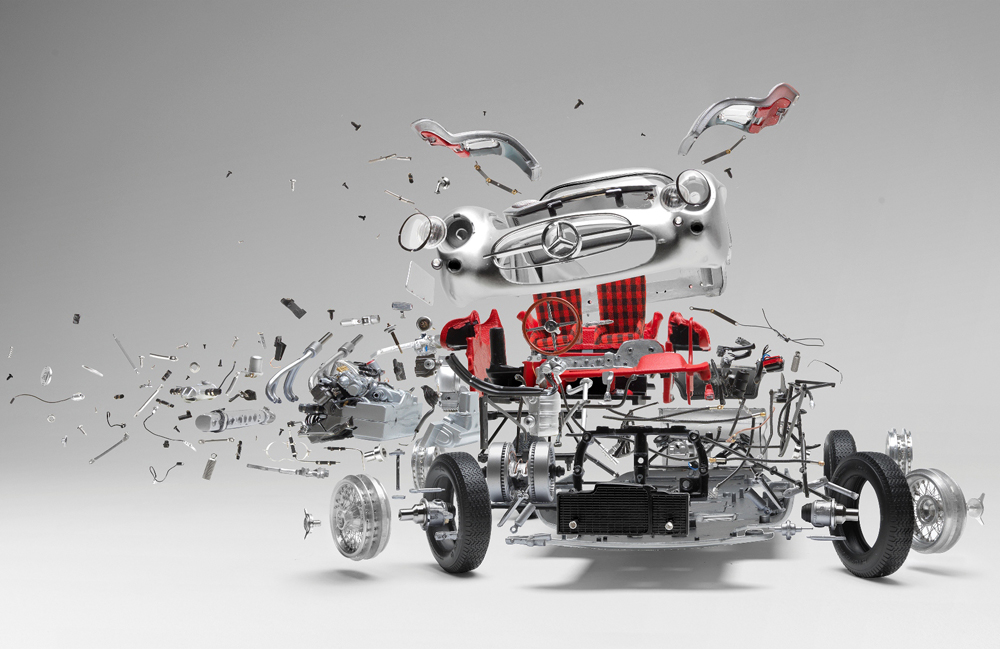
\includegraphics[width=1.5\columnwidth]{dissect.jpg}
                     };
                     }]{};
                    \end{columns}
                  \end{frame}
                  
                  \begin{frame}
                \frametitle{Introduction to programming}
                \begin{block}{What is a program?}
                  \emph{A program is a sequence of instructions that is written to perform a certain task on a computer.} % SOURCE http://www.greenteapress.com/thinkpython/html/thinkpython002.html
                \end{block}
                \begin{itemize}
                  \item The computation might be something mathematical, a symbolic operation, image analysis, etc.%such as solving a system of equations or finding the roots of a polynomial
                  % \item It can also be a symbolic computation, such as searching and replacing text in a document 
                  % \item A program may even be used to compile another program
                  % \item A program consists of one or more \emph{algorithms}
                \end{itemize}
                \begin{block}{Program layout}
  \begin{enumerate}
    \item Input (Get the radius of a circle)
    \item Operations (Compute and store the area of the circle)
    \item Output (Print the area to the screen)
  \end{enumerate}
\end{block}
\end{frame}

\begin{frame}
  \frametitle{Versatility of Python}
  \centering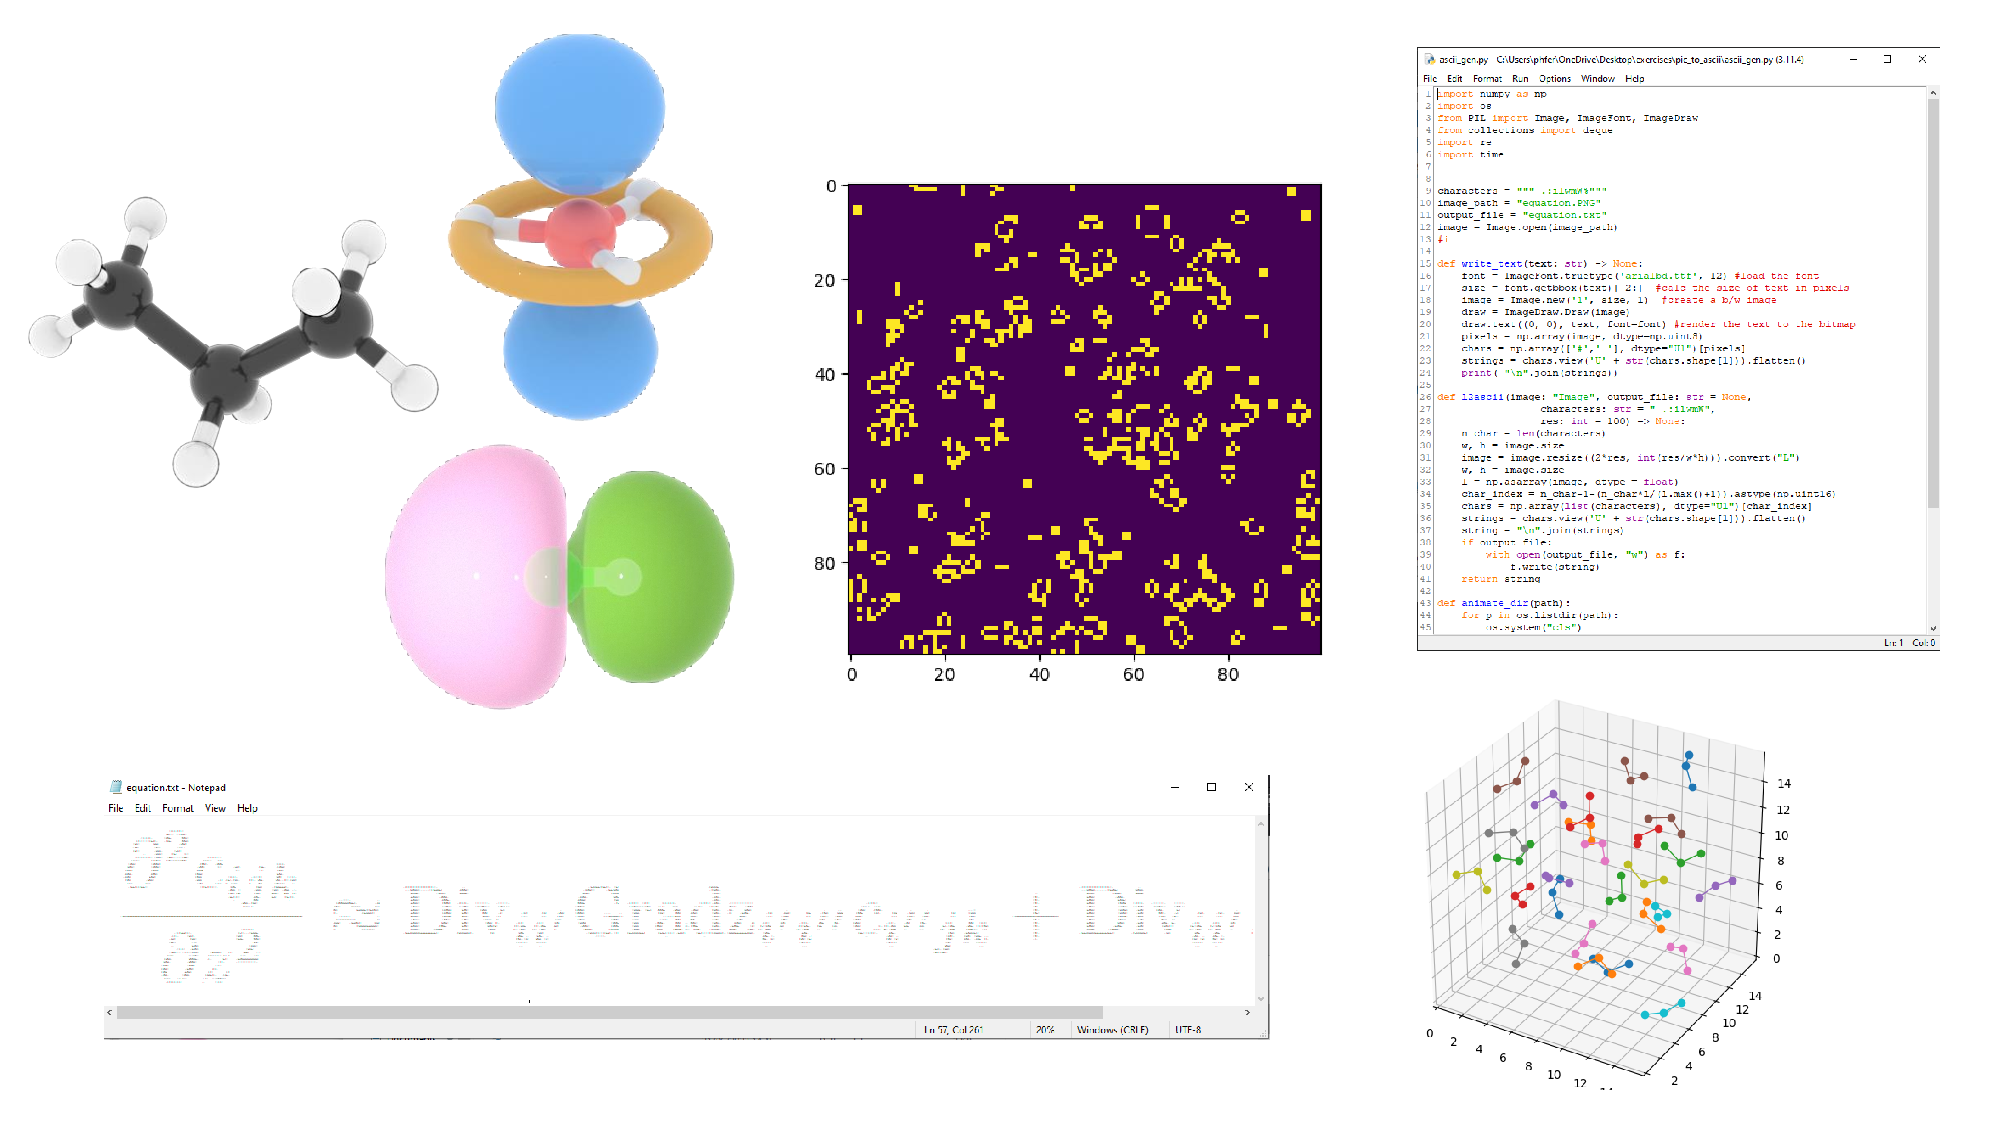
\includegraphics[width=0.9\textwidth]{python_versatility.pdf}
\end{frame}

\begin{frame}
  \frametitle{Versatility of Python: ODE solver}
  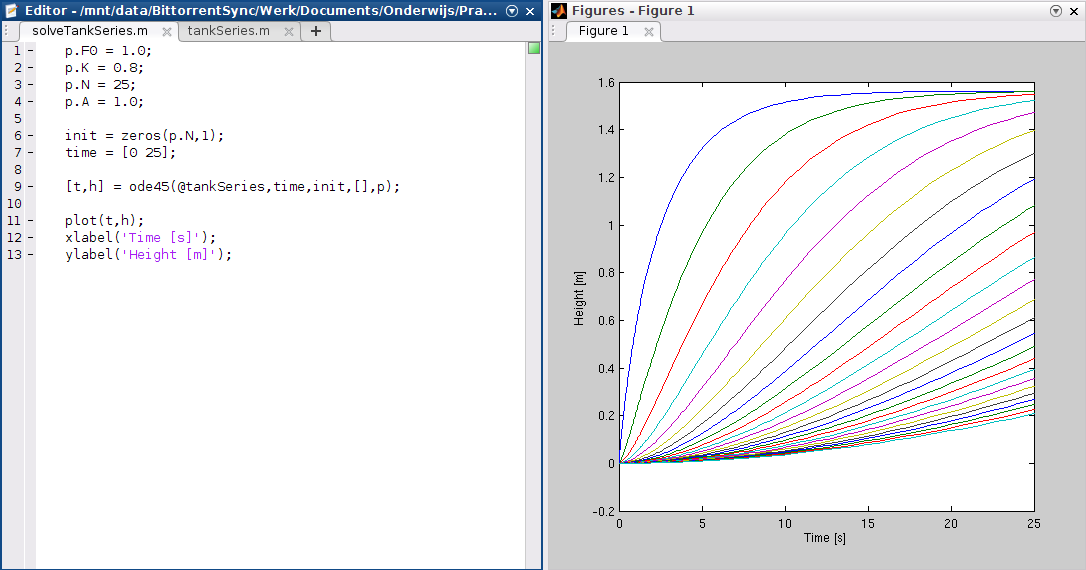
\includegraphics[width=\textwidth]{odesol.png}
\end{frame}

\begin{frame}[fragile]
  \frametitle{Versatility of Python: Image analysis}
  \begin{columns}
    \column{0.5\textwidth}
    \begin{lstlisting}
# Importing necessary libraries
import numpy as np
from scipy import ndimage
from PIL.Image import fromarray
from skimage import io, color, feature, measure

# Loading and processing image 
I = io.imread('bub0.png')
BW = color.rgb2gray(I)
E = feature.canny(BW) 
F = ndimage.binary_fill_holes(E)

# Show final image
fromarray(F).show()
    \end{lstlisting}  
    \column{0.5\textwidth}
    \vfill
    \includegraphics<1>[width=\columnwidth]{bub1.png}
    \includegraphics<2>[width=\columnwidth]{bub2.png}
    \includegraphics<3>[width=\columnwidth]{bub3.png}
    \includegraphics<4>[width=\columnwidth]{bub4.png}
  \end{columns}
\end{frame}

{\nologo
\begin{frame}
  \frametitle{Versatility of Python: Curve fitting}
  \centering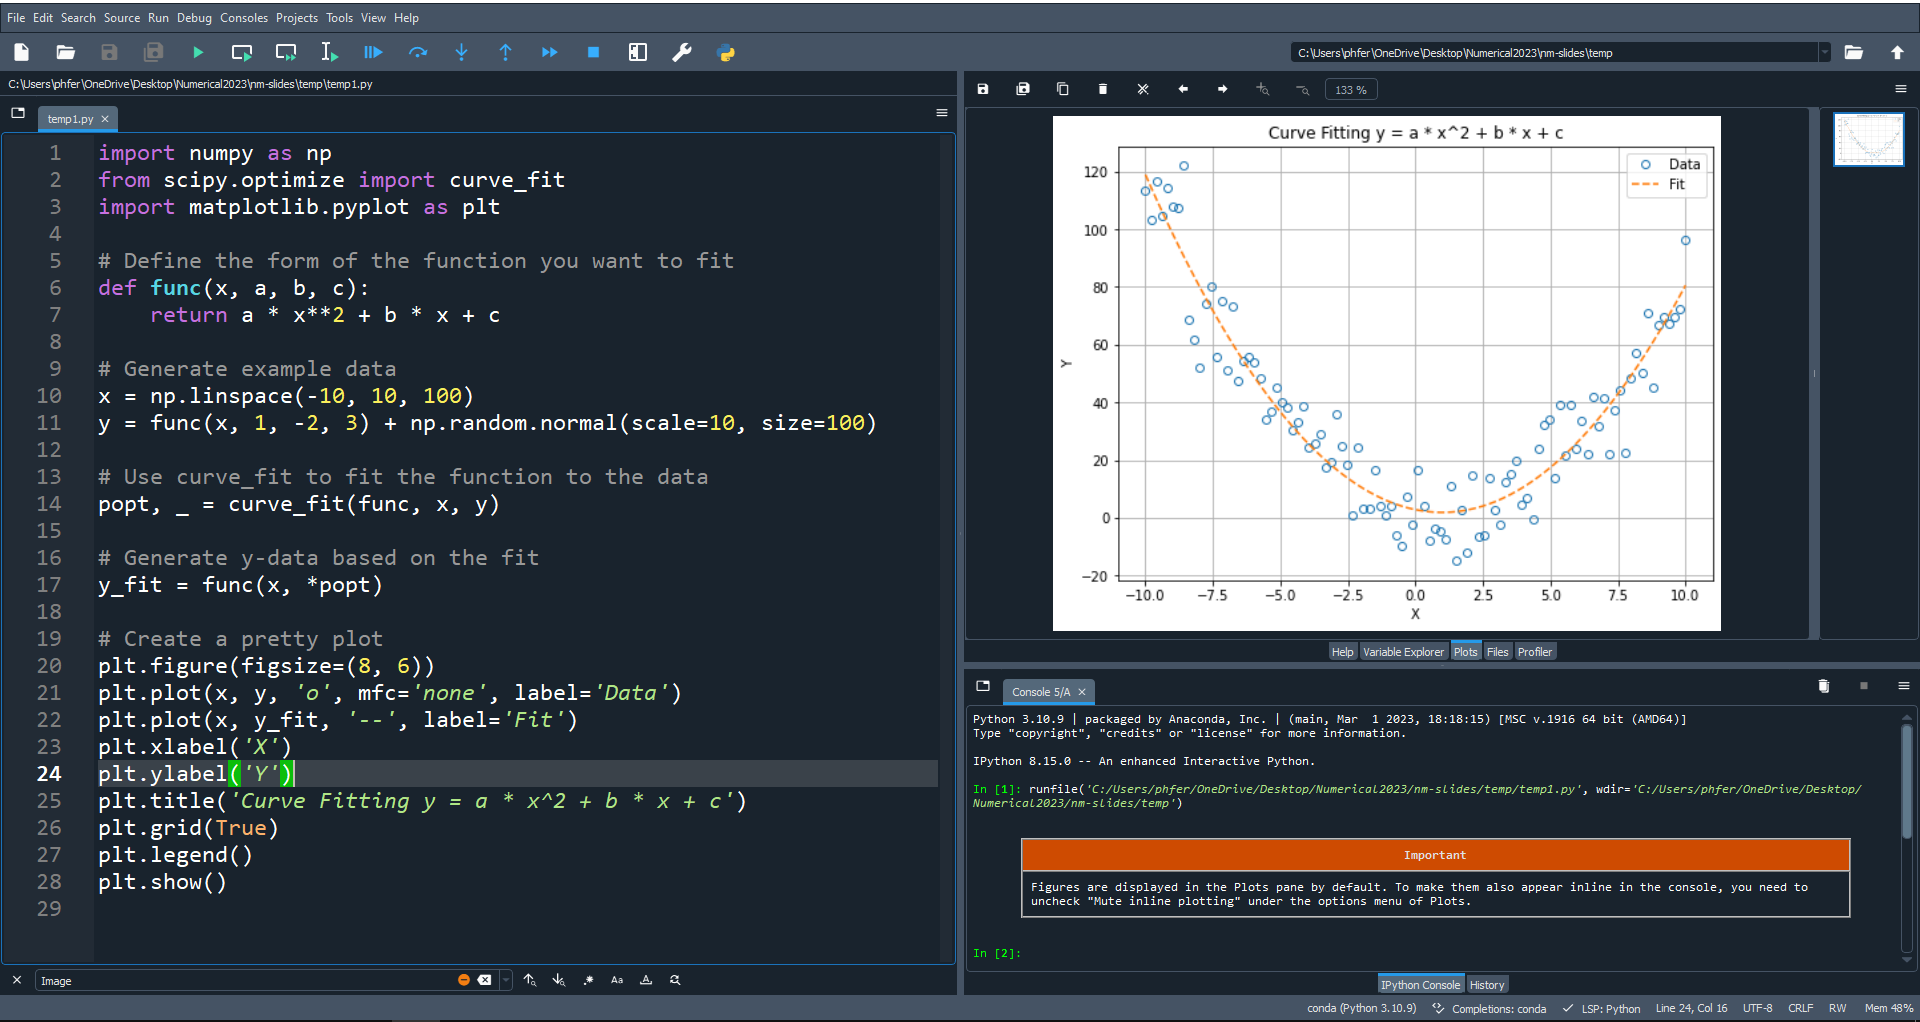
\includegraphics[width=\textwidth]{cftool.png}
\end{frame}
}

\subsection{First steps}
\begin{frame}[fragile]
  \frametitle{Getting started}
  \begin{itemize}
    \item Start the Python REPL (read–eval–print loop) by running \lstinline|python| or \lstinline|ipython|
    \item Enter the following commands on the command line. Evaluate the output.
  \end{itemize}
  \pause
  \begin{columns}
    \column{0.75\textwidth} 
      \begin{lstlisting}[numbers=none]
>>> 2 + 3        # Some simple calculations
>>> 2 * 3
>>> 2 * 3**2     # Powers are done using ** (*@ \pause @*)
>>> a = 2        # Storing values into the workspace
>>> b = 3
>>> c = (2 * 3)**2  # Parentheses set priority
>>> 8 / a - b (*@ \pause @*)
>>> import math  # Mathematical functions can be used 
>>> math.sin(a)  
>>> math.sin(0.5 * math.pi)  # math.pi is an internal Python variable
>>> import cmath  # for working with complex numbers
>>> cmath.sqrt(-1)  # ... as are imaginary numbers    
      \end{lstlisting}\pause
    \column{0.25\textwidth} 
      \begin{lstlisting}[style=PyOutput,numbers=none]
5
6
18



1.0

0.9092974268256817
1.0

1j
      \end{lstlisting}
  \end{columns}
\end{frame}

\begin{frame}[fragile]
  \frametitle{Printing and formatting results}
  You can control the formatting of variables in string literals using various methods - we recommend f-strings. Note that formatting only changes how numbers are \emph{displayed}, not the underlying representation.

  \begin{lstlisting}[language=Python,numbers=none]
>>> a = 19/4
>>> print("Few digits {:.2f}".format(a)) # 2 decimal places
>>> print("Many digits {:.10f}".format(a)) # 10 decimal places
>>> 
>>> b = 22/7
>>> i = 13
>>> print("Almost pi: %1.4f" % b)
>>> print("i = %d, a = %1.4f and b = %1.8f" % (i,a,b))
>>>
>>> # Using f-strings (Python 3.6+)
>>> c = (21)**0.5 # sqrt of 21
>>> print(f"{c:.10f}") # Float with 10 decimal places
>>> mystr = f"{c:.2e}" # Scientific notation with 2 decimal places in a string object
>>> print(mystr) # Print the string object
>>> print(f"{b=}") # Use = to print variable name and value
>>> print(f"{b=:_^15.2}") # Adjust spacing and spacer character
  \end{lstlisting}
\end{frame}
 
 {\nologo
 \begin{frame}[fragile]
  \frametitle{A few helpful things}
  \begin{itemize}[<+->]
    \item Using the \keystroke{$\uparrow$} and \keystroke{$\downarrow$} keys, you can cycle through recent commands
    \item Typing part of a command and pressing \keystroke{Tab} completes the command and lists the possibilities
    \item If a computation takes too long, you can press \keystroke{Ctrl}+\keystroke{C} to stop the program and return to the command line. Stored variables may contain incomplete results.
    \item Sequences of commands (programs, scripts) are contained as py-files, plain text files with the \lstinline$.py$ extension.
    \item Python scripts can also be contained in jupyter notebooks, which have extension \lstinline$.ipynb$.
    \item Such py-files must be in the \emph{current working directory} or in the Python \emph{path}, the locations where Python searches for a command. If you try to run a script that is not in the path, Python will throw an Exception/Error.
    \item Anything following a \lstinline$#$ symbol is regarded as a comment
    \item There are several keyboard shortcuts (vary with text editor) that will make coding much more efficient.
  \end{itemize}
\end{frame}
}

\begin{frame}[fragile]
  \frametitle{Scripts, notebooks and REPL}
  \begin{itemize}
    \item The REPL, indicated by the \lstinline|>>>| prompt, has the advantage of immediate result after typing a command.
    \item Larger programs are better written in separate files; either Jupyter notebooks (.ipynb files) or plain script files (.py files).
    \item Defining functions in such files will put them in the \emph{scope}, but will not run them until they are actually called.
    \item The snippets in these slides will continue to use the REPL for single-line commands, and move towards scripts when larger functions are being constructed.
  \end{itemize}
\end{frame}

\subsection{Further reading}
\begin{frame}[fragile]
\frametitle{Python help, documentation, resources}
\begin{itemize}[<+->]
  \item Refer to the Python documentation at \href{https://docs.python.org/3/}{Official documentation}.
  \begin{itemize}
    \item Try for instance: \lstinline$help(print)$ or \lstinline$help(help)$.
  \end{itemize}
  \item We supply a number of basic practice/reference modules: Python Crash Course.
  \item \href{https://tue.on.worldcat.org/oclc/1346554335}{Python Crash Course, 3rd Edition \faExternalLink} by Eric Matthes
  \item \href{https://tue.on.worldcat.org/oclc/1023864062}{A Whirlwind Tour of Python \faExternalLink} by Jake Vanderplas
  \item \href{https://tue.on.worldcat.org/oclc/1164494156}{Introduction to Scientific Programming with Python \faExternalLink} by Joakim Sundnes
  \item \href{https://pythonnumericalmethods.berkeley.edu/notebooks/Index.html}{Python Programming And Numerical Methods: A Guide For Engineers And Scientists \faExternalLink} by Kong, Siauw and Bayen
  \item Search the web, Reddit, YouTube, etc.
\end{itemize}
\end{frame}

\section{Data structures}
\subsection{Data types}
\againframe<2>{contents_prog1}
\begin{frame}
 \frametitle{Terminology}
 \begin{description}
  \item[Variable] Piece of data stored in the computer memory, to be referenced and/or manipulated
  \item[Function] Piece of code that performs a certain operation/sequence of operations on given input
  \item[Operators] Mathematical operators (e.g. \lstinline$ + - *$ or \lstinline$/$), relational (e.g. \lstinline$< >$or \lstinline$==$, and logical operators (\lstinline$and$, \lstinline$or$)
  \item[Script] Piece of code that performs a certain sequence of operations without specified input/output
  \item[Expression] A command that combines variables, functions, operators and/or values to produce a result.
 \end{description}
\end{frame}

\begin{frame}[fragile]
 \frametitle{Variables in Python}
  \begin{itemize}
    \item Python stores variables in the \emph{namespace}\pause
    \item You should recognize the difference between the \emph{identifier} of a variable (its name, e.g. \lstinline$x$, \lstinline$setpoint_p$), and the data that it actually stores (e.g. 0.5)\pause
    \item Python also defines a number of functions by default, e.g. \lstinline$min$, \lstinline$max$ or \lstinline$sum$.
    \begin{itemize}
      \item A list of built-in methods is given by \lstinline$dir(__builtins__)$
    \end{itemize}
    \pause
    \item You can assign a variable by the \lstinline$=$ sign:
   \begin{lstlisting}[language=Python, numbers=none]
>>> x = 4*3
>>> x
12
   \end{lstlisting}\pause
   \item If you don't assign a variable, it will be stored in \lstinline$_$
   \item In most text editors, all variables are cleared automatically before the next execution. 
 \end{itemize}
\end{frame}

\begin{frame}[fragile]
  \frametitle{Datatypes and variables}
  Python uses different types of variables:
      \begin{longtable}{l!{\vrule}l}
       Datatype        & Example \\ \hline
       \lstinline$str$    & \lstinline$'Wednesday'$ \\
       \lstinline$int$    & \lstinline$15$ \\
       \lstinline$float$  & \lstinline$0.15$ \\
       \lstinline$list$   & \lstinline$[0.0, 0.1, 0.2, 'Hello', ['Another','List']]$ \\
       \lstinline$dict$   & \lstinline${'name': 'word', "n": 2}$ \\
       \lstinline$bool$   & \lstinline$False$ \\
       \lstinline$tuple$  & \lstinline$(True, False)$ \\
     \end{longtable}
     \pause
     Everything in Python is an object. You can use the \lstinline$dir()$ function to query the possible methods on an object of a datatype (e.g. \lstinline$(dir(list))$, \lstinline$dir(28)$ or \lstinline$dir("Yes!")$).
 \end{frame}

 %% LISTS SECTION
\subsection{Lists}
\begin{frame}[fragile]
  \frametitle{Lists in Python (1)}
  \begin{itemize}
    \item Lists are containers of collections of objects
    \item A list is initialized using square brackets with comma-separated elements
    \begin{lstlisting}[language=Python,numbers=none]
>>> brands = ['Audi', 'Toyota', 'Honda', 'Ford', 'Tesla']
    \end{lstlisting}
    \item Lists can contain and mix any object type, even other lists:
    \begin{lstlisting}[language=Python,numbers=none]
>>> another_list = [0.0, 0.1, 0.2, 'Hello', brands]
>>> print(another_list)
    \end{lstlisting}
    \begin{lstlisting}[style=PyOutput]
[0.0, 0.1, 0.2, 'Hello', ['Audi', 'Toyota', 'Honda', 'Ford', 'Tesla']]
    \end{lstlisting}
    \item Access (i.e., read) an entry in a list. Note that indexing starts at 0:
    \begin{lstlisting}[language=Python,numbers=none]
>>> print(another_list[0],another_list[3])
    \end{lstlisting}
    \begin{lstlisting}[style=PyOutput]
0.0 Hello
    \end{lstlisting}
  \end{itemize}
 \end{frame}
 
 \begin{frame}[fragile]
   \frametitle{Lists in Python (2)}
   \begin{itemize}
    \item Manipulate the value of an entry goes likewise:
    \begin{lstlisting}[language=Python,numbers=none]
>>> another_list[3] = 'Bye' # Becomes: [0.0, 0.1, 0.2, 'Bye', ['Audi', ...]]
    \end{lstlisting}
    \item Slicing is used to retrieve multiple elements:
    \begin{lstlisting}[language=Python,numbers=none]
>>> another_list[1:4] # This will give the elements from index 1 to index 3
    \end{lstlisting}
    \begin{lstlisting}[style=PyOutput]
[0.1, 0.2, 'Bye']
    \end{lstlisting}
    \item Lists can be unpacked into individual variables:
    \begin{lstlisting}[language=Python,numbers=none]
>>> a,b,c,d,e = brands
>>> print(f"The first list element was {a}, then {b}, {c}, {d} and finally {e}.")
    \end{lstlisting}
    \begin{lstlisting}[style=PyOutput]
The first list element was Audi, then Toyota, Honda, Ford and finally Tesla.
    \end{lstlisting}
    \item From here onwards, we will omit the \lstinline|print| statements from the slides
   \end{itemize}\vskip1em
  \end{frame}
 
  \begin{frame}[fragile]
    \frametitle{Lists in Python (3)}
    \begin{itemize}
      \item Lists can be concatenated or repeated by the addition and multiplication operators respectively: 
      \begin{lstlisting}[language=Python,numbers=none]
  >>> more_brands = ['Nissan','Kia'] + brands
      \end{lstlisting}
      \begin{lstlisting}[style=PyOutput]
  ['Nissan', 'Kia', 'Audi', 'Toyota', 'Honda', 'Ford', 'Tesla']
      \end{lstlisting}
      \begin{lstlisting}[language=Python,numbers=none]
  >>> zeros = 10*[0]
      \end{lstlisting}
      \begin{lstlisting}[style=PyOutput]
  [0, 0, 0, 0, 0, 0, 0, 0, 0, 0]
      \end{lstlisting}
      \item Find out which methods can be performed on a list by using \lstinline|dir(more_brands)|:
      \begin{lstlisting}
 more_brands.append('Volvo') # Append object (here: string literal) at the end of the list 
 more_brands.insert(1,'BMW') # Insert object at index 1
 more_brands.sort()          # Sorts the list in-place
 item = more_brands.pop(3)   # Removes element at index 3 from the list, stores it as item
 \end{lstlisting}
    \end{itemize}
\end{frame}
 
 \begin{frame}[fragile]
   \frametitle{Lists in Python (4)}
   Ranges of numbers are set using the \lstinline|range(start=0,stop,step=1)| command:
   \begin{itemize}
    \item Create a list with a range of numbers:
    \begin{lstlisting}[language=Python,numbers=none]
>>> a = list(range(1, 11))     # Creates a list from 1 to 10
    \end{lstlisting}\pause
    \item List comprehensions can be used to create lists with more complex patterns:
    \begin{lstlisting}[language=Python,numbers=none]
>>> x = [i/10 for i in range(-10, 11)]   # Creates a list from -1 to 1 with a step of 0.1
    \end{lstlisting}\pause
    \item Manipulating multiple components using slicing and a loop:
    \begin{lstlisting}[language=Python,numbers=none]
>>> y = list(range(11))  # Creates a list from 0 to 10
>>> for i in [0, 3, 4, 5, 6]: 
>>>     y[i] = 1
    \end{lstlisting}\pause
    \item Or (by supplying a list instead of a scalar):
    \begin{lstlisting}[language=Python,numbers=none]
>>> y[0:2] = [16, 19]  # Sets y[0] to 16 and y[1] to 19
    \end{lstlisting}
  \end{itemize}
 \end{frame}
 

\begin{frame}[fragile]
 \frametitle{Practice}
 Given a vector 
 \[ 
    x = \left[2 \ 4 \ 6 \ 8 \ 10 \ 12 \ 14 \ 16 \ 18 \ 20 \ 30 \ 40 \ 50 \ 60 \ 70 \ 80 \right]
 \]
 \begin{itemize}
  \item Find a way to define the vector without typing all individual elements\pause
  \item Investigate the meaning of the following commands:
  \begin{lstlisting}[language=Python, numbers=none]
>>> x[2]            
>>> x[0:5]          
>>> x[:-1]          
>>> y = x[4:]       
>>> y[3]            
>>> y.pop(3)      
>>> sum(x)    
>>> max(x)       
>>> min(x) 
>>> x[::-1]       
    \end{lstlisting}    
 \end{itemize}
\end{frame}

%% STRING SECTION
\subsection{Strings}
\begin{frame}[fragile]
  \frametitle{Strings in Python (1)}
  Creating a string:
  \begin{lstlisting}[language=Python,numbers=none]
>>> s = "Hello, world!"
>>> len(s)
13
  \end{lstlisting}\pause
  Accessing a character in a string:
  \begin{lstlisting}[language=Python,numbers=none]
>>> s[7]
'w'
  \end{lstlisting}\pause
  Getting a substring:
  \begin{lstlisting}[language=Python,numbers=none]
>>> s[7:12]
'world'
  \end{lstlisting}\pause
  Or separate by whitespace using a string method (see \lstinline|dir(s)|):
  \begin{lstlisting}[language=Python,numbers=none]
>>> s.split()
['Hello,', 'world!']
  \end{lstlisting}\pause
\end{frame}

\begin{frame}[fragile]
  \frametitle{Strings in Python (2)}
  Replacing a substring with another string:
  \begin{lstlisting}[language=Python,numbers=none]
>>> s.replace('world', 'Python')
'Hello, Python!'
  \end{lstlisting}\pause
  Converting to upper and lower case:
  \begin{lstlisting}[language=Python,numbers=none]
>>> s.upper()
'HELLO, WORLD!'
>>> s.lower()
'hello, world!'
  \end{lstlisting}\pause
  You can combine methods with string literals too:
  \begin{lstlisting}[language=Python,numbers=none]
>>> s.replace('WoRlD'.lower(), 'Python')
'Hello, Python!'
>>> s.startswith('hello'.title())
True
  \end{lstlisting}
  Finding the starting index of a substring:
  \begin{lstlisting}[language=Python,numbers=none]
>>> s.index("world")
7
  \end{lstlisting}
\end{frame}

\begin{frame}[fragile]
  \frametitle{Practice}
  Given a string
  \[
     s = \text{"Python programming is fun!"}
  \]
  \begin{itemize}
   \item Find and print the index of the word "is".\pause
   \item Create a new string where "fun" is replaced with "awesome".\pause
   \item Print the string in uppercase.
  \end{itemize}
 \end{frame}

 %% TUPLES SECTION
\subsection{Tuples}
\begin{frame}[fragile]
  \frametitle{Tuples in Python}
  Creating a tuple:
  \begin{lstlisting}[language=Python,numbers=none]
>>> t = (1, 2, 3)
  \end{lstlisting}\pause
  Accessing an element of a tuple:
  \begin{lstlisting}[language=Python,numbers=none]
>>> t[1]
2
  \end{lstlisting}\pause
  Tuples are immutable, so we can't change their elements. However, we can create a new tuple based on the old one:
  \begin{lstlisting}[language=Python,numbers=none]
>>> t = t + (4, )
  \end{lstlisting}\pause
  Finding the length of a tuple:
  \begin{lstlisting}[language=Python,numbers=none]
>>> len(t)
4
  \end{lstlisting}
\end{frame}

\begin{frame}[fragile]
  \frametitle{Practice}
  Given a tuple
  \[
     t = (1, 2, 3, 4, 5, 6)
  \]
  \begin{itemize}
   \item Access and print the third element of the tuple.
   \item Try to change the value of the second element of the tuple.
   \item Create a new tuple by concatenating a second tuple \((7, 8, 9)\) to the original tuple.
  \end{itemize}
 \end{frame}

%% DICTIONARY SECTION 
\subsection{Dictionaries}
\begin{frame}[fragile]
  \frametitle{Dictionaries in Python (1)}
  Creating a dictionary:
  \begin{lstlisting}[language=Python,numbers=none]
>>> d = {'a': 1, 'b': 2, 'c': 3}
  \end{lstlisting}\pause
  Accessing a value by its key:
  \begin{lstlisting}[language=Python,numbers=none]
>>> d['b']
2
  \end{lstlisting}\pause
  Modifying a value associated with a key:
  \begin{lstlisting}[language=Python,numbers=none]
>>> d['b'] = 47
  \end{lstlisting}\pause
  Adding a new key-value pair:
  \begin{lstlisting}[language=Python,numbers=none]
>>> d['d'] = 4
  \end{lstlisting}\pause
  Removing a key-value pair using pop:
  \begin{lstlisting}[language=Python,numbers=none]
>>> d.pop('d')
4
  \end{lstlisting}
\end{frame}

\begin{frame}[fragile]
  \frametitle{Dictionaries in Python (2)}
  Get all keys as a list:
  \begin{lstlisting}[language=Python,numbers=none]
>>> list(d.keys())
['a', 'b', 'c']
  \end{lstlisting}\pause
  Get all values as a list:
  \begin{lstlisting}[language=Python,numbers=none]
>>> list(d.values())
[1, 47, 3]
  \end{lstlisting}\pause
  Get all key-value pairs as a list of tuples:
  \begin{lstlisting}[language=Python,numbers=none]
    >>> list(d.items())
    [('a', 1), ('b', 47), ('c', 3)]
  \end{lstlisting}
\end{frame}

\begin{frame}[fragile]
  \frametitle{Practice}
  Given a dictionary
  \begin{lstlisting}[language=Python,numbers=none]
d = { 'Alice': 24, 'Bob': 27, 'Charlie': 22, 'Dave': 30}
  \end{lstlisting}
  \begin{itemize}
   \item Create the dictionary above in your Python environment.\pause
   \item Access and print the age of 'Charlie'.\pause
   \item Update 'Alice' age to 25.\pause
   \item Add a new entry for 'Eve' with age 29.\pause
   \item Print all the keys in the dictionary.
  \end{itemize}
 \end{frame}

 \section{Control flow}
 \subsection{Loops}
 \againframe<2>{contents_prog1}
 
 %% Loops
\begin{frame}[fragile]
  \frametitle{Loops in Python (1)}
  The \lstinline$for$ loop is used to iterate over a sequence (e.g. lists, sets, tuples, dictionaries, strings). Any \emph{iterable} object can be listed over:
  \begin{lstlisting}[language=Python,numbers=none]
>>> for i in range(5):
...     print(i)
0
1
2
3
4
  \end{lstlisting}\pause
  You can iterate over a list directly:
  \begin{lstlisting}[language=Python,numbers=none]
>>> my_list = [1, 2, 3, 4, 5]
>>> for num in my_list:
...     print(num)
1
2
3
4
5
  \end{lstlisting}
\end{frame}

\begin{frame}[fragile]
  \frametitle{Loops in Python (2)}
  The `while` loop keeps going as long as a condition is \lstinline{True}:
  \begin{lstlisting}[language=Python,numbers=none]
>>> i = 0
>>> while i < 3:
...     print(i)
...     i += 1
0
1
2
  \end{lstlisting}\pause
  Use \lstinline|break| to exit a loop prematurely, and \lstinline|continue| to skip to the next iteration:
  \begin{lstlisting}[language=Python,numbers=none]
>>> for i in range(5):
...     if i == 3:
...         break
...     print(i)
0
1
2
  \end{lstlisting}
\end{frame}

\begin{frame}[fragile]
  \frametitle{Practice}
  Given a list
  \begin{lstlisting}[language=Python,numbers=none]
>>> my_list = [1, 3, 7, 8, 9] 
  \end{lstlisting}
 
 \begin{itemize}
  \item Use a for loop to print each element of the list.\pause
  \item Use a while loop to print the values at indices 0 to 4.\pause
  \item Use a loop to find and print the index of the number 7 in the list.
 \end{itemize}
\end{frame}

%% CONTROL STATEMENTS
\subsection{Branching}
\begin{frame}[fragile]
  \frametitle{Conditional Statements in Python}
  The Boolean type \lstinline|bool| has only 2 possible values: \lstinline|True| or \lstinline|False| \\
  The \lstinline{if} statement is used to execute a block of code only if a condition is evaluated to \lstinline|True|:
  \begin{lstlisting}[language=Python, numbers=none, deletekeywords={is,not}]
>>> x = 5
>>> if x > 0:
...     print("x is positive")
x is positive
  \end{lstlisting}\pause
  Use \lstinline{elif} to specify additional conditions, and \lstinline{else} to define what to do if no conditions are met:
  \begin{lstlisting}[language=Python, numbers=none, deletekeywords={is,not}]
>>> if x > 10:
...     print("x is greater than 10")
... elif x == 10:
...     print("x is exactly 10")
... else:
...     print("x is less than 10")
x is less than 10
  \end{lstlisting}
\end{frame}

\begin{frame}[fragile]
  \frametitle{Nested conditionals}
  Nesting conditions allows for more complex conditionals:
  \begin{lstlisting}[language=Python, numbers=none, deletekeywords={is,not}]
>>> if x > 0:
...     if x % 2 == 0: # The modulo operator % yields the remainder of a division
...         print("x is positive and even")
...     else:
...         print("x is positive but odd")
... else:
...     print("x is non-positive")
x is positive but odd
  \end{lstlisting}\pause
  The \lstinline{in} keyword can be used to check membership in a sequence:
  \begin{lstlisting}[language=Python, numbers=none, deletekeywords={is,not}]
>>> my_list = [1, 2, 3, 4, 5]
>>> if 3 in my_list:
...     print("3 is a member of the list")
3 is a member of the list
  \end{lstlisting}
\end{frame}

\begin{frame}[fragile]
  \frametitle{Combined conditionals}
  \begin{block}{Leap year determination}
    To be a leap year, the year number must be divisible by four, except for end-of-century years, which must be divisible by 400.
  \end{block}
  We can create combined conditions using \lstinline|not|, \lstinline|and| and \lstinline|or| to determine whether we have a leap year:
  \begin{lstlisting}[language=Python, numbers=none]
>>> year = 2024
>>> if year % 4 == 0 and (not year % 100 == 0 or year % 400 == 0):
...    print(f"{year} is a leap year.")
... else:
...    print(f"{year} is not a leap year.")
  \end{lstlisting}
\end{frame}

\begin{frame}[fragile]
  \frametitle{Conditionals in list comprehensions}
  List comprehensions can be extended with conditionals too:
  \begin{lstlisting}[language=Python, numbers=none]
>>> x = [i for i in range(0,31) if i%3 == 0]
>>> print(x)
[0, 3, 6, 9, 12, 15, 18, 21, 24, 27, 30]
  \end{lstlisting}\pause
  \vskip1em
  Conditions are not restricted to modulo's. Here we select artists who have an 'r' or 'R' in their name:
  \begin{lstlisting}[language=Python, numbers=none]
artists = ["Adele", "Harry Styles", "Stef Ekkel", "Ed Sheeran", "Nicki Minaj", "Ariana Grande", "Robbie Williams"]

my_artists = [artist for artist in artists if artist.lower().count('r') > 0]
print(my_artists)
['Harry Styles', 'Ed Sheeran', 'Ariana Grande', 'Robbie Williams']
  \end{lstlisting}
  
\end{frame}

\begin{frame}[fragile]
  \frametitle{Practice}
  Consider the list:
  \begin{lstlisting}[language=Python, numbers=none]
>>> my_list = [x**3 for x in range(1,25,2)] # Cubes of odd numbers
  \end{lstlisting}  \pause
  \begin{itemize}
  \item Use an \lstinline{if} statement to check if 125 is in \lstinline{my_list}, and print a message indicating the result.
  \item Write a statement that checks and prints whether \lstinline{my_list[3]} is divisible by 3, and if not, print the remainder.
  \item Use a list comprehension to create a list of all numbers in \lstinline|my_list| that are not divisible by 5.
 \end{itemize}
\end{frame}

%% FUNCTIONS 
\section{Functions}
\subsection{Defining functions}
\againframe<2>{contents_prog1}

\begin{frame}[fragile]
  \frametitle{Functions in Python (1)}
  Functions are defined using the \lstinline{def} keyword followed by the function name and a list of parameters in parentheses. The function body starts after the colon:
  \begin{lstlisting}[language=Python, numbers=none]
>>> def greet(name):
...     print(f"Hello, {name}!")
  \end{lstlisting}\pause
  Call the function with the necessary arguments:
  \begin{lstlisting}[language=Python, numbers=none]
>>> greet("Alice")
Hello, Alice!
  \end{lstlisting}\pause
  Functions can return values using the \lstinline{return} keyword:
  \begin{lstlisting}[language=Python, numbers=none]
>>> def add(a, b):
...     return a + b
  \end{lstlisting}\pause
  Capture the return value in a variable, e.g. \lstinline|result|:
  \begin{lstlisting}[language=Python, numbers=none]
>>> result = add(2, 3)
>>> print(result)
5
  \end{lstlisting}
\end{frame}

\begin{frame}[fragile]
  \frametitle{Functions in Python (2)}
  Default argument values can be specified, making the argument optional:
  \begin{lstlisting}[language=Python, numbers=none]
>>> def greet(name, greeting="Hello"):
...     print(f"{greeting}, {name}!")
  \end{lstlisting}\pause
  Call the function with or without the optional argument:
  \begin{lstlisting}[language=Python, numbers=none]
>>> greet("Bob")
Hello, Bob!
>>> greet("Bob", "Buzz off")
Buzz off, Bob!
  \end{lstlisting}\pause
  Python supports functions with a variable number of arguments:
  \begin{lstlisting}[language=Python, numbers=none]
>>> def my_function(*args):
...     print(args)
  \end{lstlisting}\pause
  Call the function with a varying number of arguments:
  \begin{lstlisting}[language=Python, numbers=none]
>>> my_function(1, 2, 3, "Hello")
(1, 2, 3, "Hello")
  \end{lstlisting}
\end{frame}

\begin{frame}[fragile]
  \frametitle{Functions in Python (3)}
  Functions can also return multiple values (also >2)
  \begin{lstlisting}[language=Python, numbers=none]
>>> def statistics(numbers):
...     return max(numbers), min(numbers)
  \end{lstlisting}\pause
  Let's call the function with some list:
  \begin{lstlisting}[language=Python, numbers=none]
>>> numlist = [94,12,6,19,33,14,81,56,43,22]
>>> print(statistics(numlist))
(94, 6)
  \end{lstlisting}\pause
  Store the elements in separate variables:
  \begin{lstlisting}[language=Python, numbers=none]
>>> a,b = statistics(numlist)
>>> print(f'{a=}, {b=}')
a=94, b=6
  \end{lstlisting}\pause
\end{frame}

{\nologo
\begin{frame}[fragile]
  \frametitle{Functions in Python (4)}
  \begin{itemize}
    \item Functions are very useful for \emph{abstraction}:
    \begin{itemize}
      \item You can compartmentalize and 'hide' complex pieces of code\
      \item Retain flexibility through arguments
      \item You can reuse often used pieces of code, limiting copy-paste of code
    \end{itemize}
    \item Extending functionality or fixing bugs is done in 1 place\pause
    \item \bfseries{Documentation is crucial!}\pause
  \end{itemize}
  \begin{lstlisting}[language=Python, numbers=none]
    >>> def statistics(numbers):
    ...     """Return the maximum and minimum of a list of numbers
    ...        Function arguments:
    ...        numbers: list of numbers"""
    ...     return max(numbers), min(numbers)
  \end{lstlisting}\pause
  \begin{lstlisting}[language=Python, numbers=none]
    >>> help(statistics)
  \end{lstlisting}
  \begin{lstlisting}[style=PyOutput,keywords={statistics},keywordstyle=\bfseries]
    Help on function statistics in module __main__:
    
    statistics(numbers)
    Return the maximum and minimum of a list of numbers
    Function arguments:
    numbers: list of numbers
  \end{lstlisting}
\end{frame}
}
  
\end{frame}
\begin{frame}[fragile]
  \frametitle{Practice}
  \begin{columns}[t]
    \column{0.5\textwidth}
        Define a function that computes the factorial of a number, $n!$:
        \[
          n! = 1 \times 2 \times 3 \times \ldots \times (n-1) \times n
          \]
        
      \column{0.5\textwidth}
        Compute $\exp{(x)}$ using the Taylor series, iterate until the change is smaller than $1\cdot 10^{-6}$:
        \[
          \exp{(x)} = 1 + x + \frac{x^2}{2!} + \frac{x^3}{3!} + \ldots + \frac{x^n}{n!}
          \]
        \end{columns}
    \pause \vskip1em
    \begin{columns}[t]
      \column{0.5\textwidth}
      \begin{lstlisting}[language=Python]
def factorial(n):
    """Compute the factorial of n"""
    x = 1
    for i in range(1,n+1):
    x *= i
    return x
      \end{lstlisting}
      \column{0.5\textwidth}
      \begin{lstlisting}[language=Python]
def exponential(x, eps=1.0e-6):
    """Compute exponential of x with accuracy eps (default: 1.0e-6)"""
    i = 0
    taylor_terms = [x**i/factorial(i)]
    while taylor_terms[-1] >= eps:
    i += 1
    taylor_terms.append(x**i/factorial(i))
    return sum(taylor_terms), i
      \end{lstlisting}
    \end{columns}
 \end{frame}

%% SCOPE
\subsection{Scope}
\begin{frame}
  \frametitle{Scope of functions and variables in Python}

  In Python, the scope of a variable refers to the regions of a program where that variable is accessible. Understanding the scope of variables helps to avoid bugs and maintain a clean codebase. The scopes in Python are categorized as follows:

  \begin{description}
    \item[Local Scope] Variables defined inside a function are in the local scope of that function. They can only be accessed within that function.
    \item[Enclosing Scope] In the case of nested functions, a function will have access to the variables of the functions it is nested within.
    \item[Global Scope] Variables defined at the top-level of a script are global and can be accessed by all functions in the script, unless overridden within a function.
    \item[Built-in Scope] Python has a number of built-in identifiers that should not be used as variable names as they have special significance. Examples include \textit{print}, \textit{list}, \textit{dict}, etc.
  \end{description}

  % Python follows the LEGB rule for name resolution: Local, Enclosing, Global, Built-in.
\end{frame}

{\nologo
\begin{frame}[fragile]
  \frametitle{Examples Variable Scope}
  \begin{columns}[T]
    \column[T]{0.5\textwidth}
      \textbf{1. Local Scope}:
    \column[T]{0.5\textwidth}
      \begin{lstlisting}[language=Python]
def my_func():
local_var = 100  # Local scope
    print(local_var)
      \end{lstlisting}
  \end{columns}
  {\color{scharlaken}\noindent\rule{\textwidth}{0.4pt}}
  \begin{columns}    
  \column[T]{0.5\textwidth}
    \textbf{2. Enclosing Scope}:
  \column[T]{0.5\textwidth}
    \begin{lstlisting}[language=Python]
def outer_func():
    outer_var = 200  # Enclosing scope
          
    def inner_func():
        print(outer_var)
    
    inner_func()
    \end{lstlisting}
  \end{columns}
  {\color{scharlaken}\noindent\rule{\textwidth}{0.4pt}}
  \begin{columns}[T]
    \column[T]{0.5\textwidth}
    \textbf{3. Global Scope}:
    \column[T]{0.5\textwidth}
      \begin{lstlisting}[language=Python]
global_var = 300  # Global scope

def another_func():
    print(global_var)
      \end{lstlisting}
    \end{columns}
    {\color{scharlaken}\noindent\rule{\textwidth}{0.4pt}}
    \begin{columns}[T]
      \column[T]{0.5\textwidth}
        \textbf{4. Built-in Scope}:
      \column[T]{0.5\textwidth}
        \begin{lstlisting}[language=Python]
print(max, min, len, str, int, list)
        \end{lstlisting}
    \end{columns}
\end{frame}
}

\begin{frame}[fragile]
  \frametitle{Exercise Variable Scope}
  Investigate the behavior of the following nested functions and variables with the same name:
  \begin{lstlisting}[language=Python]
def outer_func():
    outer_var = 200

    def inner_func():
        outer_var = 500
        print(outer_var)

    inner_func()
  \end{lstlisting}
\end{frame}

%% Modules
\section{Modules}
\againframe<2>{contents_prog1}
\subsection*{Introduction}
\begin{frame}[fragile]
  \frametitle{Using Modules in Python (1)}
  Modules are files containing Python code, used to organize functionalities and reuse code across projects. To use a module, it must first be imported using the \lstinline{import} keyword. Here, we import the entire \lstinline{math} module:
  \begin{lstlisting}[language=Python, numbers=none]
>>> import math
  \end{lstlisting}\pause
  Once imported, use the dot notation to access functions and variables defined in the module:
  \begin{lstlisting}[language=Python, numbers=none]
>>> math.sqrt(16)
4.0
  \end{lstlisting}\pause
  You can import specific attributes from a module using the \lstinline{from ... import ...} syntax:
  \begin{lstlisting}[language=Python, numbers=none]
>>> from math import sqrt
>>> sqrt(16)
4.0
  \end{lstlisting}
\end{frame}

\begin{frame}[fragile]
  \frametitle{Using Modules in Python (2)}
  Alias module names using the \lstinline{as} keyword to shorten module names and avoid naming conflicts:
  \begin{lstlisting}[language=Python, numbers=none]
>>> import numpy as np
  \end{lstlisting}\pause
  To view the list of all functions and variables in a module, use the \lstinline{dir()} function:
  \begin{lstlisting}[language=Python, numbers=none]
>>> import math
>>> dir(math)
  \end{lstlisting}\pause
  Get help on how to use a module or a function using the \lstinline{help()} function:
  \begin{lstlisting}[language=Python, numbers=none]
>>> help(math.sqrt)
  \end{lstlisting}
\end{frame}

\begin{frame}[fragile]
  \frametitle{Practice}
  \begin{columns}[T]
    \begin{column}{0.5\textwidth}
      \begin{enumerate}
        \item Import the \lstinline{random} module and use a function from it to generate a random number.\pause
        \begin{lstlisting}[language=Python]
import random
print(random.randint(1, 100))
        \end{lstlisting}
        The \lstinline{random.randint} function is used to generate a random integer number between 1 and 100. Alternatively, the \lstinline|random.random()| function generates a random float in the interval $[0,1)$.
      \end{enumerate}
    \end{column}

    \begin{column}{0.5\textwidth}
      \begin{enumerate}\setcounter{enumi}{1}
        \item Import only the \lstinline{pi} variable from the \lstinline{math} module and print its value.\pause
        \begin{lstlisting}[language=Python]
from math import pi
print(pi)
        \end{lstlisting}
        The \lstinline{pi} variable is imported from the \lstinline{math} module and its value is printed.
        \item Create an alias for a module you import and use a function from the aliased module. \pause
        \begin{lstlisting}[language=Python]
import math as m
print(m.sqrt(16))
        \end{lstlisting}
        The \lstinline{math} module is aliased as \lstinline{m} and the \lstinline{sqrt} function is used to find the square root of 16.
      \end{enumerate}
    \end{column}
  \end{columns}
\end{frame}


%% NUMPY
\subsection{Introduction to NumPy}
\begin{frame}[fragile]
  \frametitle{Introduction to NumPy (1)}
  NumPy is a powerful library for numerical computing in Python. It introduces the multidimensional array (\lstinline|ndarray|) data structure which is central to numerical computing tasks. To start using NumPy, you need to import it first:
  \begin{lstlisting}[language=Python, numbers=none]
>>> import numpy as np
  \end{lstlisting}\pause
  Creating arrays from Python lists and accessing elements:
  \begin{lstlisting}[language=Python, numbers=none]
>>> arr = np.array([1, 2, 3, 4, 5])
>>> arr[0]
1
  \end{lstlisting}\pause
  Create arrays with predetermined values:
  \begin{lstlisting}[language=Python, numbers=none]
>>> np.zeros(5)  # Creates an array of five zeros
>>> np.ones((3, 3))  # Creates a 3x3 array of ones - note that the input argument is a tuple
  \end{lstlisting}
\end{frame}

\begin{frame}[fragile]
  \frametitle{Introduction to NumPy (2)}
  Useful array creation functions:
  \begin{lstlisting}[language=Python, numbers=none]
>>> np.arange(0, 10, 2)  # Creates an array with values from 0 to 10, step 2
>>> np.linspace(0, 1, 5) # Creates an array with 5 values evenly spaced between 0 and 1
>>> np.logspace(-3,2,6)  # Creates an array spaced evenly on a logscale
  \end{lstlisting}\pause
  Array operations:
  \begin{lstlisting}[language=Python, numbers=none]
>>> arr * 2  # Multiplies every element by 2
>>> arr + np.array([5, 4, 3, 2, 1])  # Element-wise addition
  \end{lstlisting}\pause
  Inspecting your array:
  \begin{lstlisting}[language=Python, numbers=none]
>>> arr.shape  # Returns the dimensions of the array (tuple)
>>> arr.shape[0] # Returns the number of rows ([1] for columns)
>>> len(arr)  # Returns the size of the first dimension
>>> arr.size # Returns the total number of elements in arr
  \end{lstlisting}
\end{frame}

%% MATH WITH NUMPY
\subsection*{Math with NumPy}
\begin{frame}[fragile]
  \frametitle{Math with NumPy (1)}
  NumPy provides a rich set of functions to perform mathematical operations on arrays. Let's explore some categories of these operations.\pause

  \textbf{Linear Algebra}:
  \begin{lstlisting}[language=Python, numbers=none]
>>> np.dot(arr, arr)  # Dot product
>>> np.linalg.norm(arr)  # Euclidean norm (L2 norm)
  \end{lstlisting}\pause

  \textbf{Trigonometric Functions}:
  \begin{lstlisting}[language=Python, numbers=none]
>>> np.sin(arr)  # Sine of each element
>>> np.cos(arr)  # Cosine of each element
  \end{lstlisting}

  \textbf{Statistical functions to analyze data}:
  \begin{lstlisting}[language=Python, numbers=none]
>>> np.mean(arr)  # Mean value of the array elements
>>> np.std(arr)   # Standard deviation of the array elements
  \end{lstlisting}\pause
\end{frame}

\begin{frame}[fragile]
  \frametitle{Math with NumPy (3)}
  \textbf{Table: Useful NumPy Functions for Beginners}

  \begin{tabular}{l|l}
  Function & Description \\
  \hline
  \lstinline$np.array$ & Create a NumPy array \\
  \lstinline$np.zeros$ & Create an array filled with zeros \\
  \lstinline$np.ones$ & Create an array filled with ones \\
  \lstinline$np.arange$ & Create an array with evenly spaced values \\
  \lstinline$np.linspace$ & Create an array with a specified number of evenly spaced values \\
  \lstinline$np.sin$ & Sine function \\
  \lstinline$np.cos$ & Cosine function \\
  \lstinline$np.tan$ & Tangent function \\
  \lstinline$np.exp$ & Exponential function \\
  \lstinline$np.log$ & Natural logarithm \\
  \lstinline$np.sqrt$ & Square root function \\
  \lstinline$np.dot$ & Dot product of two arrays \\
  \lstinline$np.linalg.norm$ & Calculate the norm of an array \\
  \lstinline$np.mean$ & Calculate the mean of an array \\
  \lstinline$np.std$ & Calculate the standard deviation of an array \\
  \end{tabular}
\end{frame}


%% NDARRAY
\subsection*{Working with NumPy ndarrays}
\begin{frame}[fragile]
  \frametitle{Introduction to NumPy ndarrays (1)}
  In Python, NumPy ndarrays enable efficient operations on arrays, particularly mathematical operations associated with linear algebra. Let's look at how we can create and manipulate matrices using NumPy ndarrays.\pause
  
  Creating matrices (2D ndarrays):
  \begin{lstlisting}[language=Python, numbers=none]
>>> import numpy as np
>>> matrix = np.array([[1, 2], 
                      [3, 4]]) # Matrices are arrays of arrays(rows)
  \end{lstlisting}\pause

  Saving and loading matrices:
  \begin{lstlisting}[language=Python, numbers=none]
>>> np.save('my_matrix.npy', matrix)  # Save the matrix to a file
>>> loaded_matrix = np.load('my_matrix.npy')  # Load the matrix from a file
  \end{lstlisting}
\end{frame}

\begin{frame}[fragile]
  \frametitle{Matrix Operations with NumPy ndarrays (2)}
  NumPy offers a rich set of functions to perform various matrix operations, essential in linear algebra. Let's explore some of them.\pause

  Matrix Transposition and Inversion:
  \begin{lstlisting}[language=Python, numbers=none]
>>> np.transpose(matrix)  # Find the transpose of the matrix
>>> np.linalg.inv(matrix)  # Find the inverse of the matrix
  \end{lstlisting}\pause

  Matrix Products and Dot Products:
  \begin{lstlisting}[language=Python, numbers=none]
>>> np.dot(matrix, matrix)  # Find the dot product
>>> matrix @ matrix  # Alternative way to find the dot product
  \end{lstlisting}
\end{frame}

\begin{frame}[fragile]
  \frametitle{Advanced Linear Algebra with NumPy (3)}
  NumPy provides more advanced linear algebra operations that are fundamental in many scientific computations. Let's delve into some of these.\pause
  
  Determinant and Rank of a Matrix:
  \begin{lstlisting}[language=Python, numbers=none]
>>> np.linalg.det(matrix)  # Find the determinant of the matrix
>>> np.linalg.matrix_rank(matrix)  # Find the rank of the matrix
  \end{lstlisting}\pause
  
  Eigenvalues and Eigenvectors:
  \begin{lstlisting}[language=Python, numbers=none]
>>> np.linalg.eig(matrix)  # Find the eigenvalues and eigenvectors of the matrix
  \end{lstlisting}
\end{frame}


%% PLOTTING 
\subsection{Plotting with Matplotlib}
\begin{frame}[fragile]
  \frametitle{Introduction to Matplotlib (1)}
  Matplotlib is a Python library used widely for creating static, animated, and interactive visualizations. To start, we first import the \lstinline{pyplot} module from \lstinline{matplotlib}.\pause
  
  \begin{lstlisting}[language=Python]
import matplotlib.pyplot as plt
  \end{lstlisting}\pause
  
  \begin{columns}[T]
    \column{0.45\textwidth}
    Creating a simple line plot:

    \begin{lstlisting}[language=Python,firstnumber=2]
x = [1, 2, 3, 4, 5]
y = [2, 4, 1, 3, 7]
plt.plot(x, y)
plt.show()
  \end{lstlisting}
    \column{0.45\textwidth}
  Sample outcome:
  
  % \vspace{-0.25cm}
  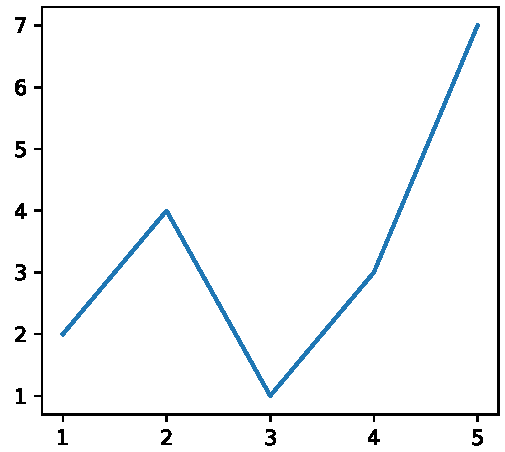
\includegraphics[width=0.7\textwidth]{intro_matplotlib.pdf}
\end{columns}
\end{frame}

\begin{frame}[fragile]
  \frametitle{Enhancing Plots in Matplotlib (2)}
  \begin{columns}
    \column{0.4\textwidth}
  Matplotlib offers various ways to enhance your plots, including adding labels, titles, and grids.\pause
  \begin{lstlisting}[language=Python]
plt.plot(x, y, 'r-o')
plt.xlabel('X-axis label')
plt.ylabel('Y-axis label')
plt.title('Plot Title')
plt.grid(True)
plt.show()
  \end{lstlisting}\pause
   \column{0.5\textwidth}
   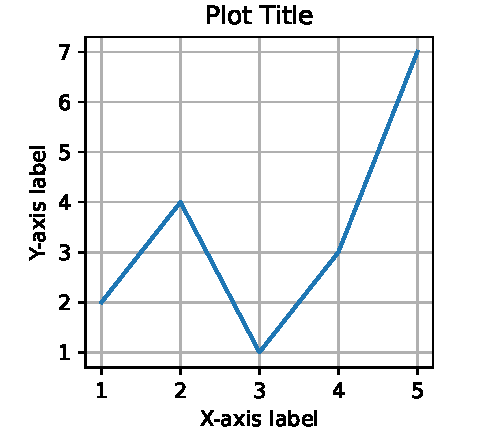
\includegraphics[width=0.6\textwidth]{intro_matplotlib2.pdf}
  \end{columns}

  \begin{columns}
    \column{0.4\textwidth}
  Creating scatter and bar plots:
  \begin{lstlisting}[language=Python]
plt.scatter(x, y, color='red')
plt.show
plt.bar(x, y, color='green')
plt.show()
  \end{lstlisting}
  \column{0.5\textwidth}
  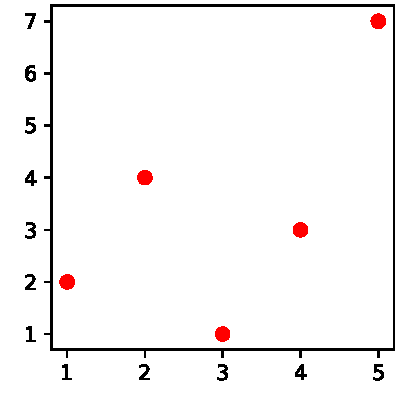
\includegraphics[width=0.4\textwidth]{intro_matplotlib3.pdf}
  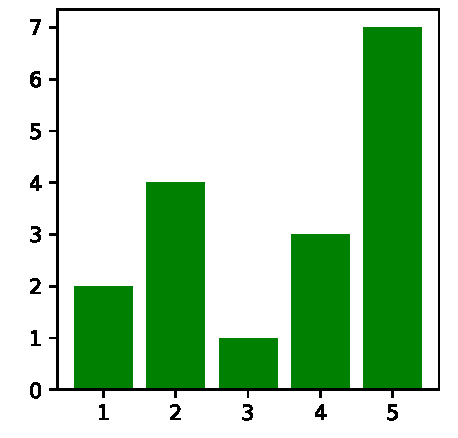
\includegraphics[width=0.4\textwidth]{intro_matplotlib4.pdf}
  \end{columns}
\end{frame}

\begin{frame}
  \frametitle{Some of the plots of Matplotlib}
  \begin{figure}
    \centering
    \begin{minipage}{.25\textwidth}
      \centering
      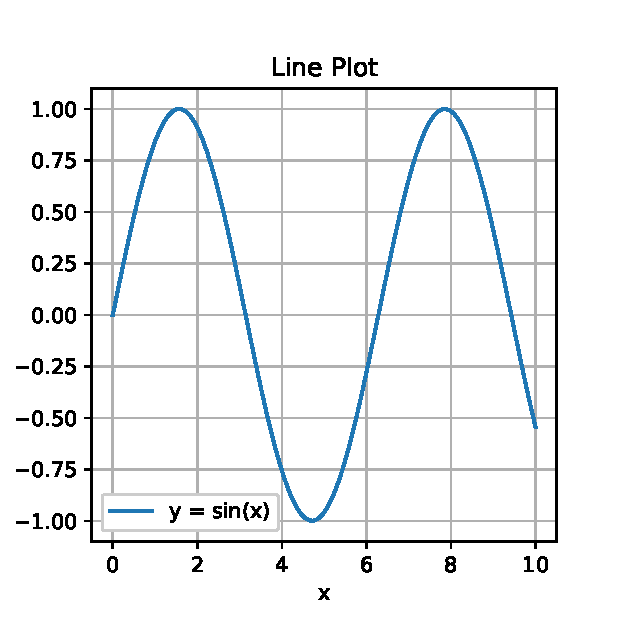
\includegraphics[width=0.99\linewidth]{mpl_plot_examples/line_plot.eps} %FILL IN THE PIC PATH HERE for plot
    \end{minipage}%
    \begin{minipage}{.25\textwidth}
      \centering
      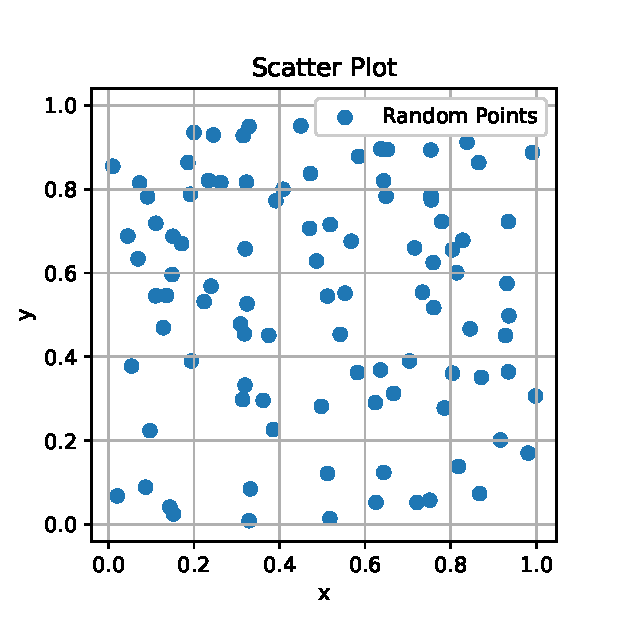
\includegraphics[width=.99\linewidth]{mpl_plot_examples/scatter_plot.eps} %FILL IN THE PIC PATH HERE for scatter
    \end{minipage}
  \end{figure}

  \begin{figure}
    \centering
    \begin{minipage}{.25\textwidth}
      \centering
      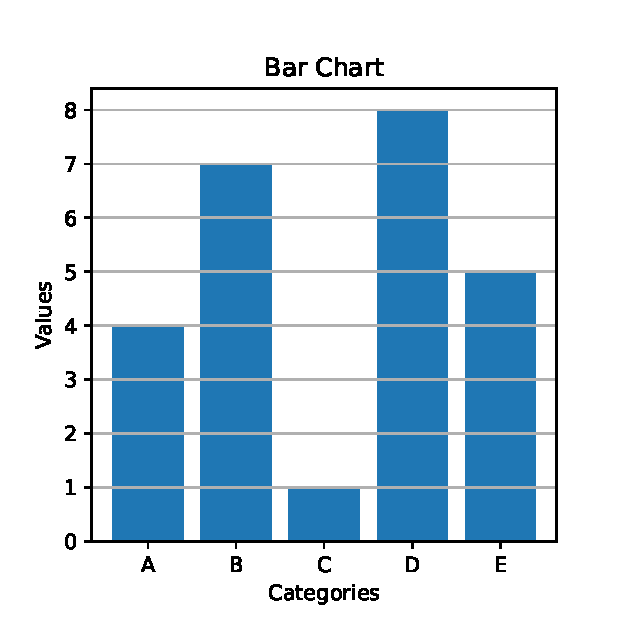
\includegraphics[width=.99\linewidth]{mpl_plot_examples/bar_chart.eps} %FILL IN THE PIC PATH HERE for bar
    \end{minipage}%
    \begin{minipage}{.25\textwidth}
      \centering
      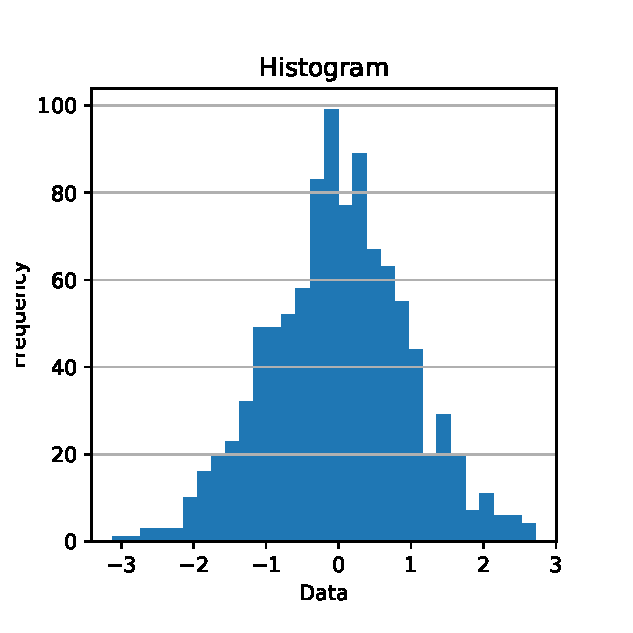
\includegraphics[width=.99\linewidth]{mpl_plot_examples/histogram.eps} %FILL IN THE PIC PATH HERE for hist
    \end{minipage}
    \begin{minipage}{.25\textwidth}
      \centering
      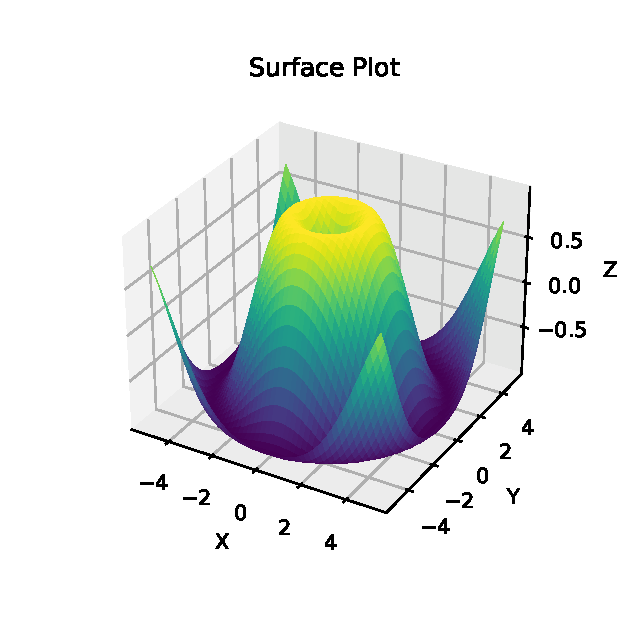
\includegraphics[width=.99\linewidth]{mpl_plot_examples/surface_plot.eps} %FILL IN THE PIC PATH HERE for surface
    \end{minipage}
  \end{figure}
\end{frame}



%%%% ALGORITHMS
% \begin{frame}[fragile]
%  \frametitle{Example algorithm}
%  Compute the factorial of $N$: $N! = N\cdot(N-1)\cdot(N-2)\cdots 2\cdot 1$\\ \vskip1em
%  How to deal with this? \vfill
%  \begin{columns}[T]
%   \column{0.3\textwidth}
%   \begin{block}<2->{Naive approach}
%       \begin{lstlisting}[language=Python,numbers=none]
% Z = 1
% Z = Z*2
% Z = Z*3
% Z = Z*4
% ... etc ...      
%       \end{lstlisting}
%   \end{block}
%   \column{0.3\textwidth}
%   \begin{block}<3->{For-loop}
%       \begin{lstlisting}[language=Python,numbers=none]
% Z = 1;
% for i in range(N):
%     Z = Z*i
%       \end{lstlisting}
%   \end{block}
%   \column{0.3\textwidth}
% \begin{block}<4>{While-loop}
%       \begin{lstlisting}[language=Python,numbers=none]
% Z = 1;
% i = 1;
% while i<=N:
%     Z = Z*i
%     i += 1
%     \end{lstlisting}
%   \end{block}
%  \end{columns}
%  \vspace{0.25cm}
%  \onslide<4>{
%   Note: \lstinline$N$ must be set beforehand!\\ 
%   Note: Pay attention to the relational operators!  }
% \end{frame}

% INPUT AND OUTPUT
\subsection{Input/output}
\begin{frame}[fragile]
  \frametitle{Input and Output in Python (1)}
  Many programs require some input (data) to function correctly. A combination of the following is common:
  \begin{itemize}[<+->]
    \item Input may be given in a parameters file (``hard-coded'')
    \item Input may be entered via the keyboard using the `input` function:
    \begin{lstlisting}[language=Python,numbers=none]
>>> a = input('Please enter a number: ')
    \end{lstlisting}
    \item Input may be read from a file, for instance using Python's built-in open function or libraries like `numpy` for more complex data structures:
    \begin{lstlisting}[language=Python,numbers=none]
>>> with open('myData.txt', 'r') as file:
>>>     data = file.read()
>>> 
>>> import numpy as np
>>> data = np.loadtxt("my_file.csv")
    \end{lstlisting}
    \item There are many other libraries and functions for more advanced input operations, such as json, xml, etc.
  \end{itemize}
 \end{frame}

 \begin{frame}[fragile]
  \frametitle{Input and Output in Python (2)}
  Output of results can be done in several ways, including:
  \begin{itemize}[<+->]
    \item Displaying results to the console - simply omitting a print statement will automatically show expression results in most Python IDEs.
    \item Using the `print` function to show results in the console:
    \begin{lstlisting}[language=Python,numbers=none]
>>> print("The result is:", result)
    \end{lstlisting}
    \item Saving data to a file can be done using various methods including writing to a file or using libraries like pandas for structured data:
    \begin{lstlisting}[language=Python,numbers=none]
>>> with open('output.txt', 'w') as file:
>>> file.write(str(data))

>>> data.save("data.npy")
    \end{lstlisting}
    \item More advanced output methods can utilize libraries such as NumPy, pandas, etc. to save data in various formats including JSON, Excel, etc.
  \end{itemize}
 \end{frame}
 
\subsection{Recursion}
\begin{frame}[label=recursion,fragile]
 \frametitle{Advanced topic: Recursion}
 \begin{columns}
   \column{0.5\textwidth}
   \begin{itemize}
    \item<1-> In order to understand recursion, one must first understand recursion
    \item<2-> A recursive function includes a call to itself (a function within a function)
    \begin{itemize}
      \item<3-> This could lead to infinite calls;
      \item<3-> A base case is required so that recursion is stopped;
      \item<3-> Base case does not call itself, simply returns.
    \end{itemize}
 \end{itemize}
   \column{0.5\textwidth}
   \includegraphics<3>[width=0.7\columnwidth]{scoobydoo.jpg}
 \end{columns}
\end{frame}

\againframe{recursion}

\begin{frame}[fragile]
 \frametitle{Recursion: example}
 \begin{lstlisting}[language=Python]
def mystery(a, b):
  if b == 1:
      # Base case
      return a
  else:
      # Recursive function call
      return a + mystery(a, b-1)
 \end{lstlisting}
\vskip1em \pause
\begin{itemize}
  \item What does this function do? \pause
  \item Can you spot the error? \pause
  \item How deep can you go? Which values of b don't work anymore?
\end{itemize}
\end{frame}

\begin{frame}[fragile]
 \frametitle{Recursion: exercise}
 Create a function computing the factorial of $N$, based on recursion. \pause
 \begin{lstlisting}[language=Python]
def fact_recursive(x):
    # Catch non-integer and negative cases
    if not isinstance(x, int) or x < 0:
        print("You should provide a positive integer number only")
        return None

    # Recursive case
    if x > 1:
        return x * fact_recursive(x - 1)

    # Base case
    else:
        return 1
 \end{lstlisting}
\end{frame}

\section{Conclusions}
\subsection*{Conclusions}
\againframe<2>{contents_prog1}
\begin{frame}[fragile]
  \frametitle{In conclusion...}
  \begin{itemize}
    \colorize<1> \item Python: A versatile development language. Easy to use libraries makes this language multi-purpose and easy to use.
    \colorize<2> \item Programming basics: variables, operators and functions, locality of variables, modules and recursive operations
  \end{itemize}
  \pause
    \begin{itemize}
    \colorize<3> \item For now: exercises on slide deck and Python modules
  \end{itemize}
\end{frame}

\section{Exercises}
\subsection*{Exercise 1}
\begin{frame}[fragile]
  \frametitle{Practice vectors and arrays}
  \begin{enumerate}
    \item Create a list \lstinline|x| with the elements:
    \begin{itemize}
      \item \lstinline|[2, 4, 6, 8, ..., 16]|
      \item \lstinline|[0, 0.5, 2/3, 3/4, ..., 99/100]|
    \end{itemize}
    \item Create a list \lstinline|x| with the elements: \(x_n = \frac{(-1)^n}{2n-1}\) for \(n=1,2,3,\ldots,200\). Find the sum of the first 50 elements \(x_1,\ldots,x_{50}\).
    \item Let \lstinline|x = list(range(20, 201, 10))|. Create a list \lstinline|y| of the same length as \lstinline|x| such that:
    \begin{itemize}
      \item \lstinline|y[i] = x[i] - 3|
      \item \lstinline|y[i] = x[i]| for every even index \(i\) and \lstinline|y[i] = x[i] + 11| for every odd index \(i\).
    \end{itemize}
    \item Let \lstinline|T = np.array([[3, 4, 6], [1, 8, 6], [-4, 3, 6], [5, 6, 6]])|. Perform the following operations on T:
    \begin{itemize}
      \item Retrieve a list consisting of the 2nd and 4th elements of the 3rd row.
      \item Find the minimum of the 3rd column.
      \item Find the maximum of the 2nd row.
      \item Compute the sum of the 2nd column
      \item Compute the mean of the row 1 and the mean of row 4
    \end{itemize}
  \end{enumerate}
 \end{frame}


 \begin{frame}[fragile]
  \frametitle{Practice plotting}
  \begin{enumerate}
    \item Plot the functions $f(x)=x,\ g(x)=x^3,\ h(x)=e^x$ and $z(x)=e^{x^2}$ over the interval $[0,4]$ on the normal scale and on the log-log scale. Use an appropriate sampling to get smooth curves. Describe your plots by using the functions: \lstinline$plt.xlabel$, \lstinline$plt.ylabel$, \lstinline$plt.title$ and \lstinline$plt.legend$.
    \vskip1em
    \item Make a plot of the functions: $f(x)=sin(1/x)$ and $g(x)=cos(1/x)$ over the interval $[0.01,0.1]$. How do you create \lstinline$x$ so that the plots look sufficiently smooth?
  \end{enumerate}
 \end{frame}

 \begin{frame}[fragile]
  \frametitle{Practice control flow and loops (1)}
  \begin{enumerate}
    \item Write a function that uses two logical input arguments with the following behaviour:
    \begin{align*}
       f(\text{true},\text{true}) \mapsto \text{false} \\
      f(\text{false},\text{true}) \mapsto \text{true} \\ 
      f(\text{true},\text{false}) \mapsto \text{true} \\
      f(\text{false},\text{false}) \mapsto \text{false} \\
    \end{align*}
    \item Write a function that computes the factorial of x:
    \[ f(x) = x! = 1 \times 2 \times 3 \times 4 \times \ldots \times x \]
    \begin{itemize}
      \item Using a loop-construction
      \item Using recursion
    \end{itemize}
  \end{enumerate}
 \end{frame}

 \begin{frame}[fragile]
  \frametitle{Practice control flow and loops (2)}
  \begin{enumerate}
    \item Write a function that computes the exponential function using the Taylor series
    \[  e^x = 1 + x + \frac{x^2}{2!} + \frac{x^3}{3!} + \ldots \]
    until the last term is smaller than $10^{-6}$.
    \item Use a script to compute the result of the following series:
    \[
      f_n = \sum_{n=1}^{\infty} \frac{1}{\pi^2 n^2}
    \]
    This should give you an indication of the fraction this series converges to.
    \begin{itemize}
      \item Now plot in two vertically aligned subplots i) The result as a function of $n$, and ii) the difference with the earlier mentioned fraction as a function of n. For the latter, consider carefully the axis scale!
      % \item Use \lstinline$tic$ and \lstinline$toc$ to compare the computing times with $\pi^2$ inside vs outside the loop.
    \end{itemize}
  \end{enumerate}
 \end{frame}

 \begin{frame}[fragile]
  \frametitle{Practice logical indexing}
  \begin{enumerate}
    \item Let \lstinline$x = np.linspace(-4,4,1000)$, $y_1 = 3x^2 - 4x - 6$ and $y_2 = 1.5x - 1$. Use logical indexing to determine function $y_3 = \mathrm{max}(\mathrm{max}(y_1,y_2),0)$. Plot the function.
    \item Consider these data concerning the age (in years), length (in cm) and weight (in kg) of twelve adult men: \lstinline$A = [41 25 33 29 64 34 47 38 49 32 26 26]; H = [165 186 177 190 156 174 164 205 184 190 165 171]; W = [75 90 97 60 74 65 101 85 91 75 87 70];$.
    \begin{itemize}
      \item Calculate the average of all vectors (age, weight and length).
      \item Combine the command \lstinline$length$ with logical indexing to determine how many men in the group are taller than 182 cm.
      \item What is the average age of men with a body-mass index ($B \equiv \frac{W}{L^2}$ with $W$ in kg and $L$ in m) larger than 25? And for men with a $B<25$?
      \item How many men are older than the average and at the same time have a BMI below 25?
    \end{itemize}
  \end{enumerate}
 \end{frame}

\begin{frame}[fragile]
  \frametitle{Practice algorithm: Fourier series for heat equation}
  The unsteady 1D heat equation in 1D in a slab of material is given as:
  \[
     \frac{\partial T}{\partial t} = k\frac{\partial^2 T}{\partial x^2}
  \]
 We can express the temperature profile $T(x,t)$ in the slab using a Fourier sine series. For an initial profile T(x,0) = 20 and fixed boundary values T(0,t) = T(L,t) = 0, the solution is given as:
  \[
     T(x,t) = \sum_{n=1}^{n=\infty}\frac{40(1-(-1)^n)}{n\pi}  \sin\left(\frac{n\pi x}{L}\right) \exp\left(-kt\frac{n \pi}{L}^2\right)
  \]
  \begin{itemize}
      \item Create a script to solve this equation using loops and/or conditional statements
  \end{itemize}
 \end{frame}
 
%  \begin{frame}[fragile]
%   \frametitle{Fourier series for heat equation (1)}
%   A simple construct with a double loop.
%    \begin{lstlisting}
%  L = 2;
%  k = 0.004;
%  t = 3;
%  x = 0:0.1:L;
%  s = 0;
 
%  for n = 1:50
%      for i = 1:length(x)
%          pt(i) = 40*(1-(-1)^n)/(n*pi) * sin(n*pi*x(i)/L) * exp(-k*t*(n*pi/L)^2);
%      end
%      s = s + pt;
%  end
 
%  plot(x,s)
%    \end{lstlisting}
%  \end{frame}
 
%  \begin{frame}[fragile]
%   \frametitle{Fourier series for heat equation (2-1)}
%  We can also solve the equation for the entire x-range in 1 go. \lstinline$part$ and $s$ are both vectors. This is more efficient.
%    \begin{lstlisting}
%  L =  2;
%  x = linspace(0,L,101);
%  k = 0.004;
%  t = 3;
 
%  s = 0;
%  for n = 1:50
%      part = 40*(1-(-1)^n)/(n*pi) * sin(n*pi*x/L) * exp(-k*t*(n*pi/L)^2);
%      s = s + part;
%  end
 
%  plot(x,s)
%    \end{lstlisting}
%  \end{frame}
 
%  \begin{frame}[fragile]
%   \frametitle{Fourier series for heat equation (2-2)}
%  We can break the for-loop when the calculations are precise enough using an if-statement and a break-command.
%    \begin{lstlisting}
%  L = 2;
%  x = linspace(0,L,101);
%  k = 0.004;
%  t = 3;
 
%  s = 0;
%  for n = 1:2:50
%      part = 40*(1-(-1)^n)/(n*pi) * sin(n*pi*x/L) * exp(-k*t*(n*pi/L)^2);
%      s = s + part;
%      if (max(abs(part)) < 1e-6)
%          n
%          break
%      end
%  end
 
%  plot(x,s)
%    \end{lstlisting}
%  \end{frame}
 
%  \begin{frame}[fragile]
%   \frametitle{Fourier series for heat equation (3-1)}
%  We can run a while-loop for indeterminate iterations to ensure a certain precision while keeping computational demands to a minimum:
%    \begin{lstlisting}
%  L =  2;
%  x = linspace(0,2,101);
%  k = 0.004;
%  t = 3;
 
%  s = 0;
%  n = 1;
%  part = 1;
%  while (max(abs(part))>1e-6)
%      part = 40*(1-(-1)^n)/(n*pi) * sin(n*pi*x/L) * exp(-k*t*(n*pi/L)^2)
%      s = s + part;
%      n = n + 2;
%  end
 
%  n
%  plot(x,s)
%    \end{lstlisting}
%  \end{frame}
 
%  \begin{frame}[fragile]
%   \frametitle{Fourier series for heat equation (3-2)}
%  The \lstinline$drawnow$ command makes sure a plot is drawn before subsequent commands are executed. This gives us insight in the iteration process:
%    \begin{lstlisting}
%  L =  2;
%  x = linspace(0,2,101);
%  k = 0.004;
%  t = 3;
 
%  s = 0;
%  n = 1;
%  part = 1;
%  while (max(abs(part))>1e-6)
%      part = 40*(1-(-1)^n)/(n*pi) * sin(n*pi*x/L) * exp(-k*t*(n*pi/L)^2)
%      s = s + part;
%      n = n + 2;
%      plot(x,s)
%      pause(0.4)
%      drawnow
%  end
 
%  n
%    \end{lstlisting}
%  \end{frame}

%  \begin{frame}[fragile]
%   \frametitle{Fourier series for heat equation (as a function)}
%  A rudimentary function (i.e. no comments or checks) to get the heat equation profile for a given length, heat diffusivity and time:
%    \begin{lstlisting}
%  function [s,x] = fourier_series_heat_eqn(L,k,t)
%  x = linspace(0,L,101);
 
%  s = 0;
%  n = 1;
%  part = 1;
%  while (max(abs(part))>1e-6)
%      part = 40*(1-(-1)^n)/(n*pi) * sin(n*pi*x/L) * exp(-k*t*(n*pi/L)^2);
%      s = s + part;
%      n = n + 2;
%  end
%    \end{lstlisting}
   
%  Calling the function from a different script multiple times to plot a transient profile:
%  \begin{lstlisting}
%  for t = 0.01:0.01:30
%      [solution,xvec] = fourier_series_heat_eqn(2,0.004,t);
%      plot(xvec,solution)
%      xlabel('Position [m]');
%      ylabel('Temperature [^\circC]');
%      drawnow
%  end
%  \end{lstlisting}
%  \end{frame}

% \end{document}


% References
% http://ocw.mit.edu/courses/electrical-engineering-and-computer-science/6-00sc-introduction-to-computer-science-and-programming-spring-2011/unit-1/lecture-1-introduction-to-6.00/
% http://www.greenteapress.com/thinkpython/html/thinkpython002.html
% https://www.youtube.com/channel/UCLMQ21H2ad95faYG3yGCwYA
%http://stackoverflow.com/questions/4227145/in-Python-are-variables-really-double-precision-by-default
%http://www.exploringbinary.com/why-0-point-1-does-not-exist-in-floating-point/



\title{Matlab and Programming 2}
\subtitle{Advanced programming techniques}
\lecture{Programming 2}{programming2}
\part{Python programming II}
\section{Coding style}
\subsection*{Introduction}
\begin{frame}[label=contents_prog2]
  \frametitle{Today's outline}
  \mode<beamer>{
    \only<1>{\tableofcontents}
  }
  \only<2>{\tableofcontents[currentsection]}
\end{frame}

\subsection*{Program design}
\begin{frame}[label=workrightfast]
  \frametitle{Make a habit of the following adage}
  \begin{center}
    
\includegraphics[width=0.8\textwidth]{workrightfast.pdf}
  \end{center}
\end{frame}

{\nologo
\begin{frame}[label=work-explain]
  \frametitle{Make it work}
  Use the building blocks of previous lecture to create an algorithm:
  \begin{enumerate}
    \colorize<1> \item \emph{Problem analysis}\\ Contextual understanding of the nature of the problem to be solved
    \colorize<2> \item \emph{Problem statement}\\ Develop a detailed statement of the mathematical problem to be solved with the program
    \colorize<3> \item \emph{Processing scheme}\\ Define the inputs and outputs of the program
    \colorize<4> \item \emph{Algorithm}\\ A step-by-step procedure of all actions to be taken by the program (\emph{pseudo-code})
    \colorize<5> \item \emph{Program the algorithm}\\ Convert the algorithm into a computer language, and debug until it runs
    \colorize<6> \item \emph{Evaluation}\\ Test all of the options and conduct a validation study
  \end{enumerate}
  \vskip1em
  Now it's time to make it right!
\end{frame}
}
% \subsection*{Program design and coding style}
% \begin{frame}
%   \frametitle{It's a bit disturbing but...}
%   \begin{center}
%     {\LARGE Your code will not be understood by anyone\\}
%   \pause
%   \vskip1em
%   That includes future-you
%   \vskip2em
%   \end{center}
% \end{frame}

\subsection*{Example code}
\begin{frame}[fragile]
 \frametitle{Interpret the following code}
 \begin{lstlisting}[language=Python]
s = checksc()
if s:
    a = cb()
    b = cfrsp()
    if a < 5:
        if b > 5:
            a = gtbs()
        if a > b:
            ubx()
else:
    brn()
    gtbs()
 \end{lstlisting}
\end{frame}

\begin{frame}[plain]
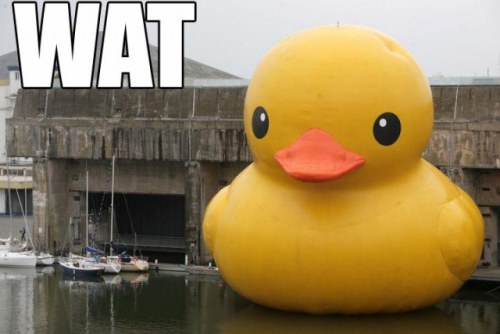
\includegraphics[keepaspectratio=true,width=\textwidth]{wat-2.jpg}
\end{frame}

\begin{frame}[fragile]
 \frametitle{Enhancing Readability with Proper Indentation}
 Proper indentation is not just about syntax in Python; it significantly impacts the readability of the code. Python recommends 4 spaces for indentation. Let's see the difference:
 \pause
 \begin{columns}[T]
    \column{0.5\textwidth}
     \begin{lstlisting}[language=Python,basicstyle=\small]
s = checksc()
if s:
a = cb()
b = cfrsp()
if a < 5:
if b > 5:
a = gtbs()
if a > b:
ubx()
else:
brn()
gtbs()
 \end{lstlisting}
    \column{0.5\textwidth}
     \begin{lstlisting}[language=Python,basicstyle=\small]
s = checksc()
if s:
    a = cb()
    b = cfrsp()
    if a < 5:
        if b > 5:
            a = gtbs()
        if a > b:
            ubx()
else:
    brn()
    gtbs()
 \end{lstlisting}
 \end{columns}
\end{frame}

\begin{frame}[fragile]
 \frametitle{Readable Variables and Function Names}
 Making use of descriptive variable and function names enhances the readability and understanding of the code. 
 \begin{columns}[T]
    \column{0.5\textwidth}
\begin{lstlisting}[language=Python, basicstyle=\scriptsize]
s = checksc()
if s:
    a = cb()
    b = cfrsp()
    if a < 5:
        if b > 5:
            a = gtbs()
        if a > b:
            ubx()
else:
    brn()
    gtbs()
 \end{lstlisting}
    \column{0.5\textwidth}
     \begin{lstlisting}[language=Python, basicstyle=\scriptsize]
isAvailable = checkSchedule()
if isAvailable:
    bookCount = countBooks()
    freeShelfSpace = checkFreeShelfSpace()
    if bookCount < 5:
        if freeShelfSpace > 5:
            bookCount = visitBookStore()
        if bookCount > freeShelfSpace:
            useStorageBox()
else:
    burnBooks()
    visitBookStore()
 \end{lstlisting}
 \end{columns}
\end{frame}

\begin{frame}[fragile]
 \frametitle{Avoiding Magic Numbers in the Code}
 Magic numbers are constant values without a name, which can reduce code readability. Replacing them with named constants can enhance the understanding of the code.
 \begin{columns}[T]
    \column{0.5\textwidth}
     \begin{lstlisting}[language=Python,basicstyle=\scriptsize]
isAvailable = checkSchedule()
if isAvailable:
    bookCount = countBooks()
    freeShelfSpace = checkFreeShelfSpace()
    if bookCount < 5:
        if freeShelfSpace > 5:
            bookCount = visitBookStore()
        if bookCount > freeShelfSpace:
            useStorageBox()
else:
    burnBooks()
    visitBookStore()
 \end{lstlisting}
    \column{0.5\textwidth}
     \begin{lstlisting}[language=Python,basicstyle=\scriptsize,emph={MIN_BOOKS_REQUIRED,MAX_SHELF_SPACE},emphstyle=\color{red}]
MAX_SHELF_SPACE = 5
MIN_BOOKS_REQUIRED = 5

isAvailable = checkSchedule()
if isAvailable:
    bookCount = countBooks()
    freeShelfSpace = checkFreeShelfSpace()
    if bookCount < MAX_SHELF_SPACE:
        if freeShelfSpace > MIN_BOOKS_REQUIRED:
            bookCount = visitBookStore()
        if bookCount > freeShelfSpace:
            useStorageBox()
else:
    burnBooks()
    visitBookStore()
 \end{lstlisting}
 \end{columns}
\end{frame}

\begin{frame}[fragile]
 \frametitle{Now, That's More Like It!}
 Demonstrating the evolution of the script to a more readable and maintainable version.
 \begin{columns}[T]
    \column{0.3\textwidth}
     \begin{lstlisting}[language=Python]
s = checksc()
if s:
    a = cb()
    b = cfrsp()
    if a < 5:
        if b > 5:
            a = gtbs()
        if a > b:
            ubx()
else:
    brn()
    gtbs()
 \end{lstlisting}
    \column{0.7\textwidth}
     \begin{lstlisting}[language=Python]
MAX_SHELF_SPACE = 5
MIN_BOOKS_REQUIRED = 5

isAvailable = checkSchedule()
if isAvailable:
    bookCount = countBooks()
    freeShelfSpace = checkFreeShelfSpace()
    if bookCount < MAX_SHELF_SPACE:
        if freeShelfSpace > MIN_BOOKS_REQUIRED:
            bookCount = visitBookStore()
        if bookCount > freeShelfSpace:
            useStorageBox()
else:
    burnBooks()
    visitBookStore()
 \end{lstlisting}
 \end{columns}
\end{frame}


%% ASPECTS OF A GOOD PROGRAM
\subsection*{Aspects of a good program}
\begin{frame}
  \frametitle{Writing readable code}
  Good code reads like a book.\vskip2em \pause
  \begin{itemize}
    \item When it doesn't, make sure to use comments. In Python, everything following \lstinline$ \# is a comment$
    \item Prevent ``smart constructions'' in the code
    \item Re-use working code (i.e. create functions for well-defined tasks).
    \item Documentation is also useful, but hard to maintain.
    \item Python comes with a function that generates reports from comments
  \end{itemize}
\end{frame}

\begin{frame}[fragile]
  \frametitle{How not to comment}
  \begin{itemize}[<+->]
   \item Useless:
   \begin{lstlisting}
# Start program 
   \end{lstlisting}
   \item Obvious:
   \begin{lstlisting}
if (a > 5)   # Check if a is greater than 5
    ... 
 \end{lstlisting}
   \item Too much about the life:
   \begin{lstlisting}[basicstyle=\tiny\ttfamily]
# Well... I do not know how to explain what is going on
# in the snippet below. I tried to code in the night 
# with some booze and it worked then, but now I have a 
# strong hangover and some parameters still need to be
# worked out...
   \end{lstlisting}
 
   \item ...
   \begin{lstlisting}[basicstyle=\tiny\ttfamily]
# You may think that this function is obsolete, and doesn't seem to
# do anything. And you would be correct. But when we remove this 
# function for some reason the whole program crashes and we can't 
# figure out why, so here it will stay.
   \end{lstlisting}
  \end{itemize}
 \end{frame}
 
 \begin{frame}[fragile]
  \frametitle{Adding comments to our Python program}
  \centering\tikz{\node[emphblock, text width=0.7\textwidth]{Use comments to document design and purpose (functionality), not mechanics (implementation).};}
  \begin{lstlisting}
IAmFree = checkSchedule()
if IAmFree:
    # Count books and amount of free space on a shelf. 
    # If minimum number of books I need is less than a 
    # shelf capacity, go shopping and buy additional 
    # literature. If the amount of books after the 
    # shopping is too big, use boxes to store them.
    books = countBooks()
    shelfSize = countFreeSpaceShelf()
    
    ...
    
else:
    burnBooks()
    goToBookStore()
 \end{lstlisting}
 \end{frame}
 

% \begin{frame}
%   \frametitle{If anything sticks today, let it be this}
%   \begin{center}
%     {\LARGE Your code will not be understood by anyone\\}
%   \pause
%   \vskip1em
%   That includes future-you
%   \vskip2em
%   \end{center}
%   \pause
%   \tikz{\node[emphblock, text width=\textwidth]{Use comments and code to document design and purpose (functionality), not mechanics (implementation).};}
%   \vskip1em\pause
%   \tikz{\node[emphblock, text width=\textwidth]{Use consistent and sensible naming of functions and variables.};}
% \end{frame}

\begin{frame}
  \frametitle{What else makes a good program?}
  \begin{columns}[T]
        \column{0.5\textwidth}
        \begin{itemize}
            \item Portability (guaranteed in Python)
            \item Readability
            \item Efficiency 
            \item Structural
            \item Flexibility
            \item Generality
            \item Documentation
        \end{itemize}
        \column{0.5\textwidth}
Funny thing is: This list does not mention that the program should be actually working for its intended purposes!
    \end{columns}
\end{frame}


\begin{frame}[fragile]
  \frametitle{Readability}
  Don't use meaningless variable or function names. Rule of thumb: use verbs for functions and nouns for variables.
  \vspace*{2em}
  \begin{lstlisting}[language=Python]
# stupid names
x = 5;
xx = myfunction(x);

# proper names
number_dams = 6;
beaver_workforce = allocate_beavers();
dams = build_dams(beaver_workforce, number_dams);
  \end{lstlisting}
\end{frame}

\begin{frame}[fragile]
  \frametitle{Efficiency}
  This one is difficult. Not much you can do without truly understanding how Python is utilizing your processor and memory. A couple of guidelines though:
  \begin{itemize}
      \item Avoid loops
      \item Especially avoid nested loops
      \item Use inherent matrix operations when possible
      \item Reduce IO (i.e. reading / writing to and from files)
      \item Don't run scripts from network disks
      \item Pre-allocate your arrays, that means, making it as large as the maximum required size for your particular problem
      \item Use Python's built-in modules for performance profiling, such as cProfile or timeit, to test the execution times
  \end{itemize}
\end{frame}

\begin{frame}[fragile]
  \frametitle{Efficiency: Measuring execution time example}
  \begin{columns}
    \column{0.5\textwidth}
    \begin{lstlisting}[language=Python]
import numpy as np
import time

x = np.linspace(0, 10, 1000001)
start_time = time.time()

y = []
for cr in range(len(x)):
    y.append(np.sin(2 * np.pi * x[cr]))

end_time = time.time()
print(f'Execution time: {end_time - start_time} seconds')
    \end{lstlisting}
    \column{0.5\textwidth}
    \begin{lstlisting}[language=Python]
import numpy as np
import time

x = np.linspace(0, 10, 1000001)
start_time = time.time()

y = np.sin(2 * np.pi * x)

end_time = time.time()
print(f'Execution time: {end_time - start_time} seconds')
    \end{lstlisting}
  \end{columns}
\end{frame}


\begin{frame}[fragile]
  \frametitle{Structural}
  \begin{itemize}
      \item Compartmentalize your code.
      \item Write functions whenever possible.
      \begin{itemize}
        \item If you have $>15$ lines of code, you can probably replace it by one or more functions.
        \item In principle, it should not even matter how function works, as long as it gives the expected output.\\ \vskip1ex
        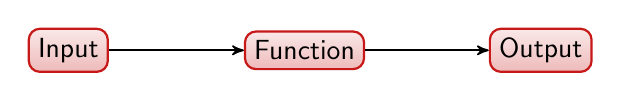
\begin{tikzpicture}[node distance = 3cm, auto]
          % Place nodes
          \node [emphblock] (function) {Function};
          \node [emphblock, left of=function] (input) {Input};
          \node [emphblock, right of=function] (output) {Output};
          % Draw edges
          \draw [line,->] (input) -> (function);
          \draw [line,->] (function) -> (output);
      \end{tikzpicture}\vskip1ex
      \end{itemize}
      \item Put critical variables at the beginning of your program.
  \end{itemize}  
\end{frame}

\begin{frame}[fragile]
  \frametitle{Structural}
    Write code as though it were paragraphs in a story.
    \begin{lstlisting}[language=Python,basicstyle=\scriptsize]
from dependencies import * # importing all dependencies

# Step 0: Define variables
n_steps = 10000  # number of steps
n_walks = 1000  # number of random walk samples

# Step 1: Generate n_walks number of random walks
de = np.zeros((n_walks, 2))
for i in range(n_walks):
    angles = get_random_angles(n_steps)
    coord = transform_angles_to_coordinates(angles)
    de[i, 0] = calculate_de(coord)  # store de
    de[i, 1] = de[i, 0]**2  # store de^2

# Step 2: Plot the histogram
plt.hist(de[:, 0], density=True)
D, P = calculate_pdf(n_steps, 1000)
plt.plot(D, P)
plt.show()
    \end{lstlisting}
\end{frame}


\begin{frame}[fragile]
  \frametitle{Flexibility}
    If you want to add a feature or change something inside the program, it should not require rewriting the whole program. (jargon: non-linear propagation of change).\\
    
    Solution: Encapsulate your code and "Don't Repeat Yourself"
    \begin{itemize}
        \item Use functions for specific tasks (can you verbalize it? Then it is probably a function)
        \item Use variables, even for constants (it sounds like a oxymoron, but it's not! In fact, constant variables are a real thing)
        \item Use abstraction whenever possible
    \end{itemize}
\end{frame}

\begin{frame}[fragile]
  \frametitle{Generalization}
    If your code works for one problem, it should also work for a similar problem, whether it's in another company or on another planet. \\ \vskip1em
    
    Pro-tip: Separate data from algorithms.\\
    
    To be honest, I rarely see students making this mistake.
    
\begin{lstlisting}
# Stupid code
A = [[1, 2, 3], [4, 5, 6], [7, 8, 9]]  # Hardcode data in the program
    
# Smart code
with open('some_random_dataset.dat') as file:
    data = file.read()  # or use appropriate data loading functions from libraries like pandas
\end{lstlisting}
\end{frame}


\begin{frame}[fragile]
  \frametitle{Documentation}
    Properly document your code. Write your comments in a clear and concise fashion. Help your future self: Write clear and concise documentation.
    \begin{columns}
    \column{0.6\textwidth}
    \begin{lstlisting}[language=Python]
def f(a, b=None):
    if b is not None:
        c = a + b
    elif b is None and a is not None:
        c = a + a
    else:
        c = 0
    return c
    \end{lstlisting}
    \column{0.4\textwidth}
    
\includegraphics[width=\columnwidth]{figures/drakeno.jpg}
    \end{columns}
\end{frame}

\begin{frame}[fragile]
  \frametitle{Documentation}
    Properly document your code. Write your comments in a clear and concise fashion. Help your future self: Write clear and concise documentation.
    \begin{columns}
    \column{0.6\textwidth}
    \begin{lstlisting}[language=Python,basicstyle=\scriptsize]
def f(a, b=None):
    """
    Add two values together.
    
    Parameters:
    a: The first number.
    b: The second number. Optional.
    
    Returns:
    The sum of a and b, or 2*a if b is not given, or 0 if a is not given.
    
    See also: sum, operator.add
    """
    if b is not None:
        c = a + b  # sum two different numbers
    elif b is None and a is not None:
        c = a + a  # double single number
    else:
        c = 0      # input not valid
    return c
    \end{lstlisting}
    \column{0.4\textwidth}
    
\includegraphics[width=\columnwidth]{figures/drakeyes.jpg}
    \end{columns}
\end{frame}


\againframe{workrightfast}

\begin{frame}[fragile,label=wrf-explain]
  \frametitle{Make a habit of the following adage}
  \begin{enumerate}
    \colorize<1> \item \emph{Make it work}\\ 
    Create an algorithm that does the intended job. Make sure it works, and works repeatedly. Test and verify frequently. Add \emph{todo} comments when you're not sure about a certain decision.
    \colorize<2> \item \emph{Make it right}\\ 
    Refactor the code to improve the code design. Insert functions, comments, compartmentalize it. Get rid of magic numbers, use sensible variable names. Check input. Test and verify. Align with the team!
    \colorize<3> \item \emph{Make it fast}\\ 
    Measure and tune the performance of your code (profiling tool). In Python, vectorized calculations are much (!) faster than for-loops. Use sensible numerical techniques (e.g. higher-order integration).
  \end{enumerate}
  Program by iterating over these aspects multiple times, starting at the fine-grained level, working your way up.
\end{frame}

% \begin{frame}
% \frametitle{Code organization}
%   \begin{itemize}
%     \item Optimization of a code is time-consuming and complicated
%     \item The more you optimize your code, the less readable it becomes
%     \item But... You can write it in a such way that it will be flexible and easy to maintain
%     \item Especially important in team work
%     \item Any person has its own handwriting. Any programmer has its own coding style.
% \end{itemize}
%  \tikz{\node[emphblock,text width=\textwidth]{The coding style $\equiv$ handwriting...};}
% \end{frame}

\section{Debugging and profiling}
\subsection*{Errors in programming}
\againframe<2>{contents_prog2}
\begin{frame}
 \frametitle{Errors in computer programs}
 \footnotesize\selectfont
 The following symptoms can be distinguished:
 \begin{itemize}
   \item Unable to execute the program
   \item Program crashes, warnings or error messages
   \item Never-ending loops
   \item Wrong (unexpected) result
 \end{itemize}
 \vskip1em
 \uncover<2->{
  Three error categories:
  \begin{description}
   \colorize<2->  \item[Syntax errors] You did not obey the language rules. These errors prevent running or compilation of the program.
   \colorize<3->  \item[Runtime errors] Something goes wrong during the execution of the program resulting in an error message (problem with input, division by zero, loading of non-existent files, memory problems, etc.)
   \colorize<4->  \item[Semantic errors] The program does not do what you expect, but does what have told it to do.
  \end{description}
 }
\end{frame}

% \begin{frame}[fragile]
%  \frametitle{Verification and validation}
%   \scriptsize\selectfont
%   \begin{columns}
%     \column{0.6\textwidth}
%     \uncover<3->{\begin{block}{Verification}
%     Verification is the process of mathematically and computationally assuring that the model computes what you have entered.    
%     \end{block}
%     }
%     \uncover<7->{
%     \begin{block}{Validation}
%       Validation is the process of determining the degree to which a model is an accurate representation of the real world from the perspective of the intended uses of the model
%     \end{block}
%     }
% 
%   \column{0.4\textwidth}
%     \begin{tikzpicture}[block/.style={rectangle,minimum size=3mm,text badly centered,drop shadow,
% 					thick,rounded corners,draw=maincolor,top color=maincolor!35,bottom color=maincolor!20,
% 					font=\sffamily\scriptsize},>=stealth,node distance=0.75cm]
% 	\node[block] (p) at (0,0) {Problem};
% 	\uncover<2->{\node[below of=p] (p1) {};
% 	\node[block, below of=p1] (mm) {Mathematical Model};
% 	\node[below of=mm] (mm1) {};}
% 	\uncover<4->{\node[block, below of=mm1] (cm) {Computational Model};
% 	\node[below of=cm] (cm1) {};}
% 	\uncover<6->{\node[block, below of=cm1] (r) {Results};}
% 	
% 	\uncover<3->{\node[block, left of=p1,node distance=2cm] (v1) {Verification};}
% 	\uncover<5->{\node[block, left of=mm1,node distance=2cm] (v2) {Verification};}
% 	\uncover<7->{\node[block, left of=cm1,node distance=2cm] (v3) {Validation};}
% 	
% 	\uncover<2->{\draw[->] (p) -> (mm);}
% 	\uncover<4->{\draw[->] (mm) -> (cm);}
% 	\uncover<6->{\draw[->] (cm) -> (r);}
% 	
% 	\uncover<3->{\draw[->] (v1) -> (p1);}
% 	\uncover<5->{\draw[->] (v2) -> (mm1);}
% 	\uncover<7->{\draw[->] (v3) -> (cm1);}
%     \end{tikzpicture}
%   \end{columns}
% 
% \end{frame}
% % 
% 
% \begin{frame}
%   \frametitle{Be aware of your uncertainties}
%   \scriptsize\selectfont
%   \begin{columns}
%     \column{0.5\textwidth}
%     \begin{center}
%       \mode<beamer>{
% 	\includegraphics<1>[width=0.8\columnwidth]{ptolemy1-1}
% 	\includegraphics<2>[width=0.8\columnwidth]{ptolemy1-2}
% 	\includegraphics<3>[width=0.8\columnwidth]{ptolemy1-3}
% 	\includegraphics<4>[width=0.8\columnwidth]{ptolemy1-4}
% 	\includegraphics<5>[width=0.8\columnwidth]{ptolemy1-5}
% 	\includegraphics<6>[width=0.8\columnwidth]{ptolemy1-6}
%       }
%       \includegraphics<7->[width=0.8\columnwidth]{ptolemy1-7}
%     \end{center}
%     \column{0.5\textwidth}
%     \begin{center}
%       \mode<beamer>{
% 	\includegraphics<7>[width=0.8\columnwidth]{ptolemy2-0}
% 	\includegraphics<8>[width=0.8\columnwidth]{ptolemy2-1}
% 	\includegraphics<9>[width=0.8\columnwidth]{ptolemy2-2}
% 	\includegraphics<10>[width=0.8\columnwidth]{ptolemy2-3}
% 	\includegraphics<11>[width=0.8\columnwidth]{ptolemy2-4}
% 	\includegraphics<12>[width=0.8\columnwidth]{ptolemy2-5}
% 	\includegraphics<13>[width=0.8\columnwidth]{ptolemy2-6}
%       }
%       \includegraphics<14>[width=0.8\columnwidth]{ptolemy2-7}
%     \end{center}
%   \end{columns}
%   \begin{itemize}
%     \item<7-> The perceived orbit of Mars from Earth shows a zig-zag (in contrast to the Sun, Mercury, Venus)
%     \item<14> Even though they were not 'right', Earth-centered models (Ptolemy) were still valid
%   \end{itemize}
% \end{frame}
% 
% \begin{frame}
%   \frametitle{Be aware of your uncertainties}
%   \vfill
%   \begin{block}{Aleatory uncertainty}
%     Uncertainty that arises due to inherent randomness of the system, features that are too complex to measure and take into account
%   \end{block}
%   \vskip1em
%   \begin{block}{Epistemic uncertainty}
%       Uncertainty that arises due to lack of knowledge of the system, but could in principle be known
%   \end{block}
%   \vfill
% \end{frame}

%  
\subsection*{Debugging and profiling}
\begin{frame}
  \frametitle{Validation}
  \begin{itemize}
    \item Testcases: run the program with parameters such that a known result is (should be) produced.
    \item Testcases: what happens when unforeseen input is encountered?
    \begin{itemize}
      \item More or fewer arguments than anticipated? (Python uses \lstinline$*args$ and \lstinline$**kwargs$ to create a varying number of input arguments, and to check the number of given input arguments
      \item Other data types than anticipated? How does the program handle this? Warnings, error messages (crash), NaN or worse: a program that silently continues?
    \end{itemize}
    \item For physical modeling, we typically look for analytical solutions
    \begin{itemize}
      \item Sometimes somewhat stylized cases
      \item Possible solutions include Fourier-series
      \item Experimental data
    \end{itemize}
    \vskip1ex
  \end{itemize}
  \pause
  \tikz{\node[emphblock] {\large But: validation can only tell you \emph{if} something is wrong, not \emph{where} it went wrong.}}
\end{frame}

\begin{frame}
\frametitle{The debugger (1)}
\begin{itemize}
  \colorize<1-> \item No-one can write a 1000-line code without making errors
  \begin{itemize}
    \colorize<1-> \item If you can, please come work for us
  \end{itemize}
  \colorize<2-> \item One of the most important skills you will acquire is debugging.
  \colorize<3-> \item Although it can be frustrating, debugging is one of the most intellectually rich, challenging, and interesting parts of programming.
  \colorize<4-> \item In some ways, debugging is like detective work. You are confronted with clues, and you have to infer the processes and events that led to the results you see.
  \colorize<5-> \item Actually, you are the detective, the murderer and the victim at the same time.
\end{itemize}
\onslide<5>{
\vskip1em
\begin{raggedleft}
\emph{``When you have eliminated the impossible, whatever remains, however improbable, must be the truth.''}
\\
--- A. Conan Doyle, The Sign of Four\\ % http://www.greenteapress.com/thinkpython/html/thinkpython002.html
\end{raggedleft}
}
\end{frame}

\begin{frame}
  \frametitle{The debugger (2)}
A debugger can help you to:
\begin{itemize}
  \item Pause a program at a certain line: set a \emph{breakpoint}
  \item Check the values of variables during the program
  \item Controlled execution of the program:
  \begin{itemize}
    \item One line at a time
    \item Run until a certain line
    \item Run until a certain condition is met (conditional breakpoint)
    \item Run until the current function exits
  \end{itemize}
  \item Note: You may end up in the source code of Python functions!
  \item Check Canvas (Python Crash Course section) for a demonstration of the debugger.
\end{itemize}
\end{frame}

{\nologo
\begin{frame}[fragile]
  \frametitle{Recursive Fibonacci}
  \begin{itemize}
    \item Create a program that computes the $n$-th Fibonacci number using recursion:\\
    $F_n = F_{n-1} + F_{n-2}$ with $F_1 = 1$ and $F_2 = 1$
    \pause
    \lstset{numbers=left}
  \begin{lstlisting}[language=Python,basicstyle=\scriptsize]
def fibonacci_recursive(N):
    """
    Prints out the Nth Fibonacci number to the screen.
    SYNTAX: fibonacci_recursive(N)
    """
    if N > 2:
        Nminus1 = fibonacci_recursive(N-1)
        Nminus2 = fibonacci_recursive(N-2)
        out = Nminus1 + Nminus2
    elif N == 1 or N == 2:
        out = 1
    else:
        raise ValueError('Input argument was invalid')
    return out
  \end{lstlisting}
  \pause
    \item Place a breakpoint line 5 (click on dash or press \keystroke{F12}), run \lstinline$fibonacci_recursive(5)$
    \item Explore the function of step \keystroke{F10}, step into \keystroke{F11}, and how the local workspace changes
    \item Stop the debugger (red stop button on top, or \keystroke{Shift}+\keystroke{F5})
    \item Right-click the breakpoint, select \emph{Set/modify condition}, enter \lstinline$N==2$, run again.
  \end{itemize}
\end{frame}
}

\begin{frame}<handout:0->[fragile]
  \frametitle{Profiling the code}
  We can use the command \lstinline$time.time()$ to record the time spent in the enclosed code:
  \mode<presentation>
    \begin{onlyenv}<1>
      \lstset{showlines=true}
    \begin{lstlisting}[language=Python]
# Script to call fibonacci recursive for different values of N and 
# display the time to process
import time 
max_N = 32

for i in range(1, max_N+1):
    start_time = time.time()
    print(i)
    print(fibonacci_recursive(i))
    end_time = time.time()
    print("Time: ", end_time - start_time, "seconds")
\end{lstlisting}
  \end{onlyenv}
  \mode<all>
  \begin{onlyenv}<2->
    \begin{lstlisting}[language=Python,basicstyle=\scriptsize]
# Script to call fibonacci recursive for different values and record the
# time to process

import time
import matplotlib.pyplot as plt
max_N = 32
recorded_time = []

for i in range(1, max_N+1):
    start_time = time.time()
    print(i)
    fibonacci_recursive(i)
    end_time = time.time()
    recorded_time.append(end_time - start_time)

plt.plot(range(1, max_N+1), recorded_time)
plt.show()
        \end{lstlisting}
      \end{onlyenv}
      \uncover<3>{
      \begin{itemize}
        \item The time needed for a computation increases exponentially. Indeed, this may not be the fastest way to compute the Fibonacci sequence.
      \end{itemize}}
\end{frame}

\section{Visualisation}
\subsection*{Plotting}
\againframe<2>{contents_prog2}
\begin{frame}[fragile]
  \frametitle{Advanced plotting: Animating plots}
  The \texttt{fig.canvas.draw()} and \texttt{fig.canvas.flush\_events()} methods hold the execution of your program until the graph is updated, facilitating a live view of the simulation result.
  \begin{lstlisting}[language=Python,basicstyle=\scriptsize]
import numpy as np
import matplotlib.pyplot as plt

x = np.linspace(0, 4*np.pi, 100)
y = np.sin(x)

fig, ax = plt.subplots()
line, = ax.plot(x, y, '-')

ax.set_xlabel('X')
ax.set_ylabel('Y')
ax.set_title('Animating a Sine Wave')
plt.show(block=False)

for i in range(len(x)):
    line.set_data(x[:i+1], y[:i+1])
    fig.canvas.draw()
    fig.canvas.flush_events()
    plt.pause(0.01)
  \end{lstlisting}
\end{frame}


% \begin{frame}[fragile]
%   \frametitle{Plotting (2)}
%   Easy plotting of functions can be done using the ezplot function: \lstinline$ezplot('x-sin(x)', [0 2*pi])$:
%   \\
%   {\centering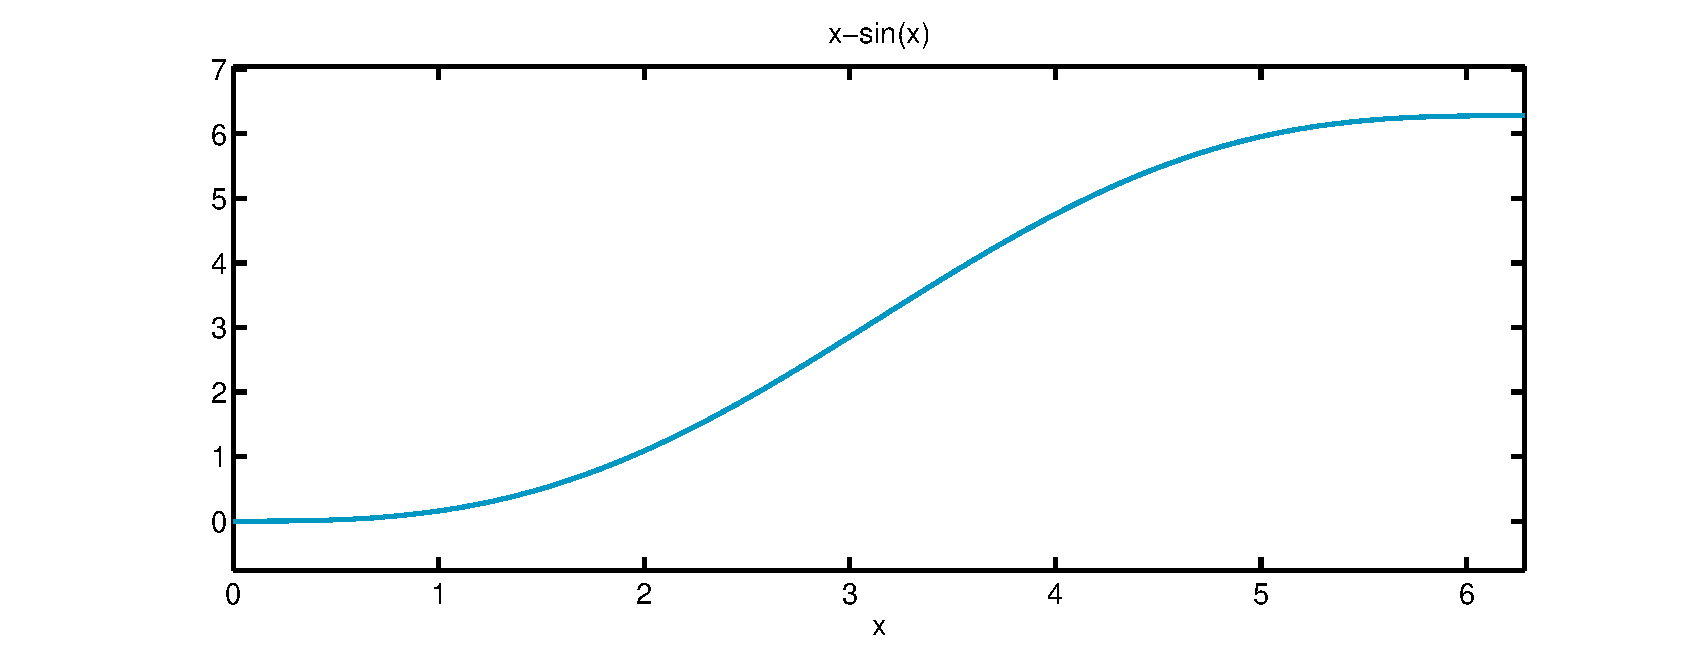
\includegraphics[width=0.5\textwidth]{show_ezplot-utc}}\\
%   Be careful with steep gradients: \lstinline$ezplot('x-sin(1/x)', [0 1])$% (use \lstinline$fplot$ instead)
%   \\
%   \centering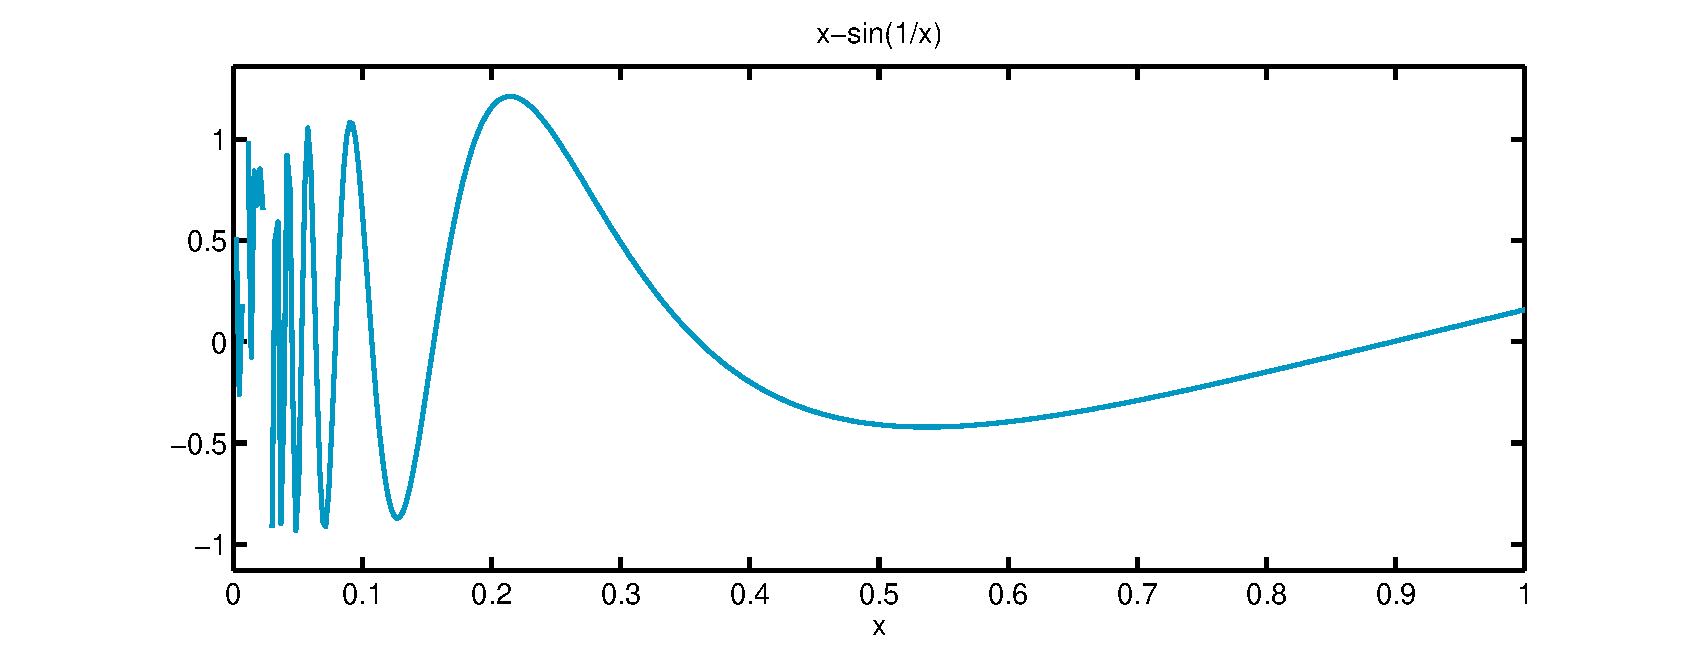
\includegraphics[width=0.5\textwidth]{show_ezplot2-utc}
% \end{frame}

\begin{frame}[fragile]
  \frametitle{Other plotting tools}
  \begin{columns}
   \column{0.6\textwidth}
    \begin{itemize}[<+->]
      \item Error bars: \lstinline$plt.errorbar(x, y, yerr=err)$
      \item 3D plots: \lstinline$ax.plot_trisurf(x, y, z)$
      \item Histograms: \lstinline$plt.hist(x, bins=20)$
    \end{itemize}
   \column{0.4\textwidth}
      \includegraphics<1>[width=\columnwidth]{show_errorbar-utc}
      \mode<presentation>{
        \includegraphics<2>[width=\columnwidth]{show_ezplot3-utc}
        \includegraphics<3>[width=\columnwidth]{show_hist-utc}
    }
 \end{columns}
\end{frame}

\subsection*{Multi-dimensional data}
\begin{frame}<handout:3>[fragile]
  \frametitle{Multi-dimensional data}
  Python typically requires the definition of rectangular grid coordinates using \lstinline$np.meshgrid$:\\
  \begin{overlayarea}{\textwidth}{6cm}
  \begin{columns}[T]
   \column{0.6\textwidth}
    \begin{lstlisting}[language=Python]
x, y = np.meshgrid(np.linspace(-2, 2, 41), np.linspace(-2, 2, 41))
z = x * y * np.exp(-x**2 - y**2)
    \end{lstlisting}
    \vskip1em
    \begin{itemize}
      \item<2-> Surface plot
      \item<3-> Contour plot
      \item<4-> Waterfall 
      \item<5> Ribbons
    \end{itemize}
   \column{0.4\textwidth}
   \begin{center}
      \includegraphics<2>[width=\columnwidth]{show_surf}
      \mode<presentation>{
        \includegraphics<3>[width=\columnwidth]{show_contour}
        \includegraphics<4>[width=\columnwidth]{show_waterfall}
        \includegraphics<5>[width=\columnwidth]{show_ribbon}
      }
   \end{center}
    \only<2>{
      \lstinline$ax.plot_surface(x, y, z)$
    }
    \mode<presentation>{
      \only<3>{
        \lstinline$v = np.linspace(-0.5, 0.5, 21)$\\
        \lstinline$cs = ax.contour(x, y, z, levels=v)$\\
        \lstinline$ax.clabel(cs, inline=1, fontsize=10)$
      }
      \only<4>{
      \lstinline$ax.plot_trisurf(x.flatten(), y.flatten(), z.flatten(), cmap='winter')$
      }
      \only<5>{
      \lstinline$ax.plot_trisurf(x.flatten(), y.flatten(), z.flatten(), cmap='viridis', linewidth=0, antialiased=False)$
      }
    }
 \end{columns}
 \end{overlayarea}
\end{frame}

\begin{frame}[fragile]
  \frametitle{Vector data}
  The gradient function, as expected, is used to obtain the gradient of a scalar field. Colors can be used in the background to simultaneously plot field data:
  \begin{columns}[T]
   \column{0.6\textwidth}
    \begin{lstlisting}[language=Python]
x, y = np.meshgrid(np.linspace(-2, 2, 21), np.linspace(-2, 2, 21))
z = x * y * np.exp(-x**2 - y**2)
dx, dy = np.gradient(z, 0.4, 0.4)

# Background
cs = plt.contourf(x, y, z, 30, cmap='hot')
plt.colorbar(cs)

plt.axis('tight')

# Vectors
plt.quiver(x, y, dx, dy, color='k')
    \end{lstlisting}
   \column{0.4\textwidth}
   \begin{center}
      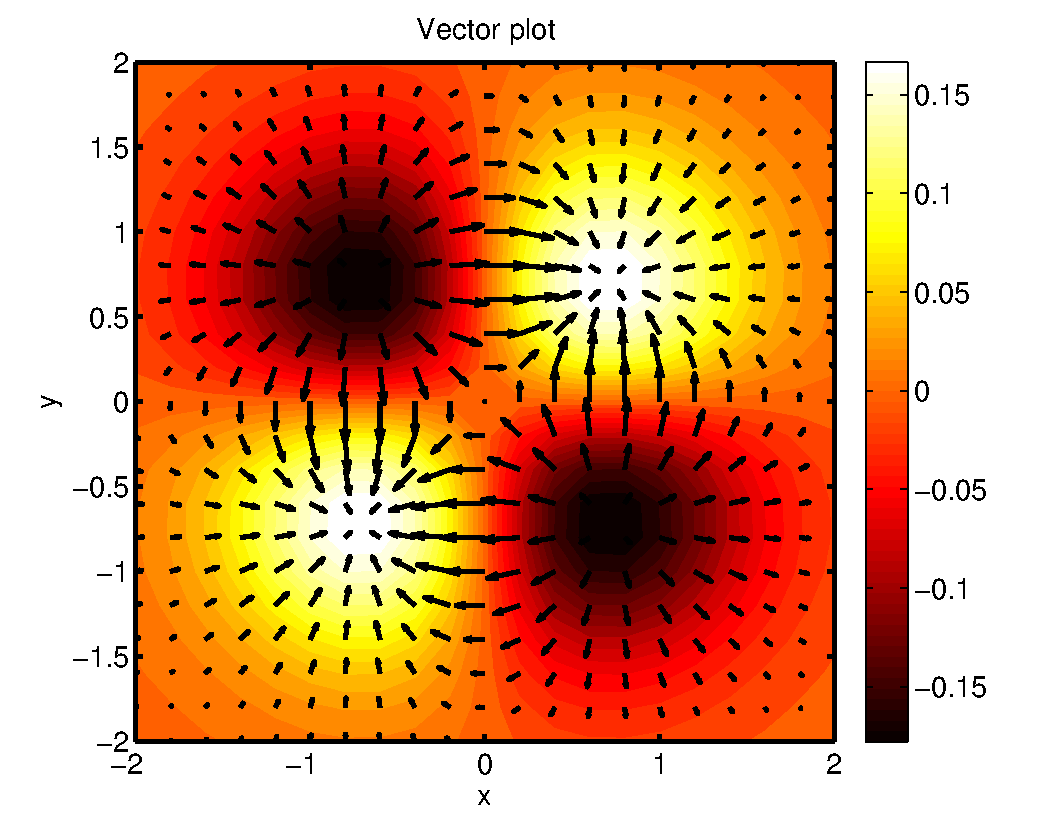
\includegraphics[width=\columnwidth]{show_vector}
    \end{center}
  \end{columns}
\end{frame}

\begin{frame}[fragile]
  \frametitle{Functions: revisited}
  In Python, you can define your own functions to re-use certain functionalities. We now define the mathematical function \(f = x^2+e^x\):
  \begin{lstlisting}[language=Python]
def f(x):
    import numpy as np
    return x**2 + np.exp(x)
  \end{lstlisting}
  \pause
  Note:
  \begin{itemize}
    \item The function is defined using the \lstinline[language=Python]|def| keyword.
    \item The variables used are \emph{local}. They will not be available globally unless defined as such.
    \item The function is defined in the Python script, not in a separate file.
    \item The function will work with NumPy arrays to handle vectorized inputs, returning an array of function values.
  \end{itemize}
\end{frame}


\begin{frame}[fragile]
  \frametitle{Inline functions}
  If you do not want to create a new function block, you can create an \emph{lambda function}:
  \begin{lstlisting}[language=Python]
f = lambda x: x**2 + np.exp(x)
  \end{lstlisting}
  \pause
  \begin{itemize}
    \item \lstinline[language=Python]|f|: the name of the function
    \item \lstinline[language=Python]|lambda|: used to define the inline function
    \item \lstinline[language=Python]|x|: the input argument
    \item \lstinline[language=Python]|x**2 + np.exp(x)|: the actual function
  \end{itemize}\pause
  \begin{lstlisting}[language=Python]
import numpy as np
f(np.linspace(0, 1, num=11))
  \end{lstlisting}
\end{frame}


\section{Concluding remarks}
\subsection*{Advanced}
\againframe<2>{contents_prog2}
\begin{frame}
  \frametitle{Advanced concepts}
  \begin{itemize}
    \item Object oriented programming: classes and objects
    \item Memory management: some programming languages require you to allocate computer memory yourself (e.g. for arrays)
    \item External libraries: in many cases, someone already built the general functionality you are looking for
    \item Compiling and scripting (``interpreted''); compiling means converting a program to computer-language before execution. Interpreted languages do this on the fly.
    \item Parallellization: Distributing expensive calculations over multiple processors or GPUs.
  \end{itemize}\pause
     \only<beamer>{
       \tikzstyle{every picture}-=[remember picture]
       \begin{tikzpicture}[remember picture,overlay]{
   \node at (current page.center) {
\includegraphics[width=\textwidth]{fullnerd2.png}};}
       \end{tikzpicture}}
 \end{frame}

\againframe{workrightfast}
\againframe{wrf-explain}

\subsection*{Exercise}
\begin{frame}<handout:1-2>
  \frametitle{Exercise: finding the roots of a parabola}
  We are writing a program that finds for us the roots of a parabola. We use the form
  \[
    y = ax^2 + bx + c
  \]
  \pause
  What is our program in pseudo-code? \pause
  \begin{enumerate}[<+->]
    \item Input data ($a$, $b$ and $c$)
    \item Identify special cases ($a=b=c=0$, $a=0$)
    \begin{description}
      \item[$a=b=c=0$] Solution indeterminate
      \item[$a=0$] Solution: $x = -\frac{c}{b}$
    \end{description}
    \item Find $D = b^2-4ac$
    \item Decide, based on $D$:
    \begin{description}
      \item[$D<0$] Display message: complex roots
      \item[$D=0$] Display 1 root value
      \item[$D>0$] Display 2 root values
    \end{description}
  \end{enumerate}
\end{frame}

\begin{frame}<handout:0>[plain,fragile]
  \frametitle{Example: finding the roots of a parabola}
  \small\selectfont
  \begin{lstlisting}[language=Python,basicstyle=\scriptsize\ttfamily]
def parabola(a, b, c):
    # Catch exception cases
    if a == 0:
        if b == 0:
            if c == 0:
                print('Solution indeterminate')
                return
            print('There is no solution')
            return
        return -c / b

    # Compute determinant
    D = b**2 - 4*a*c
    if D < 0:
        print('Complex roots')
        return
    elif D == 0:
        return -b / (2*a)
    elif D > 0:
        x1 = (-b + D**0.5) / (2*a)
        x2 = (-b - D**0.5) / (2*a)
        return sorted([x1, x2])
  \end{lstlisting}
\end{frame}

\begin{frame}[fragile]
  \frametitle{Example: finding the roots of a parabola}
  \begin{lstlisting}
>> parabola(1, -4, -3)
[-0.6457513110645907, 4.645751311064591]
  \end{lstlisting}
\end{frame}


%
%\subsection*{Projectile}
%\begin{frame}[fragile]
%\scriptsize\selectfont
%  \frametitle{Example: projectile trajectory}
%  \begin{center}
%    \begin{tikzpicture}[scale=0.7,ball/.style={circle,minimum size=8mm,thick,shading=ball,ball color=maincolor,
%				      font=\sffamily\scriptsize},>=stealth',thick,node distance=0.75cm]
%      \node[ball,anchor=north] (ball) at (0,0) {$M$};
%      \node[anchor=north east] at (1.5,1.7) (aim) {};
%      \node[anchor=south east] at (aim.south) {$v_0$};
%      \uncover<2->{\node at (7.5,-0.5) (aim2) {};
%      \node[anchor=north] at (aim2) {Trajectory};}    
%      \node at (4,2.6) (aim3) {};
%      \uncover<3->{\node[ball,ball color=gray,fill opacity=0.5] (ball2) at (aim3) {};}
%      
%      \draw[->] (ball.north east) -> (aim.center);
%      \draw<2->[->,dashed] (ball.north east) parabola bend (aim3) (aim2);
%      \draw<3->[->] (ball2) -- node[midway,anchor=west]{$F_g=mg$} ($ (ball2)+(0,-2) $);
%    \end{tikzpicture}
%  \end{center}
%  \vskip1em
%  \begin{itemize}
%    \item<1-> A ball with mass $M$ is thrown at time $t = 0$ with a certain velocity $v(t) = v(0) = v_0$
%    \item<2-> We need to describe the trajectory of the ball over time
%    \item<3-> It is given that the only force acting on the ball is gravity: $F = Mg$
%  \end{itemize}
%\end{frame}
%
%\begin{frame}[fragile]
%\scriptsize\selectfont
%  \frametitle{Example: projectile trajectory}
%  Computers cannot solve a continuous equation; we need to \emph{discretize} the time into steps of size $\Delta t$. Create a time line:\\ \vskip2em\pause
%  \begin{tikzpicture}[snake=zigzag, line before snake = 5mm, line after snake = 5mm]
%    %draw horizontal line   
%    \draw (0,0) -- (6,0);
%    \draw[snake] (5.5,0) -- (8.5,0);
%    \draw (8,0) -- (10,0);
%
%    %draw vertical lines
%    \foreach \x in {0,2,4,6,8,10}
%      \draw (\x cm,3pt) -- (\x cm,-3pt);
%
%    %draw nodes
%    \draw (0,0) node[below=3pt] {$ t=0 $} node[above=3pt] {$ 1 $};
%    \draw (2,0) node[below=3pt] {$ \Delta t $} node[above=3pt] {$ 2 $};
%    \draw (4,0) node[below=3pt] {$ 2\Delta t $} node[above=3pt] {$ 3 $};
%    \draw (6,0) node[below=3pt] {$ 3\Delta t $} node[above=3pt] {$ 4 $};
%    \draw (8,0) node[below=3pt] {$ t_\mathrm{end}-\Delta t $} node[above=3pt] {$ n-1 $};
%    \draw (10,0) node[below=3pt] {$ t_\mathrm{end} $} node[above=3pt] {$ n $};
%    
%    \onslide<4>{
%      \draw (0,-1.5) node[above=1pt] {$x_0$};
%      \draw (0,-1.5) node[below=3pt] {$v_0$};
%    }
%    \onslide<5>{
%      \draw (0,-1.5) node[above=1pt] {$x(t)$};
%      \draw (0,-1.5) node[below=3pt] {$v(t)$};
%      \draw (2,-1.5) node[above=1pt] {$x(t+\Delta t)$};
%      \draw (2,-1.5) node[below=3pt] {$v(t+\Delta t)$};
%    }
%    \onslide<6>{
%      \draw (2,-1.5) node[above=1pt] {$x(t)$};
%      \draw (2,-1.5) node[below=3pt] {$v(t)$};
%      \draw (4,-1.5) node[above=1pt] {$x(t+\Delta t)$};
%      \draw (4,-1.5) node[below=3pt] {$v(t+\Delta t)$};
%    }
%    \onslide<7>{
%      \draw (4,-1.5) node[above=1pt] {$x(t)$};
%      \draw (4,-1.5) node[below=3pt] {$v(t)$};
%      \draw (6,-1.5) node[above=1pt] {$x(t+\Delta t)$};
%      \draw (6,-1.5) node[below=3pt] {$v(t+\Delta t)$};
%    }
%   \end{tikzpicture}
%\end{frame}
%
%\begin{frame}[fragile]
%\scriptsize\selectfont
%  \frametitle{Example: projectile trajectory}
%  \begin{itemize}
%    \item A Taylor expansion shows how the $x$-position is obtained at discrete time intervals: 
%    \[ f(x) = f(a) + \frac{f'(a)}{1!}(x-a) + \frac{f''(a)}{2!}(x-a)^2  + \ldots \]\pause
%    \[ x(t+\Delta t) = x(t) + \frac{\frac{dx}{dt}(t)}{1!}(t + \Delta t - t) + \frac{\frac{d^2x}{dt^2}}{2!}(t+\Delta t - t)^2  + O(\Delta t^3) \] \pause
%    \[ x(t+\Delta t) = x(t) + v(t)\Delta t + \frac{F}{2M}\Delta t^2  + O(\Delta t^3) \] \pause
%    \item Taking small time steps, we can discard $\Delta t^2$ and subsequent terms:
%    \[ x(t+\Delta t) = x(t) + v(t)\Delta t \] \pause
%    \item A similar approach is taken for the velocity:
%    \[ v(t+\Delta t) = v(t) + a(t)\Delta t \] \pause
%    \[ F = Ma \Rightarrow a = \frac{F}{M} \Rightarrow v(t+\Delta t) = v(t) + \frac{F(t)}{M}\Delta t \]
%  \end{itemize}
%\end{frame}
%
%\begin{frame}[fragile]
%\scriptsize\selectfont
%  \frametitle{Example: projectile trajectory}
%  Our mathematical model is as follows: \pause
%  \begin{enumerate}
%    \item Initialisation of parameters ($x_0$, $v_0$, $g$, $\Delta t$, $t_end$, $M$)\pause
%    \item Create storage vectors for time, position, velocity \pause
%    \item Start a time-marching loop \pause
%    \begin{itemize}
%    \scriptsize\selectfont
%      \item Calculate $x(t+\Delta t)$, then $F$, then $v(t+\Delta t)$:
%      \[ x(t+\Delta t) = x(t) + v(t)\Delta t \] 
%      \[ F = Mg \]
%      \[ v(t+\Delta t) = v(t) + \frac{F}{M}\Delta t \] \pause
%      \item Store current solution
%    \end{itemize}
%    \item Draw result and return solution vector $x$
%    \begin{itemize}
%      \item Exact solution:
%      \[
%        x(t) = x_0 + v_0 t + ( \frac{1}{2} -9.81 t^2 )
%      \]
%    \end{itemize}
%  \end{enumerate}
%\end{frame}
%
%\begin{frame}[fragile]
%  \frametitle{Example: projectile trajectory - solution (initialisation)}
%  \scriptsize\selectfont
%  \begin{lstlisting}
%function [pos,tim] = projectile(v0,M)
%
%% Initialise parameters
%t_end = 2;                  % End time
%deltat = 0.01;              % Time step
%x0 = 1;                     % Initial position
%
%nsteps = fix(t_end/deltat); % Number of time steps
%pos = zeros(nsteps,1);      % Position vector
%vel = zeros(nsteps,1);      % Velocity vector
%tim = zeros(nsteps,1);      % Time vector
%
%% Default values for mass and velocity
%if (nargin < 2)
%    M = 10;
%    if (nargin < 1)
%        v0 = 1;
%    end
%end
%  \end{lstlisting}
%\end{frame}
%
%\begin{frame}[fragile]
%  \frametitle{Example: projectile trajectory - solution (main program)}
%  \scriptsize\selectfont
%  \begin{lstlisting}
%pos(1) = x0;                % Store initial position
%vel(1) = v0;                % Store initial velocity
%
%% The time loop
%for n = 1:nsteps-1
%    pos(n+1) = position(pos(n),vel(n),deltat);
%    vel(n+1) = velocity(vel(n),M,deltat);
%    tim(n+1) = tim(n) + deltat;
%end
%
%% Plot results
%figure; plot(tim,pos, 'o');
%
%% Compare to analytical solution
%compareToExact(x0,v0,tim,pos);
%
%end
%  \end{lstlisting}
%\end{frame}
%
%\begin{frame}[fragile]
%  \frametitle{Example: projectile trajectory - solution (added functions)}
%  \scriptsize\selectfont
%  \begin{lstlisting}
%function F = force(M)
%% M:    mass of particle
%g = -9.81;
%F = M * g;
%end
%
%function v = velocity(vt,mass,dt)
%% vt:   velocity at previous time
%% mass: mass of particle
%% dt:   time step size
%v = vt + force(mass)/mass * dt;
%end
%
%function x = position(xt,vel,dt)
%% xt:   position at current time step
%% vel:  velocity at current time step
%% dt:   time step size
%x = xt + vel * dt;
%end
%  \end{lstlisting}
%\end{frame}
%
%\begin{frame}[fragile]
%  \frametitle{Example: projectile trajectory - solution (verification)}
%  \scriptsize\selectfont
%  \begin{lstlisting}
%function compareToExact(x0,v0,tim,pos)
%
%% Exact solution
%pos_ex = x0 + v0 * tim + ( 0.5 * -9.81 * tim .* tim );
%
%% Draw comparative figure
%figure;
%subplot(2,1,1)
%plot(tim,pos, 'o');
%hold on;
%plot(tim,pos_ex,'r-')
%subplot(2,1,2)
%stem(tim,pos_ex-pos,'r-')
%
%% Print the L2-error norm
%norm(pos_ex - pos)
%end
%  \end{lstlisting}
%\end{frame}
%
%\begin{frame}
%  \frametitle{Example: projectile trajectory - solution}
%  \begin{center}
%    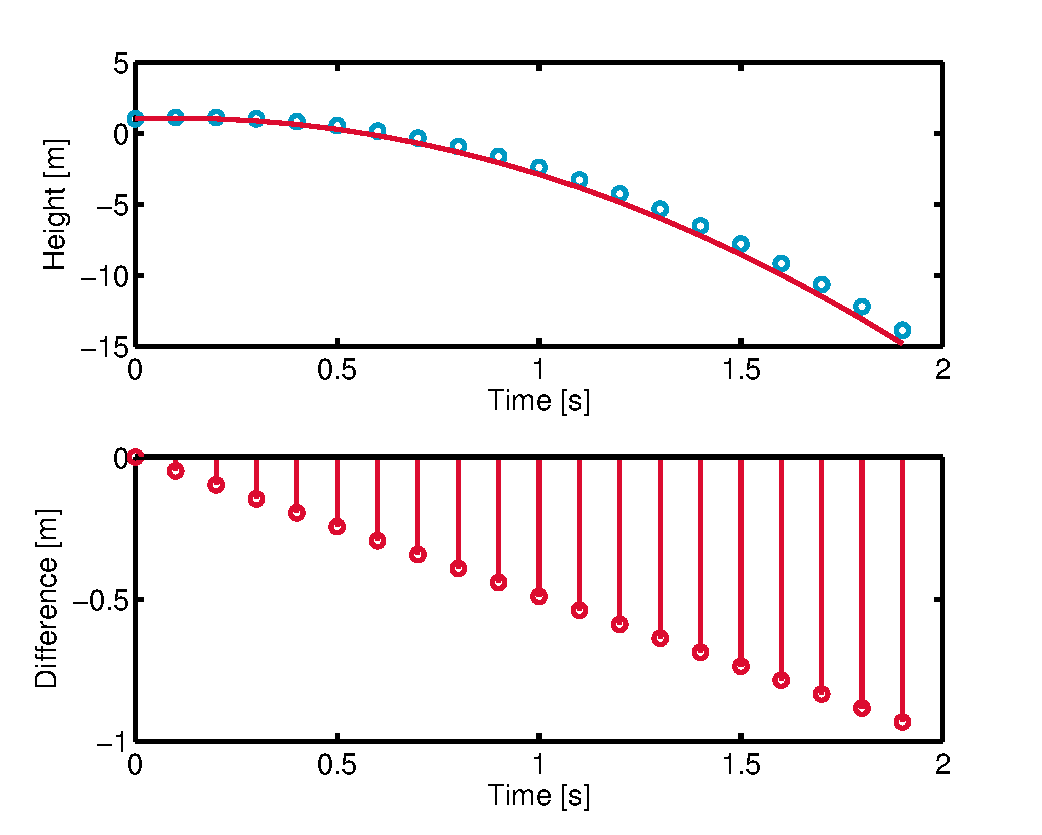
\includegraphics[width=0.8\textwidth]{projectile-utc}
%  \end{center}
%\end{frame}

\title{Numerical errors in computer simulations}
\subtitle{}
\lecture{Numerical errors}{numericalerrors}
\section{Introduction}
\subsection*{General}
\begin{frame}[label=contents_err]
  \frametitle{Today's outline}
  \mode<beamer>{
    \only<1>{\tableofcontents}
  }
  \only<2>{\tableofcontents[currentsection,currentsubsection]}
\end{frame}

% \begin{frame}
%  \frametitle{Errors in computer programs}
%   In the previous lecture, we have identified three error categories in programming:
%   \begin{description}
%    \item[Syntax errors] You did not obey the language rules. These errors prevent running or compilation of the program.
%    \item[Runtime errors] Something goes wrong during the execution of the program resulting in an error message (problem with input, division by zero, loading of non-existent files, memory problems, etc.)
%    \item[Semantic errors] The program does not do what you expect, but does what have told it to do.
%   \end{description}
%   \pause
%   This is only a subset of all errors that may be encountered:
%   \begin{description}
%    \item[Mathematical model errors] The equations do not describe the physical system
%    \item[Implementation errors] Includes the errors given above
%    \item[Numerical errors] Roundoff, truncation and break errors
%   \end{description}
% \end{frame}

\subsection*{Numerical errors}
\frame{
  \frametitle{Example 1}
  Start your spreadsheet program (Excel, ...) \vskip2em \pause 
  \begin{columns}[T]
    \column{0.5\textwidth}
    Enter: \vskip1em 
    \begin{tabular}{l!{\vrule}c}
        Cell   & Value   \\ \hline
        A1     & \texttt{0.1} \pause \\
        A2     & \texttt{=(A1*10)-0.9} \pause\\
        A3     & \texttt{=(A2*10)-0.9} \pause\\
        A4     & \texttt{=(A3*10)-0.9}
    \end{tabular} \\
    \vskip2em
    (repeat until A30)
    \pause \vskip1em What's happening? \pause

    \column{0.5\textwidth}
    Enter: \vskip1em 
    \begin{tabular}{l!{\vrule}c}
        Cell   & Value  \\ \hline
        A1     & \texttt{2} \pause \\
        A2     & \texttt{=(A1*10)-18}\\
        A3     & \texttt{=(A2*10)-18}\\
        A4     & \texttt{=(A3*10)-18}\\
    \end{tabular}  \\ 
    \vskip2em
    (repeat until A30)
  \end{columns}
}

\begin{frame}[fragile]
  \frametitle{Example 2}
    Start Matlab \vskip2em \pause 
    Investigate the result of \lstinline$sin(1e40 * pi)$ \vskip2em \pause
    Create a vector \lstinline$v$ containing the powers of 10, e.g. from $10^0$ up to $10^{40}$ and solve \lstinline$sin(v * pi)$:
    \begin{lstlisting}
v = logspace(0,40,41);
y = sin(v*pi);
loglog(v,abs(y));     % Double log plot, values on y-axis must be positive.
    \end{lstlisting}
\end{frame}

\begin{frame}<1-2>[label=errors]
  \frametitle{Errors in computer simulations}
  In this course we will outline different numerical errors that may appear in computer simulations, and how these errors can affect the simulation results.
  \vskip2em
  \pause
  \begin{itemize}[<+->]
  \item Errors in the mathematical model (physics) % Wordt hier niet behandeld, zie FTV/CRE 
  \item Errors in the program (implementation)     % Is behandeld in eerste deel college (bij gebruik debugger)
  \item Errors in the entered parameters           % Wordt hier niet behandeld, zie practicum PT
  \item\alert<7>{ Roundoff- and truncation errors} % Wordt hier behandeld
  \item\alert<7>{ Break errors}                           % Wordt hier behandeld
  \end{itemize}
\end{frame}

\begin{frame}<1-3>[label=verification,fragile]
 \frametitle{Verification and validation}
  \scriptsize\selectfont
  \begin{columns}
    \column{0.6\textwidth}
    \uncover<3->{\begin{block}{Verification}
    Verification is the process of mathematically and computationally assuring that the model computes what you have entered.    
    \end{block}
    }
    \uncover<7->{
    \begin{block}{Validation}
      Validation is the process of determining the degree to which a model is an accurate representation of the real world from the perspective of the intended uses of the model
    \end{block}
    }

  \column{0.4\textwidth}
    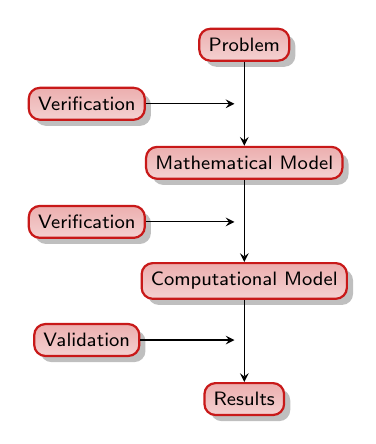
\begin{tikzpicture}[block/.style={rectangle,minimum size=3mm,text badly centered,drop shadow,
					thick,rounded corners,draw=maincolor,top color=maincolor!35,bottom color=maincolor!20,
					font=\sffamily\scriptsize},>=stealth,node distance=0.75cm]
	\node[block] (p) at (0,0) {Problem};
	\uncover<2->{\node[below of=p] (p1) {};
	\node[block, below of=p1] (mm) {Mathematical Model};
	\node[below of=mm] (mm1) {};}
	\uncover<4->{\node[block, below of=mm1] (cm) {Computational Model};
	\node[below of=cm] (cm1) {};}
	\uncover<6->{\node[block, below of=cm1] (r) {Results};}
	
	\uncover<3->{\node[block, left of=p1,node distance=2cm] (v1) {Verification};}
	\uncover<5->{\node[block, left of=mm1,node distance=2cm] (v2) {Verification};}
	\uncover<7->{\node[block, left of=cm1,node distance=2cm] (v3) {Validation};}
	
	\uncover<2->{\draw[->] (p) -> (mm);}
	\uncover<4->{\draw[->] (mm) -> (cm);}
	\uncover<6->{\draw[->] (cm) -> (r);}
	
	\uncover<3->{\draw[->] (v1) -> (p1);}
	\uncover<5->{\draw[->] (v2) -> (mm1);}
	\uncover<7->{\draw[->] (v3) -> (cm1);}
    \end{tikzpicture}
  \end{columns}
\end{frame}
% 

\begin{frame}
  \frametitle{Verification of the physical model}
  \scriptsize\selectfont
  \begin{columns}
    \column{0.5\textwidth}
    \begin{center}
      \mode<beamer>{
	\includegraphics<1>[width=0.7\columnwidth]{ptolemy1-1}
	\includegraphics<2>[width=0.7\columnwidth]{ptolemy1-2}
	\includegraphics<3>[width=0.7\columnwidth]{ptolemy1-3}
	\includegraphics<4>[width=0.7\columnwidth]{ptolemy1-4}
	\includegraphics<5>[width=0.7\columnwidth]{ptolemy1-5}
	\includegraphics<6>[width=0.7\columnwidth]{ptolemy1-6}
      }
      \includegraphics<7->[width=0.7\columnwidth]{ptolemy1-7}
    \end{center}
    \column{0.5\textwidth}
    \begin{center}
      \mode<beamer>{
	\includegraphics<7>[width=0.7\columnwidth]{ptolemy2-0}
	\includegraphics<8>[width=0.7\columnwidth]{ptolemy2-1}
	\includegraphics<9>[width=0.7\columnwidth]{ptolemy2-2}
	\includegraphics<10>[width=0.7\columnwidth]{ptolemy2-3}
	\includegraphics<11>[width=0.7\columnwidth]{ptolemy2-4}
	\includegraphics<12>[width=0.7\columnwidth]{ptolemy2-5}
	\includegraphics<13>[width=0.7\columnwidth]{ptolemy2-6}
      }
      \includegraphics<14>[width=0.7\columnwidth]{ptolemy2-7}
    \end{center}
  \end{columns}
  \begin{itemize}
    \item<7-> The perceived orbit of Mars from Earth shows a zig-zag (in contrast to the Sun, Mercury, Venus)
    \item<14> Even though they were not 'right', Earth-centered models (Ptolemy) were still valid
  \end{itemize}
\end{frame}

\begin{frame}
  \frametitle{Be aware of your uncertainties}
  \vfill
  \begin{block}{Aleatory uncertainty}
    Uncertainty that arises due to inherent randomness of the system, features that are too complex to measure and take into account
  \end{block}
  \vskip1em
  \begin{block}{Epistemic uncertainty}
      Uncertainty that arises due to lack of knowledge of the system, but could in principle be known
  \end{block}
  \vfill
\end{frame}

\againframe<2-3>{errors}
\againframe<3-5>{verification}
\againframe<3-4>{errors}
\againframe<5-7>{verification}
\againframe<4->{errors}

\subsection*{Significant digits}
\frame{ 
  \frametitle{Significant digits}
  A numerical result $\tilde{x}$ is an approximation of the real value $x$.
  \begin{itemize}
  \colorize<1>  \item Absolute error
    \[ \delta = \lvert\tilde{x} - x\rvert, x \neq 0 \]
  \colorize<2>  \item Relative error
    \[ \frac{\delta}{\tilde{x}} = \lvert\frac{\tilde{x} - x}{\tilde{x}}\rvert \]
  \colorize<3> \item Error margin 
    \[ \tilde{x} - \delta \leq x \leq \tilde{x} + \delta \] 
    \[ x = \tilde{x} \pm \delta \]
  \end{itemize}
}

\frame{ 
  \frametitle{Significant digits}
  \begin{itemize}
   \colorize<1> \item $\tilde{x}$ has $m$ significant digits if the absolute error in $x$ is smaller or equal to 5 at the $(m+1)$-th position:
   \[ 10^{q-1} \leq \abs{\tilde{x}} \leq 10^q \]
   \[\abs{x-\tilde{x}} = 0.5 \times 10^{q-m}\]
   \colorize<2> \item For example:
   \[ x = \frac{1}{3}, \tilde{x} = 0.333 \Rightarrow \delta = 0.00033333\ldots \]
   3 significant digits
  \end{itemize}
}

\section{Roundoff and truncation errors}
\againframe<2>{contents_err}
\subsection*{roundoff}
\frame{
 \frametitle{Representation of numbers}
 \begin{itemize}[<+->]
  \item Computers represent a number with a finite number of digits: each number is therefore an approximation due to roundoff and truncation errors.
  \item In the decimal system, a digit $c$ at position $n$ has a value of $c \times 10^{n-1}$
 \end{itemize}
 \pause
  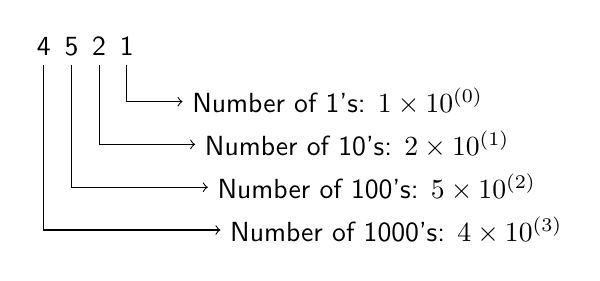
\begin{tikzpicture}[->]
  \node (A) {4};
  \node [right of = A,node distance=10pt] (B) {5};
  \node [right of = B,node distance=10pt] (C) {2};
  \node [right of = C,node distance=10pt] (D) {1};
  
  \node [below right of = D,node distance=1cm,anchor=west] (DD) {Number of 1's: $1 \times 10^{(0)}$};
  \node [below right of = DD,node distance=10pt,anchor=north] (CC) {Number of 10's: $2 \times 10^{(1)}$};
  \node [below right of = CC,node distance=10pt,anchor=north] (BB) {Number of 100's: $5 \times 10^{(2)}$};
  \node [below right of = BB,node distance=10pt,anchor=north] (AA) {Number of 1000's: $4 \times 10^{(3)}$};
  
  \draw (D) |- (DD);
  \draw (C) |- (CC);
  \draw (B) |- (BB);
  \draw (A) |- (AA);
  \end{tikzpicture}
  \pause
  \[ (4521)_{10} = 4 \times 10^3 + 5\times 10^2 + 2 \times 10^1 + 1 \times 10^0 \]
}

% \frame{
%  \frametitle{Representation of numbers}
%  \begin{itemize}[<+->]
%   \item You could use another basis, computers often use the basis 2:
%   \begin{align*}   
%   \hspace*{-1cm}
%  (4521)_{10} = 1& \times 2^{12} + 0 \times 2^{11} + 0 \times 2^{10} + 0 \times 2^9 + 1 \times 2^8 + \ldots \\ 
%   \ldots 1& \times 2^7 + 0 \times 2^6 + 1 \times 2^5 + 0 \times 2^4 + \ldots \\
%   \ldots 1& \times 2^3 + 0 \times 2^2 + 0 \times 2^1 + 1 \times 2^0 \\
%   =& (1000110101001)_2
%   \end{align*}
%   \item In general: 
%   \[ (c_m \ldots c_1 c_0)_q = c_0q^0 + c_1q^1 + \ldots + c_mq^m, c\in\left\{0,1,2,\ldots,q-1\right\} \]
%  \end{itemize}
% }

\frame{
 \frametitle{Representation of numbers}
 \begin{itemize}[<+->]
  \item You could use another basis, computers often use the basis 2:
  \begin{align*}   
  \hspace*{-1cm}
 (4521)_{10} = \onslide<2->{1& \times 2^{12} + \onslide<3->{0 \times 2^{11} + \onslide<4->{0 \times 2^{10} + \onslide<5->{0 \times 2^9 + \onslide<6->{1 \times 2^8 + \ldots \\ 
  \onslide<7->{\ldots 1& \times 2^7 + \onslide<8->{0 \times 2^6 + \onslide<9->{1 \times 2^5 + \onslide<10->{0 \times 2^4 + \ldots \\
  \onslide<11->{\ldots 1& \times 2^3 + \onslide<12->{0 \times 2^2 + \onslide<13->{0 \times 2^1 + \onslide<14->{1 \times 2^0}}}}}}}}}}}}} \\
  =& (\onslide<2->{1\onslide<3->{0\onslide<4->{0\onslide<5->{0\onslide<6->{1\onslide<7->{1\onslide<8->{0\onslide<9->{1\onslide<10->{0\onslide<11->{1\onslide<12->{0\onslide<13->{0\onslide<14->{1)_2}}}}}}}}}}}}}
  \end{align*}
  \onslide<15->{
  \item In general: 
  \[ (c_m \ldots c_1 c_0)_q = c_0q^0 + c_1q^1 + \ldots + c_mq^m, c\in\left\{0,1,2,\ldots,q-1\right\} \]
  }
 \end{itemize}
}

\frame{
 \frametitle{Representation of numbers}
 \begin{itemize}
  \colorize<1> \item Numbers are stored in binary in the memory of a computer, in segments of a specific length (called a \emph{word}).
  \colorize<2> \item We distinguish multiple types of numbers:
  \begin{itemize}
   \colorize<2> \item Integers: $-301, -1, 0, 1, 96, 2293, \ldots$
   \colorize<2> \item Floating points: $-301.01, 0.01, 3.14159265, 14498.2$
  \end{itemize}
  \colorize<3> \item A binary integer representation looks like the following bit sequence:
  \[ z = \sigma \left( c_02^0 + c_12^1 + \ldots + c_{\lambda-1}2^{\lambda-1}\right) \]
  $\sigma$ is the sign of $z$ (+ or -), and $\lambda$ is the length of the word
  \colorize<4> \item Endianness: the order of bits stored by a computer
 \end{itemize}
}

\frame{
 \frametitle{Excercise}
 \begin{itemize}
  \item Convert the following decimal number to base-2: 214 \pause
  \[ 214_{10} = 11010110_2 \] \pause
   \item Excel: 
   \begin{itemize}
     \item Decimal: \texttt{=DEC2BIN(214)}
     \item Octal: \texttt{=DEC2OCT(214)}
     \item Hexadecimal: \texttt{=DEC2HEX(214)}
   \end{itemize}\pause
   \item Matlab: 
   \begin{itemize}
    \item Decimal: \lstinline$dec2bin(214)$
    \item Other base: \lstinline$dec2base(214,<base>)$
    \end{itemize}
 \end{itemize}
}

\begin{frame}
  \frametitle{Arithmetic operations with binary numbers}
  \centering 
  Addition: \vskip1em
  \begin{columns}
  \column{0.2\textwidth}
    $ 0 + 0 = 0$\\
    $ 0 + 1 = 1$\\
    $ 1 + 0 = 1$\\
    \alert{$ 1 + 1 = 0$ (carry one)}\pause
    \column{0.3\textwidth}
      \begin{tabular}{cccc}
	  & 1 & 4 & 5 \\
	+ &   & 2 & 3 \\
	\hline
	  & 1 & 6 & 8 \\
      \end{tabular}\pause
    \column{0.5\textwidth}
      \begin{tabular}{ccccccccc}
	  & 1 & 0 & 0 & 1 & 0 & 0 & 0 & 1\\
	+ & 0 & 0 & 0 & 1 & 0 & 1 & 1 & 1 \\
	\hline \pause
	  & 1 & 0 & 1 & 0 & 1 & 0 & 0 & 0 \\
      \end{tabular}
  \end{columns}
  \pause
\centering 
  Subtraction: \\ \vskip1em
  \begin{columns}
  \column{0.2\textwidth}
    $ 0 - 0 = 0$\\
    $1 - 0 = 1$\\
    $1 - 1 = 0$\\
    \alert{$0 - 1 = 1$ (borrow one)}\pause
    \column{0.3\textwidth}
      \begin{tabular}{cccc}
	  & 1 & 4 & 5 \\
	- &   & 2 & 3 \\
	\hline
	  & 1 & 2 & 2 \\
      \end{tabular}\pause
    \column{0.5\textwidth}
      \begin{tabular}{ccccccccc}
	  & 1 & 0 & 0 & 1 & 0 & 0 & 0 & 1\\
	- & 0 & 0 & 0 & 1 & 0 & 1 & 1 & 1 \\
	\hline \pause
	  & 0 & 1 & 1 & 1 & 1 & 0 & 1 & 0 \\
      \end{tabular}
  \end{columns}
  \begin{itemize}
    \item Multiplication and division are more expensive, and more elaborate
  \end{itemize}
\end{frame}

\frame{
 \frametitle{Excercise}
  Try the following commands in Matlab:
    \begin{longtable}{l!{\vrule}c}
      Command & Result \\ \hline
      \texttt{intmin}   & \texttt{-2147483648} \pause \\
      \texttt{intmax}   & \texttt{2147483647} \pause\\
      \texttt{i = int16(intmax)}   & \texttt{i = 32767} \pause\\
      \texttt{whos i}   & \texttt{int16} information \pause\\
      \texttt{i = i + 100}& \texttt{i = 32767} \pause\\
      \texttt{realmax  }& \texttt{1.7977e+308} \pause\\
      \texttt{f = 0.1}& \pause\\
      \texttt{whos f}   & \texttt{double} information \pause\\
      \texttt{format long e} & \pause\\
      \texttt{realmax  }& \texttt{1.797693134862316e+308} \pause\\
      \texttt{f}& \pause\\
      \texttt{fprintf("\%0.16f",f)}& \texttt{0.1000000000000000} \pause\\
      \texttt{fprintf("\%0.20f",f)}& \texttt{0.10000000000000000555}
    \end{longtable}
}

\frame{
 \frametitle{Representation of integer numbers}
  \begin{itemize}[<+->]
   \item In Matlab, integers of the type \lstinline$int32$ are represented by 32-bit words ($\lambda = 31$).
   \item The set of numbers that an \lstinline$int32$ $z$ can represent is:
   \[ -2^{31} \leq z \leq 2^{31} - 1 \approx 2\times 10^{9} \]
   \item If, during a calculation, an integer number becomes larger than $2^\lambda-1$, the computer reports an \alert{overflow}\footnote{Matlab does not perform actual integer overflows, it just stops at the maximum.}
   \item How can a computer identify an overflow?
  \end{itemize}
}

\begin{frame}[fragile]
 \frametitle{Representation of real (floating point) numbers}
 \begin{itemize}
    \item Formally, a real number is represented by the following bit sequence
    \[ x = \sigma \left( 2^{-1} + c_2 2^{-2} + \ldots + c_m 2^{-m} \right)2^{e-1023} \] \\
    Here, $\sigma$ is  the sign of $x$ and $e$ is an integer value.
  \item A floating point number hence contains sections that contain the sign, the exponent and the mantissa \\
  \vskip1em
    \centering
    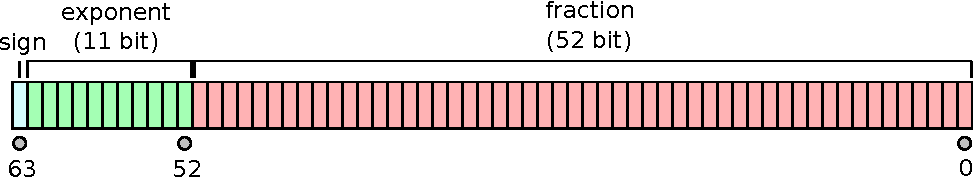
\includegraphics[width=0.9\textwidth]{IEEE_754_Double_Floating_Point_Format}
    \begin{flushright}
    {\tiny
    Image: \href{http://commons.wikimedia.org/wiki/File:IEEE_754_Double_Floating_Point_Format.svg#mediaviewer/File:IEEE_754_Double_Floating_Point_Format.svg}{Wikimedia Commons CC by-SA}} 
    \end{flushright}
 \end{itemize}
\end{frame}

\begin{frame}[fragile]
 \frametitle{Representation of real (floating point) numbers}
 \begin{itemize}
    \item Example: $\lambda = 3$, $m = 2$, $x = \frac{2}{3}$
    \[ x = \pm \left( 2^{-1} + c_2 2^{-2}\right)2^e \]
    \begin{itemize}
      \item $c_0 \in \{0,1\}$
      \item $e = \pm a_0 2^0$
      \item $a_0 \in \{0,1\}$
    \end{itemize}
    \item Truncation: $fl(x) = 2^{-1} = 0.5$
    \item Round off: $fl(x) = 2^{-1} + 2^{-2} = 0.75$
 \end{itemize}
\end{frame}

% \begin{frame}[fragile]
%  \frametitle{Representation of floating point numbers}
%  \begin{columns}
%  \column{0.6\textwidth}
%   \begin{itemize}
%     \item A double is 64 bits (8 bytes)
%     \item Calculate the size of $s$
%     \[ s = \sum_{m=0}^{63} 2^m \onslide<3->{= 1.8447e+19} \]
%   \end{itemize}
%   \pause 
%  \column{0.4\textwidth}
%  \begin{block}{Code example}
%   \begin{lstlisting}
% s = 0;
% for i = 0:63
% s = s + 2^i;
% end
% s
%   \end{lstlisting}
%  \end{block}
%  \pause 
%  \end{columns}
%   \pause
%  \begin{itemize}
%   \item Why is this number smaller than \lstinline$realmax$?
%  \end{itemize}
%  \pause
%  \centering
%  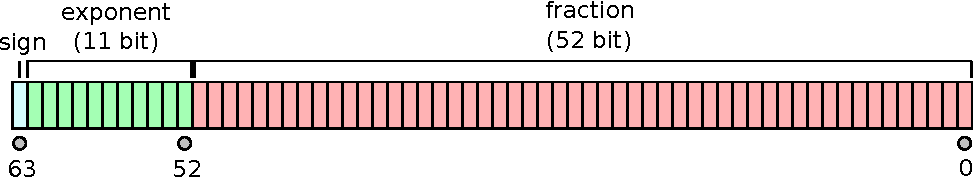
\includegraphics[width=0.9\textwidth]{IEEE_754_Double_Floating_Point_Format}
%    \begin{flushright}
%   {\tiny
%    Image: \href{http://commons.wikimedia.org/wiki/File:IEEE_754_Double_Floating_Point_Format.svg#mediaviewer/File:IEEE_754_Double_Floating_Point_Format.svg}{Wikimedia Commons}} CCA by-SA
%   \end{flushright}
% \end{frame}

\section{Break errors}
\againframe<2>{contents_err}
\subsection*{break}
\begin{frame}
   \frametitle{Trigonometric, Logarithmic, and Exponential computations}
    \begin{itemize}
     \colorize<1> \item Processors can do logic and arithmetic instructions
     \colorize<2> \item Trigonometric, logarithmic and exponential calculations are ``higher-level'' functions:\\
      $\exp$, $\sin$, $\cos$, $\tan$, $\sec$, $\arcsin$, $\arccos$, $\arctan$, $\log$, $\ln$, $\ldots$
      \colorize<3> \item Such functions can be performed using these ``low level'' instructions, for instance using a Taylor series:
      \begin{align*}
        \sin(x) &= \sum_{n=0}^{\infty} \frac{(-1)^n}{(2n+1)!}x^{2n+1} =  x - \frac{x^3}{3!} + \frac{x^5}{5!} - \frac{x^7}{7!} + \ldots \\
         e^x &= \sum_{n=0}^\infty \frac{x^n}{x!} = 1 + x + \frac{x^2}{2!} + \frac{x^3}{3!} + \frac{x^4}{4!} + \ldots
      \end{align*}
    \end{itemize}
\end{frame}

\begin{frame}
   \frametitle{Trigonometric, Logarithmic, and Exponential computations}
    \begin{itemize}
      \colorize<1> \item These operations involve many multiplications and additions, and are therefore \emph{expensive}
      \colorize<2> \item Computations can only take finite time, for infinite series, calculations are interrupted at $N$
    \end{itemize}
%     \hspace*{-2cm} 
    \colorize<2> \begin{flalign*}
      \sin(x) &= \sum_{n=0}^N \frac{(-1)^n}{(2n+1)!}x^{2n+1} =  x - \frac{x^3}{3!} + \frac{x^5}{5!} - \ldots + \frac{(-1)^N}{(2N+1)!}x^{2N+1} & \\
          e^x &= \sum_{n=0}^N \frac{x^n}{x!} = 1 + x + \frac{x^2}{2!} + \frac{x^3}{3!} + \frac{x^4}{4!} + \ldots + \frac{x^N}{N!} &
    \end{flalign*}
    \begin{itemize}
      \colorize<3> \item This results in a \emph{break error}
    \end{itemize}
\end{frame}

\begin{frame}
  \frametitle{Algorithm for sine-computation}
  A computer may use a clever algorithm to limit the number of operations required to perform a higher-level function. A (fictional!) example for the computation of $\sin(x)$:\\
  \begin{columns}
    \column{0.5\textwidth}
    \begin{enumerate}[<+->]
      \item<2-> Use periodicity so that $0 \leq x \leq 2\pi$
      \item<3-> Use symmetry ($0\leq x \leq \frac{\pi}{2}$)
      \item<4-> Use lookup tables for known values
      \item<5-> Perform taylor expansion
    \end{enumerate}

    \column{0.5\textwidth}
    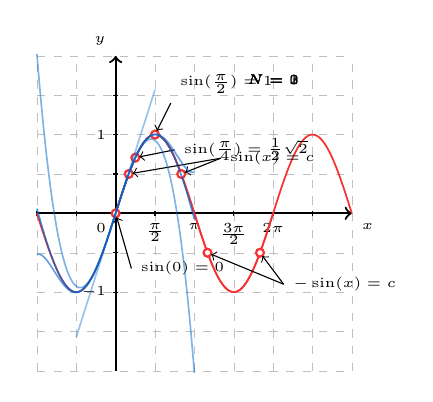
\begin{tikzpicture}[font=\tiny]
      % Grid
      \draw[gridline,step=0.5] (-1,-2) grid (3,2);
      % Axes
      \draw[thick,->] (-1,0) -- (3,0) node[anchor=north west] {$x$};
      \draw[thick,->] (0,-2) -- (0,2) node[anchor=south east] {$y$};
      % Ticks
      \foreach \x in {-1,-0.5,...,2.5}
	\draw (\x cm,1pt) -- (\x cm,-1pt) node[anchor=north] {};
      \foreach \y in {-1,-0.5,...,1.5}
	\draw (1pt,\y cm) -- (-1pt,\y cm) node[anchor=east] {};
      % Ticks (labels)
      \node [anchor=north east] (0,0) {$0$};
      \node [anchor=north ] at (0.5,0) {$\frac{\pi}{2}$};
      \node [anchor=north ] at (1  ,0) {$\pi$};
      \node [anchor=north ] at (1.5,0) {$\frac{3\pi}{2}$};
      \node [anchor=north ] at (2,0) {$2\pi$};
      \node [anchor=east] at (0,-1) {$-1$};
      \node [anchor=east] at (0,1) {$1$};
      % Full graph
      \draw<1> [graph,domain=-1:3] plot (\x, {sin(\x * pi r)});
      % Periodicity
      \draw<2-> [graph,opacity=0.2,domain=-1:3] plot (\x, {sin(\x * pi r)});
      \draw<2> [graph,domain=0:2] plot (\x, {sin(\x * pi r)});
      % Symmetry
      \draw<3-> [graph,domain=0:0.5] plot (\x, {sin(\x * pi r)});
      \node<3> [dot] at (1.8333,-0.5) (c1) {};
      \node<3> [dot] at (1.1667,-0.5) (c2) {};
      \draw<3>[<-] (c1) -- +(0.3,-0.4) node [anchor=west] (c) {$-\sin(x) = c$};
      \draw<3>[<-] (c2) -- (c.west);
      \node<3> [dot] at (0.8333,0.5)  (c3) {};
      \node<3> [dot] at (0.1667,0.5)  (c4) {};
      \draw<3>[<-] (c3) -- +(0.5,0.2) node [anchor=west] (cc) {$\sin(x) = c$};
      \draw<3>[<-] (c4) -- (cc.west);
      % Lookup table
      \node<4> [dot] at (0,0) (p1) {};
      \node<4> [dot] at (0.5,1) (p2) {};
      \node<4> [dot] at (0.25,0.7071) (p3){};
      \draw<4>[<-] (p1) -- +(0.2,-0.7) node [anchor=west] {$\sin(0)=0$};
      \draw<4>[<-] (p2) -- +(0.2,0.4) node [anchor=south west] {$\sin(\frac{\pi}{2})=1$};
      \draw<4>[<-] (p3) -- +(0.5,0.1) node [anchor=west] {$\sin(\frac{\pi}{4})=\frac{1}{2}\sqrt{2}$};
      % Taylor expansion (I had to break up the faculty numbers, they were too large for LaTeX)
      \draw<5-> [graph,opacity=0.4,tueblue,domain=-0.5*pi:0.5*pi] plot (\x/pi, { ( \x});%
      \node<5> [] at (2,1.7) {$N=0$};
      \draw<6-> [graph,opacity=0.5,tueblue,domain=-pi:pi] plot (\x/pi, { ( \x - \x*\x*\x/6)});%
      \node<6> [] at (2,1.7) {$N=1$};
      \draw<7-> [graph,opacity=0.6,tueblue,domain=-pi:pi] plot (\x/pi, { ( \x - \x*\x*\x/6 + \x*\x*\x*\x*\x/120)});%
      \node<7> [] at (2,1.7) {$N=2$};
      \draw<8-> [graph,opacity=0.7,tueblue,domain=-pi:pi] plot (\x/pi, { ( \x - \x*\x*\x/6 + \x*\x*\x*\x*\x/120 - \x*\x*\x*\x*\x*\x*\x/5040)});%
      \node<8> [] at (2,1.7) {$N=3$};
%  	\draw<5-> [opacity=0.9,smooth,samples=2000,tueblue,densely dotted,domain=-pi:pi] plot (\x/pi, { ( \x - \x*\x*\x/6 + \x*\x*\x*\x*\x/120 - \x*\x*\x*\x*\x*\x*\x/5040 + \x*\x*\x*\x*\x*\x*\x*\x*\x/40/9072)});% +pow(9,\x)/40/9072 -pow(11,\x)/12474/3200 )});
    \end{tikzpicture}
  \end{columns}
\end{frame}

\section{Loss of digits}
\againframe<2>{contents_err}
\subsection*{loss of digits}
\frame{ 
  \frametitle{Loss of digits}
  \begin{itemize}
    \item During operations such as $+$, $-$, $\times$, $\div$, an error can add up
    \item Consider the summation of $x$ and $y$
     \[ \tilde{x} - \delta \leq x \leq \tilde{x} + \delta \quad \mathrm{and} \quad \tilde{y} - \varepsilon \leq y \leq \tilde{y} + \varepsilon \]
     \[ (\tilde{x} + \tilde{y}) - (\delta + \varepsilon) \leq x + y \leq (\tilde{x} + \tilde{y}) + (\delta + \varepsilon) \]
  \end{itemize}
}

\frame{ 
  \frametitle{Loss of digits: Example 1}
  \[\left.
  \begin{aligned}
    x &= \pi, \tilde{x} = 3.1416\\
    y &= 22/7, \tilde{y} = 3.1429
  \end{aligned} \pause \right\} \Rightarrow 
  \left.
  \begin{aligned}
    \delta &= \tilde{x} - x = 7.35\times10^{-6}\\
    \varepsilon &= \tilde{y} - y = 4.29\times10^{-5}
  \end{aligned} \right\}
\]
\pause
\[ x + y = \tilde{x} + \tilde{y} \pm (\delta + \varepsilon) \approx 6.2845-5.025\times10^{-5} \]
\[ x - y = \tilde{x} - \tilde{y} \pm (\delta + \varepsilon) \approx -0.0013 + 3.55\times10^{-5}\]
  \begin{itemize}
  \item The absolute error is small ($\approx 10^{-5}$), but the relative error is much bigger (0.028).
  \item Adding up the errors results in a loss of significant digits!
  \end{itemize}
}

\frame{ 
  \frametitle{Loss of digits: Example 2}
  \begin{itemize}
    \colorize<1> \item Calculate $e^{-5}$
    \begin{itemize}
      \colorize<1> \item Use the Taylor series
      \colorize<1> \item Calculate the first 26 terms ($N=26$)
    \end{itemize}
    \colorize<2> \item Now repeat the calculation, but use for each calculation only 4 digits. What do you find? \\
    \onslide<2->{Use: \lstinline$str2double(sprintf('\%.4g', term))$}
    \colorize<3> \item Without errors you would find: $e^{-5} = 0.006738$
    \colorize<4> \item If you only use 4 digits in the calculations, you'll find 0.00998
  \end{itemize}
}

\frame{ 
  \frametitle{Badly (ill) conditioned problems}
  We consider a system $F(x,y)$ that computes a solution from input data. The input data may have errors:\\ \vskip1em
  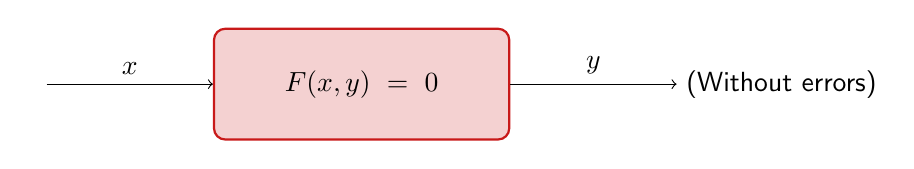
\begin{tikzpicture}
    \node [block] (func) {$F(x,y)=0$};
    \node [left of=func,node distance=4cm,anchor=east] (in) {};
    \node [right of=func,node distance=4cm,anchor=west] (out) {(Without errors)};
    \draw [->] (in) -- (func) node[midway,above] {$x$};
    \draw [->] (func) -- (out) node[midway,above] {$y$};
  \end{tikzpicture} \vskip1em \pause
  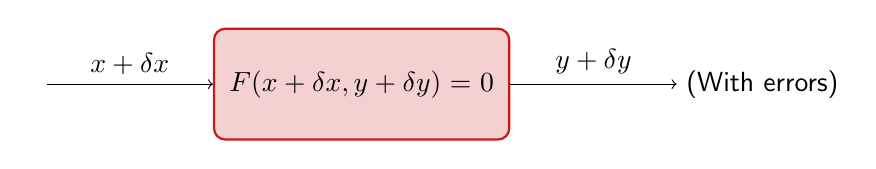
\begin{tikzpicture}
    \node [block] (func) {$F(x+\delta x,y+\delta y)=0$};
    \node [left of=func,node distance=4cm,anchor=east] (in) {};
    \node [right of=func,node distance=4cm,anchor=west] (out) {(With errors)};
    \draw [->] (in) -- (func) node[midway,above] {$x + \delta x$};
    \draw [->] (func) -- (out) node[midway,above] {$y + \delta y$};
  \end{tikzpicture}\pause
  \begin{columns}
  \column{0.5\textwidth}
  \[ y(x+\delta x) - y(x) \approx y'(x)\delta x \] 
  Propagated error on the basis of Taylor expansion
  \column{0.5\textwidth}
  \[ C = \operatorname*{max}_{\delta x} \left( \left | \frac{\delta y / y}{\delta x / x} \right| \right) \]
  Condition criterion, $C<10$ error development small
  \end{columns}
}

\begin{frame}[fragile]
  \frametitle{Badly (ill) conditioned problems: Example}
  Solve the following linear system in Matlab using double and single precision:\\
  $ A = 
      \left[\begin{aligned}
       1.2969 & & 0.8648 \\%[0.3em]
       0.2161 & & 0.1441
      \end{aligned}\right], \quad 
     x = \left[\begin{aligned}
       0.8642  \\%[0.3em]
       0.1440 
     \end{aligned}\right]
     \uncover<2->{, \quad 
     y = \left[\begin{aligned}
       2.0 \\%[0.3em]
       2.0 
     \end{aligned}\right]} $
\begin{columns}[T]
  \column{0.5\textwidth}
  \begin{block}<3->{Double precision}
    \begin{lstlisting}
>> clear;clc;format long e;
>> A = [[1.2969 0.8648]; [0.2161 0.1441]];
>> x = [0.8642; 0.1440];
>> y = A\x
y =
     2.000000002400302e+00
    -2.000000003599621e+00
    \end{lstlisting}
  \end{block}
  \pause 
  \column{0.5\textwidth}
    \begin{block}<4>{Single precision}
      \begin{lstlisting}
>> clear;clc;format long e;
>> A = single(
  [[1.2969 0.8648];
  [0.2161 0.1441]] );
>> x = single(
  [0.8642; 0.1440] );
>> y = A\x
y =
   1.3331791e+00
  -1.0000000e+00
    \end{lstlisting}
  \end{block}
\end{columns}
\end{frame}

\frame{ 
\frametitle{Badly (ill) conditioned problems: Example}
\begin{itemize}
  \colorize<1> \item Matlab already warned us about the bad condition number: \\
  \lstinline$Warning: Matrix is close to singular or badly scaled. Results may be inaccurate. RCOND =  1.148983e-08.$
  \colorize<2> \item The \lstinline$RCOND$ is the reciprocal condition number
%   \colorize<2> \item Using Gaussian elimination and fixing the numbers to 11 digits, we find:
%      \[ y = \left[\begin{aligned}
%        0.6662 \\%[0.3em]
%        -0.0002 
%      \end{aligned}\right] \]
    \colorize<3> \item A small error in $x$ results in a big error in $y$. This is called an ill conditioned problem.
  \end{itemize}
}

\section{(Un)stable methods}
\againframe<2>{contents_err}
\subsection*{Unstable methods}
\frame{
  \frametitle{(Un)stable methods}
  \begin{itemize}
    \item The condition criterion does not tell you anything about the quality of a numerical solution method!
    \item It is very well possible that a certain solution method is more sensitive for one problem than another
    \item If the method propagates the error, we call it an \emph{unstable method}. Let's look at an example.
  \end{itemize}
}

\frame{
  \frametitle{The Golden mean}
  \begin{itemize}
   \colorize<1> \item Let's evaluate the following recurrent relationship:
    \[ y_{n+1} = y_{n-1} - y_n \]
    \[ y_0 = 1, \quad y_1 = \frac{2}{1+\sqrt{5}} \]
    \colorize<2> \item You can prove (by substitution) that:
    \[ y_n = x^{-n}, \quad n=0,1,2,\ldots, \quad x = \frac{1 + \sqrt{5}}{2} \]
  \end{itemize}
}
% 
\begin{frame}[fragile]
  \frametitle{The Golden mean}
  \begin{columns}[T]
    \column{0.5\textwidth}
      \begin{block}{Recurrent version}
        \begin{lstlisting}
% initialise
y(1) = 1;
y(2) = 2 / (1 + sqrt(5));

% Perform recurrent approach
for n = 2:39
    y(n+1) = y(n-1)-y(n);
end
        \end{lstlisting}
      \end{block}
    \pause
    \column{0.5\textwidth}
      \begin{block}{Powerlaw version}
        \begin{lstlisting}
% initialise
x = (1 + sqrt(5))/2;
y2(1) = x^0; % n = 1

% Perform powerlaw apprach
for n = 0:39
    y2(n+1) = x^-n
end
        \end{lstlisting}
      \end{block}
  \end{columns}
\end{frame}
% 
\begin{frame}[fragile]
  \frametitle{The Golden mean}
    \begin{longtable}{c!{\vrule}cc}
    \hline
      $n$   & Recurrent & Powerlaw \\ \hline
      $1$   & $1.0000$ & $1.0000$ \\
      $1$   & $0.6180$ & $0.6180$ \\
      $2$   & $0.3820$ & $0.3820$ \\
      $3$   & $0.2361$ & $0.2361$ \\
      $\ldots$ & $\ldots$ & $\ldots$ \\
      $37$ & $3.080\cdot10^{-08}$ & $2.995\cdot10^{-08}$ \\
      $38$ & $1.714\cdot10^{-08}$ & $1.851\cdot10^{-08}$ \\
      $39$ & $1.366\cdot10^{-08}$ & $1.144\cdot10^{-08}$ \\
      $40$ & $3.485\cdot10^{-08}$ & $7.071\cdot10^{-08}$ \\ \hline
    \end{longtable} 
    \begin{itemize}
      \colorize<2> \item The recurrent approach enlarges errors from earlier calculations!
    \end{itemize}
\end{frame}

\frame{
 \frametitle{Example 1: Explanation}
 Recall example 1, where the errors blew up our computation of 0.1, whereas they did not for 2. Why did we see these results? \pause \\ \vskip2em
 \begin{itemize}
 \colorize<2> \item The number 0.1 is not exactly represented in binary
  \begin{itemize}
  \colorize<2> \item A tiny error can accumulate up to catastrophic proportions!
  \end{itemize}
  \colorize<3> \item The number 2 does have an exact binary representation
 \end{itemize}
}

\frame{
    \frametitle{Example 2 (large sine series)}
 
    The \lstinline$sin(1e40*pi)$ result gives poor results, because 1e40 has an error of \lstinline$eps$, about $1 \times 10^{-14}$. In Matlab, the number of $2*\pi$ cycles is still much larger than $10^{40}*10^{-14}$. Also, $\pi$ is not stored with enough digits.
 }
\frame{
 \frametitle{Example 3}
  Start your calculation program of choice (Excel, Matlab, ...) \vskip1em 
  
  \pause 
  Calculate the result of $y$:
  \[ y = e^{\pi} - \pi \onslide<3->{= 19.999099979\onslide<4->{\neq 20}}\]
  
  \uncover<5>{
  \vskip1em 
  \centering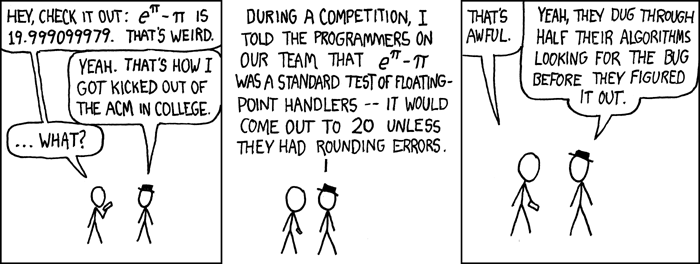
\includegraphics[width=0.8\textwidth]{e_to_the_pi_minus_pi}
  \begin{flushright}
  {\tiny
   Image: \href{http://www.xkcd.com/217/}{xkcd}}
  \end{flushright}
  }
}
 
\section{Symbolic math}
\againframe<2>{contents_err}
\subsection*{Symbolic math}
\frame{ 
  \frametitle{Symbolic math packages}
  \begin{definition}
   The use of computers to manipulate mathematical equations and expressions in symbolic form, as opposed to manipulating the numerical quantities represented by those symbols. 
  \end{definition}
  \vskip1em
  \begin{itemize}
   \item Symbolic integration or differentiation, substitution of one expression into another
   \item Simplification of an expression, change of subject etc.
   \item Packages and toolboxes:
  \end{itemize}
}

\frame{ 
  \frametitle{Symbolic math packages}

   \begin{description}[leftmargin=0.1cm]
    \item[\href{http://www.wolfram.com/mathematica/}{Mathematica}] 
      Well known software package, license available via \href{http://w3.tue.nl/nl/diensten/dienst_ict/services/services_wins/instelling_software/}{TU/e} \vskip0.5em
    \item[\href{http://www.maplesoft.com}{Maple}] 
 Well known, license available via \href{http://w3.tue.nl/nl/diensten/dienst_ict/services/services_wins/instelling_software/}{TU/e}\vskip0.5em
    \item[{\href{http://www.wolframalpha.com/}{Wolfram$|$Alpha}}] 
 Web-based interface by Mathematica developer. Less powerful in mathematical respect, but more accessible and has a broad application range (unit conversion, semantic commands).\vskip0.5em
    \item[\href{http://www.sagemath.org/}{Sage}] 
 Open-source alternative to Maple, Mathematica, Magma, and MATLAB.\vskip0.5em
    \item[\href{http://www.mathworks.nl/help/symbolic/index.html}{Matlab}] 
 Symbolic math toolbox
   \end{description}
}

\lstset{language=Matlab,
    escapeinside={(*@}{@*)}
}

\begin{frame}[fragile]
  \frametitle{Symbolic math: simplify}
  \[ f(x) = (x - 1) (x + 1) (x^2 + 1) + 1 \]
  \pause
  \begin{lstlisting}
>> syms x
>> f = (x - 1)*(x + 1)*(x^2 + 1) + 1
(*@ \pause @*) 
f =
 
(x^2 + 1)*(x - 1)*(x + 1) + 1
(*@ \pause @*) 
>> f2 = simplify(f)
(*@ \pause @*) 
f2 =
 
x^4
    \end{lstlisting}
\end{frame}

\begin{frame}[fragile]
  \frametitle{Symbolic math: integration and differentiation}
  \[ f(x) = \frac{1}{x^3+1} \]
  \pause
  \begin{lstlisting}
>> syms x
>> f = 1/(x^3+1);
>> my_f_int = int(f)
(*@ \pause @*) 
my_f_int = log(x + 1)/3 - log((x - 1/2)^2 + 3/4)/6 + (3^(1/2)*atan((2*3^(1/2)*(x - 1/2))/3))/3
(*@ \pause @*)
>> my_f_diff = diff(my_f_int)
 (*@ \pause @*)
my_f_diff = 1/(3*(x + 1)) + 2/(3*((4*(x - 1/2)^2)/3 + 1)) - (2*x - 1)/(6*((x - 1/2)^2 + 3/4))
(*@ \pause @*) 
>> simplify(my_f_diff)
(*@ \pause @*) 
ans = 1/(x^3 + 1)
    \end{lstlisting}
\end{frame}

\begin{frame}[fragile]
  \frametitle{Symbolic math: exercises}
  \begin{block}{Exercise 1}
  Simplify the following expression:
  \[ f(x) = \frac{2 \tan x }{(1 + \tan^2 x)} \uncover<2->{ = \sin 2x} \] \vskip-1em
  \pause
  \begin{lstlisting}
>> simplify(2*tan(x)/(1 + tan(x)^2))
  \end{lstlisting}
  \end{block}
  \pause
  \begin{block}{Exercise 2}
  Calculate the \emph{value} of $p$:
  \[  p = \int_0^{10} \frac{e^x - e^{-x}}{\sinh x}dx \] \vskip-1em
  \pause
  \begin{lstlisting}
>> f = ((exp(x)- exp(-x))/sinh(x));
>> p = int(f,0,10)
p = 20  
  \end{lstlisting}
  \end{block}
\end{frame}

\begin{frame}[fragile]
  \frametitle{Symbolic math: root finding }
  A root finding method searches for the values where a function reaches zero. We will cover the numerical methods later, here we show how to use root finding with symbolic math in Matlab.
  \begin{columns}[T]
   \column{0.5\textwidth}
   \begin{block}{Symbolic math function}
  \[ f(x) =   \frac{3}{x^2 + 3x} - 2 \]
  \pause
  \begin{lstlisting}
>> syms x
>> f = 3 / (x^2 + 3*x) - 2;
>> solve(f)
ans =
   15^(1/2)/2 - 3/2
 - 15^(1/2)/2 - 3/2
    \end{lstlisting}
   \end{block}
    \pause   
   \column{0.5\textwidth}
  \begin{block}{Function as a string}
\[ f(x) = x^2 - 4x + 2 \]
    \pause
    \begin{lstlisting}
>> solve('x^2 - 4*x + 2')
ans =
 2^(1/2) + 2
 2 - 2^(1/2)
    \end{lstlisting}
  \end{block}
  \end{columns}
\end{frame}

\begin{frame}[fragile]
  \frametitle{Symbolic math toolbox: variable precision arithmetic}
  Variable precision can be used to specify the number of significant digits.
      \begin{lstlisting}
>> p = vpa(1/3,16)
p = 0.3333333333333333
>> p = vpa(1/3,4)
p = 0.3333
>> a = vpa(0.1, 30)
a = 0.1
>> b = vpa(0.1, 5);
b = 0.1
>> a-b
 
ans = 0.0000000000000056843418860808014869689938467514
\end{lstlisting}
\end{frame}

 
\section{Summary}
\againframe<2>{contents_err}
\subsection*{Summary}
\begin{frame}
  \frametitle{Summary}
  \begin{itemize}
    \colorize<1> \item Numerical errors mar arise due to truncation, roundoff and break errors, which may seriously affect the accuracy of your solution
    \colorize<2> \item Errors may propagate and accumulate, leading to smaller accuracy
    \colorize<3> \item Ill-conditioned problems and unstable methods have to be identified so that proper measures can be taken
    \colorize<4> \item Symbolic math computations may be performed to solve certain equations algebraically, bypassing numerical errors, but this is not always possible.
  \end{itemize}

\end{frame}


% References
% http://ocw.mit.edu/courses/electrical-engineering-and-computer-science/6-00sc-introduction-to-computer-science-and-programming-spring-2011/unit-1/lecture-1-introduction-to-6.00/
% http://www.greenteapress.com/thinkpython/html/thinkpython002.html
% https://www.youtube.com/channel/UCLMQ21H2ad95faYG3yGCwYA
%http://stackoverflow.com/questions/4227145/in-matlab-are-variables-really-double-precision-by-default
%http://www.exploringbinary.com/why-0-point-1-does-not-exist-in-floating-point/



\title{Linear equations 1}
\subtitle{Linear algebra basics}
\lecture{Linear equations 1}{linear1}
\part{Systems of linear equations I - Introduction}
\section{Introduction}
\subsection*{General}
\begin{frame}[label=contentslin1]
  \frametitle{Today's outline}
  \mode<beamer>{
    \only<1>{\tableofcontents}
  }
  \only<2>{\tableofcontents[currentsection,currentsubsection]}
\end{frame}

\begin{frame}
  \frametitle{Overview}
  \begin{block}{Goals}
    \begin{itemize}
      \item Different ways of looking at a system of linear equations
      \item Determination of the inverse, determinant and the rank of a matrix
      \item The existence of a solution to a set of linear equations
  \end{itemize}
  \end{block}
\end{frame}
% 
\subsection*{Linear systems}

{\nologo
  \frame{\frametitle{Different views of linear systems}
    \begin{columns}
      \column{0.4\textwidth}
    \begin{itemize}
      \vskip-1ex
      \item Separate equations:\vspace{-1em}\begin{align*}
        x + y +  z &= 4 \\
        2x + y + 3z &= 7 \\
        3x + y + 6z &= 5
      \end{align*} \pause
      \item Matrix mapping $Mx=b$:\vspace{-1ex} \[ 
        \begin{bmatrix}
    1 & 1 & 1\\ 
    2 & 1 & 3\\ 
    3 & 1 & 6
        \end{bmatrix}
        \begin{bmatrix}
    x \\
    y \\
    z 
        \end{bmatrix} = 
        \begin{bmatrix}
    4 \\
    7 \\
    5 
        \end{bmatrix} 
        \]
        \pause
      \item Linear combination:\vspace{-1ex} \[ 
        x \begin{bmatrix}
    1\\
    2\\
    3
    \end{bmatrix} +
        y \begin{bmatrix}
    1\\
    1\\
    1
    \end{bmatrix} +
        z \begin{bmatrix}
    1\\
    3\\
    6
    \end{bmatrix} =
    \begin{bmatrix}
    4\\
    7\\
    5
        \end{bmatrix} 
      \]
      \end{itemize}
      \column{0.6\textwidth}
      \pause
      \centering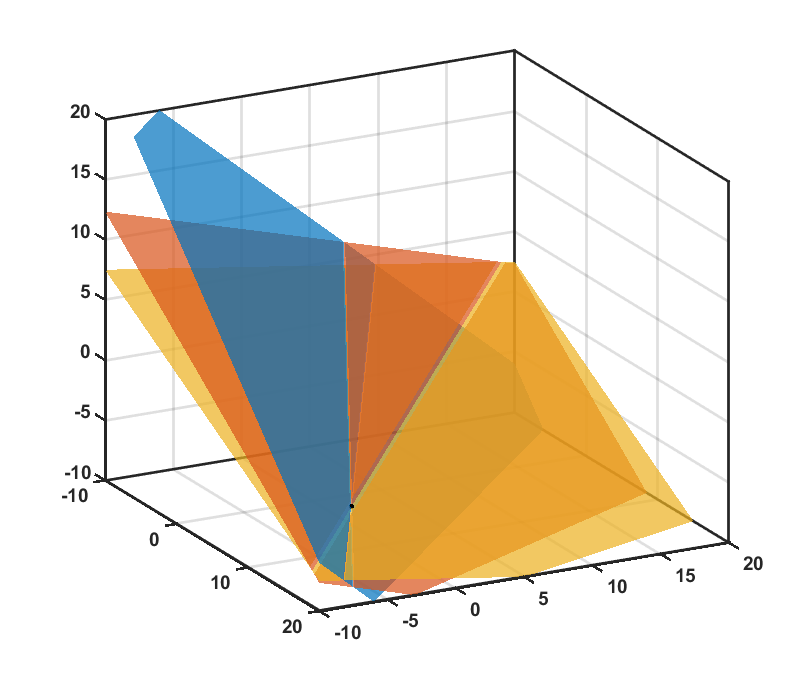
\includegraphics[width=\columnwidth]{planes_xing.png}
    \end{columns}
  }
}

\section{Matrix inversion}
\subsection*{Inverse}
\againframe<2>{contentslin1}

\frame{
  \frametitle{Inverse of a matrix}
  \begin{itemize}
    \item The inverse $M^{-1}$ is defined such that:
   \[ MM^{-1} = I \quad{} \text{and} \quad{} M^{-1}M=I\]
   \item Use the inverse to solve a set of linear equations:
   \begin{align*}
    M\vec{x} &= \vec{b} \\
    M^{-1}M\vec{x} &= M^{-1}\vec{b} \\
    I\vec{x} &= M^{-1}\vec{b} \\
    \vec{x} &= M^{-1}\vec{b}
   \end{align*}
  \end{itemize}
}
% 
\frame{\frametitle{How to calculate the inverse?}
  \begin{itemize}
    \item The inverse of an $N \times N$ matrix can be calculated using the co-factors of each element of the matrix:
    \[
      M^{-1} = \frac{1}{\det{M}}
      \begin{bmatrix}
      C_{00} &C_{01} &C_{02} \\
      C_{10} &C_{11} &C_{12} \\
      C_{20} &C_{21} &C_{22} \\
      \end{bmatrix}^T
    \]
    \item $\det{M}$ is the \emph{determinant} of matrix $M$.
    \item $C_{ij}$ is the \emph{co-factor} of the $ij^\text{th}$ element in $M$.
    \item $M^T$ indicates the transpose of a matrix $M$
  \end{itemize}
}

\begin{frame}[fragile]
\frametitle{Computing the co-factors}
  Consider the following example matrix:
  $ M =
    \begin{bmatrix}
      1 & 1 & 1\\ 
      2 & 1 & 3\\ 
      3 & 1 & 6
    \end{bmatrix} 
  $\\ \vskip1em \pause
  A co-factor (e.g. $C_{00}$) is the \tikzmarkin[txt=style green]{det1}determinant of the elements left over\tikzmarkend{det1} when you cover up the row and column of the \tikzmarkin[txt=style cyan]{cof}element in question\tikzmarkend{cof}, \tikzmarkin[txt=style orange]{pm1}multiplied by $\pm 1$\tikzmarkend{pm1}, depending on the position. \vskip1em
  \begin{columns}
    \column{0.25\textwidth}
      \begin{equation*}
      \left[\begin{array}{ccc}
	\tikzmarkin[mat=style cyan]{col 1} 1 \tikzmarkend{col 1} &  \times & \times \\
	\times  & \tikzmarkin[mat=style green]{col 2} 1 & 3 \\
	\times  &  1   &  6 \tikzmarkend{col 2}\\
	\end{array}\right]
      \end{equation*}\pause
    \column{0.25\textwidth}
      \begin{equation*}
      \left[\begin{array}{ccc}
	\tikzmarkin[mat2=style orange]{pm} + \tikzmarkend{pm} &  - & + \\
	- & + & - \\
	+ & - & +\\
	\end{array}\right]
      \end{equation*}\pause
      \column{0.5\textwidth}
      \[ \begin{split}
C_{00} &= \tikzmarkin[mat2=style orange]{pm3}+1\tikzmarkend{pm3}\ \cdot\ \det{\begin{array}{cc}\tikzmarkin[mat=style green]{det2} 1 & 3 \\ 1 & 6\tikzmarkend{det2}\end{array}} \\
&= 6 \times 1 - 3 \times 1 = 3
\end{split}
\]
  \end{columns}
\end{frame}

\frame{\frametitle{Computing the co-factors}
    Back to our example:
    \[
      M^{-1} = \begin{bmatrix}
      1 & 1 & 1 \\
      2 & 1 & 3 \\
      3 & 1 & 6 \\
    \end{bmatrix}^{-1} = 
      \frac{1}{\det{M}}
      \begin{bmatrix}
      3 & -3 & -1 \\
      -5&  3 &  2 \\
      2 & -1 & -1 \\
      \end{bmatrix}^T
    \]\pause
    \begin{itemize}
      \item The determinant is very important
      \item If $\det{M}=0$, the inverse does not exist (singular matrix)
      \begin{itemize}
        \item E.g. when a row contains only zeros, or when a row is a scalar multiple of another row.
      \end{itemize}
    \end{itemize}
}

\frame{\frametitle{Calculating the determinant}
    Compute the determinant by multiplication of each element on a row (or column) by its cofactor and adding the results:
    \[
    \det{\begin{bmatrix}
      \ \tikzmarkin[mat=style green]{horizontal}1 & 1 & 1 \tikzmarkend{horizontal}\\
      2 & 1 & 3 \\
      3 & 1 & 6 \ \end{bmatrix}} = +\det{\begin{bmatrix}1&3\\1&6\end{bmatrix}} - \det{\begin{bmatrix}2&3\\3&6\end{bmatrix}} + \det{\begin{bmatrix}2&1\\3&1\end{bmatrix}} = -1
    \]
    \pause
    \[
    \det{\begin{bmatrix}
      \ 1 & 1 & \tikzmarkin[mat=style green]{vertical}1 \\
      2 & 1 & 3 \\
      3 & 1 & 6\tikzmarkend{vertical}\ \end{bmatrix}} = +\det{\begin{bmatrix}2&1\\3&1\end{bmatrix}} - 3\det{\begin{bmatrix}1&1\\3&1\end{bmatrix}} + 6\det{\begin{bmatrix}1&1\\2&1\end{bmatrix}} = -1
    \]
}

\section{Solving a linear system}
\subsection*{Solving}
\againframe<2>{contentslin1}

\frame{\frametitle{Solving a linear system}
  \begin{itemize}
    \item Our example:
   \[ 
      \begin{bmatrix}
	1 & 1 & 1\\ 
	2 & 1 & 3\\ 
	3 & 1 & 6
      \end{bmatrix}
      \begin{bmatrix}
	x \\
	y \\
	z 
      \end{bmatrix} = 
      \begin{bmatrix}
	4 \\
	7 \\
	5 
      \end{bmatrix} 
      \]\pause
    \item The solution is:
    \[
    \begin{bmatrix}x \\ y \\ z\end{bmatrix} = M^{-1}b= \frac{1}{-1}
    \begin{bmatrix}
      3 & -5 & 2 \\
      -3&  3 & -1 \\
      -1 & 2 & -1 \\
    \end{bmatrix} \begin{bmatrix}4 \\ 7 \\ 5\end{bmatrix} = \frac{1}{-1}\begin{bmatrix}-13 \\ 4 \\ 5\end{bmatrix} = \begin{bmatrix}13 \\ -4 \\ -5\end{bmatrix}
    \]\pause
    \item The inverse exists, because $\det{M}=-1$.
  \end{itemize}
}

\begin{frame}[fragile]
  \frametitle{Solving a linear system in Python using the inverse}
  \begin{itemize}
    \item Set the scene by importing the right modules:
    \begin{lstlisting}
import numpy as np
import numpy.linalg as npla # scipy.linalg also works!
    \end{lstlisting}
    \item Create the matrix $A$ (explicit indication of datatype):
    \begin{lstlisting}
A = np.array([[1,1,1],[2,1,3],[3,1,6]],dtype=np.float64)
    \end{lstlisting}\pause
    \item Create solution vector (column vector):
    \begin{lstlisting}
b = np.array([[4.,7.,5.]]).T # Check b.shape!
    \end{lstlisting}\pause
    \item Get the matrix inverse; we use the linalg submodule
    \begin{lstlisting}
Ainv = npla.inv(A)
    \end{lstlisting}\pause
    \item Compute the solution:  \vspace{-1em}
    \begin{multicols}{2}
\begin{lstlisting}[linewidth=0.45\textwidth]
solution = Ainv.dot(b) # Alt: Ainv@b
print(f'The solution is:\n {solution}')
\end{lstlisting}      \break
\begin{lstlisting}[language=sh,style=output,linewidth=0.45\textwidth]
The solution is:
[[13.]
[-4.]
[-5.]]
\end{lstlisting}
\end{multicols}
  \end{itemize}
\end{frame}

\begin{frame}[fragile]
  \frametitle{Solving a linear system in Python: recommended approach}
  \begin{columns}
    \column{0.5\textwidth}
      NumPy approach
      \begin{lstlisting}
# solve_system_np.py
import numpy as np
import numpy.linalg as npla

A = np.array([[1.,1.,1.],[2.,1.,3.],[3.,1.,6.]])
b = np.array([[4.,7.,5.]]).T
x = npla.solve(A,b)
print(f'Solution using np linalg:\n {x}')
        \end{lstlisting}
        \begin{lstlisting}[style=output]
Solution using np linalg:
[[13.]
[-4.]
[-5.]]
        \end{lstlisting}
    \column{0.5\textwidth}
    SciPy approach
    \begin{lstlisting}
# solve_system_sp.py
import numpy as np
import scipy.linalg as spla

A = np.array([[1.,1.,1.],[2.,1.,3.],[3.,1.,6.]])
b = np.array([[4.,7.,5.]]).T
x = spla.solve(A,b)
print(f'Solution using sp linalg:\n {x}')      
      \end{lstlisting}
      \begin{lstlisting}[style=output]
Solution using sp linalg:
[[13.]
[-4.]
[-5.]]
    \end{lstlisting}
  \end{columns}
  Paraphrased from the NumPy manual:
  There is overlap in the functionality provided by the SciPy and NumPy submodules. SciPy contains functions not found in \lstinline$numpy.linalg$. Some functions that exist in both have augmented functionality in \lstinline$scipy.linalg$. Some functions in NumPy, however, have more flexible broadcasting options.
\end{frame}

\begin{frame}<beamer:0|handout:1>[fragile]
  \frametitle{Exercise: performance of inverse computation}
  Create a script that generates matrices with random elements of various sizes $N\times N$ (e.g. values of $N\in\left\{10,20,50,100,200,\ldots,5000,10000\right\}$). Compute the inverse of each matrix, and use \lstinline$tic$ and \lstinline$toc$ to see the computing time for each inversion. Plot the time as a function of the matrix size $N$.
  \vskip2em
  \begin{hints}
  Hints:
  \begin{itemize}
      \item Create an array that contains the sizes of the systems $n$
      \item Loop over the array elements to:
      \begin{itemize}
          \item Create a random matrix of size $n\times n$
          \item Perform the matrix inversion
          \item Record the time required
      \end{itemize}
      \item Plot the time required for inversion vs size of the system on a double-log scale
  \end{itemize}
  \end{hints}
\end{frame}

{\nologo
\begin{frame}<handout:0|beamer:1->[fragile]
  \frametitle{Exercise: performance of inverse computation}
  Create a script that generates matrices with random elements of various sizes $N\times N$ (e.g. values of $N\in\left\{10,20,50,100,200,\ldots,5000,10000\right\}$). Compute the inverse of each matrix, and use \lstinline$tic$ and \lstinline$toc$ to see the computing time for each inversion. Plot the time as a function of the matrix size $N$. \pause
    \begin{lstlisting}
import numpy as np
import scipy.linalg as spla
from time import time
import matplotlib.pyplot as plt

matrix_sizes = list(range(10,100,10)) + list(range(100,1100,100)) + list(range(2000,6000,1000)) + [10000]

for size in matrix_sizes: (*@ \pause @*)
    print(f'Currently processing matrix size: {size}x{size}')
    random_matrix = np.random.random((size,size)) (*@ \pause @*)
    start_time = time()
    spla.inv(random_matrix)
    total_time = time() - start_time
    time_to_inv.append(total_time)
    (*@ \pause @*)
plt.loglog(matrix_sizes,time_to_inv, 'r-x')
plt.xlabel('Matrix size')
plt.ylabel('Time to invert [s]')
plt.show()
  \end{lstlisting}
\end{frame}
}

\begin{frame}[fragile]
  \frametitle{Exercise: sample results}
  Each computer produces slightly different results because of background tasks, different matrices, etc. This is especially noticable for small systems.
  \begin{center}
  \begin{tikzpicture}
    \begin{loglogaxis}[
      xlabel={$N$},
      ylabel={Time [s]},
%       grid = major,
      width=0.6\textwidth, height=5.5cm]
     \addplot[graph,draw=tuered,thick,mark = x] table [y index={1}] {data/tictocINV.dat};
     \addplot [black,very thick] table {
	900 0.065
	11000 64.87
      } coordinate [pos=0.15] (A) % save two points on the regression line for drawing the slope triangle
        coordinate [pos=0.85] (B);
	\draw[thick] (A) -| (B)  % draw the opposite and adjacent sides of the triangle
        node [pos=0.25, anchor=north] {1} % label the horizontal line
        node [pos=0.75,anchor=west] {3};
     \end{loglogaxis}
  \end{tikzpicture}
  \end{center}
  \vskip-1em
  \tikzmarkin[txt=style white]{complexity}The time increases by 3 orders of magnitude, for every magnitude in $N$. The \emph{computational complexity} of matrix inversion scales with $\mathcal{O}(N^3)$!\tikzmarkend{complexity}
\end{frame}

% \begin{frame}[fragile]
%   \frametitle{Solving a linear system in Excel using the inverse}\vspace{-1em}
%   \[
%    Ax=b \qquad \begin{bmatrix}1&1&1\\2&1&3\\3&1&6\end{bmatrix}\begin{bmatrix}x_1\\x_2\\x_3\end{bmatrix}=\begin{bmatrix}4\\7\\5\end{bmatrix}
%   \]\vspace{-1em}
%   \begin{itemize}
%     \item Create matrix \ \tikzmarkin[mat=style green]{A}$A$\tikzmarkend{A} \ in $3\times 3$ cells
%     \item Create right hand side vector \ \tikzmarkin[mat=style cyan]{b}$b$\tikzmarkend{b} \ in 3 vertical cells\pause
%     \item Compute the inverse \ \tikzmarkin[mat=style orange]{I}$I$\tikzmarkend{I} \ :
%     \begin{itemize}
%       \item Select an empty area of $3 \times 3$ cells
%       \item Type \lstinline$=MINVERSE($
%       \tikzmarkin[txt=style green]{A2}\lstinline$B2:D4$\tikzmarkend{A2}
%       \lstinline$)$ (In Dutch Excel: \lstinline$INVERSEMAT$)
%       \item Close with Ctrl+Shift+Enter
%     \end{itemize}\pause
%     \item Solution:
%     \begin{itemize}
%       \item Select 3 vertical cells
%       \item Type \lstinline$=MMULT($
%       % First part, contains the inverse
%       \tikzmarkin[txt=style orange]{I2}\lstinline$H2:J4$\tikzmarkend{I2}
%       % Semicolon
%       \lstinline$;$
%       % Second part, contains the RHS
%       \tikzmarkin[txt=style cyan]{b2}\lstinline$B6:B8$\tikzmarkend{b2}
%       % Finish the command
%       \lstinline$)$ (In Dutch Excel: \lstinline$PRODUCTMAT$. The semicolon may be a comma.)
%       \item Close with Ctrl+Shift+Enter
%     \end{itemize}    
%   \end{itemize}
% \end{frame}


\section{Towards larger systems}
\subsection*{Matrix tricks}
\againframe<2>{contentslin1}

\begin{frame}[fragile]
  \frametitle{Towards larger systems}
  \tikz{\node[emphblock,text width=\textwidth] {Computation of determinants and inverses of large matrices in this way is too difficult (slow), so we need other methods to solve large linear systems!};}
\end{frame}

\begin{frame}[fragile]
  \frametitle{Towards larger systems}
  \begin{itemize}
    \item Determinant of upper triangular matrix:
    \[
    \det{M_\text{tri}} = \prod_{i=1}^n a_{ii} \qquad M=\begin{bmatrix}
5 & 3 & 2 \\ 
0 & 9 & 1 \\
0 & 0 & 1
\end{bmatrix} \Rightarrow \det{M} = 5 \times 9 \times 1 = 45
    \]
  \item Matrix multiplication:
  \[
  \det{AM}=\det{A}\times\det{M}
  \]
  \item When $A$ is an identity matrix ($\det{A}=1$):
  \[
   \det{AM}=\det{A}\times\det{M} = 1\times\det{M}
  \]
  \item With rules like this, we can use row-operations so that we can compute the determinant more cheaply.
  \end{itemize}
\end{frame}

\subsection*{Rank}
\begin{frame}[fragile]
  \frametitle{Solutions of linear systems}
 Rank of a matrix: the number of linearly independent columns (columns that can not be expressed as a linear combination of the other columns) of a matrix.
 \vskip1em
 \begin{columns}
  \column{0.5\textwidth}
  \[
   M = \begin{bmatrix}
        5 & 3 & 2 \\
        0 & 9 & 1 \\
        0 & 0 & 1
       \end{bmatrix}
  \]
  \begin{itemize}
   \item 3 independent columns
   \item In Matlab:
   \begin{lstlisting}
import numpy.linalg as npla
npla.matrix_rank(A)
   \end{lstlisting}
  \end{itemize}
  \column{0.5\textwidth}
    \[
   M = \left[\begin{array}{cccc}
        \tikzmarkin[mat=style green]{c1}1 & \tikzmarkin[mat=style yellow]{c2}2 & \tikzmarkin[mat=style cyan]{c3}1 & \tikzmarkin[mat=style orange]{c4}0 \\
        0 & 0 & 1 & 1 \\
        0\tikzmarkend{c1} & 0\tikzmarkend{c2} & 0\tikzmarkend{c3} & 0\tikzmarkend{c4}
       \end{array}\right]
  \]
  \begin{itemize}
   \item \tikzmarkin[txt=style yellow]{c22}col 2\tikzmarkend{c22} $= 2 \times$ \tikzmarkin[txt=style green]{c12}col 1\tikzmarkend{c12}
   \item \tikzmarkin[txt=style orange]{c42}col 4\tikzmarkend{c42} $=$ \tikzmarkin[txt=style cyan]{c32}col 3\tikzmarkend{c32} $-$ \tikzmarkin[txt=style green]{c13}col 1\tikzmarkend{c13}
   \item 2 independent columns: rank = 2
  \end{itemize}
 \end{columns}
\end{frame}

\begin{frame}[fragile]
  \frametitle{Solutions of linear systems}
  The solution of a system of linear equations may or may not exist, and it may or may not be unique. Existence of solutions can be determined by comparing the rank of the Matrix $M$ with the rank of the augmented matrix $M_a$:
  \begin{columns}
    \column{0.5\textwidth}
    \begin{lstlisting}
import numpy as np
import numpy.linalg as npla

M = np.array([[5.,3.,2.],[0.,9.,1.],[0.,0.,1.]])
print(f'{M} has rank: {npla.matrix_rank(M)}\n')

b = np.array([[3.],[4.],[5.]])
M_aug = np.hstack((M,b))
print(f'{M_aug} has rank: {npla.matrix_rank(M_aug)}')
    \end{lstlisting}
    \column{0.5\textwidth}
    \begin{lstlisting}[style=output]
[[5. 3. 2.]
 [0. 9. 1.]
 [0. 0. 1.]] has rank: 3

[[5. 3. 2. 3.]
 [0. 9. 1. 4.]
 [0. 0. 1. 5.]] has rank: 3
    \end{lstlisting}
  \end{columns}
  Our system: $Mx = b$
  \[ 
    M = \begin{bmatrix}
    M_{11} & M_{12} & M_{13}\\ 
    M_{21} & M_{22} & M_{23}\\ 
    M_{31} & M_{32} & M_{33}
    \end{bmatrix} \text{,} b=\begin{bmatrix}b_1\\b_2\\b_3  \end{bmatrix} \Rightarrow 
    M_a =     \begin{bmatrix}
    M_{11} & M_{12} & M_{13} & b_1\\ 
    M_{21} & M_{22} & M_{23} & b_2\\ 
    M_{31} & M_{32} & M_{33} & b_3
    \end{bmatrix}
  \]
\end{frame}

\begin{frame}
 \frametitle{Existence of solutions for linear systems}
  For a matrix $M$ of size $n \times n$, and augmented matrix $M_a$:
 \begin{columns}
  \column{0.5\textwidth}
 \begin{itemize}
   \item $\text{Rank}(M) = n$:\\ Unique solution
 \end{itemize}
  \column{0.5\textwidth}
   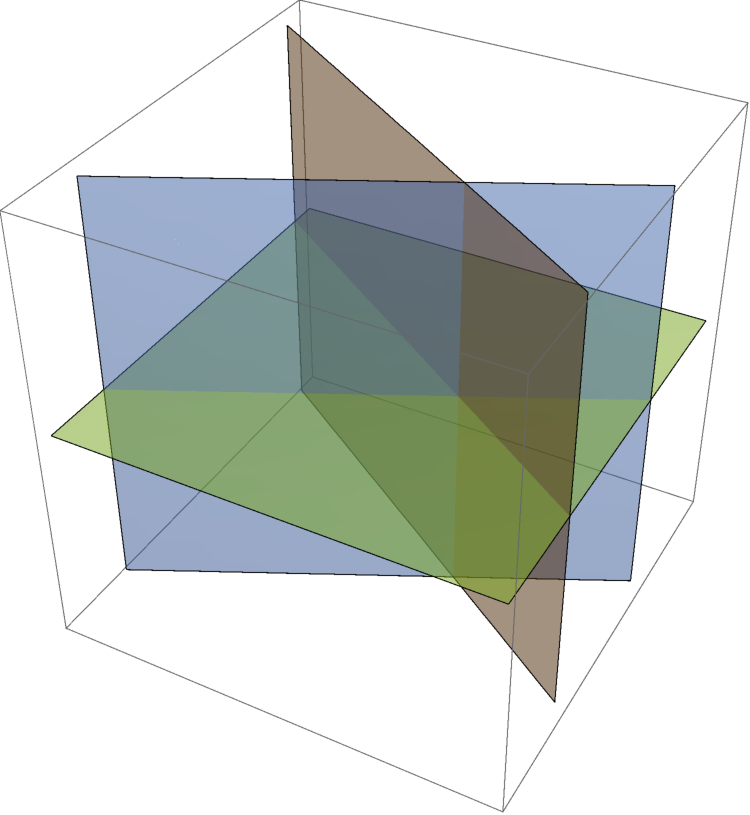
\includegraphics[width=0.3\columnwidth]{Rank_1-solution}
 \end{columns}
 \pause
  \begin{columns}
  \column{0.5\textwidth}
 \begin{itemize}
   \item $\text{Rank}(M) = \text{Rank}(M_a) < n$:\\ Infinite number of solutions
 \end{itemize}
  \column{0.5\textwidth}
   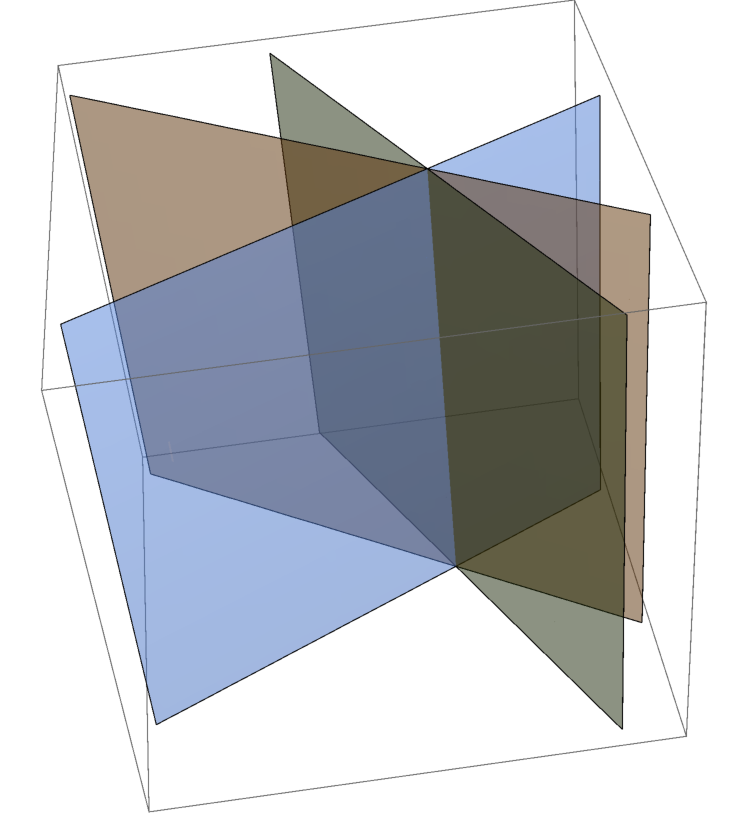
\includegraphics[width=0.3\columnwidth]{Rank_Inf-solutions}
 \end{columns}
 \pause
  \begin{columns}
  \column{0.5\textwidth}
 \begin{itemize}
   \item $\text{Rank}(M) < n$, $\text{Rank}(M) < \text{Rank}(M_a)$:\\ No solutions
 \end{itemize}
  \column{0.5\textwidth}
   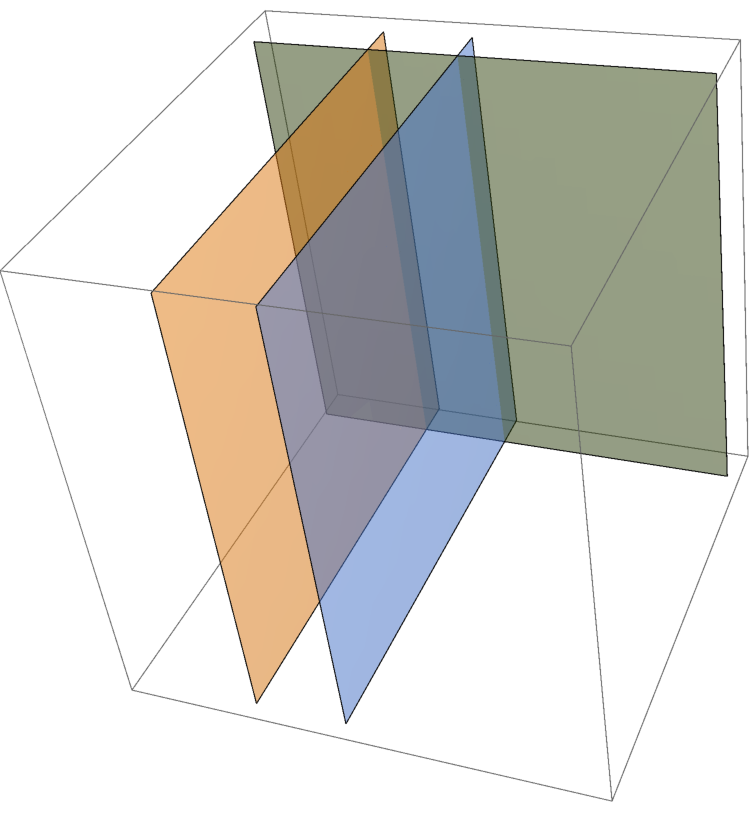
\includegraphics[width=0.3\columnwidth]{Rank_No-solutions1} \ \ 
   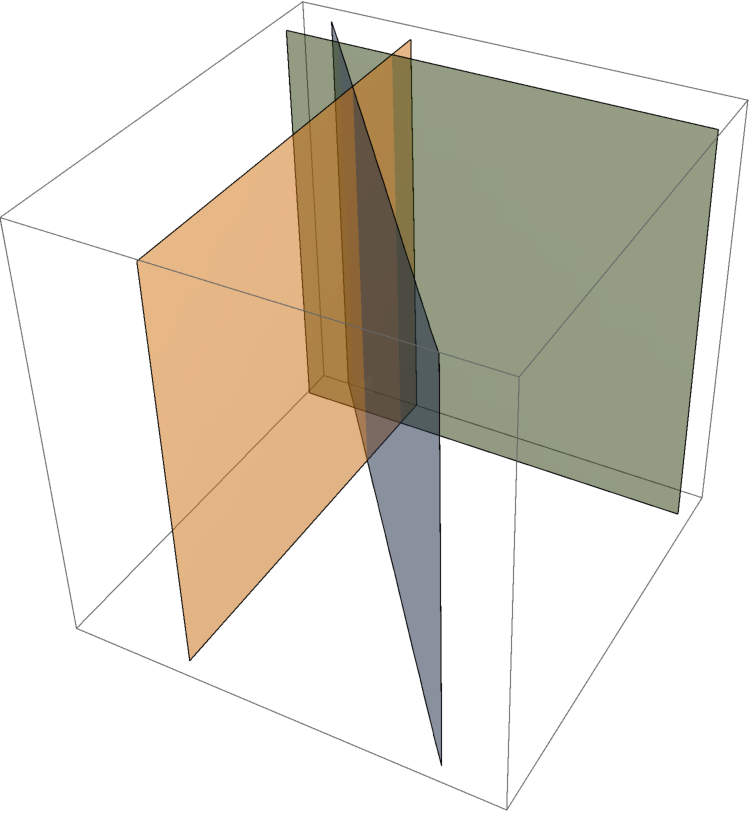
\includegraphics[width=0.3\columnwidth]{Rank_No-solutions2}
 \end{columns}
\end{frame}
 
\begin{frame}[fragile]
  \frametitle{Two examples}
  \[
    M=
    \begin{bmatrix}
      1 & 1 & 2\\
      0 & 3 & 1\\
      0 & 0 & 2
    \end{bmatrix}\quad
    b=
    \begin{bmatrix}
      17\\11\\4
    \end{bmatrix}
    \Rightarrow
    M_a=
    \begin{bmatrix}
      1 & 1 & 2 & 17\\
      0 & 3 & 1 & 11\\
      0 & 0 & 2 & 4
    \end{bmatrix}
  \]
  $\rank(M)=3=n \Rightarrow $ Unique solution \pause \\ \vfill
    \[
    M=
    \begin{bmatrix}
      1 & 1 & 2\\
      0 & 3 & 1\\
      0 & 0 & 0
    \end{bmatrix}\quad
    b=
    \begin{bmatrix}
      17\\11\\0
    \end{bmatrix}
    \Rightarrow
    M_a=
    \begin{bmatrix}
      1 & 1 & 2 & 17\\
      0 & 3 & 1 & 11\\
      0 & 0 & 0 & 0
    \end{bmatrix}
  \]
  $\rank(M)=\rank(M_a)=2<n \Rightarrow $ Infinite number of solutions
\end{frame} 

\section{Summary}
\subsection*{Summary}
\againframe<2>{contentslin1}

\begin{frame}[fragile]
  \frametitle{Summary}
  \begin{itemize}
    \item Linear equations can be written as matrices
    \item Using the inverse, the solution can be determined
    \begin{itemize}
      \item Inverse via cofactors
      \item Inverse and solution in Matlab
      \item Inverse and solution in Excel
    \end{itemize}
    \item Introduced the concept of computational complexity: matrix inversion scales with $N^3$
    \item A solution depends on the rank of a matrix
  \end{itemize}
\end{frame}

\title{Linear equations 2}
\subtitle{Direct methods}
\lecture{Linear equations 2}{linear2}
\part{Systems of linear equations I - Direct methods}
\section{Introduction}
\subsection*{General}
\begin{frame}[label=contents_lin2]
  \frametitle{Today's outline}
  \mode<beamer>{
    \only<1>{\tableofcontents}
  }
  \only<2>{\tableofcontents[currentsection,currentsubsection]}
\end{frame}

\begin{frame}
  \frametitle{Overview}
  \begin{block}{Goals}
    Today we are going to write a program, which can solve a set of linear equations
    \begin{itemize}
      \item The first method is called Gaussian elimination
      \item We will encounter some problems with Gaussian elimination
      \item Then LU decomposition will be introduced
  \end{itemize}
  \end{block}
\end{frame}

\section{Gauss elimination}
\subsection*{Row operations}
\againframe<2>{contents_lin2}
\frame{
  \frametitle{Define the linear system}
   Consider the system: 
   \[
      Ax = b
   \]
   \vfill
   In general:
    \[ 
    \begin{bmatrix}
A_{00} & A_{01} & A_{02}\\ 
A_{10} & A_{11} & A_{12}\\ 
A_{20} & A_{21} & A_{22}
\end{bmatrix}\begin{bmatrix}
x_0\\x_1\\x_2  
\end{bmatrix}=\begin{bmatrix}b_0\\b_1\\b_2  \end{bmatrix} 
\]
  \vfill
Desired solution:
    \[ 
    \begin{bmatrix}
1 & 0 & 0\\ 
0 & 1 & 0\\ 
0 & 0 & 1
\end{bmatrix}\begin{bmatrix}
x_0\\x_1\\x_2  
\end{bmatrix}=\begin{bmatrix}b'_0\\b'_1\\b'_2\end{bmatrix} 
\]
}

\begin{frame}[fragile]
  \frametitle{Using row operations}
  \begin{itemize}
    \item Use row operations to simplify the system. Eliminate element $A_{10}$ by subtracting $A_{10}/A_{00} = d_{10}$ times row 1 from row 2.
    \item In this case, Row 1 is the pivot row, and $A_{00}$ is the pivot element.
  \end{itemize}
  \tikz{\node (m1) {
    $
    \left[\begin{array}{ccc|c}
      A_{00} & A_{01} & A_{02} & b_0\\ 
      \tikzmarkin[txt=style yellow]{a21a} A_{10} & A_{11} & A_{12} & b_1\tikzmarkend{a21a}\\ 
      A_{20} & A_{21} & A_{22} & b_2
    \end{array}\right]
  $};
  \node[right=2cm of m1,](m2){
  $
    \left[\begin{array}{ccc|c}
      A_{00} & A_{01} & A_{02} & b_0\\ 
      \tikzmarkin[txt=style yellow] {a21b} 0      & A'_{11} & A'_{12} & b'_1\tikzmarkend{a21b}\\ 
      A_{20} & A_{21} & A_{22} & b_2
    \end{array}\right]
  $};
  \draw[->,thick] (m1.east) --  (m2.west);
  }
\end{frame}

\begin{frame}[fragile]
  \frametitle{Using row operations}
  Eliminate element $A_{10}$ using $d_{10}=A_{10}/A_{00}$.
  \vfill
    \tikz{\node (m1) {
    $
    \left[\begin{array}{ccc|c}
      A_{00} & A_{01} & A_{02} & b_0\\ 
      \tikzmarkin[txt=style yellow] {a211}A_{10} & A_{11} & A_{12} & b_1\tikzmarkend{a211}\\ 
      A_{20} & A_{21} & A_{22} & b_2
    \end{array}\right]
  $};
  \node[right=2cm of m1,](m2){
  $
    \left[\begin{array}{ccc|c}
      A_{00} & A_{01} & A_{02} & b_0\\ 
      \tikzmarkin[txt=style yellow] {a212} 0      & A'_{11} & A'_{12} & b'_1\tikzmarkend{a212}\\ 
      A_{20} & A_{21} & A_{22} & b_2
    \end{array}\right]
  $};
  \draw[->,thick] (m1.east) --  (m2.west);
  }
  \vfill\pause
  \begin{columns}
  \column{0.4\textwidth}
  \begin{itemize}
    \item $d_{10}\rightarrow A_{10}/A_{00}$
    \item $A_{10}\rightarrow A_{10}-A_{00}d_{10}$
    \item $A_{11}\rightarrow A_{11}-A_{01}d_{10}$
    \item $A_{12}\rightarrow A_{12}-A_{02}d_{10}$
    \item $b_1   \rightarrow b_1   -b_0   d_{10}$
  \end{itemize}
  \pause
  \column{0.6\textwidth}
   \begin{lstlisting}
d10 = A[1,0] / A[0,0]

A[1,0] = A[1,0] - A[0,0] * d10
A[1,1] = A[1,1] - A[0,1] * d10
A[1,2] = A[1,2] - A[0,2] * d10

b[1] = b[1] - b[0] * d10
   \end{lstlisting}
  \end{columns}
\end{frame}

\begin{frame}[fragile]
  \frametitle{Using row operations}
  Eliminate element $A_{20}$ using $d_{20}=A_{20}/A_{00}$.
  \vfill
    \tikz{\node (m1) {
    $
    \left[\begin{array}{ccc|c}
      A_{00} & A_{01} & A_{02} & b_0\\ 
      0 & A'_{11} & A'_{12} & b'_1\\ 
      \tikzmarkin[txt=style yellow] {a311}A_{20} & A_{21} & A_{22} & b_2\tikzmarkend{a311}
    \end{array}\right]
  $};
  \node[right=2cm of m1,](m2){
  $
    \left[\begin{array}{ccc|c}
      A_{00} & A_{01} & A_{02} & b_0\\ 
      0      & A'_{11} & A'_{12} & b'_1\\ 
      \tikzmarkin[txt=style yellow] {a312}0 & A'_{21} & A'_{22} & b'_2\tikzmarkend{a312}
    \end{array}\right]
  $};
  \draw[->,thick] (m1.east) --  (m2.west);
  }
  \vfill\pause
  \begin{columns}
  \column{0.4\textwidth}
  \begin{itemize}
    \item $d_{20}\rightarrow A_{20}/A_{00}$
    \item $A_{20}\rightarrow A_{20}-A_{00}d_{20}$
    \item $A_{21}\rightarrow A_{21}-A_{01}d_{20}$
    \item $A_{22}\rightarrow A_{22}-A_{02}d_{20}$
    \item $b_2   \rightarrow b_2   -b_0   d_{20}$
  \end{itemize}
  \column{0.6\textwidth}
  \begin{lstlisting}
d20 = A[2, 0] / A[0, 0]

A[2, 0] = A[2, 0] - A[0, 0] * d20
A[2, 1] = A[2, 1] - A[0, 1] * d20
A[2, 2] = A[2, 2] - A[0, 2] * d20
b[2] = b[2] - b[0] * d20
  \end{lstlisting}
  \end{columns}
\end{frame}

\begin{frame}[fragile]
  \frametitle{Using row operations}
  Eliminate element $A'_{21}$ using $d_{21}=A'_{21}/A'_{11}$. Note that now the second row has become the pivot row.
  \vfill
    \tikz{\node (m1) {
    $
    \left[\begin{array}{ccc|c}
      A_{00} & A_{01} & A_{02} & b_0\\ 
      0 & A'_{11} & A'_{12} & b'_1\\ 
      \tikzmarkin[txt=style yellow] {a311b} 0 & A'_{21} & A'_{22} & b'_2\tikzmarkend{a311b}
    \end{array}\right]
  $};
  \node[right=2cm of m1,](m2){
  $
    \left[\begin{array}{ccc|c}
      A_{00} & A_{01} & A_{02} & b_0\\ 
      0      & A'_{11} & A'_{12} & b'_1\\ 
      \tikzmarkin[txt=style yellow] {a312b}0 & 0 & A''_{22} & b''_2\tikzmarkend{a312b}
    \end{array}\right]
  $};
  \draw[->,thick] (m1.east) --  (m2.west);
  }
  \vfill\pause
  \begin{columns}
  \column{0.4\textwidth}
  \begin{itemize}
    \item $d_{21}\rightarrow A_{21}/A'_{11}$
    \item $A_{21}\rightarrow A_{21}-A'_{11}d_{21}$
    \item $A_{22}\rightarrow A_{22}-A'_{12}d_{21}$
    \item $b_2   \rightarrow b_2   -b'_2   d_{21}$
  \end{itemize}
  \column{0.6\textwidth}
   \begin{lstlisting}
d21 = A[2, 1] / A[1, 1]
A[2, 1] = A[2, 1] - A[1, 1] * d21
A[2, 2] = A[2, 2] - A[1, 2] * d21
b[2] = b[2] - b[1] * d21
   \end{lstlisting}
  \end{columns}
  \pause
  \vfill
  The matrix is now a triangular matrix --- the solution can be obtained by back-substitution.
\end{frame}

\subsection*{Backsubstitution}
\begin{frame}[fragile]
  \frametitle{Backsubstitution}
  The system now reads:
  \[
    \begin{bmatrix}
      A_{00} & A_{01} & A_{02}\\ 
      0      & A'_{11} & A'_{12}\\ 
      0 & 0 & A''_{22}
    \end{bmatrix}
    \begin{bmatrix}x_0\\x_1\\x_2\end{bmatrix} = 
    \begin{bmatrix}b_0\\b'_1\\b''_2\end{bmatrix}
  \]
  \pause
  Start at the last row $N$, and work upward until row 1.
  \begin{columns}
  \column{0.4\textwidth}
    \begin{align*}
     x_2 &= b''_2/A''_{22}\\
     x_1 &= (b'_1 - A'_{12}x_2)/A'_{11}\\
     x_0 &= (b_0 - A_{01}x_1 - A_{02}x_2)/A_{00}
    \end{align*}
    \pause
  \column{0.6\textwidth}
    \begin{lstlisting}
x = np.empty_like(b)
x[2] = b[2] / A[2,2]
x[1] = (b[1] - A[1,2] * x[2]) / A[1,1]
x[0] = (b[0] - A[0,1] * x[1] - A[0,2] * x[2]) / A[0,0]
    \end{lstlisting}
\end{columns}
In general:
\[
 x_N = \frac{b_N}{A_{NN}} \qquad x_i = \frac{b_i - \sum_{j=i+1}^{N}A_{ij}x_j}{A_{ii}}
\]
\end{frame}

\begin{frame}[fragile]
  \frametitle{Writing the program}
  \begin{itemize}
   \item Create a function that provides the framework: take matrix $A$ and vector $b$ as an input, and return the solution $x$ as output:
  \begin{lstlisting}[language=Python]
def gaussian_eliminate(A, b):
    pass  # Your implementation here
  \end{lstlisting}
  \item We will use \emph{for-loops} instead of typing out each command line.
  \item Useful Python (with NumPy) shortcuts:
  \begin{itemize}
  \item \lstinline[language=Python]$A[0, :]$   = $[A_{00}, A_{01}, A_{02}]$
  \item \lstinline[language=Python]$A[:, 1]$   = $[A_{01}, A_{11}, A_{21}]$
  \item \lstinline[language=Python]$A[0, 1:]$ = $[A_{01}, A_{02}]$
  \end{itemize}
  \item A row operation could look like:
  \begin{lstlisting}[language=Python]
A[i, :] = A[i, :] - d * A[0, :]   
  \end{lstlisting}
  \end{itemize}
\end{frame}


\begin{frame}[fragile]
  \frametitle{The program: elimination step}
  An initial draft could look like:
  \begin{lstlisting}
def gaussian_eliminate_draft(A,b):
    """Perform elimination to obtain an upper triangular matrix"""
    A = np.array(A,dtype=np.float64)
    b = np.array(b,dtype=np.float64)

    assert A.shape[0] == A.shape[1], "Coefficient matrix should be square"

    N = len(b)
    for col in range(N-1):                # Select pivot
        for row in range(col+1,N):        # Loop over rows below pivot
            d = A[row,col] / A[col,col]   # Choose elimination factor
            for element in range(row,N):  # Elements from diagonal to right
                A[row,element] = A[row,element] - d * A[col,element]
            b[row] = b[row] - d * b[col]

    return A,b
  \end{lstlisting}
\end{frame}

\begin{frame}[fragile]
  \frametitle{The program: elimination step}
  Employing some of the row operations to create \lstinline|gaussian_eliminate_v1|:
  \begin{columns}[T]
    \column{0.6\textwidth}
    \begin{lstlisting}
for element in range(row,N):
    A[row,element] = A[row,element] - d * A[col,element]
        \end{lstlisting}    
    \column{0.4\textwidth}
    \begin{lstlisting}
A[row,:] = A[row,:] - d * A[col,:]
        \end{lstlisting}
  \end{columns}
  \pause
  \begin{lstlisting}
def gaussian_eliminate_v1(A,b):
    A = np.array(A,dtype=np.float64)
    b = np.array(b,dtype=np.float64)

    assert A.shape[0] == A.shape[1], "Coefficient matrix should be square"

    N = len(b)
    for col in range(N-1):
        for row in range(col+1,N):
            d = A[row,col] / A[col,col]
            A[row,:] = A[row,:] - d * A[col,:]
            b[row] = b[row] - d * b[col]

    return A,b
  \end{lstlisting}
\end{frame}

\begin{frame}[fragile]
  \frametitle{Testing}
  Let's try to eliminate our linear system! If you create/downloaded our file \lstinline|gaussjordan.py|, you can access the functions by importing them. The file should be stored where your own code/notebook is:
  \begin{lstlisting}
from gaussjordan import gaussian_eliminate_draft,gaussian_eliminate_v1
import numpy as np

A = np.array([[1, 1, 1], [2, 1, 3], [3, 1, 6]]) 
b = np.array([4, 7, 5]) 

Aprime,bprime = gaussian_eliminate_draft(A,b)
print(Aprime)
print(bprime)
  \end{lstlisting}
\end{frame}

\begin{frame}[fragile]
  \frametitle{The program: Backsubstitution}
  Now we have elimination working, let's create a back substitution algorithm too. Recall:
  \[
    x_N = \frac{b_N}{A_{NN}} \qquad x_i = \frac{b_i - \sum_{j=i+1}^{N}A_{ij}x_j}{A_{ii}}
 \]
 \begin{columns}[T]
  \column{0.4\textwidth}
  \begin{lstlisting}[basicstyle=\tiny\ttfamily]
def backsubstitution_draft(A, b):
    """Back substitutes an upper triangular matrix to find x in Ax=b"""
    x = np.copy(b)
    N = len(b)

    for row in range(N-1, -1, -1):
        for i in range(row+1, N):
            x[row] = x[row] - A[row, i] * x[i]
        x[row] = x[row] / A[row, row]  
    
    return x
      \end{lstlisting}\pause
  \column{0.6\textwidth}
  \begin{lstlisting}[basicstyle=\tiny\ttfamily]
def backsubstitution_v1(A,b):
    """Back substitutes an upper triangular matrix to find x in Ax=b"""
    x = np.empty_like(b)
    N = len(b)
    
    for row in range(N)[::-1]:
        x[row] = (b[row] - np.sum(A[row,row+1:] * x[row+1:])) / A[row,row]

    return x
      \end{lstlisting}
 \end{columns}
\end{frame}

% \begin{frame}[fragile]
%   \frametitle{The program: Backsubstitution}
%   \begin{lstlisting}
% def backsubstitution_v1(A,b):
%     """Back substitutes an upper triangular matrix to find x in Ax=b"""
%     x = np.empty_like(b)
%     N = len(b)
    
%     for row in range(N)[::-1]:
%         x[row] = (b[row] - np.sum(A[row,row+1:] * x[row+1:])) / A[row,row]

%     return x
%   \end{lstlisting}
%   \[
%      x_N = \frac{b_N}{A_{NN}} \qquad x_i = \frac{b_i - \sum_{j=i+1}^{N}A_{ij}x_j}{A_{ii}}
%   \]
% \end{frame}

\begin{frame}[fragile]
  \frametitle{A full Gauss Elimination solver}
  \begin{itemize}
    \item The functions we just built are distributed via Canvas too
    \item Use \lstinline$help GaussianEliminate$ to find out how it works
    \item Solve the following system of equations:
    \[
    \begin{bmatrix}
      9 & 9 & 5 & 2\\ 
      6 & 7 & 1 & 3\\ 
      6 & 4 & 3 & 5\\
      2 & 6 & 2 & 1
    \end{bmatrix}
    \begin{bmatrix}x_1\\x_2\\x_3\\x_4\end{bmatrix} = 
    \begin{bmatrix}7\\4\\10\\1\end{bmatrix}
  \]
  \item Compare your solution with \lstinline$np.linalg.solve(A,b)$
  \end{itemize}
\end{frame}

\section{Partial Pivoting}
\subsection*{Pivoting}
\againframe<2>{contents_lin2}

\begin{frame}[fragile]
  \frametitle{Partial pivoting}
  \begin{itemize}
    \item Now try to run the algorithm with the following system:
    \[
    \begin{bmatrix}
      0 & 2 & 1\\ 
      3 & 2 & 1 \\ 
      1 & 1 & 1
    \end{bmatrix}
    \begin{bmatrix}x_1\\x_2\\x_3\end{bmatrix} = 
    \begin{bmatrix}4\\3\\10\end{bmatrix}
  \]
  \pause
  \item It does not work! Division by zero, due to $A_{11}=0$.
  \item Solution: Swap rows to move largest element to the diagonal.
  \end{itemize}
\end{frame}

\begin{frame}[fragile]
  \frametitle{Partial pivoting: implementing row swaps}
  \begin{itemize}[<+->]
    \item Find maximum element row below pivot in current column
    \begin{lstlisting}[numbers=none]
index = np.argmax(np.abs(A[col:, col])) + col 
    \end{lstlisting}
    \item Store current row
    \begin{lstlisting}[numbers=none]
temp = A[column,:]
    \end{lstlisting}
    \item Swap pivot row and desired row in \lstinline$A$
    \begin{lstlisting}[numbers=none]
A[column,:] = A[index,:]
A[index,:] = temp
      \end{lstlisting}
    \item Do the same for \lstinline$b$ --- store and swap
    \begin{lstlisting}[numbers=none]
temp = b[column]
b[column] = b[index]
b[index] = temp
      \end{lstlisting}
  \end{itemize}
\end{frame}

\begin{frame}[fragile]
  \frametitle{Adding the partial pivoting rules}
  \begin{lstlisting}[language=Python]
def gaussian_eliminate_partial_pivot(A,b):
    A = np.array(A,dtype=np.float64)
    b = np.array(b,dtype=np.float64)

    assert A.shape[0] == A.shape[1], "Coefficient matrix should be square"

    N = len(b)
    for col in range(N-1):
        index = np.argmax(np.abs(A[col:, col])) + col
        temp = A[col,:]
        A[col,:] = A[index,:]
        A[index,:] = temp

        temp = b[col]
        b[col] = b[index]
        b[index] = temp
        for row in range(col+1,N):
            d = A[row,col] / A[col,col]
            A[row,:] = A[row,:] - d * A[col,:]
            b[row] = b[row] - d * b[col]

    return A,b
  \end{lstlisting}
\end{frame}

\begin{frame}[fragile]
  \frametitle{Improve the program by using re-usable functions}
  \begin{lstlisting}[language=Python]
def swap_rows(mat,i1,i2):
    """Swap two rows in a matrix/vector"""
    temp = mat[i1,...].copy()
    mat[i1,...] = mat[i2,...]
    mat[i2,...] = temp
  \end{lstlisting}
  \begin{lstlisting}[language=Python]
def gaussian_eliminate_v2(A,b):
    A = np.array(A,dtype=np.float64)
    b = np.array(b,dtype=np.float64)

    assert A.shape[0] == A.shape[1], "Coefficient matrix should be square"

    N = len(b)
    for col in range(N-1):
        index = np.argmax(np.abs(A[col:, col])) + col
        swap_rows(A,col,index)
        swap_rows(b,col,index)
        for row in range(col+1,N):
            d = A[row,col] / A[col,col]
            A[row,:] = A[row,:] - d * A[col,:]
            b[row] = b[row] - d * b[col]

    return A,b
  \end{lstlisting}
\end{frame}

\begin{frame}[fragile]
  \frametitle{Alternatives to this program}
  \begin{itemize}
    \item Python can compute the solution to Ax=b with \lstinline|scipy.linalg.solve| or \lstinline|numpy.linalg.solve| solvers (more efficient)
    \item Too many loops. Loops make Python slow.
    \item There are fundamental problems with Gaussian elimination\pause
    \begin{itemize}
      \item You can add a counter to the algorithm to see how many subtraction and multiplication operations it performs for a given size of matrix A.
      \item The number of operations to perform Gaussian elimination is $\mathcal{O}(2N^3)$ (where $N$ is the number of equations) 
      \item Exercise: verify this for our script \pause
      \item LU decomposition takes $\mathcal{O}(2N^3/3)$ flops, 3 times less!
      \item Forward and backward substitution each take $\mathcal{O}(N^2)$
flops (both cases) 
    \end{itemize}
  \end{itemize}
\end{frame}

\section{LU decomposition}
\subsection*{LU}
\againframe<2>{contents_lin2}

\begin{frame}[fragile]
  \frametitle{LU Decomposition}
  Suppose we want to solve the previous set of equations, but with several right hand sides:
    \[ 
    \begin{bmatrix}
A_{11} & A_{12} & A_{13}\\ 
A_{21} & A_{22} & A_{23}\\ 
A_{31} & A_{32} & A_{33}
\end{bmatrix}
\begin{bmatrix}
\vdots & \vdots & \vdots \\
x_1 & x_2 & x_3 \\
\vdots & \vdots & \vdots
\end{bmatrix} = 
\begin{bmatrix}
\vdots & \vdots & \vdots \\
b_1 & b_2 & b_3 \\
\vdots & \vdots & \vdots
\end{bmatrix}
\]\pause
Factor the matrix A into two matrices, L and U, such that $A=LU$:
\[ 
    \begin{bmatrix}
A_{11} & A_{12} & A_{13}\\ 
A_{21} & A_{22} & A_{23}\\ 
A_{31} & A_{32} & A_{33}
\end{bmatrix} = 
\begin{bmatrix}
1 & 0 & 0 \\
\times & 1 & 0 \\
\times & \times & 1
\end{bmatrix}
\begin{bmatrix}
\times & \times & \times \\
0 & \times & \times \\
0 & 0 & \times
\end{bmatrix}
\]
Now we can solve for each right hand side, using only a forward
followed by a backward substitution!
\end{frame}

\begin{frame}[fragile]
  \frametitle{Substitutions}
  \begin{itemize}
    \item Define a lower and upper matrix $L$ and $U$ so that $A = LU$
    \item Therefore $LUx = b$
    \item Define a new vector $y = Ux$ so that $Ly = b$
    \item Solve for $y$, use $L$ and forward substitution
    \item Then we have $y$, solve for $x$, use $Ux = y$
    \item Solve for $x$, use $U$ and backward substitution
    \item But how to get L and U?
  \end{itemize}
\end{frame}

\begin{frame}[fragile]
  \frametitle{Decomposing the matrix (1)}
  When we eliminate the element $A_{21}$ we can keep multiplying by a matrix that undoes this row operations, so that the product remains equal to $A$.
\[ 
\begin{bmatrix}
A_{11} & A_{12} & A_{13}\\ 
A_{21} & A_{22} & A_{23}\\ 
A_{31} & A_{32} & A_{33}
\end{bmatrix} = 
\begin{bmatrix}
1 & 0 & 0 \\
d_{21}& 1 & 0 \\
0 & 0 & 1
\end{bmatrix}
\begin{bmatrix}
A_{11} & A_{12} & A_{13}\\ 
0 & A_{22}-d_{21}A_{12} & A_{23}-d_{21}A_{13}\\ 
A_{31} & A_{32} & A_{33}
\end{bmatrix}
\]
\end{frame}

\begin{frame}[fragile]
  \frametitle{Decomposing the matrix (2)}
  When we eliminate the element $A_{31}$ we can keep multiplying by a matrix that undoes this row operations, so that the product remains equal to $A$.
\[ 
A = 
\begin{bmatrix}
1 & 0 & 0 \\
d_{21}& 1 & 0 \\
d_{31} & 0 & 1
\end{bmatrix}
\begin{bmatrix}
A_{11} & A_{12} & A_{13}\\ 
0 & A'_{22}=A_{22}-d_{21}A_{12} & A'_{23} = A_{23}-d_{21}A_{13}\\ 
0 & A'_{32} = A_{32}-d_{31}A_{12} & A'_{33} = A_{33}-d_{31}A_{21}
\end{bmatrix}
\]
\end{frame}

\begin{frame}[fragile]
  \frametitle{Decomposing the matrix (3)}
  When we eliminate the element $A_{32}$ we can keep multiplying by a matrix that undoes this row operations, so that the product remains equal to $A$.
\[ 
\begin{bmatrix}
A_{11} & A_{12} & A_{13}\\ 
A_{21} & A_{22} & A_{23}\\ 
A_{31} & A_{32} & A_{33}
\end{bmatrix} = 
\begin{bmatrix}
1 & 0 & 0 \\
d_{21}& 1 & 0 \\
d_{31} & d_{32} & 1
\end{bmatrix}
\begin{bmatrix}
A_{11} & A_{12} & A_{13}\\ 
0 & A'_{22} & A'_{23} \\ 
0 & 0  & A''_{33} = A'_{33}-d_{32}A'_{23}
\end{bmatrix}
\]\pause
We now have a lower matrix $L$ and an upper matrix $U$. This finishes the LU decomposition! 
\end{frame}

\subsection*{Pivoting in LU decomposition}
{\nologo
\begin{frame}[fragile]
\frametitle{Pivoting during decomposition}
Suppose we have arrived at the situation below, where $A'_{32}>A'_{22}$:
\vfill
\[ 
\begin{bmatrix}
A_{11} & A_{12} & A_{13}\\ 
A_{21} & A_{22} & A_{23}\\ 
A_{31} & A_{32} & A_{33}
\end{bmatrix} = 
\begin{bmatrix}
1 & 0 & 0 \\
d_{21}& 1 & 0 \\
d_{31} & 0 & 1
\end{bmatrix}
\begin{bmatrix}
A_{11} & A_{12} & A_{13}\\ 
0 & \tikzmarkin[mat=style tueturq]{n1} A'_{22} & A'_{23} \\ 
0 & A'_{32}\tikzmarkend{n1} & A'_{33} 
\end{bmatrix}
\]
\vfill 
\pause
Exchange rows 2 and 3 to get the largest value on the main diagonal. Use a permutation matrix to store the swapped rows:
\vfill
\pause
\[ 
\begin{bmatrix}
\tikzmarkin[txt=style tueturq]{n2} 1 & 0 & 0 \\
0& 0 & 1 \\
0 & 1 & 0 \tikzmarkend{n2}
\end{bmatrix}
\begin{bmatrix}
A_{11} & A_{12} & A_{13}\\ 
A_{21} & A_{22} & A_{23}\\ 
A_{31} & A_{32} & A_{33}
\end{bmatrix} = 
\begin{bmatrix}
1 & 0 & 0 \\
\tikzmarkin[txt=style tueorange]{n3} d_{31}& 0 & 1 \tikzmarkend{n3}\\
\tikzmarkin[txt=style tueorange]{n4} d_{21} & 1 & 0 \tikzmarkend{n4}
\end{bmatrix}
\begin{bmatrix}
A_{11} & A_{12} & A_{13}\\ 
\tikzmarkin[txt=style tueorange]{n5}0 & A'_{32} & A'_{33} \tikzmarkend{n5}\\ 
\tikzmarkin[txt=style tueorange]{n6}0 & A'_{22} & A'_{23} \tikzmarkend{n6} 
\end{bmatrix}
\]
\pause
Multiplying with a permutation matrix will swap the rows of a matrix. The permutation matrix is just an identity matrix, whose rows
have been interchanged.
\end{frame}
}
% 
% \begin{frame}[fragile]
% \frametitle{Pivoting during decomposition}
% Multiplying with a permutation matrix will swap the rows of a matrix. The permutation matrix is just an identity matrix, whose rows
% have been interchanged.
% \vfill
% \[ 
% \begin{bmatrix}
% 1 & 0 & 0 \\
% 0& 0 & 1 \\
% 0 & 1 & 0
% \end{bmatrix}
% \begin{bmatrix}
% A_{11} & A_{12} & A_{13}\\ 
% A_{21} & A_{22} & A_{23}\\ 
% A_{31} & A_{32} & A_{33}
% \end{bmatrix} = 
% \begin{bmatrix}
% 1 & 0 & 0 \\
% d_{31}& 0 & 1 \\
% d_{21} & 1 & 0
% \end{bmatrix}
% \begin{bmatrix}
% A_{11} & A_{12} & A_{13}\\ 
% 0 & A'_{32} & A'_{33} \\ 
% 0 & A'_{22} & A'_{23} 
% \end{bmatrix}
% \]
% \end{frame}

\begin{frame}[fragile]
  \frametitle{Recipe for LU decomposition}
   When decomposing matrix $A$ into $A=LU$, it may be beneficial to swap rows to get the largest values on the diagonal of $U$ (pivoting). A permutation matrix $P$ is used to store row swapping such that:
   \[
    PA = LU
   \]
  \begin{itemize}
    \item Write down a permutation matrix and the linear system
    \item Promote the largest value in the column diagonal
    \item Eliminate all elements below diagonal
    \item Move on to the next column and move largest elements to diagonal
    \item Eliminate elements below diagonal
    \item Repeat 5 and 6
    \item Write down L,U and P
  \end{itemize}
\end{frame}

\subsection*{LU decomposition with pivoting-example}
\begin{frame}[fragile]
  \frametitle{LU decomposition example (1)}
  Write down a permutation matrix, which starts as the identity matrix, and the linear system:
  \begin{align*}
    PA &= LU \\
    \begin{bmatrix}
      1 & 0 & 0\\
      0 & 1 & 0\\
      0 & 0 & 1
    \end{bmatrix} 
    \begin{bmatrix}
      0 & 1 & 1\\
      2 & 1 & 1\\
      1 & 2 & 0
      \end{bmatrix}&= 
      \begin{bmatrix}
      1 & 0 & 0\\
      0 & 1 & 0\\
      0 & 0 & 1
      \end{bmatrix}
      \begin{bmatrix}
      0 & 1 & 1\\
      2 & 1 & 1\\
      1 & 2 & 0
      \end{bmatrix}
  \end{align*}
  \pause
  Promote the largest value into the diagonal of column 1 --- swap row 1 and 2:
    \[
      \begin{bmatrix}
	\tikzmarkin[txt=style yellow]{am1} 0 & 1 & 0\\
	1 & 0 & 0 \tikzmarkend{am1}\\
	0 & 0 & 1
      \end{bmatrix} 
      \begin{bmatrix}
	0 & 1 & 1\\
	2 & 1 & 1\\
	1 & 2 & 0
      \end{bmatrix}= 
      \begin{bmatrix}
	1 & 0 & 0\\
	0 & 1 & 0\\
	0 & 0 & 1
      \end{bmatrix}
      \begin{bmatrix}
	\tikzmarkin[txt=style yellow]{am2}2 & 1 & 0\\
	0 & 1 & 1 \tikzmarkend{am2}\\
	1 & 2 & 0
      \end{bmatrix}
    \]
\end{frame}
% 
\begin{frame}[fragile]
  \frametitle{LU decomposition example (2)}
  Eliminate all \tikzmarkin[txt=style tueorange]{lu1}elements below the diagonal\tikzmarkend{lu1} --- row 2 already contains a zero in column 1, row 3 = row 3 - 0.5 row 1. Record the \tikzmarkin[txt=style tuesteel]{lu2}multiplier 0.5\tikzmarkend{lu2} in $L$:
  \[
    \begin{bmatrix}
      0 & 1 & 0\\
      1 & 0 & 0\\
      0 & 0 & 1
    \end{bmatrix} 
    \begin{bmatrix}
      0 & 1 & 1\\
      2 & 1 & 1\\
      1 & 2 & 0
      \end{bmatrix}= 
      \begin{bmatrix}
      1 & 0 & 0\\
      0 & 1 & 0\\
      \tikzmarkin[txt=style tuesteel]{lu3}0.5\tikzmarkend{lu3} & 0 & 1
      \end{bmatrix}
      \begin{bmatrix}
      2 & 1 & 1\\
      \tikzmarkin[txt=style tueorange]{lu4}0 & 1 & 1\\
      0\tikzmarkend{lu4} & 1.5 & -0.5
      \end{bmatrix}
  \]
  \pause
  Elimination of column 1 is done. Now step to the next column, and move the largest value below/on the diagonal to the diagonal (~\tikzmarkin[txt=style yellow]{lu8}swap rows 2 and 3\tikzmarkend{lu8}~). Adjust $P$ and the \tikzmarkin[txt=style tueturq]{lu9}lower triangle of $L$\tikzmarkend{lu9} accordingly:
  \[
    \begin{bmatrix}
      0 & 1 & 0\\
      \tikzmarkin[txt=style yellow]{lu5} 0 & 0 & 1 \\
      1 & 0 & 0\tikzmarkend{lu5}
    \end{bmatrix} 
    \begin{bmatrix}
      0 & 1 & 1\\
      2 & 1 & 0\\
      1 & 2 & 0
      \end{bmatrix}= 
      \begin{bmatrix}
      1 & 0 & 0\\
      \tikzmarkin[draw=none,txt=style tueturq]{lu6}(0.25,-0.15)0.5 & 1 & 0\\
      \tikzmarkin[draw=none,txt=style tueturq]{lu10}0\tikzmarkend{lu6} & 0\tikzmarkend{lu10} & 1
      \end{bmatrix}
      \begin{bmatrix}
      2 & 1 & 1\\
      \tikzmarkin[txt=style yellow]{lu7}(0.4,-0.15) 0 & 1.5 & -0.5 \\
      0 & 1 & 1\tikzmarkend{lu7}
      \end{bmatrix}
  \]
\end{frame}

\begin{frame}[fragile]
  \frametitle{LU decomposition example (3)}
    Eliminate \tikzmarkin[txt=style tueorange]{f3}all elements below the diagonal\tikzmarkend{f3} ---\\
    row 3 = row 3 - $\frac{2}{3}$row 2. Record the multiplier \tikzmarkin[txt=style tueturq]{f1}$\frac{2}{3}$\tikzmarkend{f1} in $L$:
  \[
    \begin{bmatrix}
      0 & 1 & 0\\
      0 & 0 & 1 \\
      1 & 0 & 0
    \end{bmatrix} 
    \begin{bmatrix}
      0 & 1 & 1\\
      2 & 1 & 0\\
      1 & 2 & 0
      \end{bmatrix}= 
      \begin{bmatrix}
      1 & 0 & 0\\
      0.5 & 1 & 0\\
      0 & \tikzmarkin[txt=style tueturq]{f2}\frac{2}{3}\tikzmarkend{f2} & 1
      \end{bmatrix}
      \begin{bmatrix}
      2 & 1 & 1\\
      0 & 1.5 & -0.5 \\
      0 & \tikzmarkin[txt=style tueorange]{f4}0\tikzmarkend{f4} & \frac{4}{3}\\
      \end{bmatrix}
  \]
  \pause
  We have obtained the matrices from $PA=LU$:
  \[
    P = \begin{bmatrix}
      0 & 1 & 0\\
      0 & 0 & 1 \\
      1 & 0 & 0
    \end{bmatrix} \quad
    L=\begin{bmatrix}
      1 & 0 & 0\\
      0.5 & 1 & 0\\
      0 & \frac{2}{3} & 1
      \end{bmatrix} \quad
      U = \begin{bmatrix}
      2 & 1 & 1\\
      0 & 1.5 & -0.5 \\
      0 & 0 & \frac{4}{3}\\
      \end{bmatrix}
  \]
  Proceed with solving for $x$.
\end{frame}

\begin{frame}[fragile]
  \frametitle{Substitutions}
  \vskip-2em
  \begin{align*}
    Ax = b \quad  &\Rightarrow \quad PAx=Pb\equiv d\\
    PA = LU \quad&\Rightarrow \quad LUx = d
  \end{align*}
%   \vskip-1ex
  \begin{itemize}
    \item Define a new vector $y=Ux$
    \begin{itemize}
      \item $Ly=b \quad\Rightarrow\quad Ly = d$
      \item Solve for $y$, forward substitution:
      \begin{align*}
	y_0 &= \frac{d_0}{L_{00}} \\
	y_i &= \frac{d_i - \sum_{j=0}^{i}L_{ij}y_j}{L_{ii}}
      \end{align*}
    \end{itemize}
    \item Then solve $Ux=y$:
    \begin{itemize}
      \item Solve for $x$, backward substitution:
      \begin{align*}
	x_N &= \frac{y_N}{U_{NN}} \\
	x_i &= \frac{y_i - \sum_{j=i+1}^{N}U_{ij}x_j}{U_{ii}}
      \end{align*}
    \end{itemize}      
  \end{itemize}  
\end{frame}

\subsection*{Using LU in Python}
\begin{frame}[fragile]
  \frametitle{How to use the solver in Python}
  \begin{lstlisting}[language=Python]
import numpy as np
from scipy.linalg import lu
from gaussjordan import backsubstitution_v1 as backwardSub
from gaussjordan import forwardsubstitution as forwardSub

# Example usage
A = np.random.rand(5, 5)  # Get random matrix
P, L, U = lu(A)           # Get L, U and P
b = np.random.rand(5)     # Random b vector
d = P @ b                 # Permute b vector
y = forwardSub(L, d)      # Can also do y=L\d
x = backwardSub(U, y)     # Can also do x=U\y
rnorm = np.linalg.norm(A @ x - b)  # Residual
  \end{lstlisting}
  \pause
  \begin{itemize}
     \item Use this as a basis to create a function that takes $A$ and $b$, and returns $x$.
     \item Use the function to check the performance for various matrix sizes and inspect the performance.
  \end{itemize}

\end{frame}
\section{Summary}
\subsection*{Summary}
\againframe<2>{contents_lin2}

\begin{frame}[fragile]
  \frametitle{Summary}
  \begin{itemize}
    \item This lecture covered direct methods using elimination techniques.
    \item Gaussian elimination can be slow ($\mathcal{O}(N^3)$)
    \item Back substitution is often faster ($\mathcal{O}(N^2)$)
    \item LU decomposition means that we don't have to do Gaussian elimination every time (saves time and effort), but the matrix has to stay the same.
    \item Python's libraries have built in routines for solving linear equations and LU decomposition.
    \item Advanced techniques such as (preconditioned) conjugate gradient or biconjugate gradient solvers are also available.
    \item Next part covers iterative approaches
\end{itemize}
\end{frame}


\title{Linear equations 3}
\subtitle{Iterative methods}
\lecture{Linear equations 3}{linear3}
\part{Systems of linear equations I - Iterative methods}
\section{Introduction}
\subsection*{General}
\begin{frame}[label=contents_lin3]
  \frametitle{Today's outline}
  \mode<beamer>{
    \only<1>{\tableofcontents}
  }
  \only<2>{\tableofcontents[currentsection,currentsubsection]}
\end{frame}

\section{Sparse matrices}
\subsection*{Sparse matrices}

\begin{frame}[fragile]
  \frametitle{Sparse matrices}
  \begin{itemize}
    \item In many engineering cases, we deal with sparse matrices (as opposed to dense matrices)
    \item A matrix is sparse when it mostly consists of zeros
    \item Linear systems where equations depend on a limited number of variables (e.g. spatial discretization)
    \item Storing zeros is not very efficient:
    \begin{lstlisting}[language=Python]
import numpy as np
from scipy.sparse import csr_matrix

A = np.eye(10000)
print(A.nbytes)

S = csr_matrix(A)
print(S.data.nbytes)      
    \end{lstlisting}
    \item Can you think of a way to achieve this?
    \item Sparse matrix formats: Yale, CRS, CCS
\end{itemize}
\end{frame}

\begin{frame}[fragile]
  \frametitle{Sparse matrix storage format}
  \begin{columns}
  \column{0.6\textwidth}
  \begin{itemize}
    \item Example: Yale storage format, storing 3 vectors:
    \begin{itemize}
      \item \lstinline$A = [5 8 3 6]$
      \item \lstinline$IA = [0 1 2 3 4]$
      \item \lstinline$JA = [0 1 2 1]$
    \end{itemize}
  \end{itemize}
  \column{0.4\textwidth}
  \[
   A = 
   \begin{bmatrix}
    5 & 0 & 0 & 0\\
    0 & 8 & 0 & 0\\
    0 & 0 & 3 & 0\\
    0 & 6 & 0 & 0
    \end{bmatrix}
  \]
  \end{columns}
  \begin{itemize}
    \item \lstinline$A$ stores the non-zero values
    \item \lstinline$IA$ stores the index in A of the first non-zero in row i
    \item \lstinline$JA$ stores the column index
    \item Note: zero-based indices are used here!
\end{itemize}
\end{frame}

\begin{frame}[fragile]
  \frametitle{Sparse matrix layout examples}
  \begin{center}
   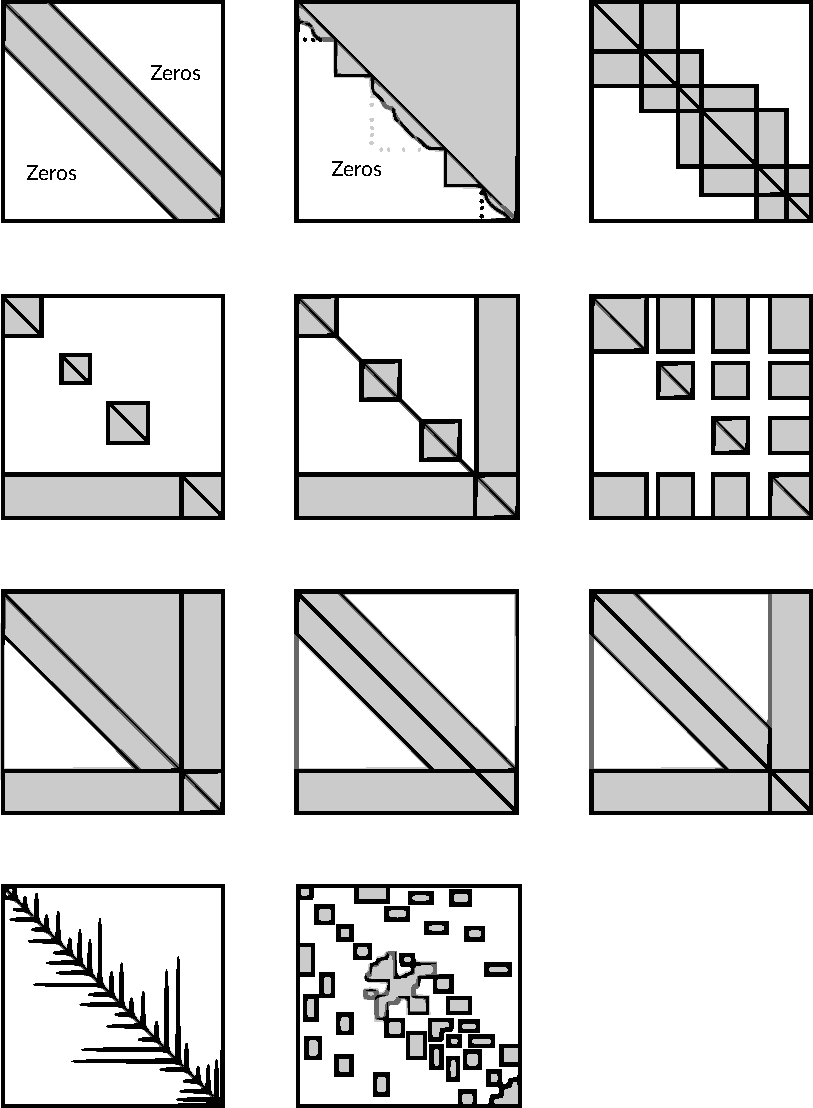
\includegraphics[height=0.8\textheight]{sparse-overview}
  \end{center}
\end{frame}

\section{Laplace's equation}
\subsection*{Laplace's equation}
\againframe<2>{contents_lin3}
\begin{frame}[fragile]
  \frametitle{Laplace's equation}
  \begin{columns}
  \column{0.7\textwidth}
  \begin{align*}
    \frac{\partial T}{\partial t} &= \alpha \nabla^2 T \\
    T &= \text{Temperature} \\
    \alpha &= \text{Thermal diffusivity}
  \end{align*}
  \pause
  \begin{center}
      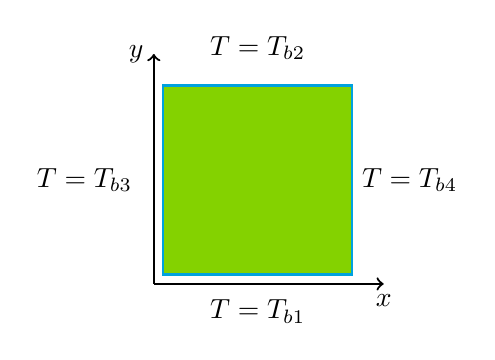
\begin{tikzpicture}[scale=0.4]
      \draw[black,thick,->] (-0.3,-0.3)-- node[at end,anchor=north]{$x$}(7,-0.3);
      \draw[black,thick,->] (-0.3,-0.3)-- node[at end,anchor=east]{$y$} (-0.3,7);
      \draw[thick,draw=tuelblue,fill=tuegreen] (0,0) rectangle +(6,6);
      \node[anchor=west] at (6,3) {$T=T_{b4}$};
      \node[above,anchor=south] at (3,6.5) {$T=T_{b2}$};
      \node[below,anchor=north] at (3,-0.5  ) {$T=T_{b1}$};
      \node[left of=3pt] at (0,3) {$T=T_{b3}$};
%       \node at (0.3,0.3) (A) {};
%       \node at (0.3,5.7) (B) {};
%       \node at (5.7,5.7) (C) {};
%       \node at (5.7,0.3) (D) {};
%       \draw[thick,tuered] (A) -- node[midway,anchor=east] {$T=T_{b3}$} (B);
%       \draw[thick,tuegreen] (B) -- node[midway,anchor=south] {$T=T_{b2}$} (C);
%       \draw[thick,tueorange] (C) -- node[midway,anchor=east] {$T=T_{b4}$} (D);
%       \draw[thick,tuepurple] (D) -- node[midway,anchor=south] {$T=T_{b1}$} (A);
      \end{tikzpicture}
    \end{center}
    \pause
  \column{0.3\textwidth}
  In steady state:
  \[
   \nabla^2 T = 0
  \]
  \vskip2em
  \[
   \frac{\partial^2T}{\partial x^2} + \frac{\partial^2T}{\partial y^2} = 0
  \]
\end{columns}
\end{frame}

\begin{frame}[fragile]
  \frametitle{Discretization of Laplace's equation (I)}
  \begin{columns}
  \column{0.6\textwidth}
%     \vskip-2em
    \hspace*{-2em}
    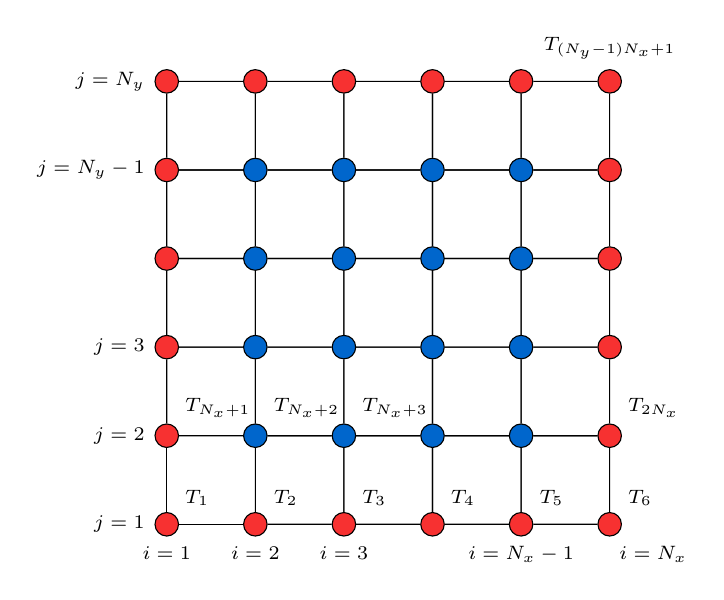
\begin{tikzpicture}[scale=0.75,font=\sffamily\scriptsize]
      \foreach \x in {0,...,5}
        \foreach \y in {0,...,5} 
          {
    %        \pgfmathtruncatemacro{\label}{\x - 5 *  \y +21}
          \ifthenelse{\x=0 \OR \x=5 \OR \y=0 \OR \y=5}{\node [gdot,fill=tuered]  (\x\y) at (1.5*\x,1.5*\y) {};}
          \node [gdot,fill=tueblue]  (\x\y) at (1.5*\x,1.5*\y) {};} 

        \foreach \x [count=\xi] in {0,...,4}
          \foreach \y [count=\yi] in {0,...,4}  
            \draw (\x\y)--(\x\yi)-- (\xi\yi)--(\xi\y)--(\x\y);% (\y\x)--(\yi\x) ;
        
        \onslide<2->{
	  \node[anchor=east] at (00.west) {$j=1$};
	  \node[anchor=east] at (01.west) {$j=2$};
	  \node[anchor=east] at (02.west) {$j=3$};
	  \node[anchor=east] at (04.west) {$j=N_y-1$};
	  \node[anchor=east] at (05.west) {$j=N_y$};
	  \node[anchor=north] at (00.south) {$i=1$};
	  \node[anchor=north] at (10.south) {$i=2$};
	  \node[anchor=north] at (20.south) {$i=3$};
	  \node[anchor=north] at (40.south) {$i=N_x-1$};
	  \node[anchor=north west] at (50.south) {$i=N_x$};
	}
	
	\onslide<3->{
	  \node[anchor=south west] at (00.north east) {$T_1$};
	  \node[anchor=south west] at (10.north east) {$T_2$};
	  \node[anchor=south west] at (20.north east) {$T_3$};
	  \node[anchor=south west] at (30.north east) {$T_4$};
	  \node[anchor=south west] at (40.north east) {$T_5$};
	  \node[anchor=south west] at (50.north east) {$T_6$};
	  \node[anchor=south west] at (01.north east) {$T_{N_x+1}$};
	  \node[anchor=south west] at (11.north east) {$T_{N_x+2}$};
	  \node[anchor=south west] at (21.north east) {$T_{N_x+3}$};
	  \node[anchor=south west] at (51.north east) {$T_{2N_x}$};
	  \node[anchor=south]      at (55.north) {$T_{(N_y-1)N_x+1}$};
	}
      \end{tikzpicture}
%     \end{center}
  \hfill
  \column{0.35\textwidth}
  \begin{itemize}
    \item<1-> Define a grid of points in $x$ and $y$
    \item<2-> Index of the grid points using 2D coordinates $i$ and $j$
    \item<3> Set up the equations using a 1D index system: $T_{i,j}=T_{i+N_x(j-1)}$
  \end{itemize}
  \end{columns}
\end{frame}

\begin{frame}[fragile]
  \frametitle{Discretization of Laplace's equation (II)}
  Estimate the second-order differentials: assume a piece-wise linear profile in the temperature: \vskip1em
  \begin{columns}
  \column{0.5\textwidth}
    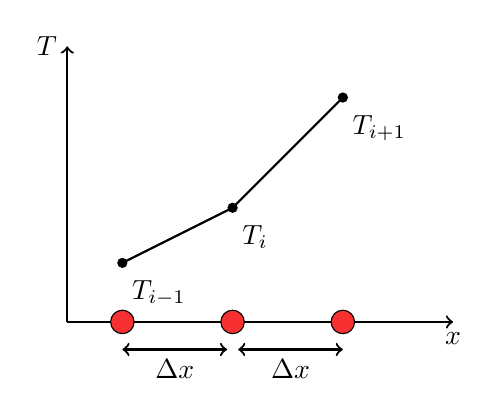
\begin{tikzpicture}[scale=0.7,node distance=5mm]
      \draw[black,thick,->] (0,0)-- node[at end,anchor=north]{$x$}(7,0);
      \draw[black,thick,->] (0,0)-- node[at end,anchor=east ]{$T$}(0,5);
      \node [gdot,fill=tuered] (n1) at (1,0) {};
      \node [gdot,fill=tuered] (n2) at (3,0) {};
      \node [gdot,fill=tuered] (n3) at (5,0) {};
      \node [anchor=south,dot,color=black,fill=black] (e1) at (1,1) {};
      \node [anchor=south,dot,color=black,fill=black] (e2) at (3,2) {};
      \node [anchor=south,dot,color=black,fill=black] (e3) at (5,4) {};
      \node [below=1mm of e1.center,anchor=north west] (e4) {$T_{i-1}$};
      \node [below=1mm of e2.center, anchor=north west] (e5) {$T_{i}$};
      \node [below=1mm of e3.center,anchor=north west] (e6) {$T_{i+1}$};
      \draw[black,thick] (e1.center) -- (e2.center) -- (e3.center);
      \draw[black,thick,<->] (1,-0.5) -- node[midway, below] {$\Delta x$} (2.9,-0.5);
      \draw[black,thick,<->] (3.1,-0.5) -- node[midway, below] {$\Delta x$} (5,-0.5);
      \end{tikzpicture}
%     \end{center}
  \hfill
  \column{0.35\textwidth}
  \pause
  \begin{align*}
    \frac{\partial^2T}{\partial x^2} \approx \frac{\left.\frac{\partial T}{\partial x}\right|_{i+\frac{1}{2}}-\left.\frac{\partial T}{\partial x}\right|_{i-\frac{1}{2}}}{\Delta x} \\[15pt]
    \approx \frac{ \frac{\left(T_{i+1,j}-T_{i,j}\right)}{\Delta x} - \frac{\left(T_{i,j}-T_{i-1,j}\right)}{\Delta x}}{\Delta x}\\[15pt]
    = \frac{T_{i+1,j}-2T_{i,j}+T_{i-1,j}}{(\Delta x)^2}
  \end{align*}
  \end{columns}
\end{frame}

\begin{frame}[fragile]
  \frametitle{Discretization of Laplace's equation (III)}
  The $y$-direction is derived analogously, so that the 2D Laplace's equation is discretized as:
  \[
    \frac{T_{i+1,j}-2T_{i,j}+T_{i-1,j}}{(\Delta x)^2} + \frac{T_{i,j+1}-2T_{i,j}+T_{i,j-1}}{(\Delta y)^2} = 0
  \]
  \pause
  Use a single index counter ${k=i+N_x(j-1)}$, so that the equation becomes:
  \[
    \frac{T_{k+1}-2T_k+T_{k-1}}{(\Delta x)^2} + \frac{T_{k+N_x}-2T_k+T_{k-N_x}}{(\Delta y)^2} = 0
  \]
  \pause
  For an equal spaced grid $\Delta x = \Delta y = 1$:
  \tikz{\node[emphblock, text width=\textwidth,]{\[
   T_{k-N_x} + T_{k-1} - 4T_k + T_{k+1} + T_{k+N_x} = 0
   \]
   \[
      \Rightarrow AT=b
   \]\vskip1ex
   %\Rightarrow T_k = \frac{T_{k-N_x} + T_{k-1} + T_{k+1} + T_{k+N_x}}{4}
  };}
\end{frame}

\section{Creating a sparse system}
\subsection*{A sparse matrix}
\againframe<2>{contents_lin3}
\begin{frame}[fragile]
  \frametitle{Creating the linear system}
  \vskip-1em
  \[
   T_{k-N_x} + T_{k-1} - 4T_k + T_{k+1} + T_{k+N_x} = 0
  \]
  Create a \emph{banded} matrix $A$: the main diagonal $k$ contains -4, whereas the bands at $k-1$, $k+1$, $k-N_x$ and $k+N_x$ contain a 1. Boundary cells just contain a 1 on the main diagonal so that the temperature is equal to $T_b$ (e.g. $T_1 = 1T_b$).\\
  \vskip1em
  \hspace*{8em}
  ${
    \begin{bmatrix}
      1 & 0 & 0 & 0 & 0 & 0 & 0 & 0 & \cdots & 0\\
      0 & 1 & 0 & 0 & 0 & 0 & 0 & 0 & \cdots & 0\\
    \vdots & \vdots & \vdots & \vdots & \vdots & \vdots & \vdots & \vdots & \ddots & \vdots\\
     \cdots & 1 & \cdots & 1 & -4 & 1 &\cdots & 1 & \ddots & 0\\
     0 & \cdots & 1 & \cdots & 1 & -4 & 1 &\cdots & 1 & \vdots\\
     \vdots & \vdots & \vdots & \vdots & \vdots & \vdots & \vdots & \vdots & \ddots & \vdots\\
     0 & 0 & 0 & 0 & 0 & 0 & 0 & 0 & 1 & 0\\
     0 & 0 & 0 & 0 & 0 & 0 & 0 & 0 & 0 & 1\\
    \end{bmatrix}
    \begin{bmatrix}
    T_1\\
    T_2\\
    \vdots\\
    T_k\\
    T_k+1\\
    \vdots\\
    T_{(N_y-1)N_x}\\
    T_{(N_y-1)N_x+1}
   \end{bmatrix} = 
   \begin{bmatrix}
    T_b\\
    T_b\\
    \vdots\\
    0\\
    0\\
    \vdots\\
    T_b\\
    T_b
   \end{bmatrix}}$
\end{frame}

\begin{frame}[fragile]
  \frametitle{Creating the linear system}
  \vskip-1em
  \[
   T_{k-N_x} + T_{k-1} - 4T_k + T_{k+1} + T_{k+N_x} = 0
  \]
  Create a \emph{banded} matrix \(A\) in Python, by setting the coefficients for the internal cells:
\begin{lstlisting}
import numpy as np
from scipy.sparse import diags

Nx = 5  # number of points along x direction
Ny = 5  # number of points in the y direction
Nc = Nx * Ny  # Total number of points

e = np.ones(Nc)
A = diags([e, e, -4*e, e, e], [-Nx, -1, 0, 1, Nx], shape=(Nc, Nc))
b = np.zeros(Nc)
\end{lstlisting}
The function \lstinline$diags$ uses the following arguments:
\begin{itemize}
   \item The coefficients that have to be put on the diagonals arranged as columns in a matrix
   \item The position of the bands with respect to the main diagonal
   \item Size of the resulting matrix (in our case square $N_xN_y \times N_xN_y$)
  \end{itemize}
\end{frame}

\begin{frame}[fragile]
  \frametitle{Matrix sparsity}
  \begin{columns}
  \column{0.5\textwidth}
  
  \begin{itemize}
   \item Let's check the matrix layout:
   \begin{lstlisting}
>> plt.spy(A)
   \end{lstlisting}
    \item This command shows the non-zero values of a matrix
    \item Apart from the main diagonal, there are offset bands!
  \end{itemize}
  \column{0.5\textwidth}
    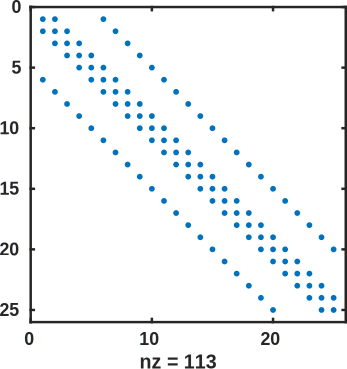
\includegraphics[width=\columnwidth]{sparse_matlab}
  \end{columns}
\end{frame}

\subsection*{Boundary conditions}
\begin{frame}[fragile]
  \frametitle{About boundary conditions}
  \begin{itemize}
    \item For the nodes on the boundary, we have a simple equation:
    \[
      T_{k,\text{boundary}} = \text{Some fixed value}
      \]
      \item However, we have set all nodes to be a function of their neighbors...
      \item Find the boundary node indices using $k = i + Nx(j-1)$
      \begin{itemize}
        \item \lstinline$i = 1$, \lstinline$j = 1:Ny$
        \item \lstinline$i = Nx$, \lstinline$j = 1:Ny$
        \item \lstinline$j = 1$, \lstinline$i = 1:Nx$
        \item \lstinline$j = Ny$, \lstinline$i = 1:Nx$
      \end{itemize}
      \item Reset the row in $A$ to zeros, set $A_{kk}$ = 1
      \item Set value in rhs: $b_k = T_{k,\text{boundary}}$
      \item Boundary conditions are often more elaborate to implement! See \lstinline$setBoundaryConditions.m$.
  \end{itemize}
\end{frame}
  
\begin{frame}[fragile]
  \frametitle{Partial implementation of the boundary conditions}
  See \lstinline$set_boundary_conditions.py$.
  \begin{lstlisting}[language=Python]
def set_boundary_conditions(A, b, Tb, Nx, Ny):
    # Set boundary conditions over x-direction
    for i in range(Nx):
        j = 0
        ind = i + Nx * j
        A[ind, :] = 0  # Reset matrix for boundary cells
        A[ind, ind] = 1  # Add a 1 on the diagonal
        b[ind] = Tb[0]
        
        j = Ny - 1
        ind = i + Nx * j
        A[ind, :] = 0  # Reset matrix for boundary cells
        A[ind, ind] = 1  # Add a 1 on the diagonal
        b[ind] = Tb[1]

    # Repeat for y-direction
    # ...
    return A, b
  \end{lstlisting}
\end{frame}

\begin{frame}[fragile]
  \frametitle{How applying boundary conditions affects the linear system}
  \begin{lstlisting}[language=Python]
def set_boundary_conditions(A, b, Tb, Nx, Ny):
  \end{lstlisting}
  \pause
  \begin{itemize}
    \item Make sure that matrix \lstinline$A$ and right hand side vector \lstinline$b$ are defined, as well as \lstinline$Nx$ and \lstinline$N_y$
    \item Create a vector that holds the temperature at each boundary:
    \begin{lstlisting}
>> T = [10, 20, 30, 40];
    \end{lstlisting}
    \item Call the function, store $A$ and $b$ in new variables:
    \begin{lstlisting}
>> A2,b2 = setBoundaryConditions(A,b,T,Nx,Ny);
    \end{lstlisting}
    \item Check the new structure of the matrix and the right hand side:
    \begin{lstlisting}
>> plt.subplot(121); plt.spy(A2);
>> plt.subplot(122); plt.spy(b2);
    \end{lstlisting}
  \end{itemize}
\end{frame}

\subsection*{Solving the equation}
\begin{frame}[fragile]
  \frametitle{A full program, including solver}
  The program and auxiliary functions are on Canvas (\lstinline$solve_laplace_eq.py$)
  \begin{lstlisting}[linewidth=1.05\textwidth]
from scipy.sparse import diags
import numpy as np
from scipy.sparse.linalg import spsolve
import matplotlib.pyplot as plt

def solve_laplace_eq(Nx, Ny):
    # Solves the steady-state Laplace equation
    
    Tb = [10, 20, 30, 40]  # Fixed boundary temperatures

    # Fill sparse matrix with [1, 1, -4, 1, 1]
    e = np.ones(Nx*Ny)
    A = diags([e, e, -4*e, e, e], [-Nx, -1, 0, 1, Nx], shape=(Nx*Ny, Nx*Ny))
    b = np.zeros(Nx*Ny)

    A, b = set_boundary_conditions(A, b, Tb, Nx, Ny)

    T = spsolve(A, b)  # Solve matrix
    Tc = T.reshape(Nx, Ny)  # Reshape x-vec to mat Nx, Ny
    xc, yc = np.meshgrid(range(Nx), range(Ny))  # Get position arrays
    plt.surf(xc, yc, Tc)  # Surface plot
    plt.show()

# Remember to define the set_boundary_conditions function before calling solve_laplace_eq
  \end{lstlisting}
\end{frame}

  
\begin{frame}[fragile]
  \frametitle{Sample results}
  Solved for a $20\times20$ system with $T_b=\left[10\ 20\ 30\ 40\right]$.\vskip1em
  \begin{center}
    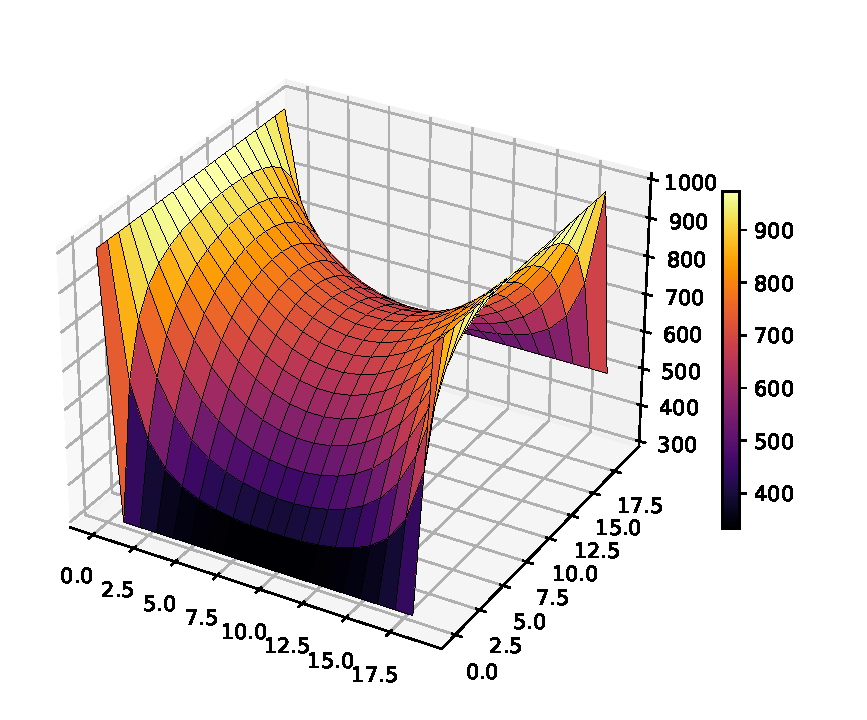
\includegraphics[width=0.6\textwidth]{laplace_20x20}
  \end{center}
\end{frame}

{\nologo
\begin{frame}[fragile]
  \frametitle{Exercise: Verify the numerical solution using Fourier-series}
  A Fourier-series expansion for the steady-state heat conduction in a flat plate is given for a domain: $x,y\in[0,1]$ , with fixed-temperature boundaries $T\big|_{x=0} = T\big|_{x=1} = T\big|_{y=0}=0$ and $T\big|_{y=1}=1$:
\[
    T = \frac{4}{\pi} \sum_{n=1}^\infty \frac{\sin\left(m \pi x \right)\sinh\left(m\pi y \right)}{m \sinh\left(m \pi \right)} \quad \text{with} \quad m=2n-1
\]
Compute and plot the exact temperature profile in the 2D plate, and compare it with the numerical solution:
  \begin{hints}
  Hints:
  \begin{itemize}
      \item Use meshgrid to create a mesh in $x$ and $y$
      \item Compute the temperature using the Fourier series, use vectorised computations over $x$ and $y$ so that only 1 loop (over n) is required.
      \item Solve the numerics for the same problem (note the boundary conditions)
      \item Compare the numerical and exact solutions (e.g. a plot).
  \end{itemize}
  \end{hints}
\end{frame}

\begin{frame}<beamer:1-|handout:0>[fragile]
  \frametitle{Exercise: Verify the numerical solution using Fourier-series}
    \begin{lstlisting}[language=Python]
import numpy as np
import matplotlib.pyplot as plt

Nx = 35; Ny = 35;
x, y = np.meshgrid(np.linspace(0,1,Nx), np.linspace(0,1,Ny))
T = np.zeros_like(x) # (*@ \pause @*)
# Fourier series expansion
for n in range(1,101):
    m = 2*n-1
    T += (np.sin(m*np.pi*x) * np.sinh(m*np.pi*y)) / (m * np.sinh(m*np.pi))
Tex = T * 4 / np.pi # (*@ \pause @*)
# Compute numerical solution and post-process

# First plot is created inside solve_laplace_eq, which also returns Tnum
fig, axs = plt.subplots(1, 3, figsize=(15, 5))
xc, yc, Tnum = solve_laplace_eq(Nx, Ny) 

# Plot exact (Fourier)
axs[1].plot_surface(x, y, Tex, cmap='viridis')
axs[1].set_xlabel('x'); axs[1].set_ylabel('y'); axs[1].set_zlabel('T')
# Plot difference
axs[2].plot_surface(x, y, Tex - Tnum, cmap='viridis')
axs[2].set_xlabel('x'); axs[2].set_ylabel('y'); axs[2].set_zlabel('T')
plt.show()
    \end{lstlisting}
\end{frame}
}

\begin{frame}[fragile]
  \frametitle{LU decomposition of a sparse matrix}
  \begin{columns}
  \column{0.35\textwidth}
    \begin{lstlisting}
>> [L,U,P] = lu(A)
>> plt.subplot(121)
>> plt.spy(L)
>> plt.subplot(122)
>> plt.spy(U)
    \end{lstlisting}
  \column{0.65\textwidth}
  \pause
  \begin{itemize}
    \item With LU decomposition we produce matrices that are less sparse than the original matrix.
    \item Sparse storage often required, and also numerical techniques that fully utilizes this!
  \end{itemize}\vskip2em
  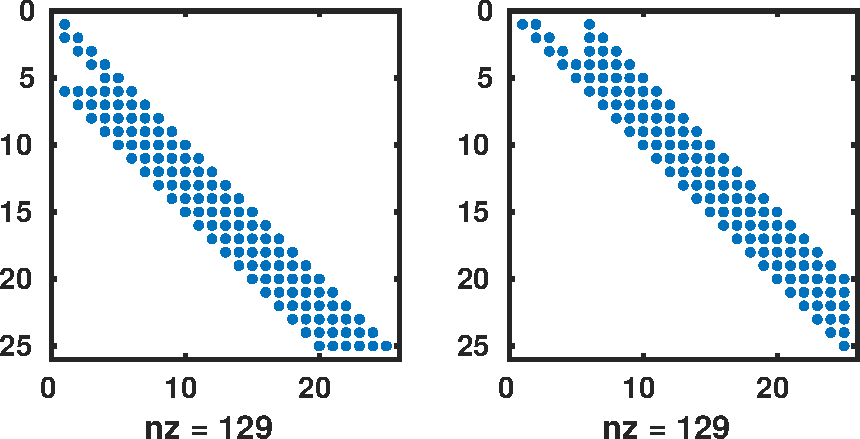
\includegraphics[width=\columnwidth]{sparse_lu}
  \end{columns}
\end{frame}
  
\begin{frame}[fragile]
  \frametitle{LU decomposition}
  \begin{itemize}
    \item LU decomposition and Gaussian elimination on a matrix like $A$ requires more memory (with 3D problems, the offset in the diagonal would even be bigger!)
    \item In general extra memory allocation will not be a problem for Python
    \item Python is clever, in that sense that it attempts to reorder equations, to move elements closer to the diagonal)
  \end{itemize} \pause
  Alternatives for elimination methods
  \begin{itemize}
    \item Use iterative methods when systems are large and sparse.
    \item Often such systems are encountered when we want to solve PDE’s of higher dimensions
  \end{itemize}
\end{frame}

\section{Iterative methods}
\subsection*{Introduction}
\againframe<2>{contents_lin3}

\begin{frame}[fragile]
  \frametitle{Examples of iterative methods}
  \begin{itemize}
    \item Jacobi method
    \item Gauss-Seidel method
    \item Succesive over relaxation \vskip2em
    \item \lstinline$bicg$ --- Bi-conjugate gradient method
  \item \lstinline$pcg$ --- preconditioned conjugate gradient method
  \item \lstinline$gmres$ --- generalized minimum residuals method
  \item \lstinline$bicgstab$ --- Bi-conjugate gradient method
\end{itemize}
\end{frame}

\subsection*{Jacobi method}
\begin{frame}[fragile]
  \frametitle{The Jacobi method}
  \begin{itemize}
     \item In our example we derived the following equation:
    \[
     T_{k-N_x} + T_{k-1} - 4T_k + T_{k+1} + T_{k+N_x} = 0
    \]
    \item Rearranging gives:
    \[
      T_k = \frac{T_{k-N_x} + T_{k-1} + T_{k+1} + T_{k+N_x}}{4}
    \]\pause
    \item In the Jacobi scheme the iteration proceeds as follows:
    \begin{enumerate}
      \setlength{\itemindent}{1cm}
      \item Start with an initial guess for the values of $T$ at each node\pause
      \item Compute updated values and store a new vector:
        \[
          T_k^\text{new} = \frac{T_{k-N_x}^\text{old} + T_{k-1}^\text{old} + T_{k+1}^\text{old} + T_{k+N_x}^\text{old}}{4}
        \]\pause
      \item Do this for all nodes\pause
      \item Repeat the procedure until converged
    \end{enumerate}
  \end{itemize}
\end{frame}

\begin{frame}[fragile]
  \frametitle{Jacobi method for Laplace's equation}
  \vskip-1em
  See \lstinline$laplace_jacobi.py$ (from Canvas)
  \begin{lstlisting}[language=Python,basicstyle=\scriptsize]
import numpy as np
import matplotlib.pyplot as plt
from matplotlib import cm

nx = 40; ny = 40; # (*@ \pause @*)
# The temperature field + boundaries at old and new times
T = np.zeros((nx, ny))
T[0, :] = 40;  # Left 
T[nx-1, :] = 60; # Right
T[:, 0] = 20;  # Bottom
T[:, ny-1] = 30; # Top # (*@ \pause @*)
Tnew = np.copy(T); # (*@ \pause @*)
# For plotting
x, y = np.meshgrid(range(nx), range(ny)); # (*@ \pause @*)

for iter in range(1000):
  for i in range(1, nx-1):
    for j in range(1, ny-1):
      Tnew[i, j] = (T[i-1, j] + T[i+1, j] + T[i, j-1] + T[i, j+1]) / 4.0;(*@ \pause @*)
  fig = plt.figure()
  ax = fig.add_subplot(111, projection='3d')
  ax.plot_surface(x, y, Tnew, cmap=cm.coolwarm)
  ax.set_title(f'Iteration: {iter}')
  plt.draw()
  plt.pause(0.01)
  T = np.copy(Tnew)  # Update T
  plt.close(fig)
    \end{lstlisting}
\end{frame}

\begin{frame}[fragile]
  \frametitle{About the straightforward implementation}
  \begin{itemize}
  
   \item The method as implemented works fine for a simple Laplace equation
%    \item We did not take into account the thermal diffusivity (set to unity)
%    \item We did not take into account the grid spacing (set to unity)
   \item For generic systems of linear equations, the implementation cannot be used.
  \end{itemize}\vskip2em\pause
 \tikz{\node[emphblock,text width=\textwidth]{We will now introduce the Jacobi method so it can be used for generic systems of linear equations.};}
\end{frame}

\begin{frame}[fragile]
  \frametitle{The Jacobi method with matrices}
  We can split our (banded) matrix $A$ into a diagonal matrix $D$ and a remainder $R$:\vskip1em
  \[
   A \quad =\quad  D \quad + \quad R
  \]
 \vskip2em
  \scalebox{0.6}{
  $
   \begin{bmatrix}
    \times & \times &  &  &  &  & \times &  & \\
    \times & \times & \times &   &   &   &   & \times &    \\
           & \times & \times & \times &   &   &   &   & \times \\
           &   & \times & \times & \times &   &   &   &   \\
      &   &   & \times & \times & \times &   &   &    \\
      &   &   &   & \times & \times & \times &   &   \\
      \times &   & &   &   & \times & \times & \times &   \\
      &   \times &   & &   &   & \times & \times & \times \\
      &   &   \times &   & &   &   & \times & \times \\
   \end{bmatrix} = 
   \begin{bmatrix}
    \times &  &  &  &  &  &  &  & \\
     & \times &  &   &   &   &   &  &    \\
           &  & \times &  &   &   &   &   &  \\
           &   &  & \times &  &   &   &   &   \\
     &   &   &  & \times &  &   &   &    \\
      &  &   &   &  & \times &  &   &   \\
      &   &  &   &   &  & \times &  &   \\
      &   &   &  &   &   &  & \times &  \\
      &   &   &   &  &   &   &  & \times \\
   \end{bmatrix} + 
   \begin{bmatrix}
     & \times &  &  &  &  & \times &  & \\
    \times &  & \times &   &   &   &   & \times &    \\
           & \times &  & \times &   &   &   &   & \times \\
           &   & \times &  & \times &   &   &   &   \\
      &   &   & \times &  & \times &   &   &    \\
      &   &   &   & \times &  & \times &   &   \\
      \times &   & &   &   & \times &  & \times &   \\
      &   \times &   & &   &   & \times &  & \times \\
      &   &   \times &   & &   &   & \times &  \\
   \end{bmatrix}$}
\end{frame}

\begin{frame}[fragile]
  \frametitle{Jacobi method: solving a system}
  \begin{itemize}
   \item We can solve $AT=b$, now written generally as $Ax=b$, by:
   \begin{align*}
      Ax&=b\\
     (D+R)x &= b \\
      Dx &= b -Rx \\
      Dx^\text{new} &= b - Rx^\text{old} \\
       x^\text{new} &= D^{-1}(b-Rx^\text{old})
   \end{align*}
   \item Using the $n$ and $n+1$ notation for old and new time steps, we find in general:
   \[
    x^{n+1} = D^{-1}\left(  b-Rx^n\right)
   \]
   \[
    x_i^{n+1} = \frac{1}{A_{ii}}\left(b_i - \sum_{j\neq i} A_{ij}x_j^n\right)
   \]
  \end{itemize}
\end{frame}

\begin{frame}[fragile]
  \frametitle{Diagram of the Jacobi method}
  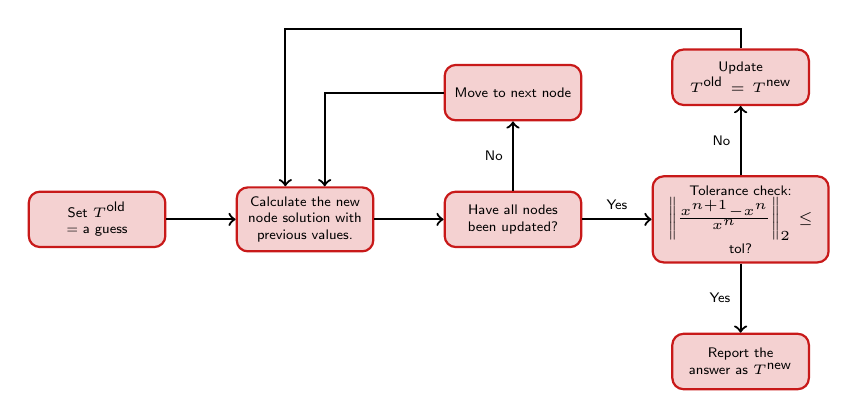
\begin{tikzpicture}[scale=0.5,font=\tiny,node distance = 25pt, auto,->=stealth,point/.style={circle,fill=red,minimum size=0pt,inner sep=0pt}]
    \tikzstyle{block2} = [rectangle,minimum height=1em,draw=maincolor,fill=maincolor!20,text centered,rounded corners,minimum height=2em,thick,text width=1.5cm]
    \node[block2]                 (start) {Set $T^\text{old}$ = a guess};
    \node[block2, right=of start,visible on=<2->] (calc)  {Calculate the new node solution with previous values.};
    \node[block2, right=of calc,visible on=<3->] (check1) {Have all nodes been updated?};
    \node[block2, right=of check1,,visible on=<5->,text width=2cm] (tol) {Tolerance check: $\mynorm{\frac{x^{n+1}-x^n}{x^n}}_2 \leq \text{tol} $?};
    \node[block2, above=of check1,visible on=<4->] (next) {Move to next node};
    \node[block2, above=of tol,visible on=<6->] (update) {Update $T^\text{old}=T^\text{new}$};
    \node[block2, below=of tol,visible on=<8->] (answer) {Report the answer as $T^\text{new}$};
    \draw[->,thick,black,visible on=<2->] (start.east) -- (calc.west);
    \draw[->,thick,black,visible on=<3->] (calc.east) -- (check1.west);
    \draw[->,thick,black,visible on=<5->] (check1.east) -- node[midway,above]{Yes} (tol.west);
    \draw[->,thick,black,visible on=<4->] (check1.north) -- node[midway]{No} (next.south);
    \draw[->,thick,black,visible on=<6->] (tol.north) -- node[midway,left] {No} (update.south);
    \draw[->,thick,black,visible on=<8->] (tol.south) -- node[midway,left] {Yes} (answer.north);
    \draw[->,thick,black,visible on=<7->] (update.north) |- ++(0,0.5cm) -| ($ (calc.north) + (-5mm,0)$);
    \draw[->,thick,black,visible on=<4->] (next.west) -| ($ (calc.north) + (5mm,0)$);
    
%     \draw[->,thick,black] (tol.north) -| ($ (digit.east) + (2mm,0) $) (calc.west);
%     \draw[->,thick,black] (start.east) -- (calc.west);
  \end{tikzpicture}
\end{frame}

\begin{frame}[fragile]
  \frametitle{The core of the solver}
  The full file is on Canvas, \lstinline$solve_jacobi.py$.
  \begin{lstlisting}[numbers=left]
import numpy as np

while (xDiff > tol and it_jac < 1000):
    x_old = np.copy(x)
    for i in range(N):
        s = 0
        for j in range(N):
            if j != i:
                s += A[i, j] * x_old[j]
        x[i] = (b[i] - s) / A[i, i]
    it_jac += 1
    xDiff = np.linalg.norm((x - x_old) / x, ord=2)

it_jac
  \end{lstlisting}
  \pause
  Try to call it from the \lstinline$solve_laplace_eq.py$ file, instead of using \lstinline$\$.
\end{frame}


\begin{frame}[fragile]
  \frametitle{A few details on this algorithm}
  \begin{itemize}
   \item The while loop holds two aspects
   \begin{itemize}
    \item A convergence criterion (\lstinline$norm((x-x_old)./x) > tol$). Some considerations are:
    \begin{itemize}
      \item $L_1$-norm (sum)
      \item $L_2$-norm (Euclidian distance)
      \item $L_\infty$-norm (max)
    \end{itemize}
    \item Protection against infinite loops (no convergence)
   \end{itemize}\pause
   \item Reset the sum for each row, before summing for the new unknown node
  \end{itemize}\pause
  \vskip1em
  \begin{itemize}
    \item Start vector x is not shown in the example, but should be there!
    \item It can have huge impact on performance!
    \item The for-loops also have a large performance penalty!
  \end{itemize}
\end{frame}

\begin{frame}[fragile]
  \frametitle{The solver using array indices}
  Make a copy of the Jacobian solver, and replace the for-loop by a vector-operation:
  \begin{lstlisting}[basicstyle=\scriptsize\ttfamily]
# While not converged or max_it not reached
import numpy as np

while ( xDiff > tol and it_jac < 1000 ):
  x_old = np.copy(x)
  for i in range(N):
    # Sum off-diagonal*x_old
    offDiagonalIndex = np.concatenate((np.arange(0, i), np.arange(i+1, N)))
    Aij_Xj = np.dot(A[i, offDiagonalIndex], x_old[offDiagonalIndex])

    # Compute new x value
    x[i] = (b[i] - Aij_Xj) / A[i, i]
  it_jac += 1
  xDiff = np.linalg.norm((x - x_old) / x, ord=2)
\end{lstlisting}
\end{frame}


\begin{frame}[fragile]
  \frametitle{Iterations 1, 2, 3 and 10}
  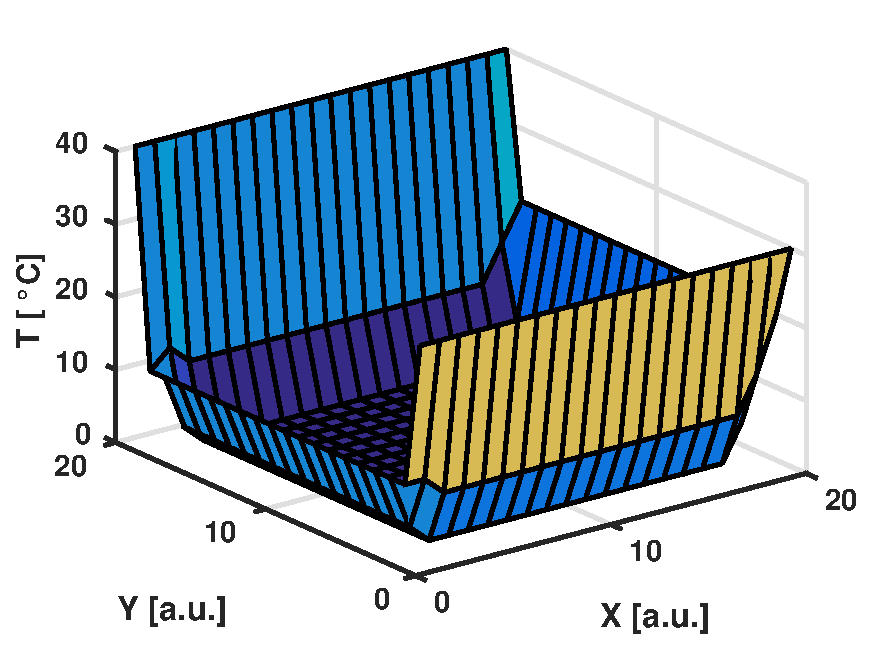
\includegraphics[width=0.35\textwidth]{it1} \hspace{0.5cm}
  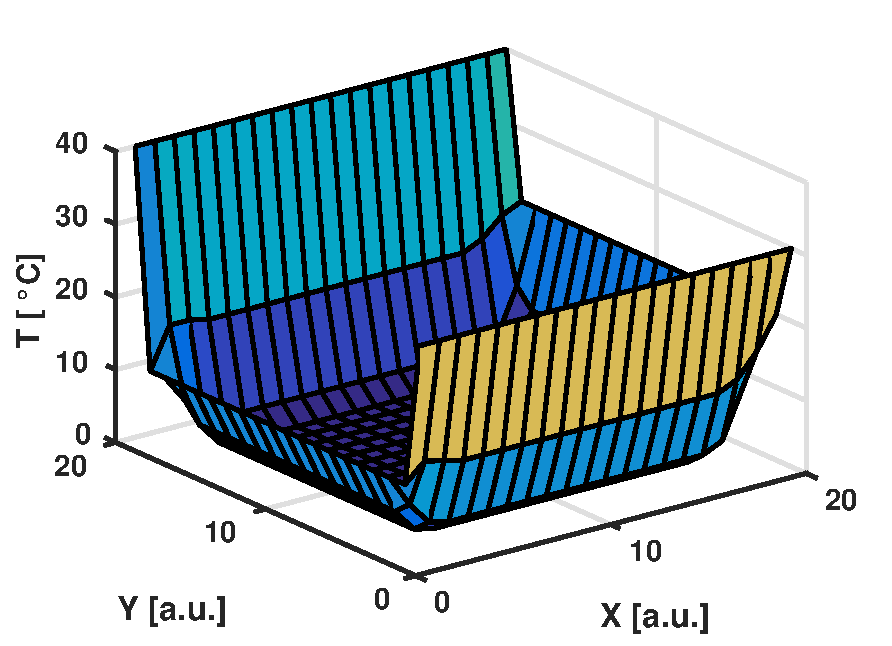
\includegraphics[width=0.35\textwidth]{it2}\\
  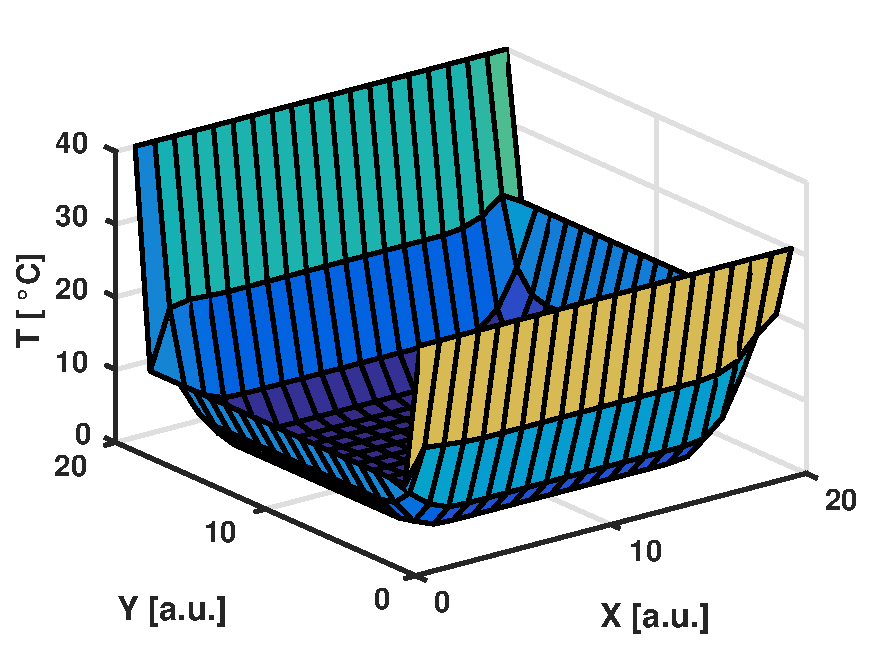
\includegraphics[width=0.35\textwidth]{it3} \hspace{0.5cm} 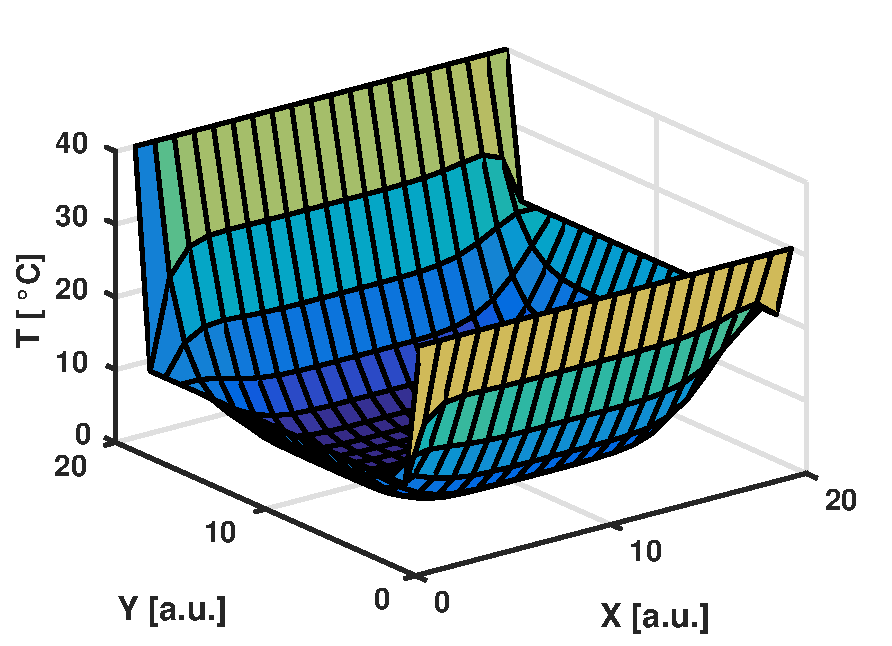
\includegraphics[width=0.35\textwidth]{it10}
\end{frame}

\subsection*{Gauss-Seidel method}
\begin{frame}[fragile]
  \frametitle{Gauss-Seidel method}
  The Gauss-Seidel method is quite similar to Jacobi method
  \begin{itemize}
   \item The only difference is that the new estimate $x^\text{new}$ is returned to the solution $x^\text{old}$ as soon as it is completed
   \item For following nodes, the updated solution is used immediately \pause
   \item Our straightforward script (from the Jacobi method) is therefore changed easily:
   \begin{itemize}
    \item Do not create a \lstinline$Tnew$ array (save memory!)
    \item Do not store the solution in \lstinline$Tnew$, but simply in \lstinline$T$
    \item Do not perform the update step \lstinline$T=Tnew$
    \item See \lstinline$laplace_gaussseidel.m$ for the algorithm.\pause
   \end{itemize}
   \item The straightforward script works well for the current Laplace equation, but we define the generic Gauss-Seidel algorithm on the following slides.
  \end{itemize}
\end{frame}

\begin{frame}[fragile]
  \frametitle{Gauss-Seidel method}
  \begin{itemize}
    \item Define a lower and strictly upper triangular matrix, such that $A = L + U$
    \item Now we can solve AT=b by:
    \begin{align*}
      (L+U)T &= b \\
      LT &= b - UT \\
      LT^\text{new} &= b - UT^\text{old} \\
      T^\text{new} &= L^{-1}(b-UT^\text{old})
   \end{align*}
     \item Using the $n$ and $n+1$ notation for old and new time steps, we find in for the general Gauss-Seidel method:
     \[
      x^{n+1} = L^{-1}\left(b-Ux^n\right)
     \]
     \[
      x_i^{n+1} = \frac{1}{A_{ii}}\left(b_i - \sum_{j<i} A_{ij}x_j^{n+1}- \sum_{j>i} A_{ij}x_j^n\right)
     \]
  \end{itemize}
\end{frame}

\section{Summary}
\subsection*{Summary}
\againframe<2>{contents_lin3}
\begin{frame}[fragile]
  \frametitle{Summary}
  \begin{itemize}
    \item Partial differential equations can be discretized into sparse systems of linear equations
    \item Sparse matrices can be stored in memory efficiently using specialised formats (e.g. compressed row storage)
    \item The Jacobi and Gauss–Seidel methods were introduced as iterative methods; other methods are based on the same principle (successive over-relaxation method, for example)
    \item Various implementation issues were discussed, e.g. vectorised computing, convergence tolerances
  \end{itemize}
\end{frame}

\begin{frame}[fragile]
  \frametitle{Direct methods vs. Iterative methods}
  \begin{itemize}
    \item Iterative methods converge \emph{gradually} to a solution while direct methods (possibly with partial pivoting) factorise a (set of) matrix(ces) which allow to compute the solution by \emph{substitution}.
    \item Direct methods generally use more memory, since they need to store also the result matrices.
    \item A strictly (or irreducibly) diagonally dominant matrix is a prerequisite for convergence of the Jacobi and Gauss-Seidel method.
    \item For real-life situations; 1D problems are generally solved with direct methods (LU decomposition). If you have systems of more than 1 dimension, a direct method still can be used, if there are no memory issues, otherwise an iterative method would be more attractive.
\end{itemize}
\end{frame}

\title{Numerical interpolation}
\subtitle{}
\lecture{interpolation}{interpolation}
\part{Numerical interpolation}
% \frame{\partpage}
\section{Introduction}
\subsection*{General}
\begin{frame}[label=contents_interpolation]
  \frametitle{Today's outline}
  \mode<beamer>{
    \only<1>{\tableofcontents}
  }
  \only<2>{\tableofcontents[currentsection,currentsubsection]}
\end{frame}

\begin{frame}
  \frametitle{Interpolation problem}
  \begin{definition}
  Given a set of points $x_k$, $k=0,\ldots,n$, $x_i \neq x_j$ with associated function values $f_k$, $k=0,\ldots,n$, or simply: $\{x_k,f_k\}_{k=0}^n$. The interpolation problem is defined as: find a polynomial $p_n$ such that this interpolates the values of $f_k$ on the points $x_k$:
  \[
    p_n(x_k)=f_k, \quad k=0,\ldots,n
  \]
  \end{definition}
  \pause
  \begin{theorem}
    The interpolation problem for $\{x_k,f_k\}_{k=0}^n$ has a unique solution when $x_i \neq x_j$ for $i \neq j$. Note that we cannot allow multiple function values $f_k$ for the same value of $x_k$.
  \end{theorem}
\end{frame}

\frame{
  \frametitle{What is interpolation?}
  \vfill
  \tikz{\node[emphblock,text width=\textwidth] 
    {
    Interpolation means constructing additional data points within the range of, and using, a discrete set of known data points.
    \vskip1em
    It is typically performed on a uniformly spread data set, but this is not strictly necessary for all methods
    };}
  \vfill
}
\frame{
\frametitle{Is interpolation the same as curve fitting?}
\pause
\vfill
{\begin{center} \huge NO \end{center}}
\pause
\vfill
\begin{itemize}
  \colorize<3> \item Curve-fitting requires additionally some way of computing the error between function (curve) and data
  \colorize<4> \item Curve-fitting does not strictly enforce the function to match the data exactly
  \colorize<5> \item Curve-fitting may be done on multiple datapoints at one position
  \colorize<6> \item Curve-fitting is much more expensive to do, requires optimisation
\end{itemize}
\vfill
}

\begin{frame}
  \frametitle{Why do chemical engineers need interpolation?}
  \begin{itemize}
    \colorize<1> \item Comparison of two data sets which are given at different positions
    \begin{itemize}
     \colorize<1> \item An experimental data set may have been recorded at a constant rate, but the numerical solution is computed at irregular intervals
    \end{itemize}
    \colorize<2> \item Reconstruction of field values distant of computing nodes
    \begin{itemize}
      \colorize<2> \item A CFD simulation on a regular grid containing structures that are not grid-conformant requires interpolation to the structures
    \end{itemize}
    \colorize<3> \item Calculation of a physical property at a condition between those of a lookup table
    \begin{itemize}
      \colorize<3> \item The viscosity of a substance may have been measured at 20\si{\celsius} and 30\si{\celsius}, but not at the desired 28.5\si{\celsius}
    \end{itemize}
  \end{itemize}
\end{frame}

%'exp(-x)+8*sin(x)+2*x'

\frame{
  \frametitle{General}
  Several important numerical interpolation methods are discussed today:
  \vskip2em
  \begin{itemize}
  \item Piecewise constant interpolation
  \item Linear interpolation
  \begin{itemize}
    \item Bilinear interpolation
  \end{itemize}
  \item Polynomial interpolation (Newton's method)
  \item Spline interpolation
  \end{itemize}
}

\section{Piecewise constant}
\subsection*{}
\againframe<2>{contents_interpolation}
\begin{frame}
  \frametitle{Today's data set}
  \footnotesize\selectfont
  \begin{columns}
    \column{0.45\textwidth}
    Download the datafile \lstinline$interpolation-dataset.txt$, which contains multiple data sets.\vskip2em\pause
    \begin{center}
      We start with \lstinline$x1$ and \lstinline$y1$:\vskip1em
      \begin{tabular}{c|r}
	$x_k$ & $f_k$ \\ \hline
	$0$ & $1.00$ \\
	$1$ & $\frac{11}{3}=3.67$ \\
	$2$ & $\frac{8}{3}=2.67$  \\
	$3$ & $1.00$ \\
	$4$ & $\frac{5}{3}=1.67$  \\
	$5$ & $\frac{23}{3}=7.67$ \\ \hline
      \end{tabular}
    \end{center}
    \column{0.55\textwidth}
    Data set $f_n(x_n)$ represented by \tikz{\node[interp]{};} at discrete intervals $x_n\in\{0,5\}$
    \vskip1em
    \centering
    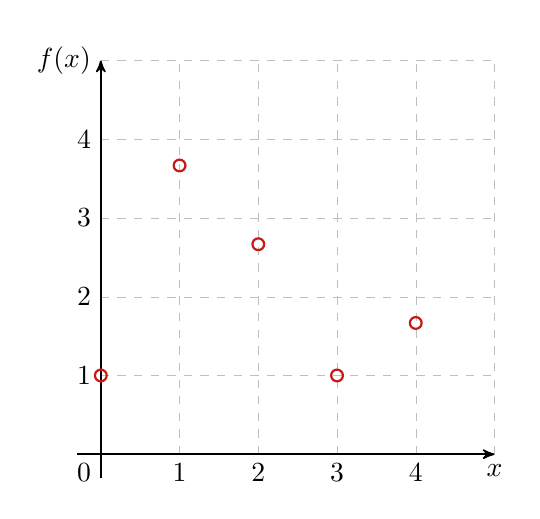
\begin{tikzpicture}[domain=-1:6]
        \draw[gridline,step=1] (0,0) grid (5,5);
  \coordinate (O) at (0,0);
  % Axes
  \draw[line,->] (-0.3,0) -- (5,0) coordinate[label = {below:$x$}] (xmax);
  \draw[line,->] (0,-0.3) -- (0,5) coordinate[label = {left:$f(x)$}] (ymax);
  
  % Labels
  \draw (0,0) node[below left]{$0$};
  \foreach \s in {1,...,4}
  {
    \draw (\s,0) node[below]{$\s$};
    \draw (0,\s) node[left]{$\s$};
    }
    
    % Title
    %       \draw (2.5,5) node[above]{$f(x)=\frac{x^3}{2}-\frac{10x^2}{3}+\frac{11x}{2}+1$};
    
    % Plots
    \node[interp] (x0) at (0,1) {};
    \node[interp] (x1) at (1,3.667) {};
    \node[interp] (x2) at (2,2.667) {};
    \node[interp] (x3) at (3,1) {};
    \node[interp] (x4) at (4,1.667) {};
    \node (bb) at (5,5.3) {};
%       \draw [graph,domain=0:4.69] plot (\x, {0.5*\x*\x*\x-(10/3)*\x*\x+5.5*\x+1});
%       \draw [graph,opacity=0.4,dashed,domain=-0.15:4.73] plot (\x, {0.5*\x*\x*\x-(10/3)*\x*\x+5.5*\x+1});

    \end{tikzpicture}
  \end{columns}
\end{frame}

\begin{frame}
  \frametitle{Piecewise constant interpolation}
  \footnotesize\selectfont
  \begin{columns}
    \column{0.45\textwidth}
%     \begin{overlayarea}{\columnwidth}{8cm}
      \begin{itemize}
	\colorize<2> \item Nearest-neighbor interpolation in the continuous range $x\in\left[0,5\right]$
	\colorize<3> \item How to treat the point halfway (e.g. at $x=2.5$)?
% 	\hspace*{-2em}
	\begin{flalign*}
	  x \in &[0, 0.5] &\rightarrow f(x) = f(0) & \\
	  x \in &[0.5, 1.5] &\rightarrow f(x) = f(1) & \\
	  x \in &[1.5, 2.5] &\rightarrow f(x) = f(2) & \\
	  x \in &[2.5, 3.5] &\rightarrow f(x) = f(3) & \\
	  x \in &[3.5, 4.5] &\rightarrow f(x) = f(4) &
	\end{flalign*}
	\vspace*{-1em}
	\colorize<4> \item Not often used for simple problems, but e.g. for 2D (Voronoi)
      \end{itemize}
%     \end{overlayarea}
    \column{0.55\textwidth}
    Data set $f_n(x_n)$ represented by \tikz{\node[interp]{};} at discrete intervals $x_n\in\{0,5\}$
    \vskip1em
    \centering
    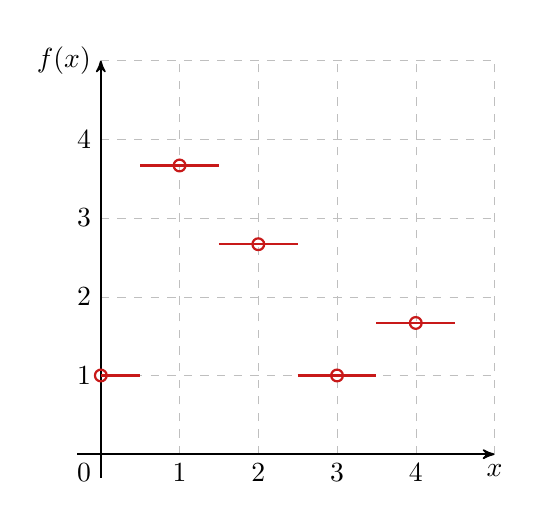
\begin{tikzpicture}[domain=-1:6]
        \draw[gridline,step=1] (0,0) grid (5,5);
  \coordinate (O) at (0,0);
  % Axes
  \draw[line,->] (-0.3,0) -- (5,0) coordinate[label = {below:$x$}] (xmax);
  \draw[line,->] (0,-0.3) -- (0,5) coordinate[label = {left:$f(x)$}] (ymax);
  
  % Labels
  \draw (0,0) node[below left]{$0$};
  \foreach \s in {1,...,4}
  {
    \draw (\s,0) node[below]{$\s$};
    \draw (0,\s) node[left]{$\s$};
    }
    
    % Title
    %       \draw (2.5,5) node[above]{$f(x)=\frac{x^3}{2}-\frac{10x^2}{3}+\frac{11x}{2}+1$};
    
    % Plots
    \node[interp] (x0) at (0,1) {};
    \node[interp] (x1) at (1,3.667) {};
    \node[interp] (x2) at (2,2.667) {};
    \node[interp] (x3) at (3,1) {};
    \node[interp] (x4) at (4,1.667) {};
    \node (bb) at (5,5.3) {};
%       \draw [graph,domain=0:4.69] plot (\x, {0.5*\x*\x*\x-(10/3)*\x*\x+5.5*\x+1});
%       \draw [graph,opacity=0.4,dashed,domain=-0.15:4.73] plot (\x, {0.5*\x*\x*\x-(10/3)*\x*\x+5.5*\x+1});


      % Piecewise interpolant
      \draw<2->[interp] (0,1) -- (0.5,1);
      \draw<2->[interp] (0.5,3.667) -- (1.5,3.667);
      \draw<2->[interp] (1.5,2.667) -- (2.5,2.667);
      \draw<2->[interp] (2.5,1)     -- (3.5,1);
      \draw<2->[interp] (3.5,1.667) -- (4.5,1.667);
    \end{tikzpicture}
  \end{columns}
\end{frame}

\section{Linear}
\subsection*{}
\againframe<2>{contents_interpolation}
\begin{frame}
  \frametitle{Linear interpolation}
  \footnotesize\selectfont
  \begin{columns}
    \column{0.45\textwidth}
    \begin{itemize}
      \colorize<2> \item Linear interpolation to $(x,y)$ between 2 data points $(x_2,y_2)$ and $(x_3,y_3)$:
      \colorize<3> {\[ {\color<3>{tuegreen}\frac{y-y_2}{x-x_2}}=\color<3>{tuered}\frac{y_3-y_2}{x_3-x_2} \] }
      \colorize<4> \item Reordered, and more formally: 
      \[ y = y_n + (y_{n+1} - y_n)\frac{x-x_n}{x_{n+1}-x_n} \]
    \end{itemize}
    \column{0.55\textwidth}
    Data set $f_n(x_n)$ represented by \tikz{\node[interp]{};} at discrete intervals $x_n\in\{0,5\}$
    \vskip1em
    \centering
    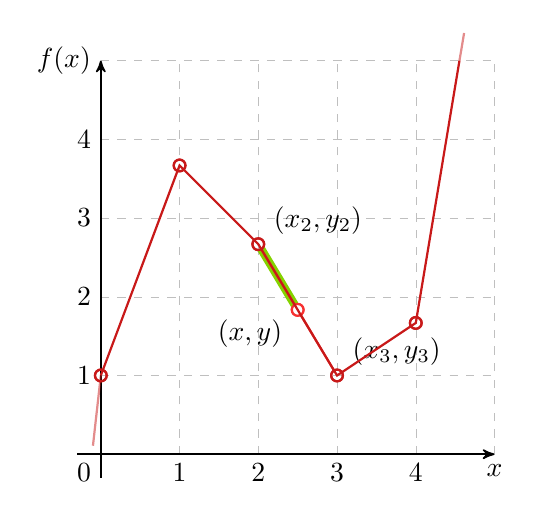
\begin{tikzpicture}[domain=-1:6]
        \draw[gridline,step=1] (0,0) grid (5,5);
  \coordinate (O) at (0,0);
  % Axes
  \draw[line,->] (-0.3,0) -- (5,0) coordinate[label = {below:$x$}] (xmax);
  \draw[line,->] (0,-0.3) -- (0,5) coordinate[label = {left:$f(x)$}] (ymax);
  
  % Labels
  \draw (0,0) node[below left]{$0$};
  \foreach \s in {1,...,4}
  {
    \draw (\s,0) node[below]{$\s$};
    \draw (0,\s) node[left]{$\s$};
    }
    
    % Title
    %       \draw (2.5,5) node[above]{$f(x)=\frac{x^3}{2}-\frac{10x^2}{3}+\frac{11x}{2}+1$};
    
    % Plots
    \node[interp] (x0) at (0,1) {};
    \node[interp] (x1) at (1,3.667) {};
    \node[interp] (x2) at (2,2.667) {};
    \node[interp] (x3) at (3,1) {};
    \node[interp] (x4) at (4,1.667) {};
    \node (bb) at (5,5.3) {};
%       \draw [graph,domain=0:4.69] plot (\x, {0.5*\x*\x*\x-(10/3)*\x*\x+5.5*\x+1});
%       \draw [graph,opacity=0.4,dashed,domain=-0.15:4.73] plot (\x, {0.5*\x*\x*\x-(10/3)*\x*\x+5.5*\x+1});

      
      % Interpolant points and captions
      \draw<2->[dot,draw=none] (x2) -- node[interp,color=tuered,midway,fill=white] (xy){} (x3);
      \node<2->[anchor=north east] at (xy.west) {$(x,y)$};
      \node<2->[anchor=south west] at (x2.east) {$(x_2,y_2)$};
      \node<2->[anchor=south west] at (x3.east) {$(x_3,y_3)$};
      % Slopes between the points in colors
      \draw<3>[dot,draw=tuegreen,line width=3pt] (x2) -- (xy);
      \draw<3->[dot] (x2) -- node[interp,color=tuered,midway,fill=white] (xy){} (x3);

      % Linear interpolant
      \draw<4->[interp] (0,1) node[interp]{} -- (1,3.667) node[interp]{} -- (2,2.667) node[interp]{} -- (3,1) node[interp]{} -- (4,1.667) node[interp]{} -- (4.555,5);
      \draw<4->[interp,opacity=0.5] (4.555,5) --(4.61388,5.35);
      \draw<4->[interp,opacity=0.5] (0,1) -- (-0.1,0.108);
    \end{tikzpicture}
  \end{columns}
\end{frame}

\begin{frame}
  \frametitle{Linear interpolation}
  \begin{itemize}
    \colorize<1> \item While linear interpolation is fast, and relatively easy to program, it is not very accurate
    \colorize<2> \item At the nodes, the derivatives are discontinuous i.e. not differentiable
    \colorize<3> \item Error is proportional to the square of the distance between nodes
  \end{itemize}
\end{frame}

\begin{frame}[t,fragile]
  \frametitle{Example: Linear interpolation in Python}
  \footnotesize\selectfont
  Consider the data set in \lstinline$sim_exp_dataset.mat$, containing a normalized concentration and time vector for an experiment and a simulation. The simulation was performed with adaptive node distance to save computation time, thus the concentration is not known at the same times. We are not able to compare yet.
  \vfill
  \begin{tikzpicture}
    \begin{axis}[
        width=\textwidth, height=5.5cm,     % size of the image
        grid = major,
        grid style={dashed, gray!30},
        %xmode=log,log basis x=10,
        %ymode=log,log basis y=10,
        xmin=0,     % start the diagram at this x-coordinate
        xmax=200,    % end   the diagram at this x-coordinate
        ymin=0,     % start the diagram at this y-coordinate
        ymax=0.02,   % end   the diagram at this y-coordinate
        /pgfplots/xtick={0,25,...,200}, % make steps of length 5
        /pgfplots/ytick={0.005,0.01,...,0.02}, % make steps of length 5
        axis background/.style={fill=white},
        ylabel=Concentration (\si{\mol\per\cubic\meter}),
        xlabel=Time (\si{\second}),
        tick align=outside,
        legend style={draw=none,fill=none}]

      % import the correct data from a CSV file
      \addplot[draw=tuered,mark=*,mark options={fill=white},mark size=0.7pt] table [id=exp]{student-data/exp_data.txt};
      \addlegendentry{Experiment};
      \addplot[draw=tueblue,mark=triangle*,mark options={fill=white},mark size=0.7pt] table [id=sim]{student-data/sim_data.txt};
      \addlegendentry{Simulation};
      % plot the stirling-formulae
%       \addplot[domain=0:60, red, thick] {1-(365/(365-x))^(365.5-x)*e^(-x)}; 
    \end{axis} 
\end{tikzpicture}
\end{frame}

\begin{frame}[t,fragile]
  \frametitle{Example: Linear interpolation in Python}
  \footnotesize\selectfont
  Consider the data set in \lstinline$sim_dataset.txt$ and \lstinline$exp_dataset.txt$, containing a normalized concentration and time vector for an experiment and a simulation. The simulation was performed with adaptive node distance to save computation time, thus the concentration is not known at the same times. We are not able to compare yet.
  \vfill
 \begin{columns}
  \column{0.49\textwidth}
  \begin{lstlisting}[language=Python,basicstyle=\tiny]
import numpy as np
import matplotlib.pyplot as plt

t_sim, c_sim = np.loadtxt("./student-data/sim_data.txt").T
t_exp, c_exp = np.loadtxt("./student-data/exp_data.txt").T

# Linear interpolation
c_sim_new = np.interp(t_exp, t_sim, c_sim)
diff = np.abs(c_exp - c_sim_new)

# Plot the solution
plt.subplot(2, 1, 1)
plt.plot(t_exp, c_exp, 'b-x', label='c_exp')
plt.plot(t_exp, c_sim_new, 'r-o', label='c_sim_new')
plt.legend()

plt.subplot(2, 1, 2)
plt.plot(t_exp, diff); plt.show()

# Compute the L2-norm
norm = np.linalg.norm(diff)
print(norm)
  \end{lstlisting}
  \column{0.5\textwidth}
  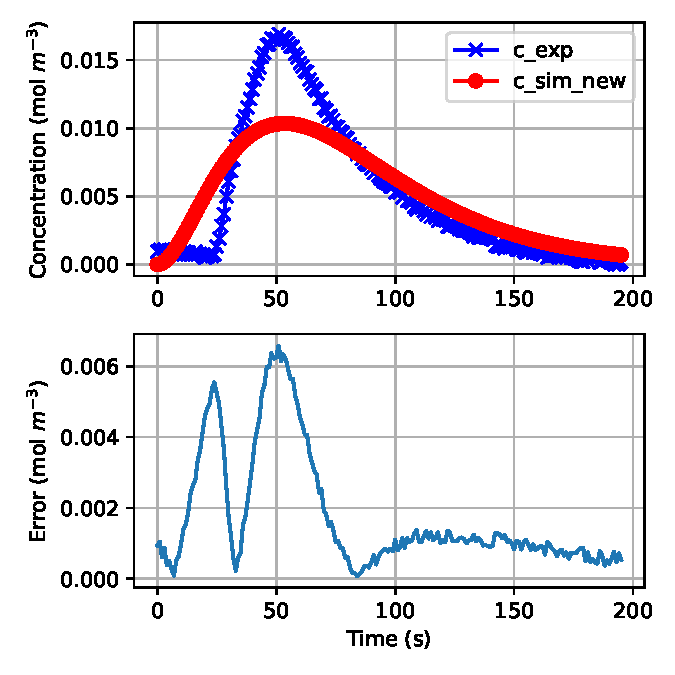
\includegraphics[width=0.8\textwidth]{sim_exp_data_interp.pdf}
\end{columns}
\end{frame}



\begin{frame}
  \frametitle{Bi-linear interpolation}
  When a 2D field of some quantity is known, we can interpolate the solution to an arbitrary position in the 2D domain $p(x,y)$ using 4 field values $f_{00}$, $f_{10}$, $f_{01}$ and $f_{11}$.
  \begin{columns}
    \column{0.5\textwidth}
      \colorize<3> 
      \begin{align*}
	g_1 &= f_{01}\frac{x_1-x}{x_1-x_0} + f_{11}\frac{x-x_0}{x_1-x_0} \\
	    &= f_{01}\frac{x_1-x}{\Delta x} + f_{11}\frac{x-x_0}{\Delta x}
      \end{align*}
      \colorize<4> 
      \[
	g_2 = f_{00}\frac{x_1-x}{\Delta x} + f_{10}\frac{x-x_0}{\Delta x}
      \]
      \colorize<5> 
      \[
	p = g_2\frac{y_1-y}{\Delta y} + g_1\frac{y-y_0}{\Delta y}
      \]
    \column{0.5\textwidth}
      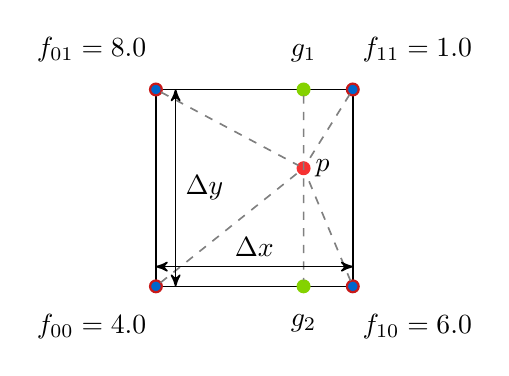
\begin{tikzpicture}[scale=2.5]
	\draw[line,-,step=1] (0,0) grid (1,1);
	\coordinate (O) at (0,0);
	\node[interp,fill=tueblue] (x0) at (0,0) {};
	\node[interp,fill=tueblue] (x1) at (1,0) {};
	\node[interp,fill=tueblue] (x2) at (1,1) {};
	\node[interp,fill=tueblue] (x3) at (0,1) {};
	\node<3->[interp,draw=tuegreen,fill=tuegreen] (g1) at (0.75,1) {};
	\node<4->[interp,draw=tuegreen,fill=tuegreen] (g2) at (0.75,0) {};
	
	\node[interp,draw=tuered,fill=tuered] (p) at (0.75,0.6) {};
	
	\node[below=1ex of x0,anchor=north east] {$f_{00}=4.0$};
	\node[below=1ex of x1,anchor=north west] {$f_{10}=6.0$};
	\node[above=1ex of x2,anchor=south west] {$f_{11}=1.0$};
	\node[above=1ex of x3,anchor=south east] {$f_{01}=8.0$};
	\node[right=-0.3ex of p] {$p$};
	\node<3->[above=1ex of g1] {$g_1$};
	\node<4->[below=1ex of g2] {$g_2$};
	\draw<2>[line,dashed,gray] (x0)--(p);
	\draw<2>[line,dashed,gray] (x1)--(p);
	\draw<2>[line,dashed,gray] (x2)--(p);
	\draw<2>[line,dashed,gray] (x3)--(p);
	\draw<5->[line,-,dashed,gray] (g1)--(g2);
	
	\draw[line,stealth'-stealth'] ($(x0)+(0,0.1)$) -- node[midway,above]{$\Delta x$}($(x1)+(0,0.1)$);
	\draw[line,stealth'-stealth'] ($(x0)+(0.1,0)$) -- node[midway,right]{$\Delta y$}($(x3)+(0.1,0)$);
      \end{tikzpicture}
  \end{columns}
  \onslide<6>{ \vskip1em
  \begin{itemize}
    \item The order of interpolation ($x$ or $y$ direction first) does not matter; the results are equal
  \end{itemize}
  }
\end{frame}

\begin{frame}
  \frametitle{Higher-dimensional field interpolation in Python}
  2D or higher-dimensional fields of data can be interpolated in Python using the \lstinline$scipy.interpolate.interp2d$, \lstinline$scipy.interpolate.interp3d$, or even \lstinline$scipy.interpolate.RegularGridInterpolator$ functions. The method can be adjusted:
  \vskip1em
  \begin{columns}
    \column{0.33\textwidth}
      \centering
      \lstinline$'nearest'$
      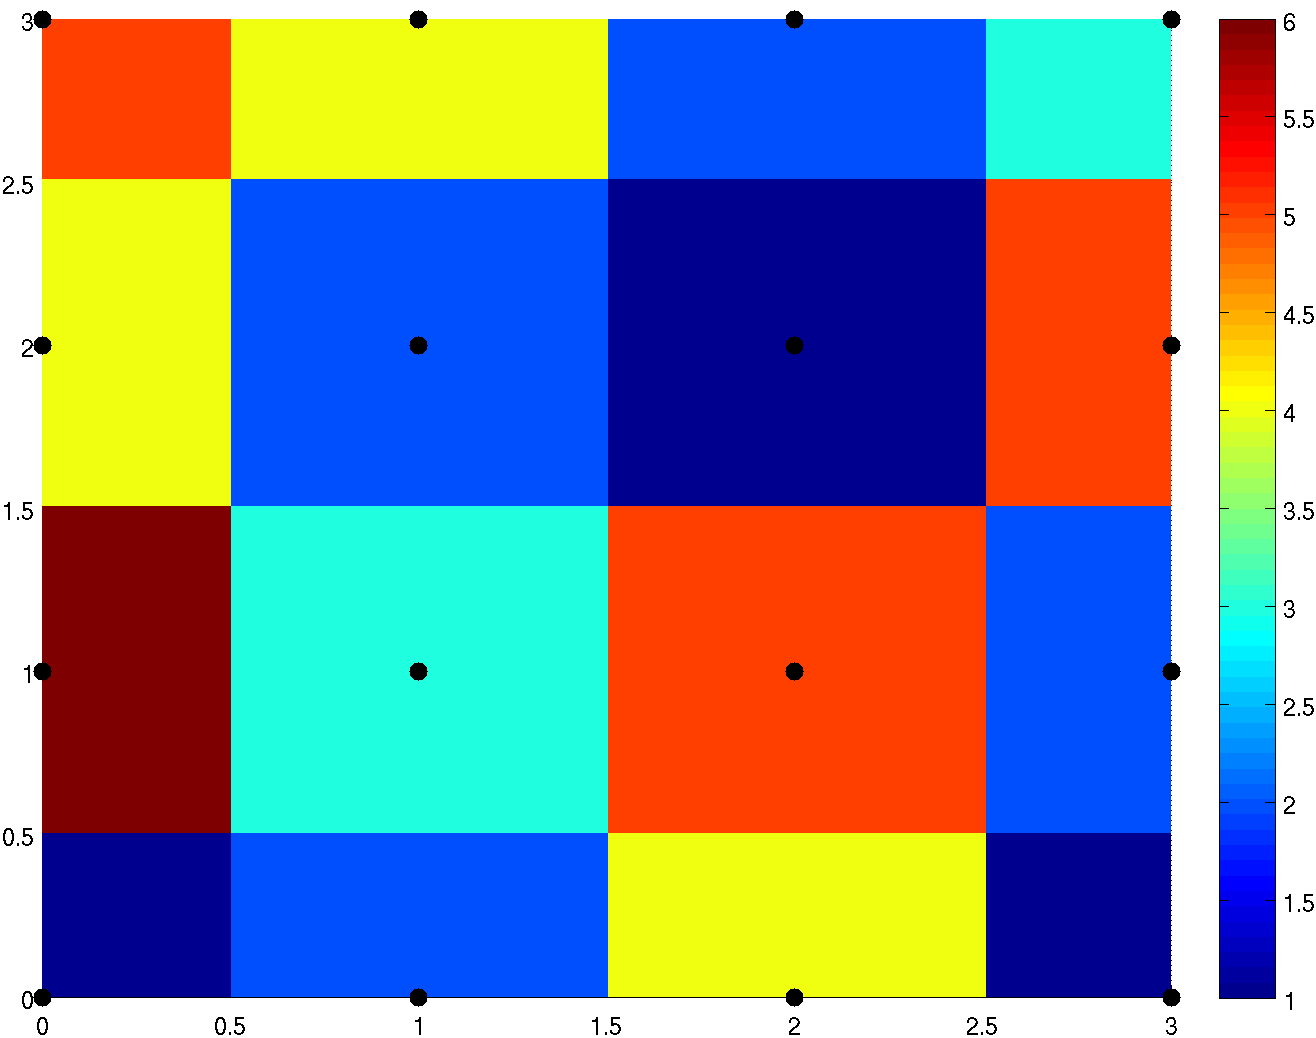
\includegraphics[width=\columnwidth]{Nearest2DInterpolExample.png}
    \column{0.33\textwidth}
      \centering
      \lstinline$'linear'$
      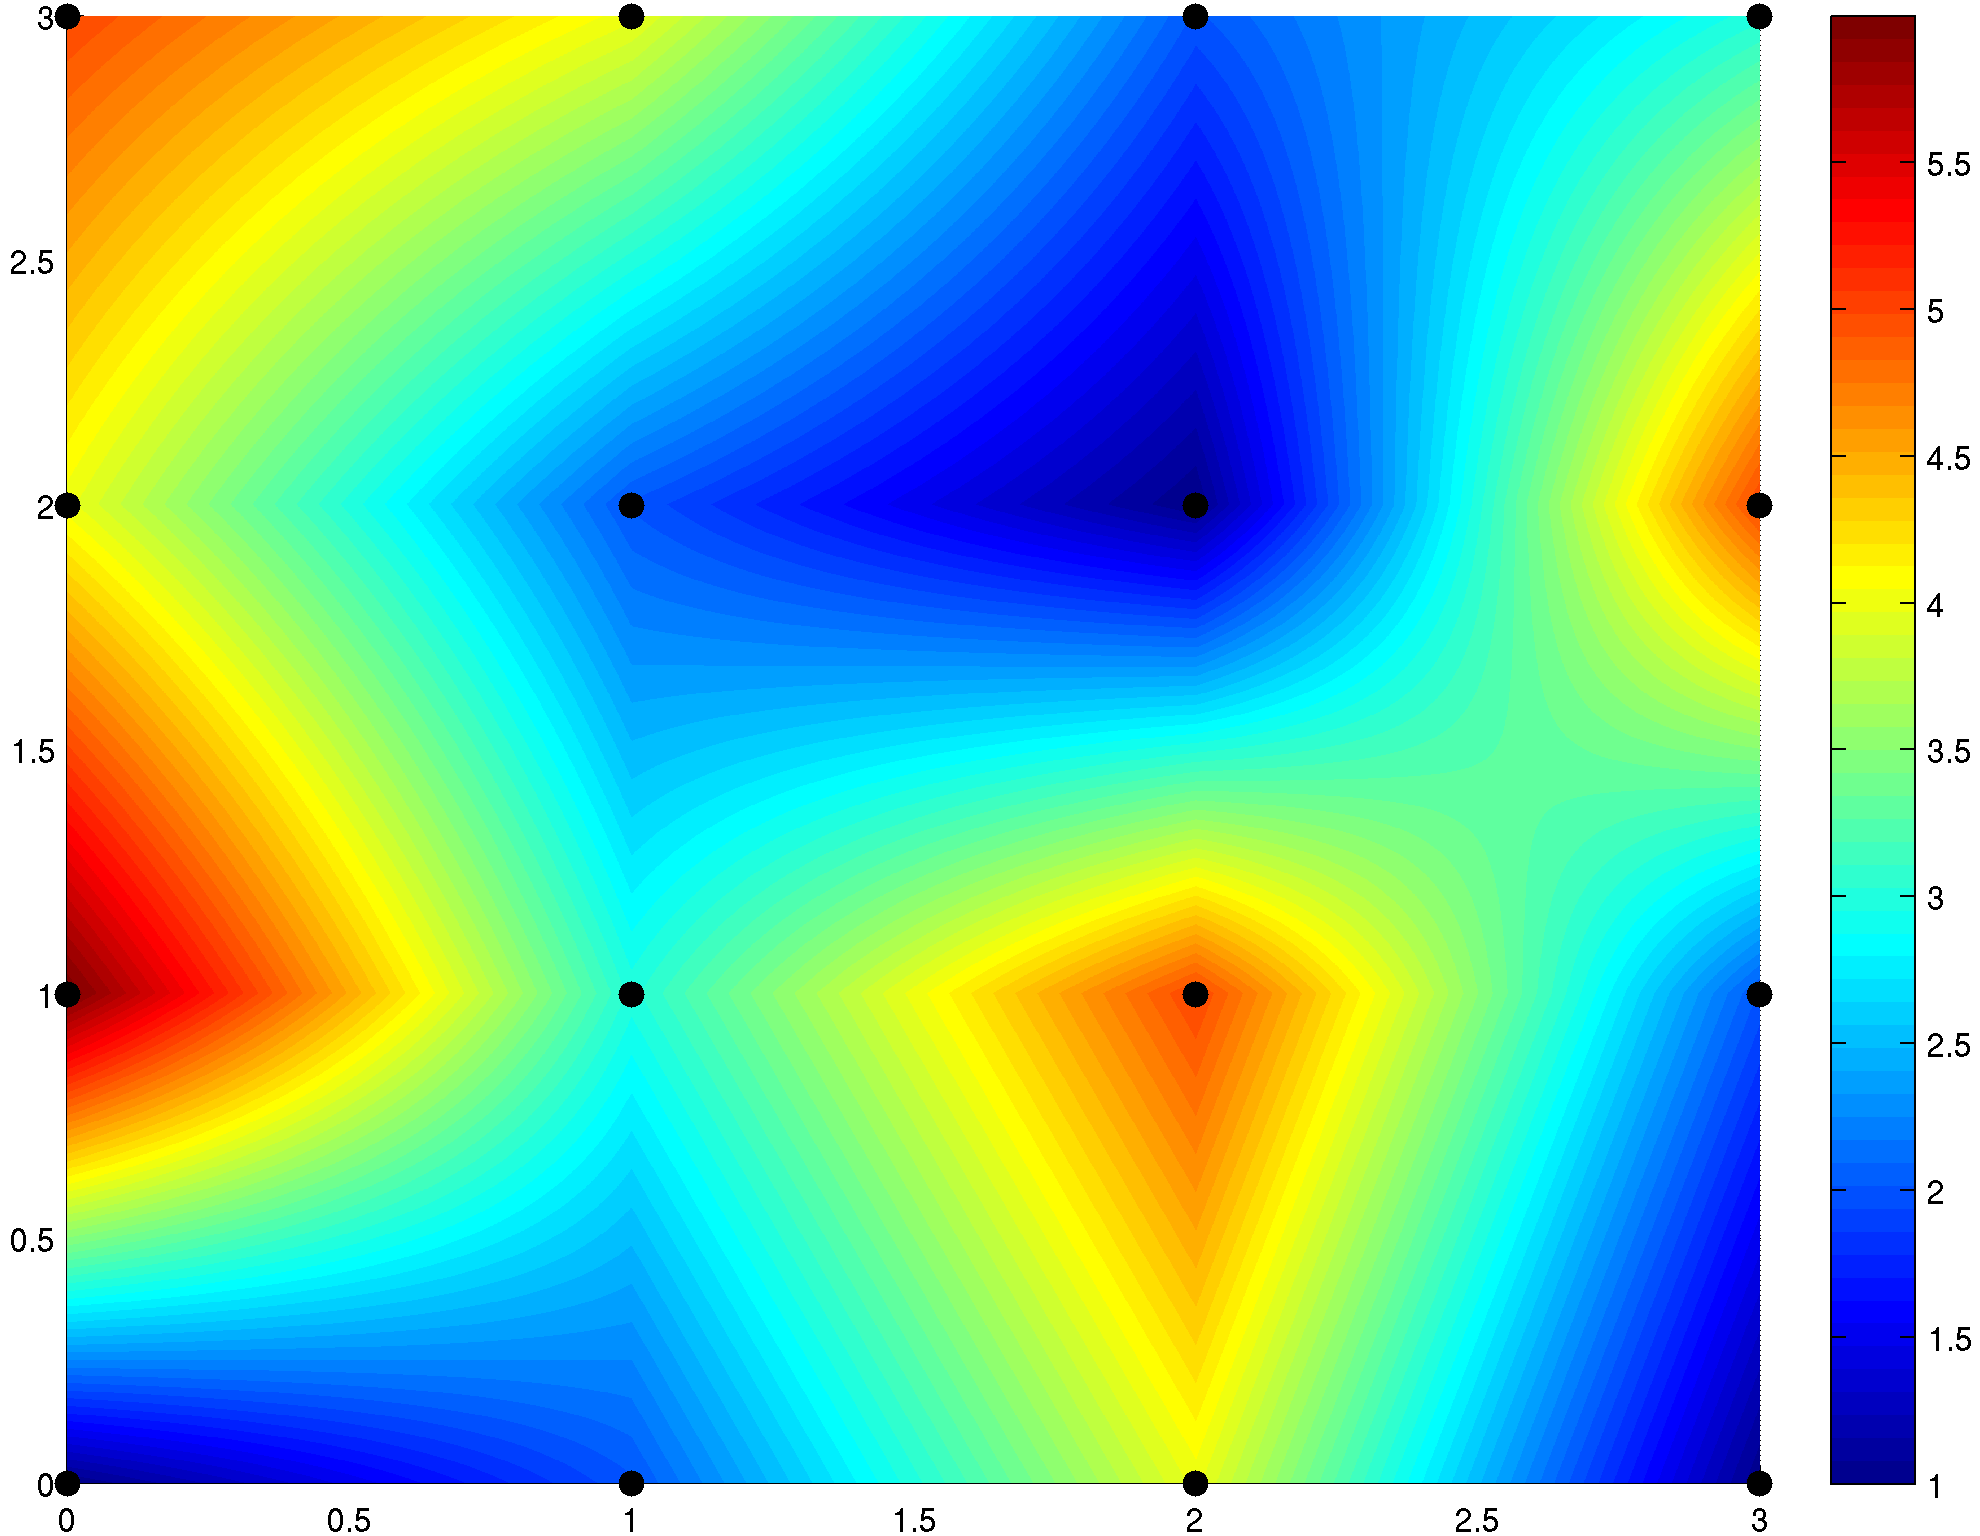
\includegraphics[width=\columnwidth]{BilinearInterpolExample.png}
    \column{0.33\textwidth}
      \centering
      \lstinline$'cubic'$
      \includegraphics[width=\columnwidth]{BicubicInterpolationExample.png}
  \end{columns}
  \vskip1em
  \begin{itemize}
    \item Similar to 1D linear interpolation, the derivatives are discontinuous on the grid nodes.
    \item Also consider tri-linear interpolation (for 3D fields) with \lstinline$scipy.interpolate.LinearNDInterpolator$, or bicubic interpolation (2D, but third order) with \lstinline$scipy.interpolate.interp2d$.
  \end{itemize}
\end{frame}


\begin{frame}
  \frametitle{A practical example}
  Field interpolation is used in e.g. CFD simulations, e.g. a fluidized bed simulation using a \emph{discrete particle model}, where particles are found in between the grid nodes used for velocity computation.\\
  \centering\includegraphics[width=0.4\textwidth]{fluidbed}
\end{frame}

\section{Polynomial}
\subsection*{}
\againframe<2>{contents_interpolation}
\begin{frame}
  \frametitle{Polynomial interpolation}
  The examples that we have seen, are simplified forms of \emph{Newton polynomials}. We can interpolate our data with a polynomial of degree $n$:
  
  \vskip2em
  \[
    p_n(x) = a_n x^n + a_{n-1}x^{n-1} + \ldots + a_2x^2 + a_1 x + a_0
  \]

\end{frame}

\begin{frame}[fragile]
  \frametitle{Polynomial interpolation via Vandermonde matrix}
  \footnotesize\selectfont
  \rowcolors[]{50}{white}{white}
  Consider the data points $(x_1,y_1),\, (x_2,y_2),\, \ldots,\,(x_m,y_m)$, the Vandermonde matrix $V$, coefficient vector $a$ and function value vector $y$: \vskip1em
  $V_{m,n} =
 \begin{pmatrix}
  x_1^0 & x_1^1 & x_1^2 & \cdots & x_1^{n-1} \\
  x_2^0 & x_2^1 & x_2^2 & \cdots & x_2^{n-1} \\
  \vdots  & \vdots & \vdots & \ddots & \vdots  \\
  x_m^0 & x_m^1 & x_m^2 & \cdots & x_m^{n-1}
 \end{pmatrix} \quad  
 a=
 \begin{pmatrix}
   a_0 \\
   a_1 \\
   \vdots\\
   a_{n-1}
 \end{pmatrix} \quad
 y=
 \begin{pmatrix}
   y_1 \\
   y_2 \\
   \vdots\\
   y_m
 \end{pmatrix}
$\vskip1em
The coefficients of a polynomial through the data points can be obtained by solving the linear system $Va=y$.
\pause
\begin{columns}
  \column{0.5\textwidth}
    \begin{lstlisting}[language=Python]
import numpy as np
x = np.array([0, 1, 2])
y = np.array([1.0000, 3.6667, 2.6667])
V = np.vander(x, increasing=True)
a = np.linalg.solve(V, y)
print(a)
# Output
# [-1.8333, 4.5000, 1.0000]
    \end{lstlisting}
  \column{0.5\textwidth}
  \pause
  So we found the equation:
  \[
    p_2(x) = -1.8333 x^2 + 4.5x - 1
  \]
  \pause
  \tikz{\node[emphblock,text width=\columnwidth] {These Vandermonde-systems are often \emph{ill-conditioned}, so we need another, more stable, method!
};}
\end{columns}
\end{frame}


\begin{frame}
  \frametitle{Construction of Newton polynomials}
  \footnotesize\selectfont
  Formally, the polynomials $p_n(x)$ are described using prefactors $f[x_0,\ldots,x_k]$ and polynomial terms $w_m(x)$:
  \[
    p_n(x) = \sum_{k=0}^n f[x_0,\ldots,x_k] w_k(x)
  \]
  \pause
  The polynomial terms are computed via:
  \begin{align*}
    &w_0(x) = 1, \ w_1(x)=(x-x_0), \ w_2(x)=(x-x_0)\cdot(x-x_1), \\
    &w_m(x)=(x-x_0)\cdot(x-x_1)\cdots(x-x_{m-1}) = w_{m-1}\cdot(x-x_{m-1})\\
    &w_m(x) = \prod_{j=0}^{m-1} (x-x_j), \qquad m=0,\ldots,n
  \end{align*}
  \pause
  The prefactors are \emph{forward divided differences}, which can be computed as:
    \[
      f[x_{x-k},\ldots,x_r] \equiv \frac{f[x_{r-k+1},\ldots,x_r]-f[x_{r-k},\ldots,x_{r-1}]}{x_r-x_{r-k}} 
    \]
\end{frame}

% 
%       \begin{align*}
% 	p_n(x)                &= \sum_{k=0}^n f[x_0,\ldots,x_k] w_k(x) \\
% 	w_m(x)                &= \prod_{j=0}^{m-1} (x-x_j) \\
% 	f[x_{x-k},\ldots,x_r] &\equiv \frac{f[x_{r-k+1},\ldots,x_r]-f[x_{r-k},\ldots,x_{r-1}]}{x_r-x_{r-k}} 
%       \end{align*}

\begin{frame}
  \frametitle{Construction of Newton polynomials: example}
  \footnotesize\selectfont
  \rowcolors[]{1}{maincolor!20}{maincolor!10}
  \begin{columns}[T]
    \begin{column}{0.2\textwidth}
    \centering Sample data
      \begin{longtable}{c|r}
	$x_k$ & $f_k$ \\ \hline
	$0$ & $1.00$ \\
	$1$ & $\frac{11}{3}=3.67$ \\
	$2$ & $\frac{8}{3}=2.67$ 
      \end{longtable}
    \end{column}
    \hfill
    \begin{column}{0.8\textwidth}
      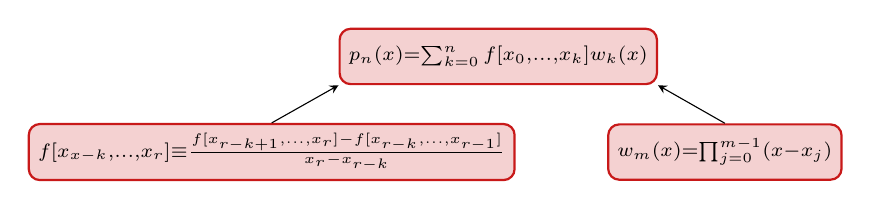
\begin{tikzpicture}[myNode/.style={rectangle,draw=maincolor,fill=maincolor!20,text centered,rounded corners,thick,minimum height=2em}]
	\node[myNode] (a) {${\scriptstyle p_n(x)= \sum_{k=0}^n f[x_0,\ldots,x_k] w_k(x)}$};
	\node[myNode,below left=1.2cm of a.south west,anchor=center] (c) {${\scriptstyle f[x_{x-k},\ldots,x_r] \equiv \frac{f[x_{r-k+1},\ldots,x_r]-f[x_{r-k},\ldots,x_{r-1}]}{x_r-x_{r-k}}}$};
	\node[myNode,below right=1.2cm of a.south east,anchor=center] (b) {${\scriptstyle w_m(x) = \prod_{j=0}^{m-1} (x-x_j)}$};
	\draw[->,>=stealth] (c.north) -> (a.south west);
	\draw[->,>=stealth] (b.north) -> (a.south east);
      \end{tikzpicture}
    \end{column}
  \end{columns}
    \onslide<2->{
      \begin{longtable}{c|ccc}
	$x_k$ & $f_k$ & & \\ \hline 
	\color<2>{tuered} $x_0$ & \color<2>{tuered} $f[x_0]=f_0$ & & \onslide<3->{\\
	\color<3>{tuered} $x_1$ & \color<3>{tuered} $f[x_1]=f_1$ & \color<3>{tuered} $f[x_0,x_1]=\frac{f_1-f_0}{x_1-x_0}$& \onslide<4->{\\
	\color<4>{tuered} $x_2$ & \color<4>{tuered} $f[x_2]=f_2$ & \color<4>{tuered} $f[x_1,x_2]=\frac{f_2-f_1}{x_2-x_1}$& \color<4>{tuered} $f[x_0,x_1,x_2] = \frac{f[x_1,x_2]-f[x_0,x_1]}{x_2-x_0}$ }}
      \end{longtable}}
  \onslide<2->{
    \begin{longtable}{c|lll}
      $x_k$ & $f_k$ & & \\ \hline
      \color<2>{tuered} $0$ & \color<2>{tuered} $1$ & & \onslide<3->{\\
      \color<3>{tuered} $1$ & \color<3>{tuered} $3.67$ & \color<3>{tuered} $\frac{\frac{11}{3}-1}{1-0}=\frac{8}{3}$& \onslide<4>{\\
      \color<4>{tuered} $2$ & \color<4>{tuered} $2.67$ & \color<4>{tuered} $\frac{\frac{8}{3}-\frac{11}{3}}{2-1}=\frac{-1}{1}=-1$& \color<4>{tuered} $\frac{(-1)-\frac{8}{3}}{2-0}=-\frac{11}{6}$ }}
    \end{longtable}
  }
\end{frame}

\begin{frame}
  \frametitle{Construction of Newton polynomials: example}
  \footnotesize\selectfont
  \rowcolors[]{1}{maincolor!20}{maincolor!10}
  \begin{columns}[T]
    \begin{column}{0.2\textwidth}
    \centering Sample data
      \begin{longtable}{c|r}
	$x_k$ & $f_k$ \\ \hline
	{\color<4->{tuedyellow}$0$} & $1.00$ \\
	{\color<4->{tuepurple}$1$} & $\frac{11}{3}=3.67$ \\
	$2$ & $\frac{8}{3}=2.67$ 
      \end{longtable}
    \end{column}
    \hfill
    \begin{column}{0.8\textwidth}
      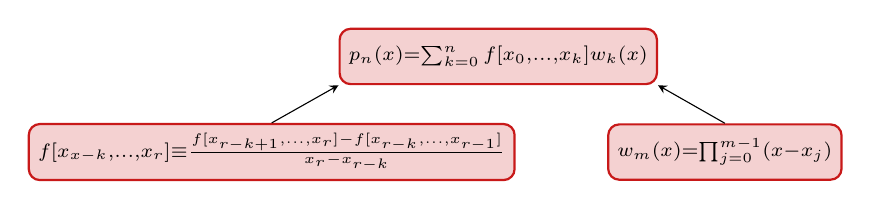
\begin{tikzpicture}[myNode/.style={rectangle,draw=maincolor,fill=maincolor!20,text centered,rounded corners,thick,minimum height=2em}]
	\node[myNode] (a) {${\scriptstyle p_n(x)= \sum_{k=0}^n f[x_0,\ldots,x_k] w_k(x)}$};
	\node[myNode,below left=1.2cm of a.south west,anchor=center] (c) {${\scriptstyle f[x_{x-k},\ldots,x_r] \equiv \frac{f[x_{r-k+1},\ldots,x_r]-f[x_{r-k},\ldots,x_{r-1}]}{x_r-x_{r-k}}}$};
	\node[myNode,below right=1.2cm of a.south east,anchor=center] (b) {${\scriptstyle w_m(x) = \prod_{j=0}^{m-1} (x-x_j)}$};
	\draw[->,>=stealth] (c.north) -> (a.south west);
	\draw[->,>=stealth] (b.north) -> (a.south east);
      \end{tikzpicture}
    \end{column}
  \end{columns}
  \pause
  \begin{longtable}{c|lll}
    $x_k$ & $f_k$                    & & \\ \hline
      $0$ & \color{tuered} $1$     & & \\
      $1$ &                  $3.67$ & $\frac{\frac{11}{3}-1}{1-0}=\color{tuered} \frac{8}{3}$& \\
      $2$ &                  $2.67$ & $\frac{\frac{8}{3}-\frac{11}{3}}{2-1}=\frac{-1}{1}=-1$   & $\frac{(-1)-\frac{8}{3}}{2-0}=\color{tuered}-\frac{11}{6}$ 
  \end{longtable}
  \onslide<3->{
    \begin{align*}
	p_2(x) &= {\color{tuered}1}\cdot w_m(0) + {\color{tuered}\frac{8}{3}}\cdot w_m(1) + \left({\color{tuered}-\frac{11}{6}}\right)\cdot w_m(2)   \\
	\onslide<4->{&= {\color{tuered}1}\cdot 1 + {\color{tuered}\frac{8}{3}}\cdot (x-{\color{tuedyellow}0}) + \left({\color{tuered}-\frac{11}{6}}\right)\cdot (x-{\color{tuedyellow}0})(x-{\color{tuepurple}1}) \onslide<5>{= \color{tuealert}-\frac{11}{6}x^2+4\frac{1}{2}x+1}}
    \end{align*}
  }
\end{frame}


\begin{frame}
  \frametitle{Construction of Newton polynomials: example}
  For each three points, a new polynomial interpolant can be derived:
  \begin{columns}
    \column{0.45\textwidth}
      \colorize<2>\color<2->{tuered} \[ p_2(x) = -\frac{11}{6}x^2+4\frac{1}{2}x+1 \]
      \colorize<3>\color<3->{tuelila}   \[ p_2(x) = 4-\frac{x^2}{3} \]
      \colorize<4>\color<4->{tuelblue}  \[ p_2(x) = \frac{7x^2}{6}-7\frac{1}{2}x+13 \]
      \colorize<5>\color<5->{tuedyellow} \[ p_2(x) = \frac{8}{3}x^2-18x+31 \]
      \colorize<6>\color<6>{tuedgreen} \[ f(x)=\frac{x^3}{2}-\frac{10x^2}{3}+\frac{11x}{2}+1 \]
    \column{0.55\textwidth}
    \centering
    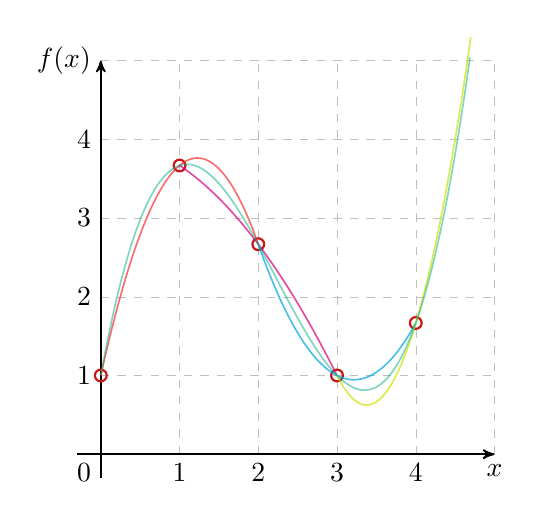
\begin{tikzpicture}[domain=-1:6]
        \draw[gridline,step=1] (0,0) grid (5,5);
  \coordinate (O) at (0,0);
  % Axes
  \draw[line,->] (-0.3,0) -- (5,0) coordinate[label = {below:$x$}] (xmax);
  \draw[line,->] (0,-0.3) -- (0,5) coordinate[label = {left:$f(x)$}] (ymax);
  
  % Labels
  \draw (0,0) node[below left]{$0$};
  \foreach \s in {1,...,4}
  {
    \draw (\s,0) node[below]{$\s$};
    \draw (0,\s) node[left]{$\s$};
    }
    
    % Title
    %       \draw (2.5,5) node[above]{$f(x)=\frac{x^3}{2}-\frac{10x^2}{3}+\frac{11x}{2}+1$};
    
    % Plots
    \node[interp] (x0) at (0,1) {};
    \node[interp] (x1) at (1,3.667) {};
    \node[interp] (x2) at (2,2.667) {};
    \node[interp] (x3) at (3,1) {};
    \node[interp] (x4) at (4,1.667) {};
    \node (bb) at (5,5.3) {};
%       \draw [graph,domain=0:4.69] plot (\x, {0.5*\x*\x*\x-(10/3)*\x*\x+5.5*\x+1});
%       \draw [graph,opacity=0.4,dashed,domain=-0.15:4.73] plot (\x, {0.5*\x*\x*\x-(10/3)*\x*\x+5.5*\x+1});


      % Polynomial interpolant
      \draw<2-> [graph,domain=0:2,draw=tuered,opacity=0.7] plot (\x, {-(11/6)*\x*\x+(4.5)*\x+1});
      \draw<3-> [graph,domain=1:3,draw,tuelila,opacity=0.7] plot (\x, {(-1/3)*\x*\x+4});
      \draw<4-> [graph,domain=2:4,draw=tuelblue,opacity=0.7] plot (\x, {(7/6)*\x*\x-7.5*\x + 13});
      \draw<5-> [graph,domain=3:4.7,draw=tuedyellow,opacity=0.7] plot (\x, {(8/3)*\x*\x-18*\x+31});
      \draw<6> [graph,domain=0:4.69,draw=tuedgreen,opacity=0.5] plot (\x, {0.5*\x*\x*\x-(10/3)*\x*\x+5.5*\x+1});
    \end{tikzpicture}
    % \onslide<6>{

    % }
    \vfill
  \end{columns}
\end{frame}

\begin{frame}[fragile]
  \frametitle{Polynomial fitting in Python: example}
  \rowcolors[]{1}{maincolor!20}{maincolor!10}
  \footnotesize\selectfont
     \begin{columns}
    \column{0.45\textwidth}
    Develop the {\color<5->{tuered}$p_2(x)$}, {\color<6->{tuedgreen}$p_3(x)$} and {\color<7>{tuelblue}$p_4(x)$} from the following data set (example data \lstinline$x2$ and \lstinline$y2$): 
    \vspace*{-1ex}
    \begin{center}
      \begin{tabular}{c|r}
	$x_k$ & $y_k$ \\ \hline
	$-1.0$ & $2.8677$ \\
	$-0.5$ & $7.7530$ \\
	$0.0$ & $22.0000$  \\
	$0.5$ & $65.7863$ \\
	$1.0$ & $208.6744$  \\ \hline
      \end{tabular}
    \end{center}
    \column{0.55\textwidth}
    \centering
    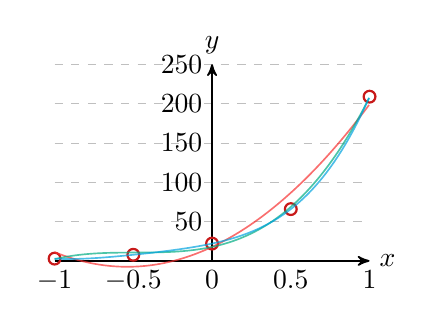
\begin{tikzpicture}[domain=-1:1,xscale=2,yscale=0.01]
      \draw[gridline,step=50] (-1,0) grid (1,250);
      \coordinate (O) at (0,0);
      % Axes
      \draw[line,->] (-1,0) -- (1,0) coordinate[label = {right:$x$}] (xmax);
      \draw[line,->] (0,0) -- (0,250) coordinate[label = {above:$y$}] (ymax);

      % Labels
%       \draw (0,0) node[below left]{$0$};
      \foreach \s in {-1,-0.5,...,1}
      {
        \draw (\s,0) node[below]{$\s$};
      }
      \foreach \s in {50,100,...,250}
      {
        \draw (0,\s) node[left]{$\s$};
      }

      % Title
%       \draw (2.5,5) node[above]{$f(x)=\frac{x^3}{2}-\frac{10x^2}{3}+\frac{11x}{2}+1$};

      % Plots
       \node[interp] (x0) at (-1,2.8677) {};
       \node[interp] (x1) at (-0.5,7.753) {};
       \node[interp] (x2) at ( 0.0,22.00) {};
       \node[interp] (x3) at ( 0.5,65.7863) {};
       \node[interp] (x4) at ( 1.0,208.6744) {};
       
       \draw<5-> [graph,draw=tuered,opacity=0.7,domain=-1:1] plot (\x, {87.2986*\x*\x+93.9293*\x+17.7670});
       \draw<6-> [graph,draw=tuedgreen,opacity=0.7,domain=-1:1] plot (\x, {59.8267*\x*\x*\x+87.2986*\x*\x+43.0766*\x+17.7670});
       \draw<7> [graph,draw=tuelblue,opacity=0.7,domain=-1:1] plot (\x, {32.9234*\x*\x*\x*\x+59.8267*\x*\x*\x+50.8477*\x*\x+43.0766*\x+22.0000});
    \end{tikzpicture}
  \end{columns}
  \pause \vskip1ex
  We use the built-in \lstinline$np.polyfit(x,y,n)$ and \lstinline$np.polyval(p,x)$ functions: \pause
  \begin{columns}
    \column{0.5\textwidth}
  \begin{lstlisting}[language=Python,basicstyle=\tiny]
import numpy as np, matplotlib.pyplot as plt
x_cont = np.linspace(-1, 1, 1001)
p2 = np.polyfit(x2, y2, 2)
p3 = np.polyfit(x2, y2, 3)
p4 = np.polyfit(x2, y2, 4)

y_cont2 = np.polyval(p2, x_cont)
y_cont3 = np.polyval(p3, x_cont)
y_cont4 = np.polyval(p4, x_cont)

plt.plot(x2, y2, 'o', label='Data points')
plt.plot(x_cont, y_cont2, label='Degree 2')
plt.plot(x_cont, y_cont3, label='Degree 3')
plt.plot(x_cont, y_cont4, label='Degree 4')
plt.legend()
plt.show()
   \end{lstlisting}
   \column{0.3\textwidth}
  \end{columns}
\end{frame}


\begin{frame}[fragile]
  \frametitle{Exercise}
  \rowcolors[]{1}{maincolor!20}{maincolor!10}
  \footnotesize\selectfont
  Develop the {\color<4->{tuered}$p_4(x)$} and {\color<5>{tueorange}$p_{10}(x)$} interpolants from the following data sets: 
  \vspace*{1em}
\[
f(x)=\frac{1}{x^2+\frac{1}{25}} \qquad x \in [-1,1]
\]
     \begin{lstlisting}[language=Python]
import numpy as np
x3a, x3b = np.linspace(-1, 1, 5), np.linspace(-1, 1, 11)
y3a, y3b = 1 / (x3a**2 + 1/25), 1 / (x3b**2 + 1/25)
     \end{lstlisting}
    \begin{tikzpicture}[domain=-1:1,xscale=2,yscale=0.1]
      % (the tikzpicture content remains unchanged)
    \end{tikzpicture}
  \vspace*{-1ex}
  \begin{lstlisting}[language=Python, basicstyle=\scriptsize]
import matplotlib.pyplot as plt
x_cont = np.linspace(-1, 1, 1001)
p4, p10 = np.polyfit(x3a, y3a, 4), np.polyfit(x3b, y3b, 10)
y_cont4, y_cont10 = np.polyval(p4, x_cont), np.polyval(p10, x_cont)

plt.plot(x_cont, 1 / (x_cont**2 + 1/25), label='f(x)')
plt.scatter(x3a, y3a, marker='o', label='p4 data')
plt.scatter(x3b, y3b, marker='x', label='p10 data')
plt.plot(x_cont, y_cont4, label='p4(x)')
plt.plot(x_cont, y_cont10, label='p10(x)')
plt.legend()
plt.show()
  \end{lstlisting}
\end{frame}


\begin{frame}
  \frametitle{Final thoughts on polynomial interpolation}
%   \pause
  \begin{itemize}
    \colorize<1> \item An polynomial interpolant of order $n$ requires $n+1$ data points
    \begin{itemize}
     \colorize<1>  \item More data points: interpolant does \emph{not always} cross the points
     \colorize<1>  \item Fewer data points: interpolant is not unique
    \end{itemize}
    \colorize<2> \item Higher-degree polynomials at equidistant points may cause strong oscillatory behaviour (Runge's phenomenon)
    \begin{itemize}
      \colorize<2> \item Mitigation of the problem on Chebyshev (i.e. non uniform grid)...
      \colorize<2> \item ... or by performing piecewise interpolation (next topic)
    \end{itemize}
    \colorize<3> \item Python functions \lstinline$np.polyfit(x,y,n)$ and \lstinline$np.polyval(p,x_new)$ were demonstrated.
  \end{itemize}
\end{frame}

\section{Splines}
\subsection*{}
\againframe<2>{contents_interpolation}
\begin{frame}
  \frametitle{Spline interpolation}
  A spline is a numerical function that represents a {\color{tuealert}smooth}, {\color{tuealert}higher order}, {\color{tuealert}piecewise polynomial} interpolants of a data set.
  \pause
  \begin{itemize}
    \colorize<2> \item Smooth: the interpolant is continuous in the first and second derivatives 
    \colorize<3> \item Higher order: The most common type of splines uses third-order polynomials (cubic splines)
    \colorize<4> \item Piecewise polynomial: The interpolant is constructed between each two consecutive tabulated points
  \end{itemize}
\end{frame}

\begin{frame}
  \frametitle{Splines: comparison to other interpolation techniques}
  \footnotesize\selectfont
  Interpolation of $\displaystyle f(x) = \frac{\sin x}{1+x^2}$
  \begin{center}
    \begin{tikzpicture}
%       \tikzset{at/.style=}
      \begin{axis}[every axis/.append style={font=\tiny},
	width=\textwidth, height=8cm,     % size of the image
	grid = major,
	grid style={dashed, gray!30},
	%xmode=log,log basis x=10,
	%ymode=log,log basis y=10,
	xmin=-4,     % start the diagram at this x-coordinate
	xmax=4,    % end   the diagram at this x-coordinate
	ymin=-0.7,     % start the diagram at this y-coordinate
	ymax=0.7,   % end   the diagram at this y-coordinate
	xtick={-3,-2,...,3},
	xticklabels={ ,-2,-1,...,3}, 
	/pgfplots/ytick={-0.5,0,0.5},
	axis background/.style={fill=white},
	axis x line=middle,
	axis y line=middle,
	ylabel=$f(x)$,
	xlabel=$x$,
	tick align=outside,
	legend style={draw=none,fill=none,font=\tiny,at={(0.5,1.0)},anchor=south},
% 	legend style={pos=outside}
	legend columns=5
	]

	% Actual equation
	\only<1>{\addplot[graph,domain=-4:4] {sin(deg(x))/(1+x*x)};}
	\only<2->{\addplot[graph,domain=-4:4,opacity=0.3] {sin(deg(x))/(1+x*x)};}
	\addlegendentry{Function}
	% Nodes
	\only<2->{\addplot[samples=9,nodes near coords={\color{black}$f_\coordindex$},mark=*,mark options={fill=white,color=tuered},only marks,domain=-4:4] {sin(deg(x))/(1+x*x)};}
	\addlegendentry{Nodes}
	
	% Linear
	\only<3>{\addplot[graph,sharp plot,samples=9,domain=-4:4,draw=tueblue] {sin(deg(x))/(1+x*x)};}
	\only<4-5>{\addplot[graph,sharp plot,samples=9,domain=-4:4,draw=tueblue,opacity=0.3] {sin(deg(x))/(1+x*x)};}
	\addlegendentry{Linear}
	% Polynomial
	\only<4>{\addplot[graph,domain=-4:4,draw=tuegreen] {-6.891773605597105e-04*x^7+2.123474572587917e-02*x^5-2.016362539647688e-01*x^3+6.018261780033977e-01*x};}
	\only<5>{\addplot[graph,domain=-4:4,draw=tuegreen,opacity=0.3] {-6.891773605597105e-04*x^7+2.123474572587917e-02*x^5-2.016362539647688e-01*x^3+6.018261780033977e-01*x};}
	\addlegendentry{Polynomial}
	\only<5>{\addplot[graph,draw=tuefuchsia] table [id=spline]{data/spline_data.txt};}
	\addlegendentry{Spline}
      \end{axis} 
    \end{tikzpicture}
  \end{center}
\end{frame}

\begin{frame}[fragile]
  \frametitle{Spline interpolation in Python}
  We can generate a random data set, and interpolate using \lstinline$scipy.interpolate.interp1d$: 
  \vskip0.5ex \pause
  \begin{lstlisting}[language=Python,basicstyle=\tiny]
import numpy as np
import matplotlib.pyplot as plt
from scipy.interpolate import interp1d
# Generate random data set
x = np.arange(0, 26)
y = np.random.rand(len(x))
# Interpolant on a fine mesh
xc = np.linspace(0, 25, 1001)
yc = interp1d(x, y, kind='cubic')(xc)
# Plot the data
plt.plot(x, y, 'o')
plt.plot(xc, yc, '-r')
  \end{lstlisting} \vskip1ex
        \begin{tikzpicture}
      \begin{axis}[every axis/.append style={font=\footnotesize},
    width=\columnwidth, height=5cm,     % size of the image
    grid = major,
    grid style={dashed, gray!30},
    xmin=0,     % start the diagram at this x-coordinate
    xmax=26,    % end   the diagram at this x-coordinate
    ymin=0,     % start the diagram at this y-coordinate
    ymax=1.3,   % end   the diagram at this y-coordinate
    xtick={0,-2,...,25},
    /pgfplots/ytick={0,0.5,1},
    axis background/.style={fill=white},
    axis x line=middle,
    axis y line=middle,
    ylabel=$f(x)$,
    xlabel=$x$,
    tick align=outside,
    ]

      \addplot[interp,draw=none,mark=*] table [id=spline]{data/spline_data1.txt};
      \addplot[graph] table [id=spline]{data/spline_data2.txt};
    \end{axis} 
  \end{tikzpicture}
\end{frame}

\begin{frame}
  \frametitle{Summary}
  \begin{itemize}
    \item Interpolation is used to obtain data between existing data points
    \begin{itemize}
      \item (Bi-)Linear, polynomial and spline interpolation methods
      \item Construction of Newton polynomials
      \item Oscillations of high-order polynomials
    \end{itemize}
    \item Legendre polynomials: alternative way of performing the polynomial interpolation (not discussed here)
  \end{itemize}
\end{frame}

\section{Tutorials}
\subsection*{Interpolation tutorials}
\begin{frame}[fragile]
  \frametitle{Interpolation tutorials}
  \begin{enumerate}
    \item In Python, generate the data:
    \begin{lstlisting}
x = np.arange(-4, 6, 1)
y = [0, 0, 0, 1, 1, 1, 0, 0, 0, 0]
    \end{lstlisting}
    Interpolate the data using polynomial interpolation (which order do you use?) and a spline. Plot the results together with the original data in a graph.
    \item Do the same exercise for the following data. Can you explain your observations?
    \begin{lstlisting}
t = [0, 0.1, 0.499, 0.5, 0.6, 1.0, 1.4, 1.5, 1.899, 1.9, 2.0]
y = [0, 0.06, 0.17, 0.19, 0.21, 0.26, 0.29, 0.29, 0.30, 0.31, 0.31]
    \end{lstlisting}
  \end{enumerate}
\end{frame}


\title{Numerical integration}
\subtitle{}
\lecture{integration}{integration}
\section{Introduction}
\subsection*{General}
\begin{frame}[label=contents_integration]
  \frametitle{Today's outline}
  \mode<beamer>{
    \only<1>{\tableofcontents}
  }
  \only<2>{\tableofcontents[currentsection,currentsubsection]}
\end{frame}

\frame{
  \frametitle{What is numerical integration?}
  To determine the integral $I(x)$ of an integrand $f(x)$, which can be used to compute the area underneath the integrand between $x=a$ and $x=b$.
  \[
    I(x) = \int_a^b f(x)dx
  \]
  \pause
  Today we will outline different numerical integration methods.
  \vskip2em
  \begin{itemize}
    \item Riemann integrals
    \item Trapezoidal rule
    \item Simpson's rule
  \end{itemize}
}
\begin{frame}
  \frametitle{Why do chemical engineers need integration?}
  \begin{itemize}
    \colorize<1> \item Obtaining the cumulative particle size distribution from a particle size distribution
    \colorize<2> \item The concentration outflow over time may be integrated to yield the residence time distribution
    \colorize<3> \item Integration of a varying product outflow yields the total product outflow
    \colorize<4> \item Quantitative analysis of mixture components via e.g. GC/MS
    \colorize<5> \item Not all function have an explicit antiderivative, e.g. $\int e^{x^2} dx$ or $\int \frac{1}{\ln x}dx$
  \end{itemize}
\end{frame}

\section{Riemann integrals}
\againframe<2>{contents_integration}
\begin{frame}
  \frametitle{Riemann integrals}
  \footnotesize\selectfont
  \tikz{\node[emphblock,text width=\textwidth] {Basic idea: Subdivide the interval $[a,b]$ into $n$ subintervals of equal length $\Delta x = \frac{b-a}{n}$ and use the sum of area to approximate the integral.};}
  \pause
  \begin{columns}[T]
 \column{0.33\textwidth}
    \begin{center}
      Left endpoint rule \vskip1em
      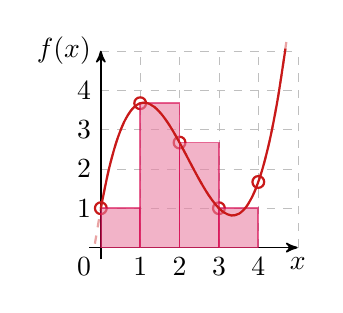
\begin{tikzpicture}[scale=0.5]
          \draw[gridline,step=1] (0,0) grid (5,5);
  \coordinate (O) at (0,0);
  % Axes
  \draw[line,->] (-0.3,0) -- (5,0) coordinate[label = {below:$x$}] (xmax);
  \draw[line,->] (0,-0.3) -- (0,5) coordinate[label = {left:$f(x)$}] (ymax);
  
  % Labels
  \draw (0,0) node[below left]{$0$};
  \foreach \s in {1,...,4}
  {
    \draw (\s,0) node[below]{$\s$};
    \draw (0,\s) node[left]{$\s$};
    }
    
    % Title
    %       \draw (2.5,5) node[above]{$f(x)=\frac{x^3}{2}-\frac{10x^2}{3}+\frac{11x}{2}+1$};
    
    % Plots
    \node[interp] (x0) at (0,1) {};
    \node[interp] (x1) at (1,3.667) {};
    \node[interp] (x2) at (2,2.667) {};
    \node[interp] (x3) at (3,1) {};
    \node[interp] (x4) at (4,1.667) {};
    \node (bb) at (5,5.3) {};
%       \draw [graph,domain=0:4.69] plot (\x, {0.5*\x*\x*\x-(10/3)*\x*\x+5.5*\x+1});
%       \draw [graph,opacity=0.4,dashed,domain=-0.15:4.73] plot (\x, {0.5*\x*\x*\x-(10/3)*\x*\x+5.5*\x+1});

        
        \draw [intblock] (1,0) rectangle (x0);
        \draw [intblock] (2,0) rectangle (x1);
        \draw [intblock] (3,0) rectangle (x2);
        \draw [intblock] (4,0) rectangle (x3);
        
        \draw [interp,smooth,domain=0:4.69] plot (\x, {0.5*\x*\x*\x-(10/3)*\x*\x+5.5*\x+1});
        \draw [interp,smooth,opacity=0.4,dashed,domain=-0.15:4.73] plot (\x, {0.5*\x*\x*\x-(10/3)*\x*\x+5.5*\x+1});
      \end{tikzpicture}
      \[
        L_n = \sum_{i=1}^n f(x_{i-1})\Delta x_i
      \]
    \end{center}
    \pause
    \column{0.33\textwidth}
    \begin{center}
      Right endpoint rule \vskip1em
      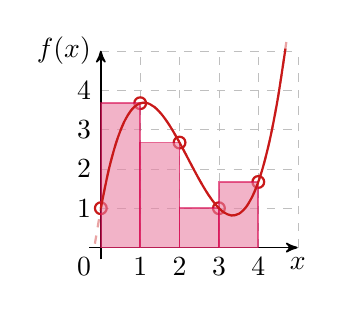
\begin{tikzpicture}[scale=0.5]
          \draw[gridline,step=1] (0,0) grid (5,5);
  \coordinate (O) at (0,0);
  % Axes
  \draw[line,->] (-0.3,0) -- (5,0) coordinate[label = {below:$x$}] (xmax);
  \draw[line,->] (0,-0.3) -- (0,5) coordinate[label = {left:$f(x)$}] (ymax);
  
  % Labels
  \draw (0,0) node[below left]{$0$};
  \foreach \s in {1,...,4}
  {
    \draw (\s,0) node[below]{$\s$};
    \draw (0,\s) node[left]{$\s$};
    }
    
    % Title
    %       \draw (2.5,5) node[above]{$f(x)=\frac{x^3}{2}-\frac{10x^2}{3}+\frac{11x}{2}+1$};
    
    % Plots
    \node[interp] (x0) at (0,1) {};
    \node[interp] (x1) at (1,3.667) {};
    \node[interp] (x2) at (2,2.667) {};
    \node[interp] (x3) at (3,1) {};
    \node[interp] (x4) at (4,1.667) {};
    \node (bb) at (5,5.3) {};
%       \draw [graph,domain=0:4.69] plot (\x, {0.5*\x*\x*\x-(10/3)*\x*\x+5.5*\x+1});
%       \draw [graph,opacity=0.4,dashed,domain=-0.15:4.73] plot (\x, {0.5*\x*\x*\x-(10/3)*\x*\x+5.5*\x+1});

        \draw [intblock] (0,0) rectangle (x1);
        \draw [intblock] (1,0) rectangle (x2);
        \draw [intblock] (2,0) rectangle (x3);
        \draw [intblock] (3,0) rectangle (x4);
        
        \draw [interp,smooth,domain=0:4.69] plot (\x, {0.5*\x*\x*\x-(10/3)*\x*\x+5.5*\x+1});
        \draw [interp,smooth,opacity=0.4,dashed,domain=-0.15:4.73] plot (\x, {0.5*\x*\x*\x-(10/3)*\x*\x+5.5*\x+1});
      \end{tikzpicture}
      \[
        R_n = \sum_{i=1}^n f(x_i)\Delta x_i
      \]

    \end{center}
    \pause
    \column{0.33\textwidth}
      \begin{center}
        Midpoint rule \vskip1em
        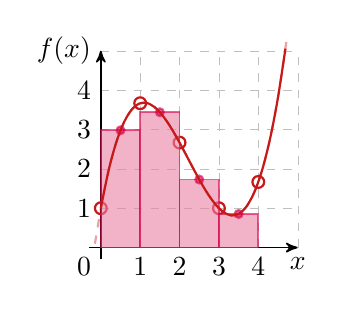
\begin{tikzpicture}[scale=0.5]
            \draw[gridline,step=1] (0,0) grid (5,5);
  \coordinate (O) at (0,0);
  % Axes
  \draw[line,->] (-0.3,0) -- (5,0) coordinate[label = {below:$x$}] (xmax);
  \draw[line,->] (0,-0.3) -- (0,5) coordinate[label = {left:$f(x)$}] (ymax);
  
  % Labels
  \draw (0,0) node[below left]{$0$};
  \foreach \s in {1,...,4}
  {
    \draw (\s,0) node[below]{$\s$};
    \draw (0,\s) node[left]{$\s$};
    }
    
    % Title
    %       \draw (2.5,5) node[above]{$f(x)=\frac{x^3}{2}-\frac{10x^2}{3}+\frac{11x}{2}+1$};
    
    % Plots
    \node[interp] (x0) at (0,1) {};
    \node[interp] (x1) at (1,3.667) {};
    \node[interp] (x2) at (2,2.667) {};
    \node[interp] (x3) at (3,1) {};
    \node[interp] (x4) at (4,1.667) {};
    \node (bb) at (5,5.3) {};
%       \draw [graph,domain=0:4.69] plot (\x, {0.5*\x*\x*\x-(10/3)*\x*\x+5.5*\x+1});
%       \draw [graph,opacity=0.4,dashed,domain=-0.15:4.73] plot (\x, {0.5*\x*\x*\x-(10/3)*\x*\x+5.5*\x+1});

          
          \draw [intblock] (0,0) rectangle (1,2.9792);
          \node [intdot] at (0.5, 2.9792) {};
          \draw [intblock] (1,0) rectangle (2,3.4375);
          \node [intdot] at (1.5, 3.4375) {};
          \draw [intblock] (2,0) rectangle (3,1.7292);
          \node [intdot] at (2.5, 1.7292) {};
          \draw [intblock] (3,0) rectangle (4,0.8542);
          \node [intdot] at (3.5, 0.8542) {};
          
          \draw [interp,smooth,domain=0:4.69] plot (\x, {0.5*\x*\x*\x-(10/3)*\x*\x+5.5*\x+1});
          \draw [interp,smooth,opacity=0.4,dashed,domain=-0.15:4.73] plot (\x, {0.5*\x*\x*\x-(10/3)*\x*\x+5.5*\x+1});
        \end{tikzpicture}
        \[
          M_n = \sum_{i=1}^n f(\bar{x}_i)\Delta x_i
        \]
        with $\bar{x}_i = \frac{x_{i-1}+x_i}{2}$
      \end{center}
  \end{columns}
\end{frame}

\begin{frame}
  \frametitle{Errors in Riemann integrals}
  We define the exact integral as $ I = \int_a^b f(x)dx$, and $L_n$, $R_n$ and $M_n$ represent the left, right and midpoint rule approximations of $I$ based on $n$ intervals.
  \vskip1em \pause
  Writing $f^{(k)}_\text{max}$ for the maximum value of the $k$-th derivative, the upper-bounds of the errors by Riemann integrals are: \vskip1em
  \begin{itemize}
    \colorize<2> \item $\displaystyle \abs{I - L_n} \leq \frac{f^{(1)}_\text{max} (b - a)^2}{2n}$
    \colorize<3> \item $\displaystyle \abs{I - R_n} \leq \frac{f^{(1)}_\text{max} (b - a)^2}{2n}$
    \colorize<4> \item $\displaystyle \abs{I - M_n} \leq \frac{f^{(2)}_\text{max} (b - a)^3}{24n^2}$
  \end{itemize}
  \vskip1em
  \onslide<5>{%
Note that while $\abs{I - L_n}$ and $\abs{I - R_n}$ give the same \emph{upper-bounds} of the error, this does not mean the same error. Rather, the error is of opposite sign!}
\end{frame}

\section{Trapezoid rule}
\againframe<2>{contents_integration}
\begin{frame}
  \frametitle{Trapezoid rule}
  \footnotesize\selectfont
  Since the sign of the approximation error of the left and right endpoint rules is opposite, we can take the average of these approximations:
  \[
    T_n = \frac{L_n + R_n}{2}
  \]
  \pause
  \begin{columns}
\column{0.5\textwidth}
  The total area is obtained by geometric reconstruction of trapezoids:
  \[
    T_n = \sum_{i=1}^n \frac{f(x_{i+1})+f(x_i)}{2}\Delta x_i
  \]
\onslide<3>{%
Note that this can be rewritten for equidistant intervals:
\begin{equation*}
  T_n = \frac{b-a}{2n} \left( f(x_0) + 2f(x_1) + \ldots + 2f(x_{n-1}) + f(x_n) \right)
\end{equation*}}
\column{0.5\textwidth}
   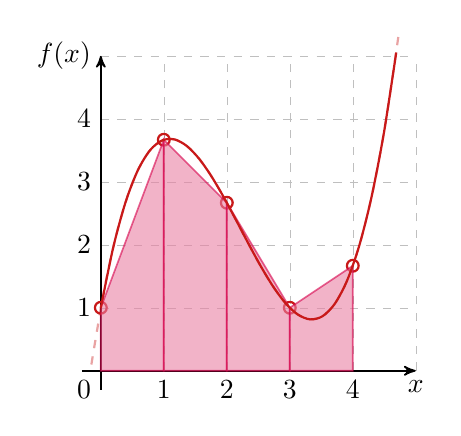
\begin{tikzpicture}[scale=0.8]
          \draw[gridline,step=1] (0,0) grid (5,5);
  \coordinate (O) at (0,0);
  % Axes
  \draw[line,->] (-0.3,0) -- (5,0) coordinate[label = {below:$x$}] (xmax);
  \draw[line,->] (0,-0.3) -- (0,5) coordinate[label = {left:$f(x)$}] (ymax);
  
  % Labels
  \draw (0,0) node[below left]{$0$};
  \foreach \s in {1,...,4}
  {
    \draw (\s,0) node[below]{$\s$};
    \draw (0,\s) node[left]{$\s$};
    }
    
    % Title
    %       \draw (2.5,5) node[above]{$f(x)=\frac{x^3}{2}-\frac{10x^2}{3}+\frac{11x}{2}+1$};
    
    % Plots
    \node[interp] (x0) at (0,1) {};
    \node[interp] (x1) at (1,3.667) {};
    \node[interp] (x2) at (2,2.667) {};
    \node[interp] (x3) at (3,1) {};
    \node[interp] (x4) at (4,1.667) {};
    \node (bb) at (5,5.3) {};
%       \draw [graph,domain=0:4.69] plot (\x, {0.5*\x*\x*\x-(10/3)*\x*\x+5.5*\x+1});
%       \draw [graph,opacity=0.4,dashed,domain=-0.15:4.73] plot (\x, {0.5*\x*\x*\x-(10/3)*\x*\x+5.5*\x+1});

        \draw [intblock] (0,0) -- (1,0) -- (x1.center) -- (x0.center) -- cycle;
        \draw [intblock] (1,0) -- (2,0) -- (x2.center) -- (x1.center) -- cycle;
        \draw [intblock] (2,0) -- (3,0) -- (x3.center) -- (x2.center) -- cycle;
        \draw [intblock] (3,0) -- (4,0) -- (x4.center) -- (x3.center) -- cycle;
        
        \draw [interp,smooth,domain=0:4.69] plot (\x, {0.5*\x*\x*\x-(10/3)*\x*\x+5.5*\x+1});
        \draw [interp,smooth,opacity=0.4,dashed,domain=-0.15:4.73] plot (\x, {0.5*\x*\x*\x-(10/3)*\x*\x+5.5*\x+1});
    \end{tikzpicture}
\end{columns}
\end{frame}

\begin{frame}
  \frametitle{Error in trapezoid integration}
  The trapezoid rule result over $n$ intervals $T_n$ approximates the exact integral $I=\int_a^b f(x)dx$. The upper-bounds of the error is given as:  
  \[
    \abs{I - T_n} \leq \frac{f^{(2)}_\text{max} (b-a)^3}{12n^2}
  \]
  \pause
  Recall that the midpoint rule approximates with an upper-bound error of
  \[
    \abs{I - M_n} \leq \frac{f^{(2)}_\text{max} (b - a)^3}{24n^2}
  \]
  \pause
  \tikz{\node[emphblock,text width=\textwidth] {The midpoint rule approximation has lower error bounds than the trapezoid rule. A linear function is, however, better approximated by the trapezoid rule.}; }
\end{frame}

\section{Simpson's rule}
\againframe<2>{contents_integration}
\begin{frame}
  \frametitle{Towards higher-order integration}
  Compare how the midpoint and trapezoid functions behave on convex and concave parts of a graph.\vskip1em
  \begin{columns}
  \column{0.5\textwidth}
  \centering Midpoint rule
  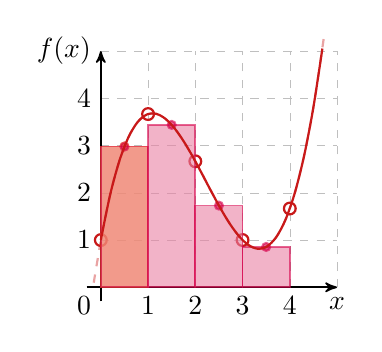
\begin{tikzpicture}[scale=0.6]
        \draw[gridline,step=1] (0,0) grid (5,5);
  \coordinate (O) at (0,0);
  % Axes
  \draw[line,->] (-0.3,0) -- (5,0) coordinate[label = {below:$x$}] (xmax);
  \draw[line,->] (0,-0.3) -- (0,5) coordinate[label = {left:$f(x)$}] (ymax);
  
  % Labels
  \draw (0,0) node[below left]{$0$};
  \foreach \s in {1,...,4}
  {
    \draw (\s,0) node[below]{$\s$};
    \draw (0,\s) node[left]{$\s$};
    }
    
    % Title
    %       \draw (2.5,5) node[above]{$f(x)=\frac{x^3}{2}-\frac{10x^2}{3}+\frac{11x}{2}+1$};
    
    % Plots
    \node[interp] (x0) at (0,1) {};
    \node[interp] (x1) at (1,3.667) {};
    \node[interp] (x2) at (2,2.667) {};
    \node[interp] (x3) at (3,1) {};
    \node[interp] (x4) at (4,1.667) {};
    \node (bb) at (5,5.3) {};
%       \draw [graph,domain=0:4.69] plot (\x, {0.5*\x*\x*\x-(10/3)*\x*\x+5.5*\x+1});
%       \draw [graph,opacity=0.4,dashed,domain=-0.15:4.73] plot (\x, {0.5*\x*\x*\x-(10/3)*\x*\x+5.5*\x+1});

      
      \draw<2> [intblock,draw=tueorange,fill=tueorange] (0,0) rectangle (1,2.9792);
      \node<2> [intdot,draw=tueorange,fill=tueorange] at (0.5, 2.9792) {};
      \draw<1> [intblock] (0,0) rectangle (1,2.9792);
      \node<1> [intdot] at (0.5, 2.9792) {};
      \draw<1> [intblock] (1,0) rectangle (2,3.4375);
      \node<1> [intdot] at (1.5, 3.4375) {};
      \draw<1> [intblock] (2,0) rectangle (3,1.7292);
      \node<1> [intdot] at (2.5, 1.7292) {};
%       \draw<1> [intblock] (3,0) rectangle (4,0.8542);
%       \node<1> [intdot] at (3.5, 0.8542) {};
      \draw [intblock] (3,0) rectangle (4,0.8542);
      \node [intdot] at (3.5, 0.8542) {};
      
      \draw [interp,smooth,domain=0:4.69] plot (\x, {0.5*\x*\x*\x-(10/3)*\x*\x+5.5*\x+1});
      \draw [interp,smooth,opacity=0.4,dashed,domain=-0.15:4.73] plot (\x, {0.5*\x*\x*\x-(10/3)*\x*\x+5.5*\x+1});
    \end{tikzpicture}
  \column{0.5\textwidth}
  \centering Trapezoid rule
    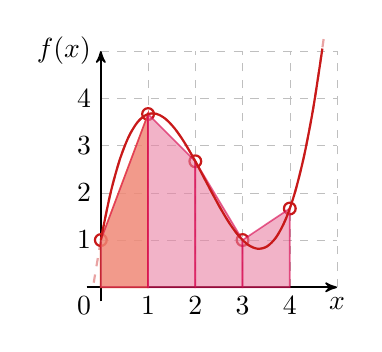
\begin{tikzpicture}[scale=0.6]
        \draw[gridline,step=1] (0,0) grid (5,5);
  \coordinate (O) at (0,0);
  % Axes
  \draw[line,->] (-0.3,0) -- (5,0) coordinate[label = {below:$x$}] (xmax);
  \draw[line,->] (0,-0.3) -- (0,5) coordinate[label = {left:$f(x)$}] (ymax);
  
  % Labels
  \draw (0,0) node[below left]{$0$};
  \foreach \s in {1,...,4}
  {
    \draw (\s,0) node[below]{$\s$};
    \draw (0,\s) node[left]{$\s$};
    }
    
    % Title
    %       \draw (2.5,5) node[above]{$f(x)=\frac{x^3}{2}-\frac{10x^2}{3}+\frac{11x}{2}+1$};
    
    % Plots
    \node[interp] (x0) at (0,1) {};
    \node[interp] (x1) at (1,3.667) {};
    \node[interp] (x2) at (2,2.667) {};
    \node[interp] (x3) at (3,1) {};
    \node[interp] (x4) at (4,1.667) {};
    \node (bb) at (5,5.3) {};
%       \draw [graph,domain=0:4.69] plot (\x, {0.5*\x*\x*\x-(10/3)*\x*\x+5.5*\x+1});
%       \draw [graph,opacity=0.4,dashed,domain=-0.15:4.73] plot (\x, {0.5*\x*\x*\x-(10/3)*\x*\x+5.5*\x+1});

      \draw<2> [intblock,draw=tueorange,fill=tueorange] (0,0) -- (1,0) -- (x1.center) -- (x0.center) -- cycle;
      \draw<1> [intblock] (0,0) -- (1,0) -- (x1.center) -- (x0.center) -- cycle;
      \draw<1> [intblock] (1,0) -- (2,0) -- (x2.center) -- (x1.center) -- cycle;
      \draw<1> [intblock] (2,0) -- (3,0) -- (x3.center) -- (x2.center) -- cycle;
%       \draw<1> [intblock] (3,0) -- (4,0) -- (x4.center) -- (x3.center) -- cycle;
      \draw [intblock] (3,0) -- (4,0) -- (x4.center) -- (x3.center) -- cycle;
      
      \draw [interp,smooth,domain=0:4.69] plot (\x, {0.5*\x*\x*\x-(10/3)*\x*\x+5.5*\x+1});
      \draw [interp,smooth,opacity=0.4,dashed,domain=-0.15:4.73] plot (\x, {0.5*\x*\x*\x-(10/3)*\x*\x+5.5*\x+1});
  \end{tikzpicture}
  \end{columns}
  \pause
  \tikz{\node[emphblock,text width=\textwidth]{\color{tueorange}In convex parts (bending down), the midpoint rule tends to overestimate the integral (trapezoid underestimates). \color{tuefuchsia}In concave parts (bending up), the midpoint rule tends to underestimate the integral (trapezoid overestimates).};}
\end{frame}

\begin{frame}
  \frametitle{Towards higher-order integration}
  The errors of the midpoint rule and trapezoid rule behave in a similar way, but have opposite signs.
  \begin{itemize}
    \item Midpoint: $\displaystyle \abs{I - M_n} \leq \frac{f^{(2)}_\text{max}(b - a)^3}{24n^2}$
    \item Trapezoid: $\displaystyle \abs{I - T_n} \leq \frac{f^{(2)}_\text{max} (b-a)^3}{12n^2}$
  \end{itemize}
  \pause
  For a quadratic function, the errors relate as:
  \[
    \abs{I-M_n} = \frac{1}{2}\abs{I-T_n} 
  \]
  \pause
  Taking the weighted average of these two yields the Simpson's rule:
  \[
    S_{2n} = \frac{2}{3}M_n + \frac{1}{3}T_n
  \]
  The $2n$ means we have $2n$ subintervals: the $n$ trapezoid intervals are subdivided by the midpoint rule.
\end{frame}

\begin{frame}
  \frametitle{Simpson's rule}
  Consider the interval $i\in[x_0,x_2]$, subdivided in three equidistant interpolation points: $x_0,x_1,x_2$. \vskip1ex
  \begin{itemize}
    \item Midpoint: $\displaystyle M_i = f(\frac{x_0+x_2}{2})2\Delta x = f(x_1)2\Delta x$
    \item Trapezoid: $\displaystyle T_i = \frac{f(x_0)+f(x_2)}{2}2\Delta x$
    \item Simpson:  $\displaystyle S_i = \frac{2}{3}M_i + \frac{1}{3}T_i$
  \end{itemize}
  Note that $M_i$ and $T_i$ were computed on interval $x_2-x_0=2\Delta x$. 
  \vskip1ex \pause
  Now we have:
  \begin{align*}
    S_i &= \frac{2}{3}\left[f(x_1)2\Delta x\right] + \frac{1}{3}\left[\frac{f(x_0)+f(x_2)}{2}2\Delta x\right] \\
    &= \frac{4\Delta x}{3}f(x_1) + \frac{\Delta x}{3}f(x_0)+f(x_2)
    \onslide<3>{=\color{tuered} \frac{\Delta x}{3}\left( f(x_0) + 4f(x_1) + f(x_2)\right)}
  \end{align*}
\end{frame}

\begin{frame}
  \frametitle{Simpson's rule}
  We write $f(x_k) = f_k$. The integral of an interval $i\in[x_0,x_2]$ is approximated as:
  \[
    S_i = \frac{\Delta x}{3}\left( f_0 + 4f_1 + f_2\right)
  \]
  \pause
  The next interval, $S_{j}$ with $j\in[x_2,x_4]$ with midpoint $x_3=\frac{x_2+x_4}{2}$ is approximated as:
  \[
    S_j = \frac{\Delta x}{3}\left( f_2 + 4f_3 + f_4\right)
  \]
  \pause
  If we sum these two intervals we obtain:
  \begin{align*}
    I \approx S_i + S_j &= \left[\frac{\Delta x}{3}\left( f_0 + 4f_1 + f_2\right)\right] +  \left[\frac{\Delta x}{3}\left( f_2 + 4f_3 + f_4\right)\right] \\
    &= \frac{\Delta x}{3}\left(f_0 + 4f_1+2f_2 +4f_3 + f4 \right)
  \end{align*}
\end{frame}
\begin{frame}
  \frametitle{Simpson's rule}
  \rowcolors[]{50}{white}{white}
  In general, Simpson's rule can be written as:
%   \hspace*{-2em}
  \begin{flalign*}
    \int_a^b f(x)dx &\approx \sum^n_{\begin{matrix}
                             k=2 & \\
                             k\, \text{even}
                           \end{matrix}} \frac{\Delta x}{3}\left( f_{k-2} + 4f_{k-1} + f_k\right) &\\
                           &= \frac{\Delta x}{3}\left(f_0 + 4f_1 +2f_2+4f_3+2f_4+\ldots+2f_{n-2}+4f_{n-1}+f_n \right) &
  \end{flalign*}
  \pause
  The error is given by:
  \[
    \abs{I-S_n} \leq \frac{f^{(4)}_\text{max}(b-a)^5}{180n^4}
  \]
  if integrand $f$ is differentiable on $[a,b]$.
\end{frame}

\begin{frame}
  \frametitle{Simpson's rule: example}
  \footnotesize\selectfont
  Recall our example data, described by $f(x)=\frac{x^3}{2}-\frac{10x^2}{3}+\frac{11x}{2}+1$ \\
  $ I = \int_0^4 \frac{x^3}{2}-\frac{10x^2}{3}+\frac{11x}{2}+1 = \frac{80}{9} \approx 8.888\ldots$
  \begin{columns}
    \column{0.5\textwidth}
    \begin{itemize}
      \item<2-> \color{tuered}Interpolating $x_0$, $x_1$ and $x_2$:  $ p_{2a}(x) = -\frac{11}{6}x^2+4\frac{1}{2}x+1 $ \\
      $\int_0^2 p_{2a} = \frac{55}{9} \approx 6.1111$
      \item<3-> \color{tuelblue} Interpolating $x_2$, $x_3$ and $x_4$: $ p_{2b}(x) = \frac{7x^2}{6}-7\frac{1}{2}x+13 $ \\
      $\int_2^4 p_{2b} = \frac{25}{9} \approx 2.777\ldots$
      \item<4-> Adding the separate integrals: \\
      $\int_0^2 p_{2a} + \int_2^4 p_{2b} = \frac{80}{9}$
    \end{itemize}
    \column{0.50\textwidth}
    \centering
    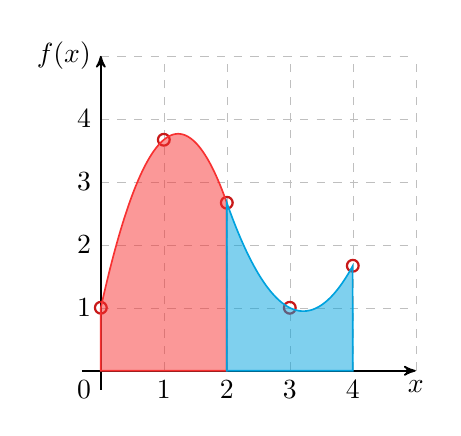
\begin{tikzpicture}[domain=-1:6,scale=0.8]
        \draw[gridline,step=1] (0,0) grid (5,5);
  \coordinate (O) at (0,0);
  % Axes
  \draw[line,->] (-0.3,0) -- (5,0) coordinate[label = {below:$x$}] (xmax);
  \draw[line,->] (0,-0.3) -- (0,5) coordinate[label = {left:$f(x)$}] (ymax);
  
  % Labels
  \draw (0,0) node[below left]{$0$};
  \foreach \s in {1,...,4}
  {
    \draw (\s,0) node[below]{$\s$};
    \draw (0,\s) node[left]{$\s$};
    }
    
    % Title
    %       \draw (2.5,5) node[above]{$f(x)=\frac{x^3}{2}-\frac{10x^2}{3}+\frac{11x}{2}+1$};
    
    % Plots
    \node[interp] (x0) at (0,1) {};
    \node[interp] (x1) at (1,3.667) {};
    \node[interp] (x2) at (2,2.667) {};
    \node[interp] (x3) at (3,1) {};
    \node[interp] (x4) at (4,1.667) {};
    \node (bb) at (5,5.3) {};
%       \draw [graph,domain=0:4.69] plot (\x, {0.5*\x*\x*\x-(10/3)*\x*\x+5.5*\x+1});
%       \draw [graph,opacity=0.4,dashed,domain=-0.15:4.73] plot (\x, {0.5*\x*\x*\x-(10/3)*\x*\x+5.5*\x+1});

      % Polynomial interpolant
      \draw<2->[graph,domain=0:2,draw=tuered,fill=tuered,fill opacity=0.5] (0,0) -- plot (\x, {-(11/6)*\x*\x+(4.5)*\x+1}) -- (2,0) -- cycle;
      \draw<3->[graph,domain=2:4,draw=tuelblue,fill=tuelblue,fill opacity=0.5] (2,0) -- plot (\x, {(7/6)*\x*\x-7.5*\x + 13}) -- (4,0) -- cycle;
    \end{tikzpicture}
  \end{columns}
  \onslide<5->{
  Using Simpson's rule:
  $ I \approx \frac{\Delta x}{3}\left(f_0 + 4f_1 +2f_2+4f_3+f_4 \right) = \frac{1}{3}\left(1+4\cdot3.6667+2\cdot2.6667+4\cdot1.0000+1.6667\right) = 8.88888 = \frac{80}{9}$
  }
  \onslide<6>{\tikz{\node[emphblock,text width=\textwidth]{Simpson's method is of fourth order, and it gives exact approximations of third order polynomials!};}}
\end{frame}

\begin{frame}[fragile]
  \frametitle{Integration in Matlab}
  Integration can be done numerically in Matlab.
  \begin{itemize}
    \item \lstinline$trapz(x,y)$ uses the trapezoid rule to integrate the data. Make sure you use the \lstinline$x$ variable if your data is not spaced with $\Delta x=1$. Can handle non-equidistant data.
    \item Integration of functions can be done using the \lstinline$integral(fun,xmin,xmax)$ function:
    \begin{lstlisting}
fun = @(x) exp(-x.^2);
I = integral(fun,0,10)
I =
   0.886226925452758
    \end{lstlisting}
  \end{itemize}
\end{frame}

\section{Conclusion}
\againframe<2>{contents_integration}
\begin{frame}
  \frametitle{What hasn't been discussed?}
  This course is by no means complete, and further reading is possible.
   \begin{itemize}
      \item Legendre polynomials: Another way of performing the polynomial interpolation
      \item Gaussian quadrature: A third-order integration method that requires only two base points (in contrast to the third order Simpson's method, which requires three points)
      \item Adaptive techniques: Parts of a function that are relatively steady (no wild oscillations) and differentiable can be integrated with much larger step sizes than other parts of the function.
      \item Simpson's 3/8-rule: Yet another integration technique, requiring an additional data point
   \end{itemize}
\end{frame}

\begin{frame}
  \frametitle{Summary}
  \begin{itemize}
    \item Interpolation is used to obtain data between existing data points
    \begin{itemize}
      \item (Bi-)Linear, polynomial and spline interpolation methods
      \item Construction of Newton polynomials
      \item Oscillations of high-order polynomials
    \end{itemize}
    \item Several techniques for numerical integration were discussed:
    \begin{itemize}
      \item Riemann sums, trapezoid rule, Simpson's rule
      \item Upper-bound errors were given for each technique
    \end{itemize}
  \end{itemize}
\end{frame}

\title{Ordinary differential equations 1}
\subtitle{Explicit techniques for ODEs}
\lecture{ODE 1}{ode1}
\part{Ordinary differential equations I - Explicit methods}
\section{Introduction}
\subsection*{General}
\begin{frame}[label=contents_ode1]
  \frametitle{Today's outline}
  \mode<beamer>{
    \only<1>{\tableofcontents}
  }
  \only<2>{\tableofcontents[currentsection]}
\end{frame}
 
\begin{frame}
  \frametitle{Overview}
    \begin{block}{Ordinary differential equations}
      An equation containing a function of one independent variable and its derivatives, in contrast to a \emph{partial differential equation}, which contains derivatives with respect to more independent variables.
    \end{block}
    \pause
  \begin{block}{Main question}
  How to solve 
  \[
    \frac{d\vec{y}}{dx} = f(\vec{y}(x),x) \quad \text{with} \quad \vec{y}(x=0) = \vec{y}_0
  \]
  accurately and efficiently?
  \end{block}
\end{frame}

\begin{frame}
  \frametitle{What is an ODE?}
  \begin{itemize}
    \item Algebraic equation:
    \[
      f(y(x),x) = 0 \qquad \text{e.g.} \, -\ln(K_{eq})=(1-\zeta)
    \]
    \item First order ODE:
    \[
      f\left(\frac{dy}{dx}(x),y(x),x\right) = 0 \quad \text{e.g.} \, \frac{dc}{dt} = -kc^n
    \]
    \item Second order ODE:
    \[
      f\left(\frac{d^2y}{dx^2}(x),\frac{dy}{dx}(x),y(x),x \right) = 0 \quad \text{e.g.} \quad \mathcal{D}\frac{d^2c}{dx^2}= - \frac{kc}{1+Kc}
    \]
  \end{itemize}
\end{frame}

\begin{frame}
  \frametitle{About second order ODEs}
  Very often a second order ODE can be rewritten into a system of first order ODEs (whether it is handy depends on the boundary conditions!)
  \vskip1em
  \pause
  \mode<beamer>{
  \only<1-2>{
  \begin{block}{Example}
  Recall:
  \[
    \mathcal{D}\frac{d^2c}{dx^2}= - \frac{kc}{1+Kc}
  \]
  Define $y = -\mathcal{D} \frac{dc}{dx}$, then $\frac{dy}{dx}=\frac{kc}{1+Kc}$, thus solve system:
  \begin{align*}
    \frac{dc}{dx} &= -\frac{1}{\mathcal{D}}y \\
    \frac{dy}{dx} &= \frac{kc}{1+Kc}
  \end{align*}
  \end{block}}}
  \only<3>{
  \begin{block}{More general}
  Consider the second order ODE:
  \[
    \frac{d^2y}{dx^2} + q(x)\frac{dy}{dx} = r(x)
  \]
  Now define and solve using $z$ as a new variable:
  \begin{align*}
    \frac{dy}{dx} &= z(x) \\
    \frac{dz}{dx} &= r(x) - q(x)z(x)
  \end{align*}
  \end{block}}
  \vskip1em
  \pause
\end{frame}

\begin{frame}[label=ivpbvp]
  \frametitle{Importance of boundary conditions}
  \footnotesize\selectfont
  The nature of boundary conditions determines the appropriate numerical method. Classification into 2 main categories:
  \begin{itemize}
    \item \emph{Initial value problems (IVP)} \\
    We know the values of all $y_i$ at some starting position $x_s$, and it is desired to find the values of $y_i$ at some final point $x_f$. \vskip1em
    \begin{center}
      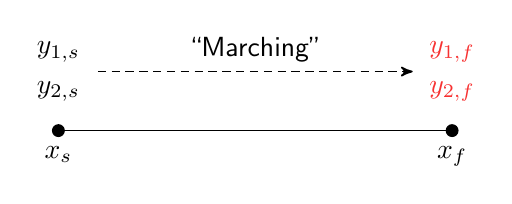
\begin{tikzpicture}[scale=5]
        \node[] (y1s) at (0,0.1) {$y_{1,s}$};
        \node[] (y1f) at (1,0.1) {\color{tuered}$y_{1,f}$};
        \node[] (y2s) at (0,0) {$y_{2,s}$};
        \node[] (y2f) at (1,0) {\color{tuered}$y_{2,f}$};
        \node[fdot] (xs) at (0,-0.1) {};
        \node[fdot] (xf) at (1,-0.1) {};
        \node[anchor=north] at (xs.south) {$x_s$};
        \node[anchor=north] at (xf.south) {$x_f$};
        \draw[line] (xs) -- (xf);
        \draw[line,->,densely dashed] (0.1,0.05) -- node[midway,above] {``Marching''} (0.9,0.05);
      \end{tikzpicture}
    \end{center}
    \item \emph{Boundary value problems (BVP)} \\
    Boundary conditions are specified at more than one $x$. Typically, some of the BC are specified at $x_s$ and the remainder at $x_f$. \vskip1em
    \centering
    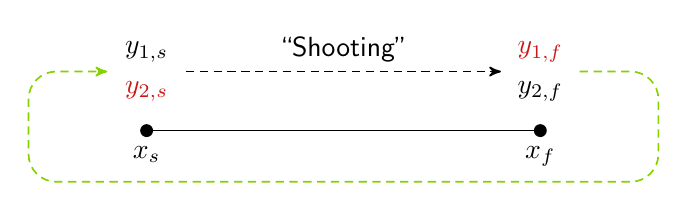
\begin{tikzpicture}[scale=5]
      \node[] (y1s) at (0,0.1) {$y_{1,s}$};
\node[] (y1f) at (1,0.1) {\color{scharlaken}$y_{1,f}$};
\node[] (y2s) at (0,0) {\color{scharlaken}$y_{2,s}$};
\node[] (y2f) at (1,0) {$y_{2,f}$};
\node[fdot] (xs) at (0,-0.1) {};
\node[fdot] (xf) at (1,-0.1) {};
\node[anchor=north] at (xs.south) {$x_s$};
\node[anchor=north] at (xf.south) {$x_f$};
\draw[line] (xs) -- (xf);
\draw[line,->,densely dashed] (0.1,0.05) -- node[midway,above] {``Shooting''} (0.9,0.05);

\coordinate[] (b) at ($(y1f)!0.5!(y2f) + (0.1,0) $) {};
\coordinate[right of=b] (c1) {};
\coordinate[below=1.4cm] (c2) at (c1)  {};
%       \coordinate[below of=1cm] at (c2) (c5) {};

\coordinate[] (s) at ($(y1s)!0.5!(y2s) - (0.1,0) $) {};
\coordinate[left of=s] (c3) {};
\coordinate[below=1.4cm] (c4) at (c3)  {};
%       \coordinate[below of=c4] (c6) {};

%       \node[] (b) at ($(y1f)!0.5!(y2f)$) {};
\draw[line,->,densely dashed,draw=tuegreen,rounded corners=10pt] (b) -- (c1) -- (c2) -- (c4) -- (c3) -- (s);
%       \draw[line,densely dashed,draw=tuegreen] (y2f) to [controls=(1,-0.2) and +(-0.1,-0.2)] (y2s);
    \end{tikzpicture}
  \end{itemize}
\end{frame}

\begin{frame}
  \frametitle{Overview}
  Initial value problems:
  \begin{itemize}
    \colorize<2> \item Explicit methods
    \begin{itemize}
      \colorize<2> \item First order: forward Euler
      \colorize<2> \item Second order: improved Euler (RK2)
      \colorize<2> \item Fourth order: Runge-Kutta 4 (RK4)
      \colorize<2> \item Step size control
    \end{itemize}
    \colorize<3> \item Implicit methods
    \begin{itemize}
      \colorize<3> \item First order: backward Euler
      \colorize<3> \item Second order: midpoint rule
    \end{itemize}
  \end{itemize}
  \onslide<4>{
  Boundary value problems
  \begin{itemize}
    \colorize<4> \item Shooting method
  \end{itemize}
  }
\end{frame}

\section{Euler's method}
\againframe<2>{contents_ode1}
\subsection{Forward Euler}
\begin{frame}
  \frametitle{Euler's method}
  Consider the following single initial value problem:
  \[
    \frac{dc}{dt} = f(c(t),t) \quad \text{with} \quad c(t=0)=c_0 \quad \text{(initial value problem)}
  \]
  \pause
  Easiest solution algorithm: Euler's method, derived here via Taylor series expansion:
  \[
    c(t_0 + \Delta t) \approx c(t_0) + \left.\frac{dc}{dt}\right|_{t_0}\Delta t + \frac{1}{2} \left.\frac{d^2c}{dt^2}\right|_{t_0} \left(\Delta t\right) ^2 + \mathcal{O}{(\Delta t^3)}
  \]
  \pause
  Neglect terms with higher order than two: $\left. \frac{dc}{dt}\right|_{t_0} = \frac{c(t_0 + \Delta t) - c(t_0)}{\Delta t}$
  Substitution: 
  \[
    \frac{c(t_0 + \Delta t) - c(t_0)}{\Delta t} = f(c_0,t_0)\Rightarrow c(t_0+\Delta t) = c(t_0) + \Delta t f(c_0,t_0) 
  \]
\end{frame}

\begin{frame}[t,fragile]
  \frametitle{Euler's method: graphical example}
  \[
    \frac{c(t_0 + \Delta t) - c(t_0)}{\Delta t} = f(c_0,t_0)\Rightarrow c(t_0+\Delta t) = c(t_0) + \Delta t f(c_0,t_0) 
  \]
  \vskip1em
   \begin{tikzpicture}
      \begin{axis}[every axis/.append style={font=\footnotesize},
      width=\columnwidth, height=5.5cm,
      xmin=0,xmax=4,ymin=0,ymax=4,
      xtick={1,2,3},ytick={1,2,2.5},
      axis x line=middle,axis y line=middle,
      xlabel=$t$,xticklabels={$t_0$,$\Delta t$,$2\Delta t$},
      ylabel=$c(t)$,yticklabels={$c_0$,$c_1$,$c_2$},tick align=outside,ymajorgrids=true,major grid style={dashed}]
 
    \addplot[graph,quiver={u=\thisrow{u},v=\thisrow{v},scale arrows=0.4},-stealth']
      table {
      x y u v
      1 1 1 1
      2 2 1 0.5
      };
      \addplot[graph,sharp plot,densely dashed,mark=*,mark options={solid,fill=tuered},mark size=1.7pt,nodes near coords={\coordindex}]
      table {
      x y
      1 1
      2 2
      3 2.5
      };
      \node[black] at (axis cs:1.4,0.9) {$\left.\frac{dc}{dt}\right|_{t_0}$};
      \node[black] at (axis cs:2.4,1.8) {$\left.\frac{dc}{dt}\right|_{\Delta t}$};
%       \node[black] at (axis cs:2.1,0.5) {$k_1$};
    \end{axis}
  \end{tikzpicture}
\end{frame}

\begin{frame}
  \frametitle{Euler's method - solution method}
    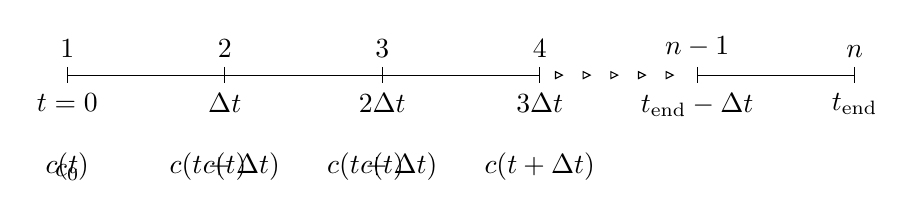
\begin{tikzpicture}[]
    %draw horizontal line   
    \draw (0,0) -- (6,0);
    \draw[decorate,decoration=triangles] (6.2,0) -- (8.0,0);
    \draw (8,0) -- (10,0);

    %draw vertical lines
    \foreach \x in {0,2,4,6,8,10}
      \draw (\x cm,3pt) -- (\x cm,-3pt);

    %draw nodes
    \draw (0,0) node[below=3pt] {$ t=0 $} node[above=3pt] {$ 1 $};
    \draw (2,0) node[below=3pt] {$ \Delta t $} node[above=3pt] {$ 2 $};
    \draw (4,0) node[below=3pt] {$ 2\Delta t $} node[above=3pt] {$ 3 $};
    \draw (6,0) node[below=3pt] {$ 3\Delta t $} node[above=3pt] {$ 4 $};
    \draw (8,0) node[below=3pt] {$ t_\mathrm{end}-\Delta t $} node[above=3pt] {$ n-1 $};
    \draw (10,0) node[below=3pt] {$ t_\mathrm{end} $} node[above=3pt] {$ n $};
    
    \onslide<1>{
      \draw (0,-1.5) node[above=1pt] {$c_0$};
    }
    \onslide<2>{
      \draw (0,-1.5) node[above=1pt] {$c(t)$};
      \draw (2,-1.5) node[above=1pt] {$c(t+\Delta t)$};
    }
    \onslide<3>{
      \draw (2,-1.5) node[above=1pt] {$c(t)$};
      \draw (4,-1.5) node[above=1pt] {$c(t+\Delta t)$};
    }
    \onslide<4>{
      \draw (4,-1.5) node[above=1pt] {$c(t)$};
      \draw (6,-1.5) node[above=1pt] {$c(t+\Delta t)$};
    }
   \end{tikzpicture}
   \vskip1em
  Start with $t = t_0$, $c=c_0$, then calculate at discrete points in time: $c(t_1 = t_0 + \Delta t) = c(t_0) + \Delta t f(c_0,t_0)$. 
  \onslide<5>{
  \vskip1em
  \tikz{\node[emphblock,text width=\textwidth] {
  Pseudo-code Euler's method: $ \frac{dy}{dx} = f(x,y) \quad \text{and} \quad y(x_0) = y_0$.
  \begin{enumerate}
    \item Initialize variables, functions; set $h = \frac{x_1 - x_0}{N}$
    \item Set $x = x_0$, $y = y_0$
    \item While $x<x_\text{end}$ do\\
    $ \displaystyle x_{i+1} = x_i + h; \quad y_{i+1} = y_i + h f(x_i,y_i)$
  \end{enumerate}
  };}
  }
\end{frame}

\begin{frame}
  \frametitle{Euler's method - example}
  First order reaction in a batch reactor:
  \[
    \frac{dc}{dt} = -kc \quad \text{with} \quad c(t=0) = 1\, \si{\mole\per\cubic\meter}, \quad k = 1\, \si{s^{-1}}, \quad t_\text{end} = 2\, \si{\second}
  \]
  \pause
  \footnotesize\selectfont
  \begin{longtable}{p{0.3\textwidth}p{0.5\textwidth}}
  \hline
    Time [\si{\second}] & Concentration [\si{\mole\per\cubic\meter}] \\ \hline
    $t_0 = 0$                                 & $c_0 = 1.00$ \\
    $\begin{aligned}t_1 &= t_0 + \Delta t\\ &= 0 + 0.1 = 0.1\end{aligned}$    & $\begin{aligned}c_1 &= c_0 + \Delta t \cdot (-kc_0) \\ &= 1 + 0.1 \cdot (-1 \cdot 1) = 0.9\end{aligned}$ \\
    $\begin{aligned}t_2 &= t_1 + \Delta t\\ &= 0.1 + 0.1 = 0.2\end{aligned}$  & $\begin{aligned}c_2 &= c_1 + \Delta t \cdot (-kc_1)\\ &= 0.9 + 0.1 \cdot (-1 \cdot 0.9) = 0.81\end{aligned}$ \\ 
    $\begin{aligned} t_3 &= t_2 + \Delta t \\ &= 0.2 + 0.1 = 0.3\end{aligned}$  & $\begin{aligned}c_3 &= c_2 + \Delta t \cdot (-kc_2)\\ &= 0.81 + 0.1 \cdot (-1 \cdot 0.81) = 0.729 \end{aligned}$ \\ 
    \centering$\ldots$                                  & $\quad \quad \quad \quad \ldots$ \\
    $t_{i+1} = t_i + \Delta t$                & $c_{i+1} = c_i + \Delta t \cdot (-k c_i) $ \\
    \centering$\ldots$ & $\quad \quad \quad \quad \ldots$ \\
    $t_{20} = 2.0 $ & $c_{20} = c_{19} + \Delta t \cdot (-k c_{19}) = 0.121577$ \\
    \hline
  \end{longtable}
\end{frame}

\begin{frame}
  \frametitle{Euler's method - example}
%   Accuracy: Results are shown for $N=20,4-,80,\ldots,320$ using $k = 1 \si{s^{-1}$
  \begin{center}
    \begin{tikzpicture}
      \begin{axis}[every axis/.append style={font=\footnotesize},
    width=\textwidth, height=7cm,     % size of the image
    grid = major,
    grid style={dashed, gray!30},
    xmin=0,     % start the diagram at this x-coordinate
    xmax=2,    % end   the diagram at this x-coordinate
    ymin=0,     % start the diagram at this y-coordinate
    ymax=1,   % end   the diagram at this y-coordinate
    xtick={0,0.2,...,2},
    ytick={0,0.2,...,1},
    axis background/.style={fill=white},
    axis x line=middle,
    axis y line=middle,
    ylabel style={at={(ticklabel* cs:1.05)},anchor=south west},
    ylabel=$c$ (\si{\mole\per\cubic\meter}),
    xlabel=$t$ (\si{\second}),
    tick align=outside,
    legend style={draw=none,fill=none,font=\tiny,at={(0.5,1.0)},anchor=south},
    legend columns=5
    ]

      \addplot[graph,mark=x] table [id=EE_20]{data/ODE_EulerExpl_20.dat};  \addlegendentry{20 points}
      \only<2->{\addplot[graph,draw=tueyellow] table [id=EE_20]{data/ODE_EulerExpl_40.dat}; } \addlegendentry{40 points}
      \only<3->{\addplot[graph,draw=tuelblue] table [id=EE_20]{data/ODE_EulerExpl_80.dat}; } \addlegendentry{80 points}
      \only<4->{\addplot[graph,draw=tuegreen] table [id=EE_20]{data/ODE_EulerExpl_160.dat};} \addlegendentry{160 points}
      \only<5->{\addplot[graph,draw=tuelila] table [id=EE_20]{data/ODE_EulerExpl_320.dat};} \addlegendentry{320 points}
    \end{axis}
    \end{tikzpicture}
  \end{center}
\end{frame}

{\nologo
\begin{frame}
  \frametitle{Problems with Euler's method}
  The question is: What step size, or how many steps to use?
  \begin{enumerate}
    \item \emph{Accuracy}  $\Rightarrow$ need information on numerical error!
    \item \emph{Stability} $\Rightarrow$ need information on stability limits!
  \end{enumerate}
  \vskip1em

  \begin{columns}
    \column{0.5\textwidth}
    \begin{tikzpicture}
      \begin{axis}[every axis/.append style={font=\tiny},
      width=\columnwidth, height=5.5cm,     % size of the image
      grid = major,
      grid style={dashed, gray!30},
      xmin=0,     % start the diagram at this x-coordinate
      xmax=2,    % end   the diagram at this x-coordinate
      ymin=0,     % start the diagram at this y-coordinate
      ymax=1,   % end   the diagram at this y-coordinate
      xtick={0,0.5,...,2},
      ytick={0,0.25,...,1},
%       axis background/.style={fill=white},
%       axis x line=middle,
%       axis y line=middle,
      xlabel style={at={(ticklabel* cs:1.1)},anchor=south},
      xlabel=$t$ (\si{\second}),
      ylabel style={at={(yticklabel* cs:0.7)},anchor=north,left=7mm},
      ylabel=$c$ (\si{\mole\per\cubic\meter}),
      tick align=outside,
      legend style={draw=none,fill=none,font=\tiny,at={(0.5,-0.1)},anchor=north},
      legend columns=3
      ]

	\addplot[graph] table [id=EE_20]{data/ODE_EulerExpl_20.dat}; \addlegendentry{$N=20$}
	\addplot[graph,draw=tueyellow] table [id=EE_20]{data/ODE_EulerExpl_40.dat}; \addlegendentry{$N=40$}
	\addplot[graph,draw=tuelblue] table [id=EE_20]{data/ODE_EulerExpl_80.dat};  \addlegendentry{$N=80$}
	\addplot[graph,draw=tuegreen] table [id=EE_20]{data/ODE_EulerExpl_160.dat}; \addlegendentry{$N=160$}
	\addplot[graph,draw=tuelila] table [id=EE_20]{data/ODE_EulerExpl_320.dat}; \addlegendentry{$N=320$}
      \end{axis}
    \end{tikzpicture}
     \centering Reaction rate: $k = 1$ \si{s^{-1}}
    \column{0.5\textwidth}
    \begin{tikzpicture}
      \begin{axis}[every axis/.append style={font=\tiny},
      width=\columnwidth, height=5.5cm,     % size of the image
      grid = major,
      grid style={dashed, gray!30},
      xmin=0,     % start the diagram at this x-coordinate
      xmax=0.25,    % end   the diagram at this x-coordinate
      ymin=-5,     % start the diagram at this y-coordinate
      ymax=5,   % end   the diagram at this y-coordinate
      restrict y to domain*=-300:300,
      xtick={0,0.05,...,0.25},
      ytick={-5,-2.5,...,5},
%       axis background/.style={fill=white},
% %       axis x line=middle,
%       axis y line=middle,
      xlabel style={at={(ticklabel* cs:1.1)},anchor=south},
      xlabel=$t$ (\si{\second}),
      ylabel style={at={(yticklabel* cs:0.7)},anchor=north,left=7mm},
      ylabel=$c$ (\si{\mole\per\cubic\meter}),
      tick align=outside,
      legend style={draw=none,fill=none,font=\tiny,at={(0.5,-0.1)},anchor=north},
      legend columns=3
      ]

	\addplot[graph,sharp plot,mark=+,mark size=1.3pt] table [id=EE_20]{data/ODE_Euler2Expl_20.dat}; \addlegendentry{$N=20$}
	\addplot[graph,sharp plot,draw=tueyellow,mark=x,mark size=1.3pt] table [id=EE_20]{data/ODE_Euler2Expl_40.dat}; \addlegendentry{$N=40$}
	\addplot[graph,sharp plot,draw=tuelblue,mark=o,mark size=1.3pt] table [id=EE_20]{data/ODE_Euler2Expl_80.dat};  \addlegendentry{$N=80$}
	\addplot[graph,sharp plot,draw=tuegreen] table [id=EE_20]{data/ODE_Euler2Expl_160.dat}; \addlegendentry{$N=160$}
	\addplot[graph,sharp plot,draw=tuelila] table [id=EE_20]{data/ODE_Euler2Expl_320.dat}; \addlegendentry{$N=320$}
      \end{axis}
    \end{tikzpicture}
     \centering Reaction rate: $k = 50$ \si{s^{-1}}
  \end{columns}
\end{frame}
}

\begin{frame}
  \frametitle{Accuracy}
  Comparison with analytical solution for $k=1$ \si{s^{-1}}:
  \[
    c(t) = c_0 \exp \left(-kt\right) \Rightarrow \zeta = 1-\exp\left(-kt\right) \Rightarrow \zeta_\text{analytical} = 0.864665
  \]
  \begin{columns}[T]
    \column{0.5\textwidth}
      \begin{longtable}{ccc}
      \hline
      $N$ & $\zeta$ & $\frac{\zeta^{}_\text{numerical}-\zeta_\text{analytical}}{\zeta_\text{analytical}}$ \\ \hline
      20  & 0.878423 & 0.015912 \\
      40  & 0.871488 & 0.007891 \\
      80  & 0.868062 & 0.003929 \\
      160 & 0.866360 & 0.001961 \\
      320 & 0.865511 & 0.000979\\
      \hline
    \end{longtable}
  \column{0.5\textwidth}
    \begin{tikzpicture}
      \begin{loglogaxis}[
      width=\columnwidth,height=5cm,
      ylabel style={at={(yticklabel* cs:0.83)},anchor=south,left=13mm},
      xlabel=N,
      ylabel=Relative error,
      log ticks with fixed point,
      xtick={20,40,80,160,320},
      ytick={0.02,0.01,0.005,0.002,0.001}]
      \addplot[graph,draw=tuelblue,mark=o] table {data/ODE_euler_err.dat};
      \end{loglogaxis}
    \end{tikzpicture}
  \end{columns}
\end{frame}

\begin{frame}
  \frametitle{Accuracy}
  \tikz{\node[emphblock,text width=\textwidth] {For Euler's method: Error halves when the number of grid points is doubled, i.e. error is proportional to $\Delta t$: first order method.};}
  \vskip1em
  Error estimate:
  \[
    \left. \frac{dx}{dt}\right|_{t_0} = \frac{x(t_0+\Delta t)-x(t_0)}{\Delta t} + \frac{1}{2} \left.\frac{d^2x}{dt^2}\right|_{t_0} (\Delta t) + \mathcal{O}{(\Delta t)\color{tuered}^2}
  \]
  \[
    \frac{x(t_0+\Delta t)-x(t_0)}{\Delta t} = f(x_0,t_0) - \frac{1}{2} \left.\frac{d^2x}{dt^2}\right|_{t_0} (\Delta t) +  \mathcal{O}{(\Delta t)\color{tuered}^2}
  \]

\end{frame}

% \subsection{Convergence rate}
% \begin{frame}
%   \frametitle{Errors and convergence rate}
%   \begin{block}{$L_2$ norm (Euclidean norm)}
%     $ \quad \norm{\vec{v}}_2 = \sqrt{v_1^2+v_2^2+\ldots+v_n^2} = \sqrt{\sum_{i=1}^n v_i^2} $
%   \end{block}
%   \begin{block}{$L_\infty$ norm (maximum norm)}
%     $ \quad \norm{\vec{v}}_\infty = \text{max}\left( \abs{v_1},\ldots,\abs{v_n}\right) $
%   \end{block}
%   \begin{block}{Absolute difference}
%     $ \quad \epsilon_\text{abs} = \norm{\vec{y}_\text{numerical} - \vec{y}_\text{analytical}}_{2,\infty} $
%   \end{block}
%   \begin{block}{Relative difference}
%     $ \quad \epsilon_\text{rel} = \frac{\norm{\vec{y}_\text{numerical} - \vec{y}_\text{analytical}}_{2,\infty}}{\norm{\vec{y}_\text{analytical}}_{2,\infty}} $
%   \end{block}
% \end{frame}
% 
\begin{frame}
  \frametitle{Errors and convergence rate}
  \footnotesize\selectfont
   \begin{block}{Convergence rate (or: order of convergence) $r$}
  $\displaystyle \epsilon = \lim_{\Delta x \rightarrow 0} c(\Delta x)^r $
  \end{block}
  \begin{itemize}
    \item A first order method reduces the error by a factor 2 when increasing the number of steps by a factor 2
    \item A second order method reduces the error by a factor 4 when increasing the number of steps by a factor 2
  \end{itemize}
  What to do when there is no analytical solution available?
  \pause
  Compare to calculations with different number of steps: $\epsilon_1 = c(\Delta x_1)^r $ and $\epsilon_2 = c(\Delta x_2)^r $ and solve for $r$: \\ \vfill
  $ \displaystyle
    \frac{\epsilon_2}{\epsilon_1} = \frac{c(\Delta x_2)^r}{c(\Delta x_1)^r} = \left(\frac{\Delta x_2}{\Delta x_1}\right)^r \Rightarrow \log\left( \frac{\epsilon_2}{\epsilon_1}\right) = \log\left( \frac{\Delta x_2}{\Delta x_1}\right)^r $ 
  \vfill
  \tikz{\node[emphblock,text width=\textwidth] {$ \displaystyle
    \Rightarrow r = \frac{\log\left( \frac{\epsilon_2}{\epsilon_1}\right)}{\log\left( \frac{\Delta x_2}{\Delta x_1}\right)} = \frac{\log\left( \frac{\epsilon_2}{\epsilon_1}\right)}{\log\left( \frac{N_1}{N_2}\right)} \quad \text{in the limit of} \quad \Delta x \rightarrow 0 \qquad \text{or} \qquad N \rightarrow \infty $};}
\end{frame}

\section{Rates of convergence}
\againframe<2>{contents_ode1}
\subsection*{Rate of convergence}
\begin{frame}
  \frametitle{Errors and convergence rate}
  \begin{block}{$L_2$ norm (Euclidean norm)}
    $ \quad \norm{\vec{v}}_2 = \sqrt{v_1^2+v_2^2+\ldots+v_n^2} = \sqrt{\sum_{i=1}^n v_i^2} $
  \end{block}
  \begin{block}{$L_\infty$ norm (maximum norm)}
    $ \quad \norm{\vec{v}}_\infty = \text{max}\left( \abs{v_1},\ldots,\abs{v_n}\right) $
  \end{block}
  \begin{block}{Absolute difference}
    $ \quad \epsilon_\text{abs} = \norm{\vec{y}_\text{numerical} - \vec{y}_\text{analytical}}_{2,\infty} $
  \end{block}
  \begin{block}{Relative difference}
    $ \quad \epsilon_\text{rel} = \norm{\frac{\vec{y}_\text{numerical} - \vec{y}_\text{analytical}}{\vec{y}_\text{analytical}}}_{2,\infty} $
  \end{block}
\end{frame}

\begin{frame}
  \frametitle{Errors and convergence rate}
  \footnotesize\selectfont
   \begin{block}{Convergence rate (or: order of convergence) $r$}
  $\displaystyle \epsilon = \lim_{\Delta x \rightarrow 0} c(\Delta x)^r $
  \end{block}
  \begin{itemize}
    \item A first order method reduces the error by a factor 2 when increasing the number of steps by a factor 2
    \item A second order method reduces the error by a factor 4 when increasing the number of steps by a factor 2
  \end{itemize}
\end{frame}

{\nologo
\begin{frame}
  \frametitle{Computing the rate of convergence}
  \footnotesize\selectfont
  When the analytical solution is available, choose \tikz{\node[circle,draw=none,fill=tuelblue,inner sep=0.7pt,text=white]{\scriptsize 1};} or \tikz{\node[circle,draw=none,fill=tuelblue,inner sep=0.7pt,text=white]{\scriptsize 2};} for a particular number of grid points $N$:
  \begin{enumerate}
  \footnotesize\selectfont
    \item Compute the relative or absolute error vector $\overline{\varepsilon}$. Take the norm to compute a single error value $\epsilon$ following:
    \begin{itemize}
    \footnotesize\selectfont
      \item Based on $L_1$-norm: $\displaystyle \epsilon = \frac{\left\Vert\mathbf{\overline{\varepsilon}}\right\Vert_1}{N}$ \vskip1ex
      \item Based on $L_2$-norm: $\displaystyle \epsilon = \frac{\left\Vert\mathbf{\overline{\varepsilon}}\right\Vert_2}{\sqrt{N}}$\vskip1ex
      \item Based on $L_\infty$-norm: $\displaystyle \epsilon = \left\Vert\mathbf{\overline{\varepsilon}}\right\Vert_\infty$
    \end{itemize}
    \item Compute the relative or absolute error at a single indicative points (e.g. middle of domain, outlet).
  \end{enumerate}
  \pause
  Compare to calculations with different number of steps: $\epsilon_1 = c(\Delta x_1)^r $ and $\epsilon_2 = c(\Delta x_2)^r $ and solve for $r$: \\ \vfill
  $ \displaystyle
    \frac{\epsilon_2}{\epsilon_1} = \frac{c(\Delta x_2)^r}{c(\Delta x_1)^r} = \left(\frac{\Delta x_2}{\Delta x_1}\right)^r \Rightarrow \log\left( \frac{\epsilon_2}{\epsilon_1}\right) = \log\left( \frac{\Delta x_2}{\Delta x_1}\right)^r $ 
  \vfill
  \tikz{\node[emphblock,text width=0.9\textwidth] {$ \displaystyle
    \Rightarrow r = \frac{\log\left( \frac{\epsilon_2}{\epsilon_1}\right)}{\log\left( \frac{\Delta x_2}{\Delta x_1}\right)} = \frac{\log\left( \frac{\epsilon_2}{\epsilon_1}\right)}{\log\left( \frac{N_1}{N_2}\right)} \quad \text{in the limit of} \quad \Delta x \rightarrow 0 \quad \text{or} \quad N \rightarrow \infty $};}
\end{frame}
}

\begin{frame}[fragile]
  \frametitle{Computing the rate of convergence}
  \footnotesize\selectfont
  When the analytical solution is \textbf{not} available:
  \begin{enumerate}
  \footnotesize\selectfont
    \item Compute the solution with $N+1$, $N$, $N-1$ and $N-2$ grid points
    \item Select a single indicative grid point (e.g. middle of domain, outlet) that lies at exactly the same position in each computation
    \item Use the solution $c$ at this grid point for various grid sizes to compute:
    \[\displaystyle
      r = \dfrac{\log \dfrac{c_{N+1}  - c_N}{c_N - c_{N-1}}} {\log \dfrac{c_N - c_{N-1}}{c_{N-1} - c_{N-2}}}
    \]
    \item Alternative for simulations with $2N$, $N$ and $\frac{N}{2}$ grid points:
    \[\displaystyle
     r = \dfrac { \log \left|\dfrac{c_{2N}  - c_N}{c_N - c_{\frac{N}{2}} }\right|} {\log \left|\dfrac{N}{2N}\right|}
  \]
   \end{enumerate}
\end{frame}

\begin{frame}
  \frametitle{Example: Euler's method --- order of convergence}
  \begin{longtable}{cccc}
    \hline
    $N$ & $\zeta$ & $\frac{\zeta^{}_\text{numerical}-\zeta_\text{analytical}}{\zeta_\text{analytical}}$ & $ r = \frac{\log\left(\frac{\epsilon_i}{\epsilon_{i-1}}\right)}{\log \left( \frac{N_{i-1}}{N_i}\right)} $ \\ \hline
    20  & 0.878423 & 0.015912 & ---\\
    40  & 0.871488 & 0.007891 & 1.011832\\
    80  & 0.868062 & 0.003929 & 1.005969\\
    160 & 0.866360 & 0.001961 & 1.002996\\
    320 & 0.865511 & 0.000979 & 1.001500\\
    \hline
  \end{longtable}
  \pause
  $ \Rightarrow$ Euler's method is a first order method (as we already knew from the truncation error analysis) \\
  \pause \vskip1em
  Wouldn't it be great to have a method that can give the answer using much less steps? \pause $ \Rightarrow$ Higher order methods
\end{frame}

\section{Runge-Kutta methods}
\againframe<2>{contents_ode1}
\subsection{RK2 methods}
\begin{frame}[t,fragile]
\frametitle{Runge-Kutta methods}
  Propagate a solution by combining the information of several Euler-style steps (each involving one function evaluation) to match a Taylor series expansion up to some higher order.
  \vskip1em
  Euler: $ y_{i+1} = y_i + h f(x_i,y_i) $ with $h = \Delta x$, i.e. $\text{slope} = k_1 = f(x_i,y_i)$.\\
  \begin{columns}
    \column{0.5\textwidth}
    \begin{center}Euler's method\end{center}
    \begin{tikzpicture}
      \begin{axis}[every axis/.append style={font=\footnotesize},
      width=1.3\columnwidth, height=4cm,
      xmin=0,xmax=4,ymin=0,ymax=4,
      xtick={1,2,3},ytick={0},
      axis x line=middle,axis y line=middle,
      xlabel=$x$,xticklabels={$x_1$,$x_2$,$x_3$},
      ylabel=$y(x)$,tick align=outside]

    \addplot[graph,quiver={u=\thisrow{u},v=\thisrow{v},scale arrows=0.4},-stealth']
      table {
      x y u v
      1 1 1 1
      2 2 1 0.5
      };
      \addplot[graph,sharp plot,densely dashed,mark=*,mark options={solid,fill=tuered},mark size=1.7pt,nodes near coords={\coordindex}]
      table {
      x y
      1 1
      2 2
      3 2.5
      };
    \end{axis}
  \end{tikzpicture}
  \column{0.5\textwidth}
    \begin{center}RK2 method\end{center}
    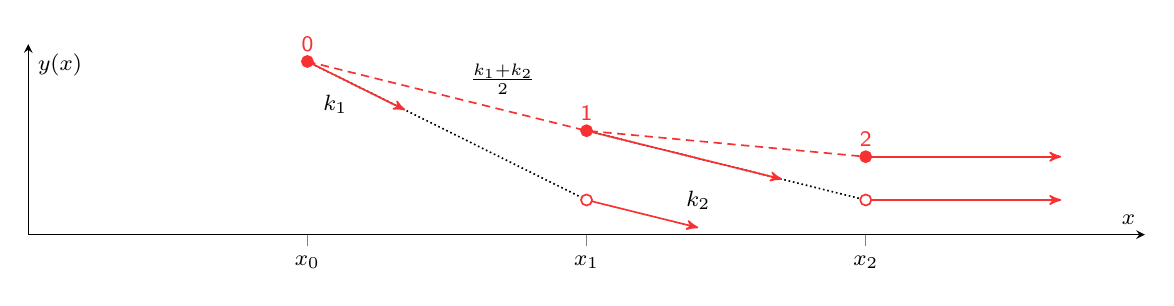
\begin{tikzpicture}
      \begin{axis}[every axis/.append style={font=\footnotesize},
      width=1.3\columnwidth, height=4cm,
      xmin=0,xmax=4,ymin=0,ymax=1.1,
      xtick={1,2,3},ytick={0},
      axis x line=middle,axis y line=middle,
      xlabel=$x$,xticklabels={$x_0$,$x_1$,$x_2$},
      ylabel=$y(x)$,tick align=outside]

      \draw[line,-,black,densely dotted] (axis cs:1,1) -- (axis cs:2,0.2);
      \draw[line,-,black,densely dotted] (axis cs:2,0.6) -- (axis cs:3,0.2);

    \addplot[graph,quiver={u=\thisrow{u},v=\thisrow{v},scale arrows=0.7},-stealth',mark=*,nodes near coords={\coordindex}]
      table {
      x   y     u    v
      1   1     0.5   -0.4
      2   0.6   1 -0.4
      3  0.45   1  0
      };
      \addplot[graph,quiver={u=\thisrow{u},v=\thisrow{v},scale arrows=0.4},-stealth',mark=*,mark options={solid,fill=white}]
      table {
      x   y     u    v
      2   0.2   1   -0.4
      3   0.2   1.75   0
      };
      \addplot[graph,sharp plot,densely dashed]
      table {
      x   y     u    v
      1   1     0.5   -0.5
      2   0.6   1 -0.2
      3  0.45   1  0
      };
      \node[black] at (axis cs:1.1,0.75) {$k_1$};
      \node[black] at (axis cs:2.4,0.20) {$k_2$};
      \node[black] at (axis cs:1.7,0.9) {$\frac{k_1+k_2}{2}$};
%       \node[black] at (axis cs:2.6,0.4) {$k_2$};
      \end{axis}
  \end{tikzpicture}
  \end{columns}
\end{frame}



% \begin{frame}[t,fragile]
% \frametitle{Runge-Kutta methods}
%   Propagate a solution by combining the information of several Euler-style steps (each involving one function evaluation) to match a Taylor series expansion up to some higher order.
%   \vskip1em
%   Euler: $ y_{i+1} = y_i + h f(x_i,y_i) $ with $h = \Delta x$, i.e. $\text{slope} = k_1 = f(x_i,y_i)$.\\
%   \begin{columns}
%     \column{0.5\textwidth}
%     \begin{center}Euler's method\end{center}
%     \begin{tikzpicture}
%       \begin{axis}[every axis/.append style={font=\footnotesize},
%       width=1.3\columnwidth, height=4cm,
%       xmin=0,xmax=4,ymin=0,ymax=4,
%       xtick={1,2,3},ytick={0},
%       axis x line=middle,axis y line=middle,
%       xlabel=$x$,xticklabels={$x_1$,$x_2$,$x_3$},
%       ylabel=$y(x)$,tick align=outside]
% 
%     \addplot[graph,quiver={u=\thisrow{u},v=\thisrow{v},scale arrows=0.4},-stealth']
%       table {
%       x y u v
%       1 1 1 1
%       2 2 1 0.5
%       };
%       \addplot[graph,sharp plot,densely dashed,mark=*,mark options={solid,fill=tuered},mark size=1.7pt,nodes near coords={\coordindex}]
%       table {
%       x y
%       1 1
%       2 2
%       3 2.5
%       };
%     \end{axis}
%   \end{tikzpicture}
%   \column{0.5\textwidth}
%     \begin{center}RK2 method\end{center}
%     \begin{tikzpicture}
%       \begin{axis}[every axis/.append style={font=\footnotesize},
%       width=1.3\columnwidth, height=4cm,
%       xmin=0,xmax=4,ymin=0,ymax=1.1,
%       xtick={1,1.5,2,2.5,3},ytick={0},
%       axis x line=middle,axis y line=middle,
%       xlabel=$x$,xticklabels={$x_0$,$x_\frac{1}{2}$,$x_1$,$x_\frac{3}{2}$,$x_2$},
%       ylabel=$y(x)$,tick align=outside]
% 
%     \addplot[graph,quiver={u=\thisrow{u},v=\thisrow{v},scale arrows=0.4},-stealth',mark=*,nodes near coords={$c_\coordindex$}]
%       table {
%       x   y     u    v
%       1   1     0.5   -0.5
%       2   0.6 1 -0.2
%       3  0.45  1  0
%       };
%       \addplot[graph,quiver={u=\thisrow{u},v=\thisrow{v},scale arrows=0.4},-stealth',mark=*,mark options={solid,fill=white}]
%       table {
%       x   y     u    v
%       1.5 0.5 1   -0.4
%       2.5   0.5 1 -0.15
%       };
%       \addplot[graph,sharp plot,densely dashed]
%       table {
%       x   y     u    v
%       1   1     0.5   -0.5
%       2   0.6 1 -0.2
%       3  0.45  1  0
%       };
%       \node[black] at (axis cs:1.1,0.8) {$k_1$};
%       \node[black] at (axis cs:1.7,0.35) {$k_2$};
%       \node[black] at (axis cs:2.1,0.5) {$k_1$};
%       \node[black] at (axis cs:2.6,0.4) {$k_2$};
%       \end{axis}
%   \end{tikzpicture}
%   \end{columns}
% \end{frame}

\begin{frame}[t,fragile]
  \frametitle{Classical second order Runge-Kutta (RK2) method}
  \footnotesize\selectfont
   This method is also called Heun's method, or improved Euler method:
  \begin{enumerate}
    \item Approximate the slope at $x_i$: $k_1 = f(x_i,y_i)$
    \item Approximate the slope at $x_{i+1}$: $k_2 = f(x_{i+1},y_{i+1})$ where we use Euler's method to approximate $y_{i+1} = y_i + h f(x_i,y_i) = y_i + h k_1$
    \item Perform an Euler step with the average of the slopes: $y_{i+1} = y_i + h\frac{1}{2}(k_1+k_2)$
  \end{enumerate}
  \pause\vskip1em
  In pseudocode:\\
  \tikz{\node[emphblock, text width=0.5\textwidth] {
    \begin{algorithmic}
    \State $x = x_0$, $y = y_0$
    \While {$x < x_\text{end}$}
        \State $x_{i+1} = x_i + h$
        \State $k_1 = f(x_i,y_i)$
        \State $k_2 = f(x_i+h,y_i+h k_1)$
        \State $y_{i+1} = y_i + h \frac{1}{2}\left( k_1 + k_2 \right)$
    \EndWhile \\
    \end{algorithmic} };}
\end{frame}

\begin{frame}
  \frametitle{Runge-Kutta methods --- derivation}
  \footnotesize\selectfont
  \[ \frac{dy}{dx} = f(x,y(x)) \]
  \pause Using Taylor series expansion: $\displaystyle     y_{i+1} = y_i + h \left.\frac{dy}{dx}\right|_i + \left.\frac{h^2}{2}\frac{d^2y}{dx^2}\right|_i + \mathcal{O}{(h^3)} $
  \begin{align*}
    \left.\frac{dy}{dx}\right|_i &= f(x_i,y_i) \equiv f_i \\
    \left.\frac{d^2y}{dx^2}\right|_i &= \left.\frac{d}{dx}f(x,y(x))\right|_i = \left.\frac{\partial f}{\partial x}\right|_i + \left.\frac{\partial f}{\partial y}\right|_i \left.\frac{\partial y}{\partial x}\right|_i = \left.\frac{\partial f}{\partial x}\right|_i + \left.\frac{\partial f}{\partial y}\right|_i f_i \quad \text{(chain rule)}
  \end{align*}
  \pause Substitution gives:
   \begin{align*}
    y_{i+1} &= y_i + h f_i + \frac{h^2}{2} \left( \left.\frac{\partial f}{\partial x}\right|_i +  \left.\frac{\partial f}{\partial y}\right|_i f_i \right) + \mathcal{O}{(h^3)} \\
    y_{i+1} &= y_i + \frac{h}{2} f_i + \frac{h}{2} \left( f_i + h\left.\frac{\partial f}{\partial x}\right|_i + h f_i \left.\frac{\partial f}{\partial y}\right|_i \right) + \mathcal{O}{(h^3)}
  \end{align*}
\end{frame}

{\nologo
\begin{frame}
  \frametitle{Runge-Kutta methods --- derivation}
%   \footnotesize\selectfont
  Note multivariate Taylor expansion:
  \begin{multline*}
    f(x_i+h,y_i+k) = f_i + h \left. \frac{\partial f}{\partial x}\right|_i + k\left. \frac{\partial f}{\partial y}\right|_i + \mathcal{O}{(h^2)} \\
    \Rightarrow \frac{h}{2}\left(f_i + h\left.\frac{\partial f}{\partial x}\right|_i + h f_i \left. \frac{\partial f}{\partial y} \right|_i \right) = \frac{h}{2} f\left(x_i+h,y_i+hf_i\right) + \mathcal{O}{(h^3)}
  \end{multline*}
  Concluding:
  \[
    y_{i+1} = y_i + \frac{h}{2} f_i + \frac{h}{2} f\left(x_i+h,y_i+hf_i\right) + \mathcal{O}{(h^3)}
  \]
  Rewriting:\\
  \tikz{\node[emphblock, text width=0.5\textwidth] {
  \vspace*{-1.5em}
  \begin{align*}
    k_1 &= f\left(x_i,y_i\right) \\
    k_2 &= f\left(x_i+h,y_i+hk_1\right) \\
    \Rightarrow y_{i+1} &= y_i + \frac{h}{2}(k_1 + k_2)
    \end{align*} };}
\end{frame}

\begin{frame}
  \frametitle{Runge-Kutta methods --- derivation}
  \footnotesize\selectfont
  Generalization: {\color<4>{tuealert}$y_{i+1} = y_i + h(b_1 k_1 + b_2 k_2) + \mathcal{O}{(h^3)}$} \\
  with $k_1 = f_i$, $k_2 = f(x_i + c_2 h, y_1 + a_{2,1}h k_1)$\\
  (Note that classical RK2: $b_1 = b_2 = \frac{1}{2}$ and $c_2 = a_{2,1}=1$.) \vskip1em \pause
  Bivariate Taylor expansion:
  \[
    f(x_i+c_2 h, y_i + a_{2,1}h k_1 ) = f_i + c_2 h \left. \frac{\partial f}{\partial x}\right|_i + a_{2,1}hk_1\left. \frac{\partial f}{\partial y}\right|_i + \mathcal{O}{(h^2)}
  \]
\begin{align*}
    y_{i+1} &= y_i + h(b_1 k_1 + b_2 k_2) + \mathcal{O}{(h^3)} \\
    &= y_i + h\left[b_1 f_i + b_2 f(x_i + c_2 h, y_1 + a_{2,1}h k_1)\right] + \mathcal{O}{(h^3)} \\
    &= y_i + h\left[b_1 f_i + b_2 \left\{ f_i + c_2 h \left.\frac{\partial f}{\partial x}\right|_i + a_{2,1} h k_1 \left.\frac{\partial f}{\partial y}\right|_i + \mathcal{O}{(h^2)} \right\}\right] + \mathcal{O}{(h^3)} \\
    &= {\color<4>{tuealert}y_i + h(b_1 + b_2)f_i + h^2b_2\left( c_2 \left.\frac{\partial f}{\partial x}\right|_i + a_{2,1}f_i \left.\frac{\partial f}{\partial y}\right|_i \right) + \mathcal{O}{(h^3)} }
\end{align*} \pause
Comparison with Taylor: 
\[
  {\color<4>{tuealert}y_{i+1} = y_i + h f_i + \frac{h^2}{2}\left( \left. \frac{\partial f}{\partial x}\right|_i + \left. \frac{\partial f}{\partial y}\right|_i f_i \right) + \mathcal{O}{(h^3)}}
\]
Using $b_1+b_2=1$, $c_2b_2=\frac{1}{2}$, $a_{2,1}b_2=\frac{1}{2} \Rightarrow$ 3 eqns and 4 unknowns $\Rightarrow$ multiple possibilities!

\end{frame}
}

\begin{frame}
  \frametitle{Runge-Kutta methods --- derivation}
%   \footnotesize\selectfont
  \begin{align*}
%     y_{i+1} &= y_i + h(b_1 k_1 + b_2 k_2) + \mathcal{O}{(h^3)} \\
    y_{i+1} &= y_i + h(b_1 + b_2)f_i + h^2b_2\left( c_2 \left.\frac{\partial f}{\partial x}\right|_i + a_{2,1}f_i \left.\frac{\partial f}{\partial y}\right|_i \right) + \mathcal{O}{(h^3)} \\
    y_{i+1} &= y_i + h f_i + \frac{h^2}{2}\left( \left. \frac{\partial f}{\partial x}\right|_i + \left. \frac{\partial f}{\partial y}\right|_i f_i \right) + \mathcal{O}{(h^3)}
  \end{align*}
  \vfill
  $\Rightarrow$ 3 eqns and 4 unknowns $\Rightarrow$ multiple possibilities!\vskip1em 
  \begin{enumerate}
    \item Classical RK2: \\
    $b_1 = b_2 = \frac{1}{2}$ and $c_2 = a_{2,1}=1$
    \item Midpoint rule (modified Euler): \\
    $ b_1 = 0$, $b_2 = 1$, $c_2 = a_{2,1} = \frac{1}{2}$\\ 
  \end{enumerate}
  \vfill
\end{frame}


\begin{frame}[t,fragile]
  \frametitle{Second order Runge-Kutta methods}
  \footnotesize\selectfont
%     \rowcolors[]{2}{maincolor!20}{maincolor!10}
    \begin{longtable}{c c}
    \hline
    \begin{minipage}{0.4\textwidth}\centering Classical~RK2 method \\(=~Heun's~method, improved~Euler~method)\end{minipage} & \begin{minipage}{0.4\textwidth}\centering Explicit midpoint rule  (modified~Euler~method)\end{minipage} \\ \hline
    $k_1 = f_i$ & $k_1 = f_i$ \\
    $k_2 = f(x_i + h, y_i + h k_1)$ & $k_2 = f(x_i + \frac{1}{2}h, y_i + \frac{1}{2} h k_1)$ \\
    $y_{i+1} = y_i + \frac{1}{2} h (k_1 + k_2)$ & $y_{i+1} = y_i + h k_2$ \\
    \hline
  \end{longtable}
  \begin{columns}
    \column{0.5\textwidth}
    \begin{tikzpicture}
      \begin{axis}[every axis/.append style={font=\footnotesize},
      width=1.2\columnwidth, height=5.5cm,
      xmin=0,xmax=4,ymin=0,ymax=1.1,
      xtick={1,2,3},ytick={1,0.6,0.45},
      axis x line=middle,axis y line=middle,
      xlabel=$x$,xticklabels={$x_0$,$x_1$,$x_2$},
      ylabel=$y(x)$,yticklabels={$y_0$,$y_1$,$y_2$},tick align=outside]

      \draw[line,-,black,densely dotted] (axis cs:1,1) -- (axis cs:2,0.2);
      \draw[line,-,black,densely dotted] (axis cs:2,0.6) -- (axis cs:3,0.2);

    \addplot[graph,quiver={u=\thisrow{u},v=\thisrow{v},scale arrows=0.7},-stealth',mark=*,nodes near coords={\coordindex}]
      table {
      x   y     u    v
      1   1     0.5   -0.4
      2   0.6   1 -0.4
      3  0.45   1  0
      };
      \addplot[graph,quiver={u=\thisrow{u},v=\thisrow{v},scale arrows=0.4},-stealth',mark=*,mark options={solid,fill=white}]
      table {
      x   y     u    v
      2   0.2   1   -0.4
      3   0.2   1.75   0
      };
      \addplot[graph,sharp plot,densely dashed]
      table {
      x   y     u    v
      1   1     0.5   -0.5
      2   0.6   1 -0.2
      3  0.45   1  0
      };
      \node[black] at (axis cs:1.1,0.75) {$k_1$};
      \node[black] at (axis cs:2.4,0.20) {$k_2$};
      \node[black] at (axis cs:1.7,0.9) {$\frac{k_1+k_2}{2}$};
%       \node[black] at (axis cs:2.6,0.4) {$k_2$};
      \end{axis}
  \end{tikzpicture}
  \column{0.5\textwidth}
  \begin{tikzpicture}
      \begin{axis}[every axis/.append style={font=\footnotesize},
      width=1.2\columnwidth, height=5.5cm,
      xmin=0,xmax=4,ymin=0,ymax=1.1,
      xtick={1,1.5,2,2.5,3},ytick={1,0.6,0.45},
      axis x line=middle,axis y line=middle,
      xlabel=$x$,xticklabels={$x_0$,$x_\frac{1}{2}$,$x_1$,$x_\frac{3}{2}$,$x_2$},
      ylabel=$y(x)$,yticklabels={$y_0$,$y_1$,$y_2$},tick align=outside]

    \draw[line,-,black,densely dotted] (axis cs:1,1) -- (axis cs:1.5,0.5);
    \draw[line,-,black,densely dotted] (axis cs:2,0.6) -- (axis cs:2.5,0.5);
      
    \addplot[graph,quiver={u=\thisrow{u},v=\thisrow{v},scale arrows=0.4},-stealth',mark=*,nodes near coords={\coordindex}]
      table {
      x   y     u    v
      1   1     0.5   -0.5
      2   0.6 1 -0.2
      3  0.45  1  0
      };
      \addplot[graph,quiver={u=\thisrow{u},v=\thisrow{v},scale arrows=0.4},-stealth',mark=*,mark options={solid,fill=white}]
      table {
      x   y     u    v
      1.5 0.5 1   -0.4
      2.5   0.5 1 -0.15
      };
      \addplot[graph,sharp plot,densely dashed]
      table {
      x   y     u    v
      1   1     0.5   -0.5
      2   0.6 1 -0.2
      3  0.45  1  0
      };
      \node[black] at (axis cs:1.1,0.8) {$k_1$};
      \node[black] at (axis cs:1.7,0.35) {$k_2$};
      \node[black] at (axis cs:1.7,0.85) {$k_2$};
%       \node[black] at (axis cs:2.6,0.4) {$k_2$};
      \end{axis}
  \end{tikzpicture}
  \end{columns}
\end{frame}


\begin{frame}[t,fragile]
  \frametitle{Second order Runge-Kutta method --- Example}
  First order reaction in a batch reactor:$\frac{dc}{dt} = -kc$ with $c(t=0) = 1$~\si{\mole\per\cubic\meter}, $k = 1$ \si{s^{-1}}, $t_\text{end} = 2$ \si{\second}.
  \scriptsize\selectfont
  \begin{longtable}{p{0.1\textwidth}p{0.2\textwidth}p{0.25\textwidth}p{0.35\textwidth}}
  \hline
    Time [\si{\second}] & C [\si{\mole\per\cubic\meter}] & $k_1 = hf(x_i,y_i)$ & $k_2 = hf(x_i + \frac{1}{2}h,y_n + \frac{1}{2}k_1)$\\ \hline
    $0$   & $1.00$ & $0.1\cdot(-1\cdot1) = -0.1$& $0.1\cdot(-1\cdot(1-0.5\cdot0.1))=-0.095$\\
    $0.1$   & $1-0.095=0.905$ & $0.1\cdot(-1\cdot0.0905) = -0.0905$& $0.1\cdot(-1\cdot(0.905-0.5\cdot0.0905))=-0.085975$\\
   $\quad \ldots$ & $\quad \quad \ldots$ & $\quad \quad \quad \ldots$ & $\quad \quad \quad \ldots$ \\
   $2$ & $0.1358225$ & $-0.0135822$ & $-0.0129031$ \\
    \hline
  \end{longtable}
 \begin{tikzpicture}
      \begin{axis}[every axis/.append style={font=\footnotesize},
      width=\columnwidth, height=4.5cm,
      xmin=0,xmax=4,ymin=0,ymax=1.1,
      xtick={1,1.5,2,2.5,3},ytick={0},
      axis x line=middle,axis y line=left,
      xlabel=$t$,xticklabels={$t_0$,$t_\frac{1}{2}$,$t_1$,$t_\frac{3}{2}$,$t_2$},
      ylabel=$c(t)$,tick align=outside]

    \addplot[graph,quiver={u=\thisrow{u},v=\thisrow{v},scale arrows=0.4},-stealth',mark=*,nodes near coords={$c_\coordindex$}]
      table {
      x   y     u    v
      1   1     0.5   -0.5
      2   0.6 1 -0.2
      3  0.45  1  0
      };
      \addplot[graph,quiver={u=\thisrow{u},v=\thisrow{v},scale arrows=0.4},-stealth',mark=*,mark options={solid,fill=white}]
      table {
      x   y     u    v
      1.5 0.5 1   -0.4
      2.5   0.5 1 -0.15
      };
      \addplot[graph,sharp plot,densely dashed]
      table {
      x   y     u    v
      1   1     0.5   -0.5
      2   0.6 1 -0.2
      3  0.45  1  0
      };
      \node[black] at (axis cs:1.1,0.8) {$k_1$};
      \node[black] at (axis cs:1.7,0.35) {$k_2$};
      \node[black] at (axis cs:2.1,0.5) {$k_1$};
      \node[black] at (axis cs:2.6,0.4) {$k_2$};
      \end{axis}
  \end{tikzpicture}
\end{frame}

\begin{frame}
  \frametitle{RK2 method --- order of convergence}
  \begin{longtable}{cccc}
    \hline
    $N$ & $\zeta$ & $\frac{\zeta^{}_\text{numerical}-\zeta_\text{analytical}}{\zeta_\text{analytical}}$ & $ r = \frac{\log\left(\frac{\epsilon_i}{\epsilon_{i-1}}\right)}{\log \left( \frac{N_{i-1}}{N_i}\right)} $ \\ \hline
    20  & 0.864178 & \num{5.634E-04} & ---\\
    40  & 0.864548 & \num{1.355E-04} & 2.056\\
    80  & 0.864636 & \num{3.323E-05} & 2.028\\
    160 & 0.864658 & \num{8.229E-06} & 2.014\\
    320 & 0.864663 & \num{2.048E-06} & 2.007\\
    \hline
  \end{longtable}
  \pause
  $ \Rightarrow$ RK2 is a second order method. Doubling the number of cells reduces the error by a factor 4! \\
  \vskip1em
  Can we do even better?
\end{frame}

\subsection{RK4 method}
{\nologo
\begin{frame}
  \frametitle{RK4 method (classical fourth order Runge-Kutta method)}
  \vskip1em
  \centering
  \begin{tikzpicture}[scale=0.8,xscale=1.3]
    \draw[line,-,densely dashed] (0,4)  .. node [fdot,very near start,solid] (k1) {} node [fdot,midway,above=9pt,solid,fill=white](k2) {} node [fdot,midway,below=9pt,solid,fill=white](k3) {}controls(2,1) and (6,0) .. node [fdot,pos=0.8,solid] (k4) {} (8,0); 
    \draw[line,ultra thick] ($ (k1) +(0.45,-0.5) $) -- ($ (k1) -(0.45,-0.5) $);
    \node[below=2pt] at (k1) {$y_i$}; 
    \draw[line,ultra thick] ($ (k4) +(0.75,-0.127) $) -- ($ (k4) -(0.75,-0.127) $);
    \node[below=2pt] at (k4) {$y_{i+1}$}; 
    \draw[line,ultra thick] ($ (k2) +(0.6,-0.25) $) -- ($ (k2) -(0.6,-0.25) $);
    \draw[line,ultra thick] ($ (k3) +(0.6,-0.25) $) -- ($ (k3) -(0.6,-0.25) $);
    \node[above=3pt] at (k1) {1};
    \node[above=3pt] at (k2) {2};
    \node[below=3pt] at (k3) {3};
    \node[above=3pt] at (k4) {4};
  \end{tikzpicture} 
  \vspace*{-1cm}

  \begin{align*}
    k_1 &= f(x_i, y_i) \\
    k_2 &= f(x_i+\frac{1}{2}h, y_i + \frac{1}{2}hk_1) \\
    k_3 &= f(x_i + \frac{1}{2}h,y_i + \frac{1}{2}hk_2) \\
    k_4 &= f(x_i + h, y_i + hk_3) \\
    y_{i+1} &= y_i + h\left(\frac{1}{6}k_1 + \frac{1}{3}\left(k_2 + k_3\right) + \frac{1}{6}k_4\right)
  \end{align*}
\end{frame}
}


\begin{frame}
  \frametitle{RK4 method --- order of convergence}
  \begin{longtable}{cccc}
    \hline
    $N$ & $\zeta$ & $\frac{\zeta^{}_\text{numerical}-\zeta_\text{analytical}}{\zeta_\text{analytical}}$ & $ r = \frac{\log\left(\frac{\epsilon_i}{\epsilon_{i-1}}\right)}{\log \left( \frac{N_{i-1}}{N_i}\right)} $ \\ \hline
    20  & 0.864664472 & \num{2.836E-07} & ---\\
    40  & 0.864664702 & \num{1.700E-08} & 4.060\\
    80  & 0.864664716 & \num{1.040E-09} & 4.030\\
    160 & 0.864664717 & \num{6.435E-11} & 4.015\\
    320 & 0.864664717 & \num{4.001E-12} & 4.007\\
    \hline
  \end{longtable}
  \pause
  $ \Rightarrow$ RK4 is a fourth order method: Doubling the number of cells reduces the error by a factor 16! \\
  \vskip1em
  Can we do even better?
\end{frame}

\section{Step size control}
\againframe<2>{contents_ode1}
\subsection*{Adaptive step size}
\begin{frame}
  \frametitle{Adaptive step size control}
  The step size (be it either position, time or both (PDEs)) cannot be decreased indefinitely to favour a higher accuracy, since each additional grid point causes additional computation time. It may be wise to adapt the step size according to the computation requirements. \vskip1em
  Globally two different approaches can be used:
  \begin{enumerate}
    \item Step doubling: compare solutions when taking one full step or two consecutive halve steps
    \item Embedded methods: Compare solutions when using two approximations of different order
  \end{enumerate}
\end{frame}

\begin{frame}
  \frametitle{Adaptive step size control: step doubling}
    \begin{tikzpicture}[scale=5]
      \node[] at (1,0.3){};
      \node[] at (1,-0.3){};
      \node[fdot] (t0)  at (0   , 0) {};
      \node<3->[fdot] (t05) at (0.5 , 0) {};
      \node[fdot] (t1)  at (1   , 0) {};
      \node<3->[fdot] (t15) at (1.5 , 0) {};
      \node[fdot] (t2)  at (2   , 0) {};
      \node[above=13pt]  at (t0) {$t$};
      \node[above=13pt]  at (t1) {$t+\Delta t$};
      \node[above=13pt]  at (t2) {$t+2\Delta t$};
            
      \draw[gridline] (t0) -- (t1) -- (t2);
      \draw<2->[line,draw=tuered] (t0) .. node [midway,above] (dt1) {$\Delta t$} controls (0.25,0.2) and (0.75,0.2) .. (t1);
      \draw<2->[line,draw=tuered] (t1) .. node [midway,above] (dt2) {$\Delta t$} controls (1.25,0.2) and (1.75,0.2) .. (t2);
      
      \draw<3->[line,draw=tuelblue] (t0) .. node [midway,below] (dt05) {$\frac{\Delta t}{2}$} controls (0.125,-0.15) and (0.375,-0.15) .. (t05);
      \draw<3->[line,draw=tuelblue] (t05) .. node [midway,below] (dt15) {$\frac{\Delta t}{2}$} controls (0.625,-0.15) and (0.875,-0.15) .. (t1);
      \draw<3->[line,draw=tuelblue] (t1) .. node [midway,below] (dt05) {$\frac{\Delta t}{2}$} controls (1.125,-0.15) and (1.375,-0.15) .. (t15);
      \draw<3->[line,draw=tuelblue] (t15) .. node [midway,below] (dt15) {$\frac{\Delta t}{2}$} controls (1.625,-0.15) and (1.875,-0.15) .. (t2);
      
      \node<2->[above=3pt,color=tuered]  at (t1) {$y_1$};
      \node<3->[below=3pt,color=tuelblue]  at (t1) {$y_2$};
%       \node[above=3pt,color=tuered]  at (t2) {$y_1$};
%       \node[below=3pt,color=tuelblue]  at (t2) {$y_2$};
            

%       \draw[line] (t1) .. node [midway,above] (dt2) {$\Delta t$} controls (1.25,0.2) and (1.75,0.2) .. (t2);

%       \draw[line,densely dashed] (0.1,0.05) -- node[midway,above] {``Marching''} (0.9,0.05);
    \end{tikzpicture}\begin{itemize}
  \item<2-> \color{tuered} RK4 with one large step of $h$: $ y_{i+1} = y_1 + ch^5 + \mathcal{O}{(h^6)} $
  \item<3-> \color{tuelblue} RK4 with two steps of $\frac{1}{2}h$: $ y_{i+1} = y_2 + 2c(\frac{1}{2}h)^5 + \mathcal{O}{(h^6)} $
\end{itemize}
\end{frame}

\begin{frame}
  \frametitle{Adaptive step size control: step doubling}
\begin{itemize}
  \item Estimation of truncation error by comparing $y_1$ and $y_2$:\\
  $\Delta = y_2 - y_1$
  \item If $\Delta$ too large, reduce step size for accuracy
  \item If $\Delta$ too small, increase step size for efficiency.
  \item Ignoring higher order terms and solving for $c$:
  $ \Delta = \frac{15}{16}ch^5 \Rightarrow ch^5 = \frac{16}{15} \Delta \Rightarrow y_{i+1} = y_2 + \frac{\Delta}{15} + \mathcal{O}{(h^6)}$ \\ (local Richardson extrapolation)
\end{itemize}
  Note that when we specify a tolerance \emph{tol}, we can estimate the maximum allowable step size as:
  $ h_\text{new} = \alpha h_\text{old} \abs{\frac{\text{tol}}{\Delta}}^{\frac{1}{5}}$ with $\alpha$ a safety factor (typically $\alpha = 0.9$).
\end{frame}

\begin{frame}
  \frametitle{Adaptive step size control: embedded methods}
  Use a special fourth and a fifth order Runge Kutta method to approximate $y_{i+1}$
  \begin{itemize}
    \item The fourth order method is special because we want to use the same positions for the evaluation for computational efficiency.
    \item RK45 is the preferred method (minimum number of function evaluations) (used in Python as \lstinline$scipy.integrate.solve_ivp$).
  \end{itemize}
\end{frame}

\section{Solving ODEs in Python}
\againframe<2>{contents_ode1}
\subsection*{Solving ODEs in Python}
\begin{frame}
  \frametitle{Solving ODEs in Python}
  Python, with the help of the SciPy library, provides convenient procedures to solve (systems of) ODEs automatically.
  \vskip1em
  The procedure is as follows:
  \begin{enumerate}
    \item Create a function that specifies the ODE(s). Specifically, this function returns the $\frac{dy}{dx}$ value (vector).
    \item Initialise solver variables and settings (e.g., step size, initial conditions, tolerance), in a separate script or within the main script.
    \item Call the ODE solver function, passing the ODE function created in step 1 as an argument.
    \begin{itemize}
      \item The ODE solver will return an object containing the independent variable vector and a solution vector (matrix for systems of ODEs).
    \end{itemize}
  \end{enumerate}
\end{frame}

\begin{frame}[fragile]
  \frametitle{Solving ODEs in Python: example 1}
  We solve the system: $\displaystyle \frac{dx}{dt} = -k_1 x + k_2, k_1 = 0.2, k_2=2.5$
  \begin{itemize}
    \item Define a function that represents the equation:
    \begin{lstlisting}[language=Python]
from scipy.integrate import solve_ivp

def my_eqn(t, x):
    return -0.2*x + 2.5
    \end{lstlisting}
    \item Solve with a call to \lstinline|solve_ivp(function, timespan, initial_condition)|:
    \begin{lstlisting}[language=Python]
sol = solve_ivp(my_eqn, [0, 40], [0], t_eval=[i for i in range(41)])
    \end{lstlisting}
    \item To plot the solution:
    \begin{lstlisting}[language=Python]
import matplotlib.pyplot as plt

plt.plot(sol.t, sol.y[0])
plt.xlabel('t')
plt.ylabel('x')
plt.grid()
plt.show()
    \end{lstlisting}
  \end{itemize}
\vfill
\end{frame}


\begin{frame}[fragile]
  \frametitle{Solving ODEs in Python: example 2}
  We solve the system: $\displaystyle \frac{dx}{dt} = \begin{cases}
    -\frac{k_1}{x^2} \quad\ \quad t \leq 10\\
    \frac{k_2}{x} - \frac{k_1}{x^2} \quad  t > 10\\
 \end{cases}\, \text{with }\, k_1 = 0.5,\, k_2 = 1,\, x(0) = 2$
 \vspace*{0ex}
  \begin{block}{Create an ODE function in Python}
    \begin{lstlisting}[language=Python,basicstyle=\tiny]
def my_eqn_function(t, x):
    k1 = 0.5
    k2 = 1
    if t <= 10:
        dxdt = -k1 / x**2
    else:
        dxdt = k2 / x - k1 / x**2
    return dxdt
\end{lstlisting}
  \end{block}
  \pause
  \begin{block}{Create a solution script in Python}
    \begin{lstlisting}[language=Python,basicstyle=\tiny]
from scipy.integrate import solve_ivp

x_init = [2]  # Initial condition
t_span = [0, 20]  # Time span

sol = solve_ivp(my_eqn_function, t_span, x_init, t_eval=[i for i in range(21)], rtol=1e-8, atol=1e-8)

# Use sol.t and sol.y to access the solution
\end{lstlisting}
  \end{block}
\vfill
\end{frame}


{\nologo
\begin{frame}[fragile]
  \frametitle{Solving ODEs in Python: example 2}
  Plot the solution:
  \begin{lstlisting}
plt.plot(t,x,'-x')
  \end{lstlisting}
  \pause
  \begin{center}
    \begin{tikzpicture}
      \begin{axis}[%every axis/.append style={font=\footnotesize},
        width=\textwidth, height=6cm,     % size of the image
        grid = major,grid style={dashed, gray!30},
        axis background/.style={fill=white},
        axis x line=middle,axis y line=middle,ylabel=$x$,xlabel=$t$]

        \addplot[graph,mark=x] table []{data/ODE_matlabsolve_single2.dat};  
        \addlegendentry{$x_1$}
      %  \addlegendentry{$x_2$}
      \end{axis}
    \end{tikzpicture}
  \end{center}
  Note the refinement in regions where large changes occur.
\end{frame}
}

\begin{frame}[fragile]
  \frametitle{Solving ODEs in Python: example}
  A few notes on working with \lstinline$solve_ivp$ and other solvers in Python. If we want to give additional arguments (e.g. \lstinline$k1$ and \lstinline$k2$) to our ODE function, we can pass them using the \lstinline$args$ parameter:
  \begin{lstlisting}[language=Python]
def my_eqn(t, x, k1, k2):
    # ... function body ...
\end{lstlisting}
  The additional arguments can now be set in the solver script by using the \lstinline$args$ parameter:
  \begin{lstlisting}[language=Python]
sol = solve_ivp(my_eqn, t_span, x_init, args=(k1, k2))
\end{lstlisting}
  \pause
  \begin{itemize}
    \item Of course, in the solver script, the variables do not have to be called \lstinline$k1$ and \lstinline$k2$:
      \begin{lstlisting}[language=Python]
sol = solve_ivp(my_eqn, t_span, x_init, args=(q, u))
\end{lstlisting}
    \item These variables may be of any type (lists, arrays, dictionaries). Especially a dictionary is useful to carry many values in 1 variable.
  \end{itemize}
\end{frame}

\begin{frame}[fragile]
  \frametitle{Solving systems of ODEs in Python: example}
  You have noticed that the step size in $t$ varied. This is because we have given just the begin and end times of our time span:
  \begin{lstlisting}[language=Python]
t_span = [0, 10]
\end{lstlisting}
  \pause
  You can also solve at specific steps, by supplying all steps explicitly, e.g.:
  \begin{lstlisting}[language=Python]
t_eval = np.linspace(0, 10, 101)
sol = solve_ivp(my_eqn, t_span, x_init, t_eval=t_eval)
\end{lstlisting}
  This example provides 101 explicit time steps between 0 and 10 seconds.
  \vskip1em
  Note that the results are interpolated to these data points afterwards; you do not influence the efficiency and accuracy of the solver algorithm this way!
  \vfill
\end{frame}

\title{Ordinary differential equations 2}
\subtitle{Implicit methods, systems of ODEs and boundary value problems}
\lecture{ODE 2}{ode2}
\part{Ordinary differential equations II - Implicit methods and systems of ODEs}
\section{Introduction}
\subsection*{General}
\begin{frame}[label=contents_ode2]
  \frametitle{Today's outline}
  \mode<beamer>{
    \only<1>{\tableofcontents}
  }
  \only<2>{\tableofcontents[currentsection,currentsubsection]}
\end{frame}

\subsection{Backward Euler}
\begin{frame}
  \frametitle{Problems with Euler's method: instability}
  Consider the ODE:
  \[
    \frac{dy}{dx} = f(x,y(x)) \qquad \text{with} \qquad y(x=0) = y_0
  \]
  \vskip1em
  \pause
  First order approximation of derivative: $\frac{dy}{dx} = \frac{y_{i+1}-y_i}{\Delta x}$. 
  \vskip1em
  Where to evaluate the function $f$?
  \vskip1em
  \pause
  \begin{enumerate}
    \item Evaluation at $x_i$:  Explicit Euler method (forward Euler)
    \item Evaluation at $x_{i+1}$: Implicit Euler method (backward Euler)
  \end{enumerate}
\end{frame}

\begin{frame}
  \frametitle{Problems with Euler's method: instability -- forward Euler}
  Explicit Euler method (forward Euler):
    \begin{itemize}
      \item Use values at $x_i$: \\ $\frac{y_{i+1}-y_i}{\Delta x} = f(x_i,y_i) \Rightarrow y_{i+1} = y_i + h f(x_i,y_i)$. 
      \item This is an explicit equation for $y_{i+1}$ in terms of $y_i$.
      \item It can give instabilities with large function values.
    \end{itemize}
    \pause \vskip1em
    Consider the first order batch reactor: 
    \[
      \frac{dc}{dt} = -kc \Rightarrow c_{i+1} = c_i - k{\color{tuered}c_i}\Delta t \Rightarrow \frac{c_{i+1}}{c_i} = 1-k\Delta t
    \]
    \pause
    It follows that unphysical results are obtained for $k\Delta t \geq 1$!! \vskip1em
    \begin{block}{Stability requirement}
      \centering $k \Delta t < 1$\\ (but probably accuracy requirements are more stringent here!)
    \end{block}
\end{frame}
\begin{frame}
  \frametitle{Problems with Euler's method: instability -- backward Euler}
  Implicit Euler method (backward Euler):
    \begin{itemize}
      \item Use values at $x_{i+1}$: $\frac{y_{i+1}-y_i}{\Delta x} = f(x_{i+1},y_{i+1}) \Rightarrow y_{i+1} = y_i + h f(x_{i+1},y_{i+1})$. 
      \item This is an implicit equation for $y_{i+1}$, because it also depends on terms of $y_{i+1}$.
    \end{itemize}
    \pause \vskip1em
    Consider the first order batch reactor: 
    \[
      \frac{dc}{dt} = -kc \Rightarrow c_{i+1} = c_i - k{\color{tuered}c_{i+1}}\Delta t \Rightarrow \frac{c_{i+1}}{c_i} = \frac{1}{1+k\Delta t}
    \]
    \pause
    This equation does never give unphysical results!\\
    The implicit Euler method is \emph{unconditionally stable} \\
    (but maybe not very accurate or efficient).
\end{frame}


\begin{frame}
  \frametitle{Semi-implicit Euler method}
  \footnotesize\selectfont
  Usually $f$ is a non-linear function of $y$, so that linearization is required (recall Newton's method).
  
  \begin{align*}
    \frac{dy}{dx} &= f(y) \Rightarrow y_{i+1} = y_i + h f (y_{i+1}) \quad \text{using} \quad f(y_{i+1}) = f(y_i) + \left.\frac{df}{dy}\right|_i(y_{i+1}-y_i) + \ldots \\
  &\Rightarrow y_{i+1} =  y_i + h \left[ f(y_i) + \left.\frac{df}{dy}\right|_i (y_{i+1}-y_i) \right] \\ 
  &\Rightarrow \left(1-h\left.\frac{df}{dy}\right|_i \right)y_{i+1} = \left(1-h\left.\frac{df}{dy}\right|_i\right)y_i + h f(y_i) 
  \end{align*}
  
  \tikz{\node[emphblock,text width=\textwidth] {$\displaystyle \Rightarrow y_{i+1} = y_i + h \left( 1 - h \left.\frac{df}{dy}\right|_i \right)^{-1} f(y_i) $};}
  \pause
  For the case that $f(x,y(x))$ we could add the variable $x$ as an additional variable $y_{n+1}=x$. Or add one fully implicit Euler step (which avoids the computation of $\frac{\partial f}{\partial x}$): \vspace*{-1em}
  \[
    y_{i+1} = y_i + h f(x_{i+1},y_{i+1}) \Rightarrow y_{i+1} = y_i + h \left(1-h\left.\frac{df}{dy}\right|_i \right)^{-1} f(x_{i+1},y_i)
  \]
\end{frame}

\begin{frame}
  \frametitle{Semi-implicit Euler method - example}
  Second order reaction in a batch reactor:\\
  $\frac{dc}{dt} = -kc^2$ with $c_0 = 1$~\si{\mole\per\cubic\meter}, $k = 1$ \si{\cubic\meter\per\mole\per\second}, $t_\text{end} = 2$ \si{\second} \\
  Analytical solution: $c(t) = \frac{c_0}{1+kc_0t}$
  \vskip1em \pause  
  Define $f = -kc^2$, then $\frac{df}{dc} = -2kc \Rightarrow c_{i+1} = c_i - \frac{hkc_i^2}{1+2hkc_i}$.
  \pause
    \begin{longtable}{cccc}
    \hline
    $N$ & $\zeta$ & $\frac{\zeta^{}_\text{numerical}-\zeta_\text{analytical}}{\zeta_\text{analytical}}$ & $ r = \frac{\log\left(\frac{\epsilon_i}{\epsilon_{i-1}}\right)}{\log \left( \frac{N_{i-1}}{N_i}\right)} $ \\ \hline
    20  & 0.654066262 & \num{1.89E-002} & ---\\
    40  & 0.660462687 & \num{9.31E-003} & 1.02220\\
    80  & 0.663589561 & \num{4.62E-003} & 1.01162\\
    160 & 0.665134433 & \num{2.30E-003} & 1.00594\\
    320 & 0.665902142 & \num{1.15E-003} & 1.00300\\
    \hline
  \end{longtable}
\end{frame}

\subsection{Implicit midpoint method}
\begin{frame}
  \frametitle{Second order implicit method: Implicit midpoint method}
  \footnotesize\selectfont
\begin{longtable}{c c}
    \hline
    \begin{minipage}{0.4\textwidth}\centering Implicit midpoint rule \\(second order)\end{minipage} & \begin{minipage}{0.4\textwidth}\centering Explicit midpoint rule  (modified~Euler~method)\end{minipage} \\ \hline
    $y_{i+1} = y_i + hf\left(x_i + \frac{1}{2}h, {\color{tuered}\frac{1}{2}(y_i + y_{i+1})}\right)$  & $y_{i+1} = y_i + hf(x_i + \frac{1}{2}h, {\color{tuered}y_i + \frac{1}{2} h k_1})$ \\
    \hline
  \end{longtable}
  in case $f(y)$ then:
  \[
    f\left(\frac{1}{2}(y_i+y_{i+1})\right) = f_i + \left.\frac{df}{dy}\right|_i \left( \frac{1}{2}(y_i + y_{i+1})-y_i\right) = f_i + \frac{1}{2}\left.\frac{df}{dy}\right|_i(y_{i+1}-y_i)
  \]
  \pause
  Implicit midpoint rule reduces to: 
  \begin{align*}
    y_{i+1} &= y_i + h f_i + \frac{h}{2}\left.\frac{df}{dy}\right|_i(y_{i+1}-y_i)\\
    &\Rightarrow \left(1 - \frac{h}{2} \left.\frac{df}{dy}\right|_i\right)y_{i+1} = \left(1 - \frac{h}{2} \left.\frac{df}{dy}\right|_i\right)y_i + h f_i
  \end{align*}
  \tikz{\node[emphblock,text width=0.7\textwidth] {
    $ \displaystyle \Rightarrow y_{i+1} = y_i + h \left( 1 - \frac{h}{2} \left.\frac{df}{dy}\right|_i\right)^{-1} f_i$
    };}
\end{frame}

\begin{frame}
  \frametitle{Implicit midpoint method --- example}
  Second order reaction in a batch reactor: \\
  $\frac{dc}{dt} = -kc^2$ with $c_0 = 1$~\si{\mole\per\cubic\meter}, $k = 1$ \si{\cubic\meter\per\mole\per\second}, $t_\text{end} = 2$ \si{\second} (Analytical solution: $c(t) = \frac{c_0}{1+kc_0t}$). 
  \vskip1em \pause  
  Define $f = -kc^2$, then $\frac{df}{dc} = -2kc$.\vskip1em \pause
  Substitution: 
  \begin{align*}
    c_{i+1} &= c_i + h \left(1-\frac{h}{2} \cdot (-2kc_i)\right)^{-1} \cdot(-kc^2_i) \\
	    &= c_i - \frac{hkc_i^2}{1+hkc_i} = \frac{c_i + h k c_i^2 - h k c_i^2 }{1+hkc_i} \Rightarrow c_{i+1} = \frac{c_i}{1+hkc_i}
  \end{align*}
  
  \pause
  You will find that this method is exact for all step sizes $h$ because of the quadratic source term!
\end{frame}

\begin{frame}
  \frametitle{Implicit midpoint method --- example}
  {\color{tuealert}Second order} reaction in a batch reactor:\\
  $\frac{dc}{dt} = -kc^2$ with $c_0 = 1$~\si{\mole\per\cubic\meter}, $k = 1$ \si{\cubic\meter\per\mole\per\second}, $t_\text{end} = 2$ \si{\second}\\
  Analytical solution: $c(t) = \frac{c_0}{1+kc_0t}$
  \[
    c_{i+1} = \frac{c_i}{1+hkc_i}
  \]
  \pause  
  \begin{longtable}{cccc}
    \hline
    $N$ & $\zeta$ & $\frac{\zeta^{}_\text{numerical}-\zeta_\text{analytical}}{\zeta_\text{analytical}}$ & $ r = \frac{\log\left(\frac{\epsilon_i}{\epsilon_{i-1}}\right)}{\log \left( \frac{N_{i-1}}{N_i}\right)} $ \\ \hline
    20  & 0.6666666667 & \num{1.665E-016} & ---\\
    40  & 0.6666666667 & \num{0} & ---\\
    80  & 0.6666666667 & \num{0} & ---\\
    160 & 0.6666666667 & \num{0} & ---\\
    320 & 0.6666666667 & \num{0} & ---\\
    \hline
  \end{longtable}
\end{frame}

\begin{frame}
  \frametitle{Implicit midpoint method --- example}
  {\color{tuealert}Third order} reaction in a batch reactor: $\frac{dc}{dt} = -kc^3$\\
  Analytical solution: $c(t) = \frac{c_0}{\sqrt{1+2kc_0^2t}}$
  \[
    c_{i+1} = c_i - \frac{hkc_i^3}{1+\frac{3}{2}hkc_i^2}
  \]
  \pause  
  \begin{longtable}{cccc}
    \hline
    $N$ & $\zeta$ & $\frac{\zeta^{}_\text{numerical}-\zeta_\text{analytical}}{\zeta_\text{analytical}}$ & $ r = \frac{\log\left(\frac{\epsilon_i}{\epsilon_{i-1}}\right)}{\log \left( \frac{N_{i-1}}{N_i}\right)} $ \\ \hline
    20  & 0.5526916174 & \num{1.71E-004} & ---\\
    40  & 0.5527633731 & \num{4.17E-005} & 2.041\\
    80  & 0.5527807304 & \num{1.03E-005} & 2.021\\
    160 & 0.5527849965 & \num{2.55E-006} & 2.011\\
    320 & 0.5527860538 & \num{6.34E-007} & 2.005\\
    \hline
  \end{longtable}
\end{frame}

\section{Systems of ODEs}
\againframe<2>{contents_ode2}
\subsection{Solution methods for systems of ODEs}
\begin{frame}
  \frametitle{Systems of ODEs}
  A system of ODEs is specified using vector notation:
  \[
    \frac{d\vec{y}}{dx} = \vec{f}(x,\vec{y}(x))
  \]
  for
  \begin{multline*}
    \frac{dy_1}{dx} = f_1(x,y_1(x),y_2(x)) \quad \text{or} \quad f_1(x,y_1,y_2)\\
    \frac{dy_2}{dx} = f_2(x,y_1(x),y_2(x)) \quad \text{or} \quad f_2(x,y_1,y_2)\\
  \end{multline*}
  \pause
  \tikz{\node[emphblock,text width=\textwidth] {The solution techniques discussed before can also be used to solve systems of equations.};}
\end{frame}

\begin{frame}
  \frametitle{Systems of ODEs: Explicit methods}
  \begin{block}{Forward Euler method}
    $ \displaystyle  \vec{y}_{i+1} = \vec{y}_i + h \vec{f}(x_i,\vec{y}_i) $
  \end{block}
  \begin{block}{Improved Euler method (classical RK2)}
    $\displaystyle \vec{y}_{i+1} = \vec{y}_i + \frac{h}{2}(\vec{k}_1+\vec{k}_2)$
    \quad using \quad \begin{minipage}{0.4\textwidth}
      $\displaystyle \vec{k}_1 = \vec{f}(x_i,\vec{y}_i)$\\
      $\displaystyle \vec{k}_2 = \vec{f}(x_i+h,\vec{y}_i+h\vec{k}_1)$
    \end{minipage}
  \end{block}  
  \begin{block}{Modified Euler method (midpoint rule)}
    $\displaystyle \vec{y}_{i+1} = \vec{y}_i + h\vec{k}_2$
    \quad using \quad \begin{minipage}{0.4\textwidth}
      $\displaystyle \vec{k}_1 = \vec{f}(x_i,\vec{y}_i)$\\
      $\displaystyle \vec{k}_2 = \vec{f}(x_i+\frac{h}{2},\vec{y}_i+\frac{h}{2}\vec{k}_1)$
    \end{minipage}
  \end{block}   
\end{frame}

\begin{frame}
  \frametitle{Systems of ODEs: Explicit methods}
  \begin{block}{Classical fourth order Runge-Kutta method (RK4)}
    $\displaystyle \vec{y}_{i+1} = \vec{y}_i + h\left(\frac{\vec{k}_1}{6}+\frac{1}{3}\left( \vec{k}_2 + \vec{k}_3\right) + \frac{\vec{k}_4}{6} \right)$
    \\ \vskip2em
\quad using \quad \begin{minipage}{0.4\textwidth}
      $\displaystyle \vec{k}_1 = \vec{f}(x_i,\vec{y}_i)$\\ \vskip1ex
      $\displaystyle \vec{k}_2 = \vec{f}(x_i+\frac{h}{2},\vec{y}_i+\frac{h}{2}\vec{k}_1)$ \\ \vskip1ex
      $\displaystyle \vec{k}_3 = \vec{f}(x_i+\frac{h}{2},\vec{y}_i+\frac{h}{2}\vec{k}_2)$ \\ \vskip1ex
      $\displaystyle \vec{k}_4 = \vec{f}(x_i+h,\vec{y}_i+h\vec{k}_3)$ \\ \vskip1ex
    \end{minipage}
%     \end{center}
  \end{block}  
\end{frame}

\subsection{Solving systems of ODEs in Python}
\begin{frame}
  \frametitle{Solving systems of ODEs in Python}
  Solving systems of ODEs in Python follows a similar process to Matlab but leverages the SciPy library:
  \vspace*{1em}
  \begin{enumerate}
    \item Create a function that specifies the ODEs. This function returns the $\frac{d\vec{y}}{dx}$ vector.
    \item Initialize solver variables and settings (e.g. step size, initial conditions, tolerance) within your Python script. Initial conditions and tolerances should be given per-equation, i.e. as a list or array.
    \item Call the ODE solver function from the SciPy library, passing the ODE function described in point 1 as an argument.
    \begin{itemize}
      \item The ODE solver will return an object that contains the solution arrays for each dependent variable.
    \end{itemize}
  \end{enumerate}
\end{frame}

\begin{frame}[fragile]
  \frametitle{Solving systems of ODEs in Python: example}
  We solve the system: $\displaystyle \frac{dx_1}{dt} = -x_1 - x_2, \quad  \frac{dx_2}{dt} = x_1 - 2x_2 $
  \begin{block}{Create an ODE function}
    \begin{lstlisting}[language=Python]
from scipy.integrate import solve_ivp

def my_ode_function(t, x):
    dxdt = [-x[0] - x[1], x[0] - 2*x[1]]
    return dxdt
    \end{lstlisting}
  \end{block}
  \pause
  \begin{block}{Create a solution script}
    \begin{lstlisting}[language=Python]
x_init = [0, 1]        # Initial conditions
t_span = [0, 10]       # Time span
sol = solve_ivp(my_ode_function, t_span, x_init, rtol=1e-4, atol=[1e-4, 1e-4])

# The solution can be accessed as sol.t (time points) and sol.y (solutions at each time point)
    \end{lstlisting}
  \end{block}
\vfill
\end{frame}


{\nologo
\begin{frame}[fragile]
  \frametitle{Solving systems of ODEs in Python: example}
  Plot the solution using `matplotlib`:
  \begin{lstlisting}[language=Python]
plt.plot(sol.t, sol.y[0], 'r-x', label='x1')
plt.plot(sol.t, sol.y[1], 'b-o', label='x2')
plt.xlabel('t'); plt.ylabel('x'); plt.legend(); plt.grid(); plt.show()
  \end{lstlisting}
  \pause
  \begin{center}
    \begin{tikzpicture}
      \begin{axis}[%every axis/.append style={font=\footnotesize},
        width=\textwidth, height=6.5cm,     % size of the image
        grid = major,grid style={dashed, gray!30},
        axis background/.style={fill=white},
        axis x line=middle,axis y line=middle,ylabel=$x$,xlabel=$t$]

        \addplot[graph,mark=x] table []{data/ODE_matlabsolve1.dat};  \addlegendentry{$x_1$}
        \addplot[graph,mark=o,draw=tueblue,mark options={fill=white}] table []{data/ODE_matlabsolve2.dat};  \addlegendentry{$x_2$}
      \end{axis}
    \end{tikzpicture}
  \end{center}
\end{frame}
}

\begin{frame}[fragile]
  \frametitle{Solving systems of ODEs in Python: repeated notes}
  A few notes on working with `solve\_ivp` and other SciPy solvers. If we want to give additional arguments (e.g. `a`, `b`, and `c`) to our ODE function, we can list them in the function signature:
  \begin{lstlisting}[language=Python]
def my_ode(t, x, a, b, c):
  \end{lstlisting}
  The additional arguments can now be set in the solution script by passing them using the `args` parameter:
  \begin{lstlisting}[language=Python]
sol = solve_ivp(my_ode, t_span, x_init, args=(a, b, c))
  \end{lstlisting}
  \pause
  \begin{itemize}
    \item Of course, in the solution script, the variables do not need to be called `a`, `b`, and `c`. They could be named anything:
      \begin{lstlisting}[language=Python]
sol = solve_ivp(my_ode, t_span, x_init, args=(k1, phi, V))
      \end{lstlisting}
    \item These variables can be of any type (lists, arrays, dictionaries). Especially a dictionary can be useful to carry many values in one variable.
    \item Python inherently supports functions with more arguments than the default `(t, x)` required by `solve\_ivp`, so there is no need for an alternative approach as in MATLAB.
  \end{itemize}
\end{frame}


\begin{frame}[fragile]
  \frametitle{Solving systems of ODEs in Python: example}
  You may have noticed that the step size in \( t \) varied. This is because we have given the begin and end times of our time span, and \texttt{solve\_ivp} uses adaptive step size for efficiency:
  \begin{lstlisting}[language=Python]
t_span = [0, 10]
  \end{lstlisting}
  \pause
  You can also retrieve the solution at specific steps, by supplying all steps explicitly as an array, e.g.:
  \begin{lstlisting}[language=Python]
t_eval = np.linspace(0, 10, 101)
  \end{lstlisting}
  This example provides 101 explicit time steps between 0 and 10 seconds.
  \vskip1em
  Note that this is an interpolated result. The solver uses, in the background, still the adaptive step size functionality!
  \vfill
\end{frame}

\subsection{Stiff systems of ODEs}
\begin{frame}
  \frametitle{Systems of ODEs: Implicit methods}
  \begin{block}{Backward Euler method}
    $ \displaystyle  \vec{y}_{i+1} = \vec{y}_i + h \left(\vec{I} - h\left. \frac{d\vec{f}}{d\vec{y}}\right|_i \right)^{-1}\vec{f}(\vec{y}_i)$
  \end{block}
  \begin{block}{Implicit midpoint method}
    $ \displaystyle  \vec{y}_{i+1} = \vec{y}_i + h \left(\vec{I} - \frac{h}{2}\left. \frac{d\vec{f}}{d\vec{y}}\right|_i \right)^{-1} \vec{f}(\vec{y}_i)$
  \end{block}  
\end{frame}


\begin{frame}
  \frametitle{Stiff systems of ODEs}
  A system of ODEs can be stiff and require a different solution method. \pause
  For example:
  \[
    \frac{dc_1}{dt} = 998c_1 + 1998c_2 \qquad 
    \frac{dc_2}{dt} = -999c_1 -1999c_2
  \]
  with boundary conditions $c_1(t=0)=1$ and $c_2(t=0)=0$. \\
  The analytical solution is: 
  \[
    c_1 = 2e^{-t}-e^{-1000t} \qquad
    c_2 =-e^{-t}+e^{-1000t}
  \]
  For the explicit method we require $\Delta t<10^{-3}$ despite the fact that the term is completely negligible, but essential to keep stability. \pause
  \tikz{\node[emphblock,text width=\textwidth] {The ``disease'' of stiff equations: we need to follow the solution on the shortest length scale to maintain stability of the integration, although accuracy requirements would allow a much larger time step.};}
\end{frame}

\begin{frame}
  \frametitle{Demonstration with example}
  Forward Euler (explicit) 
%   \vskip2em
  \begin{align*}
 \frac{c_{1,i+1} - c_{1,i}}{dt} &= 998c_{1,i}+1998c_{2,i}\\
  \frac{c_{2,i+1} - c_{2,i}}{dt} &= -999c_{1,i}-1999c_{2,i}
  \end{align*}
    \qquad $\Rightarrow $ 
    \begin{minipage}{0.7\textwidth}
      $c_{1,i+1} = \left(1+998\Delta t\right)c_{1,i} + 1998\Delta t c_{2,i}$\\
      $c_{2,i+1} = -999\Delta t c_{1,i} + \left( 1- 1999\Delta t\right) c_{2,i}$
  \end{minipage}\vskip1em
  \phantom{
  $A \vec{c}_{i+1} = \vec{c}_i$ with 
  $A = \begin{pmatrix}
    1-998\Delta t & -1998\Delta t \\
    999\Delta t & 1+1999\Delta t
  \end{pmatrix}$ 
  and $\vec{b} = \begin{pmatrix}
             c_{1,i}\\
             c_{2,i}\\
           \end{pmatrix}$}
\end{frame}

\begin{frame}
  \frametitle{Demonstration with example}
 \rowcolors[]{20}{white}{white}
  Backward Euler (implicit)
%   \vskip1em
  \begin{align*}
 \frac{c_{1,i+1} - c_{1,i}}{\Delta t} &= 998c_{1,i+1}+1998c_{2,i+1}\\
  \frac{c_{2,i+1} - c_{2,i}}{\Delta t} &= -999c_{1,i+1}-1999c_{2,i+1}
  \end{align*}
    \qquad $\Rightarrow $ 
    \begin{minipage}{0.7\textwidth}
      $\left(1-998\Delta t\right)c_{1,i+1} - 1998\Delta t c_{2,i} = c_{1,i}$\\
      $999\Delta t c_{1,i+1}+\left(1+999\Delta t\right)c_{2,i+1} = c_{2,i}$
  \end{minipage} \vskip1em \pause
  $A \vec{c}_{i+1} = \vec{c}_i$ with 
  $A = \begin{pmatrix}
    1-998\Delta t & -1998\Delta t \\
    999\Delta t & 1+1999\Delta t
  \end{pmatrix}$ 
  and $\vec{b} = \begin{pmatrix}
             c_{1,i}\\
             c_{2,i}\\
           \end{pmatrix}$
\end{frame}

\begin{frame}
  \frametitle{Demonstration with example}
 \rowcolors[]{20}{white}{white}
  Backward Euler (implicit)
%   \vskip1em
  $A \vec{c}_{i+1} = \vec{c}_i$ with 
  $A = \begin{pmatrix}
    1-998\Delta t & -1998\Delta t \\
    999\Delta t & 1+1999\Delta t
  \end{pmatrix}$ 
  \quad and \quad $\vec{b} = \begin{pmatrix}
             c_{1,i}\\
             c_{2,i}\\
           \end{pmatrix}$
\vskip1em \pause
Cramers rule:\\
$c_{1,i+1} = \dfrac{\begin{vmatrix}
                                   c_{1,i} & -1998\Delta t \\
                                   c_{2,i} & 1+1999\Delta t
                                 \end{vmatrix}
}{\det{A}} = \frac{\left(1+1999\Delta t\right)c_{1,i}+1998 \Delta t c_{2,i}}{\left( 1-998\Delta t\right)\left( 1+1999\Delta t\right) + 1998\cdot 999 \Delta t^2}$\\

$c_{2,i+1} = \dfrac{\begin{vmatrix}
                                   1-998\Delta t & c_{1,i}\\
                                   999\Delta t & c_{2,i}
                                 \end{vmatrix}
}{\det{A}} = \frac{-999\Delta t c_{1,i} + \left(1-998\Delta t\right)c_{2,i}}{\left(1-998\Delta t\right)\left( 1+1999\Delta t\right) + 1998\cdot 999 \Delta t^2}$\\ \vskip1em 
% \tikz{\node[emphblock,text width=\textwidth] {
Forward Euler: $\Delta t \leq 0.001$ for stability\\
Backward Euler: always stable, even for $\Delta t > 100$ (but then not very accurate!)
% };}
\end{frame}

\begin{frame}
  \frametitle{Demonstration with example}
  \tikz{\node[emphblock,text width=\textwidth] {
  Cure for stiff problems: use implicit methods!
  To find out whether your system is stiff: check whether one of the eigenvalues have an imaginary part};}
\end{frame}
\begin{frame}[fragile]
  \frametitle{Implicit methods in Python}
  Python offers a solver, \lstinline$solve\_ivp$, for stiff and non-stiff problems.
  $$
    \frac{dc_1}{dt} = 998c_1 + 1998c_2 \quad 
    \frac{dc_2}{dt} = -999c_1 -1999c_2,\, c_1(0) = 1,\, c_2(0) = 0
  $$
  \begin{itemize}
    \item Create the ode function
    \begin{lstlisting}[language=Python,basicstyle=\tiny]
def stiff_ode(t, c):
    dcdt = [0, 0]  # Pre-allocation
    dcdt[0] = 998 * c[0] + 1998 * c[1]
    dcdt[1] = -999 * c[0] - 1999 * c[1]
    return dcdt
    \end{lstlisting}
  \item Compare the resolution of the solutions
    \begin{lstlisting}[language=Python,basicstyle=\tiny]
from scipy.integrate import solve_ivp
import matplotlib.pyplot as plt

# Using RK45 (similar to ode45 in MATLAB)
sol = solve_ivp(stiff_ode, [0, 1], [1, 0], method='RK45')
plt.subplot(2, 1, 1)
plt.plot(sol.t, sol.y.T, "-x")

# Using BDF (similar to ode15s in MATLAB)
sol = solve_ivp(stiff_ode, [0, 1], [1, 0], method='BDF')
plt.subplot(2, 1, 2)
plt.plot(sol.t, sol.y.T, "-x")

plt.show()
    \end{lstlisting}
  \end{itemize}
\end{frame}


{\nologo
\begin{frame}[fragile]
\frametitle{Implicit methods in Python}
\begin{center}
  \begin{tikzpicture}
    \begin{axis}[
      width=\textwidth, height=4cm,
      grid = major,grid style={dashed, gray!30},
      axis background/.style={fill=white},
      axis x line=middle,axis y line=middle,ylabel=$x$,xlabel=$t$,title=ode45]

      \addplot[graph,mark=x] table []{data/ODE_matlabsolve_implicit11.dat};  \addlegendentry{$x_1$}
      \addplot[graph,mark=o,draw=tueblue,mark options={fill=white}] table []{data/ODE_matlabsolve_implicit12.dat};  \addlegendentry{$x_2$}
    \end{axis}
  \end{tikzpicture}
  \begin{tikzpicture}
    \begin{axis}[
      width=\textwidth, height=4cm,
      grid = major,grid style={dashed, gray!30},
      axis background/.style={fill=white},
      axis x line=middle,axis y line=middle,ylabel=$x$,xlabel=$t$,title=solve\_ivp]

      \addplot[graph,mark=x] table []{data/ODE_matlabsolve_implicit21.dat};  \addlegendentry{$x_1$}
      \addplot[graph,mark=o,draw=tueblue,mark options={fill=white}] table []{data/ODE_matlabsolve_implicit22.dat};  \addlegendentry{$x_2$}
    \end{axis}
  \end{tikzpicture}
\end{center}
The explicit solver requires 1245 data points (default settings), the implicit solver just 48!
\end{frame}
}

\begin{frame}<handout:0>[fragile]
\frametitle{Implicit methods in Python: Generic backward Euler}
\begin{lstlisting}[language=Python,basicstyle=\tiny]
import numpy as np
from scipy.linalg import inv
import matplotlib.pyplot as plt

# Input
N = 40
t_end = 1
y0 = np.array([1, 0])
dh = 1e-12
def func(t, y):
    # Define your system of ODEs here
    pass  # Remove this line when you add your ODEs

# Preallocate and calculate
time = np.linspace(0, t_end, N+1)
h = time[1] - time[0]
y = np.zeros((len(time), 2))
y[0, :] = y0

for i in range(N):
    # Get df_dy1 and df_dy2 (both column vectors)
    jac_dfdy1 = (func(0, y[i, :] + [dh, 0]) - func(0, y[i, :])) / dh
    jac_dfdy2 = (func(0, y[i, :] + [0, dh]) - func(0, y[i, :])) / dh
    jacobian = np.column_stack((jac_dfdy1, jac_dfdy2))
    
    # Update formula
    y[i+1, :]  = y[i, :] + h * inv(np.eye(len(y0)) - h * jacobian).dot(func(0, y[i, :]))

plt.plot(time, y)
plt.show()
\end{lstlisting}
\end{frame}


\begin{frame}<handout:1|beamer:0>[fragile]
  \frametitle{Implicit methods in Python: Generic backward Euler}
  How to make a generic Backward Euler implementation? Recall the update formula:
      $ \displaystyle  \vec{y}_{i+1} = \vec{y}_i + h \left(\vec{I} - h\left. \frac{d\vec{f}}{d\vec{y}}\right|_i \right)^{-1}\vec{f}(\vec{y}_i)$
  \vskip1em
  \begin{itemize}
      \item Set up input: Number of steps, end time, initial conditions
      \item Preallocate and calculate: create a full time vector using \lstinline|numpy.linspace|, calculate the step size \( h \), preallocate \( y \) with zeros using \lstinline|numpy.zeros| and store the initial condition as the first \( y \).
      \item Loop over the number of iterations:
      \begin{itemize}
          \item Compute the Jacobian: calculate the function both for \( y_i \) as well as for \( y_i + s \), where \( s \) is a very small number. Recall:
          \[
          \frac{df}{dy} = \frac{f(y+s) - f(y)}{s}
          \]
          \item Compute the update formula for \( y_{i+1} \). Use \lstinline|numpy.eye|, \lstinline|scipy.linalg.inv|.
      \end{itemize}
  \end{itemize}
  \end{frame}
  

\section{Boundary value problems}
\againframe<2>{contents_ode2}
\subsection{Shooting method}
%\againframe{ivpbvp}
\begin{frame}
  \frametitle{Shooting method}
  How to solve a BVP using the shooting method:\\ \vskip1em
  \centering
    \begin{tikzpicture}[scale=5]
      \node[] (y1s) at (0,0.1) {$y_{1,s}$};
\node[] (y1f) at (1,0.1) {\color{scharlaken}$y_{1,f}$};
\node[] (y2s) at (0,0) {\color{scharlaken}$y_{2,s}$};
\node[] (y2f) at (1,0) {$y_{2,f}$};
\node[fdot] (xs) at (0,-0.1) {};
\node[fdot] (xf) at (1,-0.1) {};
\node[anchor=north] at (xs.south) {$x_s$};
\node[anchor=north] at (xf.south) {$x_f$};
\draw[line] (xs) -- (xf);
\draw[line,->,densely dashed] (0.1,0.05) -- node[midway,above] {``Shooting''} (0.9,0.05);

\coordinate[] (b) at ($(y1f)!0.5!(y2f) + (0.1,0) $) {};
\coordinate[right of=b] (c1) {};
\coordinate[below=1.4cm] (c2) at (c1)  {};
%       \coordinate[below of=1cm] at (c2) (c5) {};

\coordinate[] (s) at ($(y1s)!0.5!(y2s) - (0.1,0) $) {};
\coordinate[left of=s] (c3) {};
\coordinate[below=1.4cm] (c4) at (c3)  {};
%       \coordinate[below of=c4] (c6) {};

%       \node[] (b) at ($(y1f)!0.5!(y2f)$) {};
\draw[line,->,densely dashed,draw=tuegreen,rounded corners=10pt] (b) -- (c1) -- (c2) -- (c4) -- (c3) -- (s);
%       \draw[line,densely dashed,draw=tuegreen] (y2f) to [controls=(1,-0.2) and +(-0.1,-0.2)] (y2s);
    \end{tikzpicture}
  \begin{itemize}
    \item Define the system of ODEs
    \item Provide an initial guess for the unknown boundary condition
    \item Solve the system and compare the resulting boundary condition to the expected value
    \item Adjust the guessed boundary value, and solve again. Repeat until convergence.
    \begin{itemize}
      \item Of course, you can subtract the expected value from the computed value at the boundary, and use a non-linear root finding method
    \end{itemize}

  \end{itemize}
\end{frame}

\begin{frame}[t]
  \frametitle{BVP: example in Excel}
  \footnotesize\selectfont
  \setlength{\mathindent}{12pt}
  Consider a chemical reaction in a liquid film layer of thickness $\delta$:\\
  $\displaystyle \mathcal{D}\frac{d^2c}{dx^2} = k_Rc $ with \begin{minipage}{0.7\textwidth}
    \begin{align*}
      c(x=0) &= C_{A,i,L} = 1 &\quad \text{(interface concentration)} \\
      c(x=\delta) &= 0 &\quad \text{(bulk concentration)}\\
    \end{align*}
  \end{minipage} \\
  Question: compute the concentration profile in the film layer.
  \pause
  \only<2|handout:1>{
    \begin{block}{Step 1: Define the system of ODEs}
      This second-order ODE can be rewritten as a system of first-order ODEs, if we define the flux $q$ as:
      \[
  q = -\mathcal{D}\frac{dc}{dx}
      \]
      Now, we find:
      \begin{align*}
  \frac{dc}{dx} &= -\frac{1}{\mathcal{D}}q\\
  \frac{dq}{dx} &= -k_Rc
      \end{align*}
    \end{block}
  }
  \only<3|handout:2>{
    \vskip1em
  \begin{columns}
    \column{0.5\textwidth}
    \begin{block}{Step 2: Set the boundary conditions}
      The boundary conditions for the concentrations at $x=0$ and $x=\delta$ are known.\\ \vskip1em The flux at the interface, however, is not known, and should be solved for.
    \end{block}
    \column{0.5\textwidth}
    \centering\tikz\node [emphblock,cloud, draw,cloud puffs=11,minimum width=\columnwidth] 
    {
      \begin{minipage}{2cm}
        $\displaystyle \frac{dc}{dx} = -\frac{1}{\mathcal{D}}q$ \\ \vskip1ex
        $\displaystyle \frac{dq}{dx} = -k_Rc$
      \end{minipage}
    };
  \end{columns}
  }
\end{frame}

{\nologo
\begin{frame}
  \frametitle{BVP: example in Excel}  
  \scriptsize\selectfont
  \rowcolors[]{80}{white}{white}\renewcommand\arraystretch{1.1}
  
  Solving the two first-order ODEs in Excel. First, the cells with constants:
  \begin{columns}
    \column{0.5\textwidth}
    \begin{longtable}{|>{\columncolor{gray!40}}R{0.3cm}*{1}{|L{0.8cm}}*{1}{|L{1.2cm}}*{1}{|L{1.3cm}}|}
      \hline
      \rowcolor{gray!40}& \centering A  & \centering B& \centering C \tabularnewline
      \hline
      1 & CAiL& 1 & mol/m3  \\
      \hline
      2 & D \hfill & 1e--8 & m2/s \\
      \hline
      3 & kR \hfill& 10& 1/s \\
      \hline
      4 & delta\hfill & 1e--4 & m \\
      \hline
      5 & N \hfill& 100& \\
      \hline
      6 & dx \hfill& =B4/B5 &  \\
      \hline
    \end{longtable}
    \column{0.5\textwidth}
    \centering\tikz\node [emphblock,cloud, draw,cloud puffs=11,minimum width=\columnwidth] 
    {
      \begin{minipage}{2cm}
        $\displaystyle \frac{dc}{dx} = -\frac{1}{\mathcal{D}}q$ \\ \vskip1ex
        $\displaystyle \frac{dq}{dx} = -k_Rc$
      \end{minipage}
    };
  \end{columns}
  \pause \vskip1em
  Now, we program the forward Euler (explicit) schemes for $c$ and $q$ below: \\ \setlength{\LTleft}{-0.5cm}
  \begin{longtable}{|>{\columncolor{gray!40}}R{0.3cm}*{1}{|L{1.8cm}}*{1}{|L{4.05cm}}*{1}{|L{3.7cm}}|}
    \hline
    \rowcolor{gray!40}& \centering A  & \centering B& \centering C \tabularnewline
    \hline
    10 & x \hfill & c\hfill & q  \hfill\\
    \hline
    11 & 0     & =B1 & \color{tuered} 10 \\
    \hline
    12 & =A11+\$B\$6  & =B11+\$B\$6*(--1/\$B\$2*C11) & =C11+\$B\$6*(-\$B\$3*B11)\\
    \hline
    13 & =A12+\$B\$6  & =B12+\$B\$6*(--1/\$B\$2*C12) & =C12+\$B\$6*(-\$B\$3*B12)\\
    \hline
    $\dots$ & $\dots$ & $\dots$& $\dots$\\
    \hline
    111 & =A110+\$B\$6 & =B110+\$B\$6*(--1/\$B\$2*C110) & =C110+\$B\$6*(-\$B\$3*B110) \\
    \hline
  \end{longtable}
\end{frame}
}

\begin{frame}
  \frametitle{BVP: example in Excel}  
  \begin{itemize}
    \item We now have profiles for $c$ and $q$ as a function of position $x$.
    \item The concentration $c(x=\delta)$ depends (eventually) on the boundary condition at the interface $q(x=0)$
    \item We can use the solver to change $q(x=0)$ such that the concentration at the bulk meets our requirement: $c(x=\delta)=0$
  \end{itemize}

\end{frame}

\begin{frame}[fragile]
  \frametitle{BVP: example in Python}
  We first program the system of ODEs in a separate function:
  \begin{align*}
    \frac{dc}{dx} &= -\frac{1}{\mathcal{D}}q\\
    \frac{dq}{dx} &= -k_Rc
  \end{align*}
  \begin{lstlisting}[language=Python]
def diffReactSystem(x, y, ps):
    c, q = y
    dcdx = -q / ps['D']
    dqdx = -ps['kR'] * c
    return [dcdx, dqdx]
  \end{lstlisting}
  \pause\vskip1em
  Note that we pass a dictionary that contains the required parameters: \lstinline|ps|.
\end{frame}

\begin{frame}[fragile, label={diffReactODEtrial}]
  \frametitle{BVP: example in Python}
  Let's first try to solve the ODE system using \lstinline|scipy.integrate.solve_ivp|:
  \begin{lstlisting}[language=Python,basicstyle=\scriptsize]
from scipy.integrate import solve_ivp
import numpy as np

# Set up parameters
ps = {'D': 1e-8, 'kR': 10, 'delta': 1e-4, 'C_a_L': 1, 'q0': 1e-3}

# Solve ODE system
sol = solve_ivp(diffReactSystem, [0, ps['delta']], [ps['C_a_L'], ps['q0']], args=(ps,))

# Postprocessing
c = sol.y[0]
q = sol.y[1]
t = sol.t

import matplotlib.pyplot as plt
plt.plot(t, c)
plt.xlabel('Position in film layer [m]')
plt.ylabel('Concentration value')
plt.show()
  \end{lstlisting}
\end{frame}

\begin{frame}[fragile]
  \frametitle{BVP: example in Python}
  Now we want to fit the value for \(q\) at \(x=0\) (defined below as \lstinline|bcq|), such that the concentration at \(x=\delta\) equals zero. We create a function with the output defined as the deviation from the target value:
  \begin{lstlisting}[language=Python]
def diffReactCrit(bcq, ps):
    bcq = bcq[0] # Cannot be array if it is to be fed to solve_ivp
    sol = solve_ivp(diffReactSystem, [0, ps['delta']], [ps['C_a_L'], bcq], args=(ps,))
    c = sol.y[0]
    f = c[-1]  # We subtract the desired value from the concentration at x=delta (0 in this case)
    return f
  \end{lstlisting}
  \pause
  Note the following:
  \begin{itemize}
    \item We use the interval \(0\leq x \leq \delta\)
    \item Boundary conditions are given as: \(c(x=0)=1\) and \(q(x=0)=\) \lstinline|bcq|, which is given as an argument to the function (i.e. changeable from 'outside'!)
    \item The function returns \lstinline|f|, the difference between the computed and desired concentration at \(x=\delta\).
  \end{itemize}
\end{frame}

\begin{frame}[fragile]
  \frametitle{BVP: example in Python}
  Finally, we should solve the system to obtain the correct boundary condition \(q=\) \lstinline|bcq| such that \(c(x=\delta)=0\). We can use the built-in function \lstinline|scipy.optimize.root| to do this:
  \begin{lstlisting}[language=Python]
from scipy.optimize import root

# Set up parameters
ps = {'D': 1e-8, 'kR': 10, 'delta': 1e-4, 'C_a_L': 1, 'q0': 2e-4}

# Fit boundary condition for q on x=0 such that c(end)=0
result = root(diffReactCrit, ps['q0'], args=(ps,))
fitted_q = result.x[0]

# Solve ODE once more to plot the final data
sol = solve_ivp(diffReactSystem, [0, ps['delta']], [ps['C_a_L'], fitted_q], args=(ps,))
  \end{lstlisting}
  Postprocessing of the data can be done similar to the example in slide~\ref{diffReactODEtrial}.
\end{frame}


\begin{frame}[fragile]
  \frametitle{BVP example: analytical solution}
  Compare with the analytical solution: \\ \vskip1em
    \tikz \node[emphblock,text width=\textwidth] {
  $\displaystyle q = k_L E_A C_{A,i,L} \quad$ with \\ 
  \begin{minipage}{0.6\textwidth}
      \begin{align*}
  E_A &= \frac{\text{Ha}}{\tanh \text{Ha}} &\quad \text{(Enhancement factor)} \\
  \text{Ha} &= \frac{\sqrt{k_R\mathcal{D}}}{k_L} &\quad \text{(Hatta number)} \\ 
  k_L &= \frac{\mathcal{D}}{\delta} &\quad \text{(mass transfer coefficient)}
      \end{align*}
    \end{minipage}
};
\end{frame}

\section{Conclusion}
\againframe<2>{contents_ode2}
\begin{frame}
  \frametitle{Other methods}
  Other explicit methods:
  \begin{itemize}
    \item Bulirsch-Stoer method (Richardson extrapolation + modified midpoint method)
  \end{itemize}
  \vskip1em
  Other implicit methods:
  \begin{itemize}
    \item Rosenbrock methods (higher order implicit Runge-Kutta methods)
    \item Predictor-corrector methods
  \end{itemize}
\end{frame}

\begin{frame}
  \frametitle{Summary}
  \begin{itemize}
    \item Several solution methods and their derivation were discussed:
    \begin{itemize}
      \item Explicit solution methods: Euler, Improved Euler, Midpoint method, RK45
      \item Implicit methods: Implicit Euler and Implicit midpoint method
      \item A few examples of their spreadsheet implementation were shown
    \end{itemize}
    \item We have paid attention to accuracy and instability, rate of convergence and step size
    \item Systems of ODEs can be solved by the same algorithms. Stiff problems should be treated with care.
    \item An example of solving ODEs with Python was demonstrated.
  \end{itemize}
\end{frame}

\title{Partial differential equations}
\subtitle{}
\lecture{PDE}{pde}
\part{Partial differential equations}
\section{Introduction}
\subsection*{General}
\begin{frame}[label=contents_pde]
  \frametitle{Today's outline}
  \mode<beamer>{
    \only<1>{\tableofcontents}
  }
  \only<2>{\tableofcontents[currentsection]}
\end{frame}

\begin{frame}
  \frametitle{Overview}
  \begin{block}{Main question}
  How to solve parabolic PDEs like:
  \[
    \frac{\partial c}{\partial t} = \mathcal{D}\frac{\partial^2 c}{\partial x^2} - u\frac{\partial c}{\partial x} + R
  \]
  with \quad
  \begin{minipage}{0.4\textwidth}
      \begin{align*}
        &t = 0; 0\leq x \leq \ell &\Rightarrow& c=c_0 \\
        &t > 0; x=0  &\Rightarrow& -\mathcal{D} \frac{\partial c}{\partial x} + uc = u_\text{in} c_\text{in}  \\
        &t > 0; x=\ell  &\Rightarrow& \frac{\partial c}{\partial x}=0 
      \end{align*}
  \end{minipage} \\ \vskip1em
  accurately and efficiently?
  \end{block}
\end{frame}

\begin{frame}
  \frametitle{What is a PDE?}
    \begin{block}{Partial differential equation}
      An equation containing a function and their derivatives to multiple independent variables.
    \end{block}
    \begin{block}{Order of PDE}
      The highest derivative appearing in the PDE
    \end{block}
    \pause
    General second order PDE:
    \[
      A \frac{\partial^2 f}{\partial x^2} + B\frac{\partial^2 f}{\partial x \partial y} + C\frac{\partial^2 f}{\partial y^2} + D\frac{\partial f}{\partial x} + E\frac{\partial f}{\partial y} +Ff = G
    \]
    \begin{itemize}
      \item Linear equation: Coefficients $A,B,\ldots,G$ do not depend on $x$ and $y$.
      \item Non-linear equation: Coefficients $A,B,\ldots,G$ are a function of $x$ and $y$.
    \end{itemize}
\end{frame}

\begin{frame}
  \frametitle{Classification of PDE's}
  \footnotesize\selectfont
  $\displaystyle A \frac{\partial^2 f}{\partial x^2} + B\frac{\partial^2 f}{\partial x \partial y} + C\frac{\partial^2 f}{\partial y^2} + D\frac{\partial f}{\partial x} + E\frac{\partial f}{\partial y} +Ff = G
  $ \\
  The discriminant $\Delta$ of a quadratic polynomial is computed as (note: only the higher order coefficients are important):\\
  $\displaystyle \Delta = B^2 -4AC$
  \pause
  \begin{itemize}
   \colorize<2> \item $\displaystyle \Delta < 0 \Rightarrow$ Elliptic equation \\
    (e.g. Laplace equation for stationary diffusion in 2D)
   \colorize<3> \item $\displaystyle \Delta = 0 \Rightarrow$ Parabolic equation \\
    (e.g. instationary heat penetration in 1D)
  \colorize<4> \item $\displaystyle \Delta > 0 \Rightarrow$ Hyperbolic equation \\
    (e.g. wave equation)
  \end{itemize}
  \begin{columns}
    \column{0.33\textwidth}
    \onslide<2->{
      \begin{center}
        \begin{tikzpicture}
          \begin{axis}[width=1.2\columnwidth,height=4cm,
            ymin=0,ymax=5,xmin=0,xmax=5,
            ticks=none,axis x line=bottom,axis y line=left
            axis background/.style={fill=white},
            axis x line=middle,axis y line=middle,ylabel=$y$,xlabel=$x$]
            \draw (axis cs:2.5,2.3) ellipse [x radius=120, y radius=150];
          \end{axis}
        \end{tikzpicture}
      \end{center}
    }
    \column{0.33\textwidth}
    \onslide<3->{
      \begin{center}
        \begin{tikzpicture}<3>
          \begin{axis}[width=1.2\columnwidth,height=4cm,
            ymin=0,ymax=5,xmin=0,xmax=5,
            ticks=none,axis x line=bottom,axis y line=left
            axis background/.style={fill=white},
            axis x line=middle,axis y line=middle,ylabel=$y$,xlabel=$x$]
            \addplot[smooth,domain=1:4] {1.2857*x^2 -6.4286*x+9.15};
          \end{axis}
        \end{tikzpicture}
      \end{center}
    }
    \column{0.33\textwidth}
    \onslide<4>{
      \begin{center}
        \begin{tikzpicture}
          \begin{axis}[width=1.2\columnwidth,height=4cm,
            ymin=0,ymax=5,xmin=0,xmax=5,
            ticks=none,axis x line=bottom,axis y line=left
            axis background/.style={fill=white},
            axis x line=middle,axis y line=middle,ylabel=$y$,xlabel=$x$]
            \addplot[smooth,domain=1:4] {4/x};
          \end{axis}
        \end{tikzpicture}
      \end{center}
    }
  \end{columns}
  \vfill
\end{frame}

\begin{frame}
  \frametitle{Importance of classification}
  Different PDE types require different solution techniques because of the difference in range of influence:
  \begin{itemize}
    \colorize<2> \item \emph{Characteristics} \\
    Curves in $xy$-domain along with signal propagation takes place
    \colorize<3> \item \emph{Domain of dependence of point $P$} \\
    points in $xy$-domain which influence the value of $f$ in point $P$
    \colorize<4> \item \emph{Range of influence of point $P$}\\
    points in $xy$-domain which are influenced by the value of $f$ in point $P$
  \end{itemize}
\end{frame}

\begin{frame}
  \frametitle{Example elliptic PDE (boundary value problems: BVP)}
  \begin{columns}
    \column{0.65\textwidth}
    \begin{center}
      \begin{tikzpicture}[scale=0.7]
      \foreach \x in {0,...,6}
        \foreach \y in {0,...,4} 
          {
    %        \pgfmathtruncatemacro{\label}{\x - 5 *  \y +21}
          \ifthenelse{\x=0 \OR \x=6 \OR \y=0 \OR \y=4}{\node [gdot,fill=scharlaken]  (\x\y) at (1.5*\x,1.5*\y) {};}
          \node [gdot,fill=tuesteel]  (\x\y) at (1.5*\x,1.5*\y) {};} 

        \foreach \x [count=\xi] in {0,...,5}
          \foreach \y [count=\yi] in {0,...,3}  
            \draw (\x\y)--(\x\yi)-- (\xi\yi)--(\xi\y)--(\x\y);% (\y\x)--(\yi\x) ;
      \end{tikzpicture}
    \end{center}
    \column{0.35\textwidth}
    \tikz{\node [gdot,fill=tuesteel] {};} Grid point at which dependent variable has to be computed \\
    \tikz{\node [gdot,fill=scharlaken] {};}  Grid point at which boundary condition is specified
  \end{columns} \vskip1em
  Typical example: Poisson equation
  \[
    \frac{\partial^2 T}{\partial x^2}+\frac{\partial^2 T}{\partial y^2}= f(x,y)
  \]
  Efficiency (memory requirements, CPU time) of the numerical method is of crucial importance.
\end{frame}

\begin{frame}
  \frametitle{Example parabolic PDE (initial value problem: IVP)}
  \begin{columns}
    \column{0.65\textwidth}
    \begin{center}
      \begin{tikzpicture}[scale=0.7]
      \foreach \x in {0,...,6}
        \foreach \y in {0,...,4} 
          {
    %        \pgfmathtruncatemacro{\label}{\x - 5 *  \y +21}
          \ifthenelse{\x=0 \OR \x=6 \OR \y=0}{\node [gdot,fill=scharlaken]  (\x\y) at (1.5*\x,1.5*\y) {};}
          \node [gdot,fill=tuesteel]  (\x\y) at (1.5*\x,1.5*\y) {};} 

        \foreach \x [count=\xi] in {0,...,5}
          \foreach \y [count=\yi] in {0,...,3}  
            \draw (\x\y)--(\x\yi)-- (\xi\yi)--(\xi\y)--(\x\y);% (\y\x)--(\yi\x) ;
      \end{tikzpicture}
    \end{center}
    \column{0.35\textwidth}
    \tikz{\node [gdot,fill=tuesteel] {};} Grid point at which dependent variable has to be computed \\
    \tikz{\node [gdot,fill=scharlaken] {};}  Grid point at which boundary condition is specified
  \end{columns} \vskip1em
  Typical example: Poisson equation
  \[
    \frac{\partial c}{\partial t} + u\frac{\partial c}{\partial x} = \mathcal{D}\frac{\partial^2 c}{\partial x^2}  + R
  \]
  Stability (in numerical sense) of the numerical method is of crucial importance.
\end{frame}

\begin{frame}
  \frametitle{Boundary conditions}
  \begin{itemize}
   \colorize<1> \item Dirichlet or fixed condition: prescribed value of $f$ at boundary
    \[
      f = f_0 \qquad\text{$f_0$ is a known function}
    \]
   \colorize<2> \item Neumann condition: prescribed value of derivative of $f$ at boundary
    \[
      \frac{\partial f}{\partial n} = q \qquad\text{$q$ is a known function}
    \]
    \colorize<3> \item Mixed or Robin condition: relation between $f$ and $\frac{\partial f}{\partial n}$ at boundary
    \[
      a\frac{\partial f}{\partial n} + bf = c \qquad\text{$a$, $b$ and $c$ are known functions}
    \]
  \end{itemize}
\end{frame}

\begin{frame}
  \frametitle{Numerical solution method}
  Finite differences (method of lines, MOL):
  \begin{enumerate}
    \item Discretize spatial domain in discrete grid points
    \item Find suitable approximation for the spatial derivatives
    \item Substitute approximations in PDE, which gives a system of ODE's, one for every grid points
    \item Advance in time with a suitable ODE solver
  \end{enumerate}
  \vskip2em
  Alternative methods: collocation, Galerkin or Finite Element methods
\end{frame}

\section{Instationary diffusion equation}
\subsection{Discretization}
\againframe<2>{contents_pde}
\begin{frame}
  \frametitle{Instationary diffusion equation (Fick's second law)}
  \footnotesize\selectfont
  $ \displaystyle
    \frac{\partial c}{\partial t} = \mathcal{D} \frac{\partial^2 c}{\partial x^2},\quad \text{with}\quad$  \begin{minipage}{0.6\textwidth}
     $t = 0; 0\leq x \leq \ell \Rightarrow c=c_0$\\
     $t > 0; x=0  \Rightarrow c=c_L$\\
     $t > 0; x=\ell  \Rightarrow c=c_R$
  \end{minipage} \\ \vskip1em
  Second derivative $\displaystyle \frac{\partial^2c}{\partial x^2}$ \quad
  \begin{tikzpicture}[scale=2]
  \node[fdot] (c0) at (0,0) {};
  \node[fdot] (c1) at (1,0) {};
  \node[fdot] (c2) at (2,0) {};
  \draw[line] (c0) -- (c1) -- (c2);
  \node[above] (t0) at (c0) {$c_{i-1}$};
  \node[above] (t1) at (c1) {$c_{i}$};
  \node[above] (t2) at (c2) {$c_{i+1}$};
  \end{tikzpicture}
  \onslide<2->{
    \begin{align*}
      c_{i+1} &= c_i + \left. \frac{\partial c}{\partial x}\right|_i \Delta x + \frac{1}{2} \left. \frac{\partial^2 c}{\partial x^2} \right|_i \Delta x^2 + \frac{1}{6} \left. \frac{\partial^3 c}{\partial x^3}\right|_i \Delta x^3 + \ldots & \\
      c_{i-1} &= c_i - \left. \frac{\partial c}{\partial x}\right|_i \Delta x + \frac{1}{2} \left. \frac{\partial^2 c}{\partial x^2} \right|_i \Delta x^2 - \frac{1}{6} \left. \frac{\partial^3 c}{\partial x^3}\right|_i \Delta x^3 + \ldots & \phantom{+}\\
        \cline{1-3} \onslide<3->{
        c_{i+1} + c_{i-1} &= 2c_i + \left. \frac{\partial^2 c}{\partial x^2} \right|_i \Delta x^2 + \mathcal{O}{(\Delta x^4)} & \\
        \Rightarrow \left. \frac{\partial^2 c}{\partial x^2} \right|_i &= \frac{c_{i+1} - 2c_i + c_{i-1}}{\Delta x^2} + \mathcal{O}{(\Delta x^2)} &
      }
    \end{align*}
  \onslide<4>{\centering\tikz{\node[emphblock]{Due to symmetric discretization: second order (central discretization).};}}
  }
  
\end{frame}

\begin{frame}
  \frametitle{Instationary diffusion equation (Fick's second law)}
  \small\selectfont
  An alternative discretization: \\
  $\displaystyle \left. \frac{\partial^2 c}{\partial x^2} \right|_i = \frac{\left. \frac{\partial c}{\partial x}\right|_{i+\frac{1}{2}} - \left. \frac{\partial c}{\partial x}\right|_{i-\frac{1}{2}}}{\Delta x} + \mathcal{O}{(\Delta x^2)} $ \quad
    \begin{tikzpicture}[scale=2]
  \node[fdot] (c0) at (0,0) {};
  \node[fdot] (c1) at (1,0) {};
  \node[fdot] (c2) at (2,0) {};
  \draw[line] (c0) -- node[midway,cross] (d1) {} (c1) -- node[midway,cross] (d2) {} (c2);
  \node[above] (t0) at (c0) {$c_{i-1}$};
  \node[above] (t1) at (c1) {$c_{i}$};
  \node[above] (t2) at (c2) {$c_{i+1}$};
  \node[above] (t3) at (d1) {$\left. \frac{\partial c}{\partial x}\right|_{i-\frac{1}{2}}$};
  \node[above] (t3) at (d2) {$\left. \frac{\partial c}{\partial x}\right|_{i+\frac{1}{2}}$};
  \end{tikzpicture} 
  \pause
  \[
    = \frac{\dfrac{c_{i+1}-c_{i}}{\Delta x} - \dfrac{c_{i}-c_{i-1}}{\Delta x}}{\Delta x} =  \frac{c_{i+1} - 2c_i + c_{i-1}}{\Delta x^2}
  \]
  \pause
  This is convenient for the derivation of $\displaystyle \frac{\partial}{\partial x}\left(\mathcal{D}\frac{\partial c}{\partial x}\right)$:
%   \hspace*{-2em}
  \begin{flalign*}
    \frac{\partial}{\partial x}\left(\mathcal{D}\frac{\partial c}{\partial x}\right) 
    &= \frac{\left. \mathcal{D}_{i+\frac{1}{2}} \frac{\partial c}{\partial x}\right|_{i+\frac{1}{2}} - \left. \mathcal{D}_{i-\frac{1}{2}}\frac{\partial c}{\partial x}\right|_{i-\frac{1}{2}}}{\Delta x}
    = \frac{\mathcal{D}_{i+\frac{1}{2}} \dfrac{c_{i+1}-c_{i}}{\Delta x} - \mathcal{D}_{i-\frac{1}{2}}\dfrac{c_{i}-c_{i-1}}{\Delta x}}{\Delta x} & \\
    &= \frac{\mathcal{D}_{i+\frac{1}{2}}c_{i+1} - \left( \mathcal{D}_{i+\frac{1}{2}} + \mathcal{D}_{i-\frac{1}{2}}\right) c_i + \mathcal{D}_{i-\frac{1}{2}} c_{i-1}}{(\Delta x)^2} &
  \end{flalign*}

\end{frame}

\begin{frame}
  \frametitle{Instationary diffusion equation (Fick's second law)}
  $\displaystyle \frac{\partial^2f}{\partial x^2}$ \qquad
    \begin{tikzpicture}[scale=3]
  \node[fdot] (c0) at (0,0) {};
  \node[fdot] (c1) at (1,0) {};
  \node[fdot] (c2) at (2,0) {};
  \draw[line] (c0) -- node[midway,cross] (d1) {} (c1) -- node[midway,cross] (d2) {} (c2);
  \node[above] (t0) at (c0) {$i-1$};
  \node[above] (t1) at (c1) {$i$};
  \node[above] (t2) at (c2) {$i+1$};
  \node[above] (t3) at (d1) {$i-\frac{1}{2}$};
  \node[above] (t3) at (d2) {$i+\frac{1}{2}$};
  \end{tikzpicture}
  \pause
  \begin{align*}
  f_{i+\frac{1}{2}} &= f_i + \frac{1}{2}\Delta x \left. \frac{\partial f}{\partial x}\right|_i \Delta x + \frac{1}{2}\left(\frac{1}{2}\Delta x\right)^2 \left. \frac{\partial^2 f}{\partial x^2} \right|_i +   \mathcal{O}{(\Delta x^3)}& \\
  f_{i-\frac{1}{2}} &= f_i - \frac{1}{2}\Delta x \left. \frac{\partial f}{\partial x}\right|_i \Delta x + \frac{1}{2}\left(\frac{1}{2}\Delta x\right)^2 \left. \frac{\partial^2 f}{\partial x^2} \right|_i +   \mathcal{O}{(\Delta x^3)}& \phantom{+}\\
    \cline{1-3}
    f_{i+\frac{1}{2}} -f_{i-\frac{1}{2}} &= \Delta x \frac{\partial f}{\partial x} + \mathcal{O}{(\Delta x^3)} & 
  \end{align*}
  \pause
  \[
    \Rightarrow \left. \frac{\partial f}{\partial x}\right|_i = \frac{f_{i+\frac{1}{2}} - f_{i-\frac{1}{2}}}{\Delta x} +  \mathcal{O}{(\Delta x^2)}
  \]
  Symmetric discretization yields second order!
\end{frame}

\begin{frame}
  \frametitle{Instationary diffusion equation: spatial discretization}
  Substitution of spatial derivatives yields:
  \[
    \frac{d c_i}{dt} = \mathcal{D} \frac{c_{i-1}-2c_i+c_{i+1}}{\Delta x^2} \quad \text{for}\, i=0,\ldots,N
  \]
  For example, using 6 (ridiculously low number!) grid points:\\ \pause \vskip1em
  \begin{tikzpicture}[scale=1.8]
  \foreach \x in {0,...,5}
    \node[fdot,label=$c_\x$] (c\x) at (\x,0) {};
  \draw[line,-] (c0)--(c1)--(c2)--(c3)--(c4)--(c5);
  \node<3->[emphblock,below=2em] (f0) at (c0) {$\phantom{\frac{c_0}{x^2}}c_0 = c_L \phantom{\frac{c_0}{x^2}}$};
  \draw<3-> (c0) -- (f0.north);
  \node<4->[emphblock,below=5em] (f1) at (c1) {$\frac{dc_1}{dt} = \mathcal{D}\frac{c_0-2c_1+c_2}{\Delta x^2}$};
  \draw<4-> (c1) -- (f1.north);
  \node<5->[emphblock,below=8em] (f2) at (c2) {$\frac{dc_2}{dt} = \mathcal{D}\frac{c_1-2c_2+c_3}{\Delta x^2}$};
  \draw<5-> (c2) -- (f2.north);
  \node<5->[emphblock,below=5em] (f3) at (c3) {$\frac{dc_3}{dt} = \mathcal{D}\frac{c_2-2c_3+c_4}{\Delta x^2}$};
  \draw<5-> (c3) -- (f3.north);
  \node<5->[emphblock,below=8em] (f4) at (c4) {$\frac{dc_4}{dt} = \mathcal{D}\frac{c_3-2c_4+c_5}{\Delta x^2}$};
  \draw<5-> (c4) -- (f4.north);
  \node<5->[emphblock,below=2em] (f5) at (c5) {$\phantom{\frac{c_0}{x^2}} c_5 = c_R \phantom{\frac{c_0}{x^2}}$};
  \draw<5-> (c5) -- (f5.north);
  \node (p) at (-0.6,-12) {};
  \end{tikzpicture}
\end{frame}

\begin{frame}
  \frametitle{Instationary diffusion equation: boundary conditions}
  Two options:
  \begin{enumerate}
    \colorize<1> \item Keep boundary conditions as additional equations:
    \begin{multline*}
      c_0 = c_L, \frac{dc_1}{dt} = \mathcal{D}\frac{c_0-2c_1+c_2}{\Delta x^2},\frac{dc_2}{dt} = \mathcal{D}\frac{c_1-2c_2+c_3}{\Delta x^2},\\ 
      \frac{dc_3}{dt} = \mathcal{D}\frac{c_2-2c_3+c_4}{\Delta x^2},\frac{dc_4}{dt} = \mathcal{D}\frac{c_3-2c_4+c_5}{\Delta x^2},c_5 = c_R
    \end{multline*}
    \colorize<2> \item Substitute boundary conditions to reduce number of equations:
    \begin{multline*}
      \frac{dc_1}{dt} = \mathcal{D}\frac{{\color<2>{scharlaken}c_L}-2c_1+c_2}{\Delta x^2},\frac{dc_2}{dt} = \mathcal{D}\frac{c_1-2c_2+c_3}{\Delta x^2},\\ 
      \frac{dc_3}{dt} = \mathcal{D}\frac{c_2-2c_3+c_4}{\Delta x^2},\frac{dc_4}{dt} = \mathcal{D}\frac{c_3-2c_4+{\color<2>{scharlaken}c_R}}{\Delta x^2}
    \end{multline*}
  \end{enumerate}
\end{frame}

\begin{frame}[t]
  \frametitle{Instationary diffusion equation: temporal discretization}
  $\displaystyle  \frac{d c_i}{dt} = \mathcal{D} \frac{c_{i-1}-2c_i+c_{i+1}}{\Delta x^2} $\\
  \begin{block}{Time discretization: forward Euler (explicit)}
    \begin{multline*}
      \frac{c_i^{{\color{scharlaken}n+1}}-c_i^{{\color{scharlaken}n}}}{\Delta t} = \mathcal{D} \frac{c_{i-1}^{{\color{scharlaken}n}}-2c_i^{{\color{scharlaken}n}}+c_{i+1}^{{\color{scharlaken}n}}}{\Delta x^2} \\
	\Rightarrow c_i^{n+1} = \Fo c_{i-1}^n + (1-2\Fo)c_i^n + \Fo c_{i+1}^n \quad \text{with}\, \Fo=\frac{\mathcal{D}\Delta t}{\Delta x^2}
    \end{multline*}
  \end{block}
  \vskip1em
  Straightforward updating (explicit equation), simple to implement in a program but stability constraint $\Fo = \frac{\mathcal{D}\Delta t}{\Delta x^2} < \frac{1}{2}$!\\ \vskip1ex
  Small $\Delta x \Rightarrow$ small $\Delta t \Rightarrow$ patience required \frownie{} 
\end{frame}

\begin{frame}[t]
  \frametitle{Instationary diffusion equation: temporal discretization}
  $\displaystyle \frac{d c_i}{dt} = \mathcal{D} \frac{c_{i-1}-2c_i+c_{i+1}}{\Delta x^2}$\\
  \begin{block}{Time discretization: backward Euler (implicit)}
    \begin{multline*}
      \frac{c_i^{{\color{scharlaken}n+1}}-c_i^{{\color{scharlaken}n}}}{\Delta t} = \mathcal{D} \frac{c_{i-1}^{{\color{scharlaken}n+1}}-2c_i^{{\color{scharlaken}n+1}}+c_{i+1}^{{\color{scharlaken}n+1}}}{\Delta x^2} \\
	\Rightarrow -\Fo c_{i-1}^{n+1} + (1+2\Fo)c_i^{n+1} - \Fo c_{i+1}^{n+1} = c_i^{n} \quad \text{with}\, \Fo=\frac{\mathcal{D}\Delta t}{\Delta x^2}
    \end{multline*}
  \end{block}
  \vskip1em
  Requires the solution of a system of linear equations, but no stability constraints!
  \vskip1em
  {\scriptsize Note: extension to higher order schemes (with time step adaptation) straightforward. Often second or third order optimal, because for each Euler-like step in the additional order an often large system needs to be solved (not treated in this course).}
\end{frame}

\subsection{Solving the diffusion equation}
\begin{frame}
  \frametitle{Solving the instationary diffusion equation: example}
  \tikz \node[emphblock,text width=\textwidth] {
    Solve the diffusion problem using explicit discretization: \\ \vskip1ex
    $ \displaystyle \frac{\partial c_i}{\partial t} = \mathcal{D}\frac{\partial^2 c}{\partial x^2}\quad $  with\quad 
    \begin{minipage}{0.6\textwidth}
      $0\leq x \leq \delta$, $\delta = 5\cdot10^{-3}$ \si{\meter} \\
      $\delta/\Delta x = 100$ grid cells \\
      $\mathcal{D}=1\cdot10^{-8}$ \si{\meter\squared\per\second} \\
      $t_\text{end} = 5000$ \si{\second}\\
      $c_\text{L} = 1$ \si{\mol\per\cubic\meter}
      $c_\text{R} = 0$ \si{\mol\per\cubic\meter}
    \end{minipage}
  };
  \pause\vskip1em
  $c_i^{n+1} = \Fo c_{i-1}^n + (1-2\Fo)c_i^n + \Fo c_{i+1}^n \quad \text{with}\, \Fo=\frac{\mathcal{D}\Delta t}{\Delta x^2}$
  \pause\vskip1em
  \begin{enumerate}
    \item Initialise variables
    \item Compute time step so that $\Fo \leq \frac{1}{2} \Rightarrow \Delta t = 0.125 \si{\second}$!
    \item Compute 40000 time steps times 100 grid nodes!
    \item Store solution
  \end{enumerate}
\end{frame}

\begin{frame}[fragile]
  \frametitle{Solving the instationary diffusion equation: example}
  Initialise the variables and matrices:
  \begin{lstlisting}[language=Python,basicstyle=\scriptsize\ttfamily]
import numpy as np

Nx = 100           # Nx grid points
Nt = 40000         # Nt time steps
D = 1e-8           # m/s
c_L = 1.0; c_R = 0 # mol/m3
t_end = 5000.0     # s
x_end = 5e-3       # m

# Time step and grid size
dt = t_end / Nt 
dx = x_end / Nx

# Fourier number
Fo = D * dt / dx / dx

# Initial matrices for solutions (Nx times Nt)
c = np.zeros((Nt + 1, Nx + 1))  # All concentrations are zero
c[:, 0]  = c_L     # Concentration at the left side
c[:, Nx] = c_R     # Concentration at the right side

# Grid node and time step positions
x = np.linspace(0, x_end, Nx + 1)
  \end{lstlisting}
\end{frame}


\begin{frame}<handout:0>[fragile]
  \frametitle{Solving the instationary diffusion equation: example}
  Compute the solution (nested time-and-grid loop):
  \begin{lstlisting}[language=Python,basicstyle=\scriptsize\ttfamily]
for n in range(Nt): # time loop
    for i in range(1, Nx): # Nested loop for grid nodes
        c[n+1, i] = Fo*c[n, i-1] + (1-2*Fo)*c[n, i] + Fo*c[n, i+1];
  \end{lstlisting}
  \pause
  Plotting the solution at $t=\left\{12.5,62.5,125,625,5000\right\}$ \si{\second}:\\
  \begin{columns}[T]
  \column{0.4\textwidth}
    \begin{lstlisting}[language=Python,basicstyle=\scriptsize\ttfamily]
# Output times
outt = [12.5, 62.5, 125, 625, 5000]

# Convert+round to time steps
outt_dt = [int(t // dt) for t in outt]

# Plot all time steps at once
import matplotlib.pyplot as plt
plt.plot(x, c[outt_dt, :].T)
plt.show()
  \end{lstlisting}
  \column{0.6\textwidth}
      \begin{tikzpicture}
        \begin{axis}[every axis/.append style={font=\tiny},
          width=\columnwidth, height=5cm,     % size of the image
          grid = major,
          grid style={dashed, gray!30},
          ymax=1,ymin=0,xmax=5e-3,xmin=0,
          axis background/.style={fill=white},
          ylabel={$c$ [\si{\mol\per\cubic\meter}]},xlabel={$x$ [\si{\meter}]},ylabel near ticks]

          % Actual equation
          % Plot for c(0.2 [min])
          \addplot table [x=x_m, y=c02, col sep=comma] {data/inst_diff_example_pde.csv};
          \addlegendentry{$c(0.2 \, \text{min})$}
                  
          % Plot for c(1.0 [min])
          \addplot table [x=x_m, y=c10, col sep=comma] {data/inst_diff_example_pde.csv};
          \addlegendentry{$c(1.0 \, \text{min})$}
                  
          % Plot for c(2.1 [min])
          \addplot table [x=x_m, y=c21, col sep=comma] {data/inst_diff_example_pde.csv};
          \addlegendentry{$c(2.1 \, \text{min})$}

          % Plot for c(10.4 [min])
          \addplot table [x=x_m, y=c104, col sep=comma] {data/inst_diff_example_pde.csv};
          \addlegendentry{$c(10.4 \, \text{min})$}

          % Plot for c(83.3 [min])
          \addplot table [x=x_m, y=c833, col sep=comma] {data/inst_diff_example_pde.csv};
          \addlegendentry{$c(83.3 \, \text{min})$}

        \end{axis}    
      \end{tikzpicture}
  \end{columns}
\end{frame}


\begin{frame}<handout:1|beamer:0>[fragile]
  \frametitle{Solving the instationary diffusion equation: example}
  Compute the solution (nested time-and-grid loop):
  \begin{itemize}
      \item Create a time-loop
      \item Create a loop over \emph{internal} grid points
      \item Update each node using $c_i^{n+1} = \Fo c_{i-1}^n + (1-2\Fo)c_i^n + \Fo c_{i+1}^n$
      \item Plot the solution for selected time steps
  \end{itemize}
  \pause
  Plotting the solution at $t=\left\{12.5,62.5,125,625,5000\right\}$ \si{\second}.
      \begin{tikzpicture}
        \begin{axis}[every axis/.append style={font=\tiny},
          width=\textwidth, height=4.5cm,     % size of the image
          grid = major,
          grid style={dashed, gray!30},
          ymax=1,ymin=0,xmax=5e-3,xmin=0,
          axis background/.style={fill=white},
          ylabel={$c$ [\si{\mol\per\cubic\meter}]},xlabel={$x$ [\si{\meter}]},ylabel near ticks]

          % Actual equation
          \addplot[graph,draw=scharlaken] table [y index={1}] {data/diff_explicit.dat};
          \addplot[graph,draw=tueorange] table [y index={2}] {data/diff_explicit.dat};
          \addplot[graph,draw=tuegreen] table [y index={3}] {data/diff_explicit.dat};
          \addplot[graph,draw=tueorange] table [y index={4}] {data/diff_explicit.dat};
          \addplot[graph,draw=tuedblue] table [y index={5}] {data/diff_explicit.dat};
        \end{axis}    
      \end{tikzpicture}
\end{frame}

\begin{frame}[fragile]
  \frametitle{Solving the instationary diffusion equation: example}
  A double-loop can impose serious computation times if the number of grid points increases:
  \begin{lstlisting}[language=Python,basicstyle=\scriptsize\ttfamily]
for n in range(Nt - 1): # time loop
    for i in range(1, Nx): # Nested loop for grid nodes
        c[n+1, i] = Fo * c[n, i-1] + (1 - 2*Fo) * c[n, i] + Fo * c[n, i+1]
\end{lstlisting}
Remedy: vectorization. Construct a 3-point stencil Laplacian matrix first, then use the matrix product to evolve the simulation:
\begin{lstlisting}[language=Python,basicstyle=\scriptsize\ttfamily]
from scipy.sparse import diags

# Construct sparse matrix
e = np.ones(Nx-1)
md = np.concatenate(([1], (1 - 2 * Fo) * e, [1]))
ld = np.concatenate((Fo * e, [0]))
ud = np.concatenate(([0], Fo * e))
A = diags([ld, md, ud], offsets=[-1, 0, 1])

# Time evolution
for n in range(Nt - 1): # time loop
    c[n+1, :] = A.dot(c[n,:])
\end{lstlisting}
\end{frame}


\begin{frame}
  \frametitle{Solving the diffusion equation implicitly}
  \rowcolors{1}{}{}
%   \small\selectfont
  \tikz \node[emphblock]{Linear system $A\vec{x}=\vec{b}$ from $-\Fo c_{i-1}^{n+1} + (1+2\Fo)c_i^{n+1} - \Fo c_{i+1}^{n+1} = c_i^{n}$};
  \footnotesize\selectfont
  \[
    \begin{pmatrix}
      \color<2>{scharlaken}1       &  0      &  0      & 0       &\cdots &  0      \\
      \color<3>{tuesteel}-\Fo    & \color<3>{scharlaken}(1+2\Fo)& \color<3>{tuesteel}-\Fo    &0   & \cdots  &  0  \\
      0      &  \color<4>{tuesteel}-\Fo   & \color<4>{scharlaken}(1+2\Fo)&\color<4>{tuesteel}-\Fo     &\cdots &  0 \\
      0      &  0      & \color<5>{tuesteel}-\Fo    & \color<5>{scharlaken}(1+2\Fo)& \cdots &  0 \\
      \vdots  & \vdots  & \vdots  & \vdots  &\ddots & \vdots  \\
      0       & 0       & 0       & 0       &\cdots & \color<6>{scharlaken}1
    \end{pmatrix} \cdot
    \begin{pmatrix}
      \color<3>{tuesteel}\color<2>{scharlaken}c_0^{n+1} \\
      \color<4>{tuesteel}\color<3>{scharlaken}c_1^{n+1} \\
      \color<3>{tuesteel}\color<5>{tuesteel}\color<4>{scharlaken}c_2^{n+1} \\
      \color<4>{tuesteel}\color<5>{scharlaken}c_3^{n+1} \\
      \vdots \\
      \color<6>{scharlaken}c_m^{n+1} \\
    \end{pmatrix} = 
    \begin{pmatrix}
      \color<2>{scharlaken}c_0^{n} \\
      \color<3>{scharlaken}c_1^{n} \\
      \color<4>{scharlaken}c_2^{n} \\
      \color<5>{scharlaken}c_3^{n} \\
      \vdots \\
      \color<6>{scharlaken}c_m^{n} \\
    \end{pmatrix}
  \]
  \onslide<2->{$\displaystyle 1 \times c_0^{n+1} = c_0^n$ (boundary condition) \\ \vskip1ex}
  \onslide<3->{$\displaystyle -\Fo c_0^{n+1} + (1+2\Fo)c_1^{n+1} - \Fo c_2^{n+1} = c_1^n$ \\ \vskip1ex}
  \onslide<4->{$\displaystyle -\Fo c_1^{n+1} + (1+2\Fo)c_2^{n+1} - \Fo c_3^{n+1}  = c_2^n$ \\ \vskip1ex}
  \onslide<5->{$\displaystyle -\Fo c_2^{n+1} + (1+2\Fo)c_3^{n+1} - \Fo c_4^{n+1}  = c_3^n$ \\ \vskip1ex}
  \onslide<6->{$\displaystyle 1 \times c_m^{n+1} = c_m^n$ (boundary condition) \\ \vskip1ex}
\end{frame}

\begin{frame}<handout:1>[fragile]
  \frametitle{Solving the diffusion equation implicitly in Python}
  \rowcolors{1}{}{}
  To solve the linear system, we need to define matrix $A$. It is clear that storing many zeros is not efficient in terms of memory. We use a \emph{sparse matrix} format. Two alternative ways to set up the matrix:\\
  
  \begin{columns}[t]
  \column{0.45\textwidth}
  Set individual elements of the matrix:
  \begin{lstlisting}[language=Python,basicstyle=\scriptsize]
from scipy.sparse import lil_matrix

# Bands in matrix (internal cells)
A = lil_matrix((Nx+1, Nx+1))
for i in range(1, Nx):
    A[i, i-1] = -Fo
    A[i, i]   = 1 + 2*Fo
    A[i, i+1] = -Fo

# Set boundary cells, only main diag:
A[0, 0] = 1       # Left
A[Nx, Nx] = 1     # Right
  \end{lstlisting}
  \column{0.55\textwidth}
  Set matrix using bands:
    \begin{lstlisting}[language=Python,basicstyle=\scriptsize\ttfamily]
from scipy.sparse import diags

# Bands in matrix (internal cells)
e = np.ones(Nx-1) # Ones for internal cells
md = np.concatenate(([1], e * (1 + 2*Fo), [1])) # Main diagonal
ld = np.concatenate((-e * Fo, [0])) # Lower diagonal
ud = np.concatenate(([0], -e * Fo)) # Upper diagonal
A = diags([ld, md, ud], offsets=[-1, 0, 1])
  \end{lstlisting}
  Note: The first argument of \lstinline|diags| defines each column as a diagonal, starting at row 0 (for lower-diagonal) or column 0 (for upper-diagonal).
  \end{columns}
\end{frame}


\begin{frame}[fragile]
  \frametitle{Solving the diffusion equation implicitly in Python}
  The command \lstinline|plt.spy(A)| shows a figure with the non-zero positions.
  \begin{center}
    \includegraphics[width=0.65\textwidth]{spy-utc}
  \end{center}
\end{frame}


\begin{frame}<handout:1>[fragile]
  \frametitle{Solving the diffusion equation implicitly in Python}
  \rowcolors{1}{}{}
  The concentration matrix is initialised and the boundary conditions are set as follows:
  \begin{lstlisting}[language=Python,basicstyle=\scriptsize]
# Initial matrices for solutions (Nx times Nt)
c = np.zeros((Nt+1, Nx+1))  # All concentrations are zero
c[:, 0]    = c_L           # Concentration at left side
c[:, Nx]   = c_R           # Concentration at right side
\end{lstlisting}
\vskip1em
The right hand side vector ($\vec{b}$) can now be set during the time-loop:
\begin{lstlisting}[language=Python,basicstyle=\scriptsize]
from scipy.sparse.linalg import spsolve

for n in range(Nt-1):   # time loop 
    b = c[n, :]         # Set right hand side
    solX = spsolve(A, b)  # Solve linear system
    c[n+1, :] = solX     # Store solution each time step
  \end{lstlisting}
\end{frame}


\begin{frame}[fragile]
  \frametitle{Solving the diffusion equation implicitly in Matlab}
  Plotting the solution at $t=\left\{12.5,62.5,125,625,5000\right\}$ \si{\second}.
      \begin{tikzpicture}
        \begin{axis}[every axis/.append style={font=\tiny},
          width=\textwidth, height=7.5cm,     % size of the image
          grid = major,
          grid style={dashed, gray!30},
          ymax=1,ymin=0,xmax=5e-3,xmin=0,
          axis background/.style={fill=white},
          ylabel={$c$ [\si{\mol\per\cubic\meter}]},xlabel={$x$ [\si{\meter}]},ylabel near ticks]

          % Actual equation
          \addplot[graph,draw=scharlaken] table [y index={1}] {data/diff_implicit.dat};
          \addplot[graph,draw=tuesteel] table [y index={2}] {data/diff_implicit.dat};
          \addplot[graph,draw=tuegreen] table [y index={3}] {data/diff_implicit.dat};
          \addplot[graph,draw=tueorange] table [y index={4}] {data/diff_implicit.dat};
          \addplot[graph,draw=tueturq] table [y index={5}] {data/diff_implicit.dat};
        \end{axis}    
      \end{tikzpicture}
\end{frame}

\begin{frame}
  \frametitle{About explicit vs. implicit solutions}
  \begin{itemize}
    \item Explicit solution:
    \begin{itemize}
      \item Easy to implement
      \item Very small time steps required.
      \item This problem took about 0.5 \si{\second}.
    \end{itemize}
    \item Implicit solution:
    \begin{itemize}
      \item Harder to implement, needs sparse matrix solver
      \item No stability constraint
      \item This problem took about 0.05 \si{\second}
    \end{itemize}
    \item The difference will become much larger for systems with e.g. more grid nodes!
  \end{itemize}
\end{frame}

\subsection{Non-linear source terms}
\begin{frame}
  \frametitle{Extension with non-linear source terms}
  $ \frac{\partial c}{\partial t} = \mathcal{D}\frac{\partial^2 c}{\partial x^2} + R(c) \quad \text{with}\quad$  \begin{minipage}{0.5\textwidth}
     $t = 0; 0\leq x \leq \ell \Rightarrow c=c_0$\\
     $t > 0; x=0  \Rightarrow c=c_L$\\
     $t > 0; x=\ell  \Rightarrow c=c_R$
  \end{minipage}
  \pause%\\ \vskip1em
  \begin{itemize}
    \item Forward Euler (explicit): simply add to right-hand side
    \begin{multline*}
      \frac{c_i^{n+1}-c_i^{n}}{\Delta t} = \mathcal{D} \frac{c_{i-1}^{{\color{scharlaken}n}}-2c_i^{{\color{scharlaken}n}}+c_{i+1}^{{\color{scharlaken}n}}}{\Delta x^2} + R(c_i^{{\color{scharlaken}n}}) \\ 
      \Rightarrow c_i^{n+1} = \Fo c_{i-1}^{n} + (1-2\Fo)c_i^n+\Fo c_{i+1}^n + R_i^n\Delta t
    \end{multline*}
    \pause
      \item Backward Euler (implicit): linearization required
  \end{itemize}
  \footnotesize
  \begin{flalign*}
  R(c_i^{n+1}) &= R(c_i^n)+ \left. \frac{dR}{dc}\right|_i^n (c_i^{n+1}-c_i^{n}) &&\\
  \frac{c_i^{n+1}-c_i^{n}}{\Delta t} &= \mathcal{D} \frac{c_{i-1}^{{\color{scharlaken}n+1}}-2c_i^{{\color{scharlaken}n+1}}+c_{i+1}^{{\color{scharlaken}n+1}}}{\Delta x^2} + R(c_i^{{\color{scharlaken}n+1}}) && \\ 
    \Rightarrow -\Fo c_{i-1}^{n+1} + (1&+2\Fo - \left. \frac{dR}{dc}\right|_i^n \Delta t)c_i^{n+1}-\Fo c_{i+1}^{n+1} = c_i^n + \left(R_i^n
    - \left. \frac{dR}{dc}\right|_i^n c_i^n\right)\Delta t && 
  \end{flalign*}
\end{frame}

\section{Convection}
\subsection{Discretization}
\againframe<2>{contents_pde}
\begin{frame}
  \frametitle{Extension with convection terms}
  \[
    \frac{\partial c}{\partial t} = \mathcal{D}\frac{\partial^2 c}{\partial x^2} - u\frac{\partial c}{\partial x} + R
  \]
  \vskip1em
  Discretization of first derivative $\dfrac{dc}{dx}$,\\
  looks simple but is numerical headache! \\ \vskip1em
  
  Central discretization: 
  \[
    \dfrac{dc}{dx} = \dfrac{c_{i+1}-c_{i-1}}{2\Delta x}
  \]
  $\Rightarrow$ simple and easy, too bad it doesn't work: yields unstable solutions if convection dominated.
\end{frame}

\subsection{Central difference scheme}
\begin{frame}
  \frametitle{Central difference scheme of 1st derivative}
  \small\selectfont
  \begin{columns}
    \column{0.35\textwidth}
      \tikz{\node[emphblock,text width=\columnwidth,minimum height=4.5em] {Unsteady convection:\\ \vskip0.5em $\displaystyle \frac{\partial c}{\partial t} = -u\frac{\partial c}{\partial x} $};}
    \column{0.65\textwidth}
      \tikz{\node[emphblock,text width=\columnwidth,minimum height=4.5em] {Central difference for first derivative:\\ \vskip0.5em$\displaystyle \frac{dc}{dx} = \frac{c_{i+1}-c_{i-1}}{2\Delta x}$};}
  \end{columns}
  \pause \vskip1em
  Forward Euler discretization of temporal and spatial domain:
  \begin{align*}
  \frac{c_i^{n+1}-c_i^{n}}{\Delta t} = -u\frac{c_{i+1}-c_{i-1}}{2\Delta x}
    \Rightarrow c_i^{n+1} = c_i^{n} -u\frac{c_{i+1}^n-c_{i-1}^n}{2\Delta x}\Delta t
  \end{align*}
  \onslide<3->{
    \begin{tikzpicture}
  %       \tikzset{at/.style=}
      \begin{axis}[every axis/.append style={font=\tiny},
        width=\textwidth, height=4.5cm,     % size of the image
        grid = major,
        grid style={dashed, gray!30},
        ymax=1.5,   % end   the diagram at this y-coordinate
        axis background/.style={fill=white},
        ylabel={$c$ [\si{\mol\per\cubic\meter}]},xlabel={$x$ [\si{\meter}]},ylabel near ticks]

        % Actual equation
        \only<3->{\addplot[graph,draw=scharlaken] table [y index={2}] {data/conv_cendiff.dat};}
        \only<3->{\addplot[graph,sharp plot,draw=scharlaken,dashed] table [y index={2}] {data/conv_ex.dat};}
        \only<4->{\addplot[graph,draw=tuesteel] table [y index={4}] {data/conv_cendiff.dat};}
        \only<4->{\addplot[graph,sharp plot,draw=tuesteel,dashed] table [y index={4}] {data/conv_ex.dat};}
        \only<5->{\addplot[graph,draw=tuegreen] table [y index={6}] {data/conv_cendiff.dat};}
        \only<5->{\addplot[graph,sharp plot,draw=tuegreen,dashed] table [y index={6}] {data/conv_ex.dat};}
      \end{axis} 
      \end{tikzpicture}
    }
\end{frame}

{\nologo
\begin{frame}
  \frametitle{Extension with convection terms}
  \rowcolors[]{20}{white}{white}
  Solution: upwind discretization, like CSTR's in series:
  \begin{center}
    \begin{tikzpicture}
      %     \draw[help lines] (0,0) grid (6,6);
      \foreach \x [count=\xi from 0,count=\ci from 1] in {0,1.5,3} {
        \draw[line,-,top color=white!80,bottom color=maincolor!80,] 
        (\x,2.5-\xi*0.5)[rounded corners=14pt]--  node[pos=0.42](in\xi){} (\x,1-\xi*0.5)  -- node[midway,below](m\xi) {$c_\ci$} (\x+1,1-\xi*0.5) [rounded corners=8pt] -- node[near start](out\xi){}(\x+1,2.5-\xi*0.5) --  cycle;
        \draw (\x+0.5,3-\xi*0.5) -- (\x+0.5,1.5-\xi*0.5);
        \draw (\x+0.4,1.5-\xi*0.5) ellipse [x radius=0.1, y radius=0.05];
        \draw (\x+0.6,1.5-\xi*0.5) ellipse [x radius=0.1, y radius=0.05];
        }
        
        \draw[line,<-] (in0.center) -- node[near end,above] {$c_L$} ++(-0.5,0);
        \draw[line,->] (out0.center) -- (in1.center);
      \draw[line,->] (out1.center) -- (in2.center);
      \draw[line,->] (out2.center) -- node[near end,above] {$c_R$}++(0.5,0);
    \end{tikzpicture}
  \end{center}
  First order upwind: 
  $\displaystyle \left.-u\frac{dc}{dx}\right|_i  = \left\{ 
  \begin{array}{l l}
    -u \dfrac{c_i-c_{i-1}}{\Delta x} & \quad \text{if $u\geq 0$}\\
    \phantom{.}\\
    -u \dfrac{c_{i+1}-c_i}{\Delta x} & \quad \text{if $u < 0$}\\
  \end{array} \right.$
  \pause
  Stable if $\text{Co} = \frac{u\Delta t}{\Delta x} < 1$ (with $\text{Co}$ the Courant number). However, only $1^\text{st}$ order accurate (large smearing of concentration fronts). Higher order upwind requires TVD schemes (trick of the trade)...
\end{frame}

\subsection{Upwind scheme}
\begin{frame}
  \frametitle{First order upwind scheme of 1st derivative}
  \small\selectfont
  \rowcolors{1}{}{}
  \begin{columns}[T]
    \column{0.35\textwidth}
    \tikz{\node[emphblock,text width=\columnwidth,minimum height=8em] {Unsteady convection:\\ \vskip0.5em $\displaystyle \frac{\partial c}{\partial t} = -u\frac{\partial c}{\partial x} $};}
    \column{0.65\textwidth}
    \tikz{\node[emphblock,text width=\columnwidth,minimum height=8em] {Upwind scheme for first derivative:\\ \vskip0.5em $\displaystyle \left.-u\frac{dc}{dx}\right|_i  = \left\{ 
      \begin{array}{l l}
    -u\dfrac{c_i-c_{i-1}}{\Delta x} & \quad \text{if $u\geq 0$}\\
    \phantom{.}\\
    -u\dfrac{c_{i+1}-c_i}{\Delta x} & \quad \text{if $u < 0$}\\
  \end{array} \right.$};}
\end{columns}
\pause \vskip1em
Forward Euler discretization of temporal and spatial domain:
\begin{align*}
  \frac{c_i^{n+1}-c_i^{n}}{\Delta t} &= -u\frac{c_{i+1}-c_{i-1}}{2\Delta x} \\
    \Rightarrow c_i^{n+1} &= \left\{ 
      \begin{array}{l l}
        c_i^{n} -u \Delta t \dfrac{c_i-c_{i-1}}{\Delta x} & \quad \text{if $u\geq 0$}\\
        \phantom{.}\\
        c_i^{n}-u \Delta t \dfrac{c_{i+1}-c_i}{\Delta x} & \quad \text{if $u < 0$}\\
      \end{array} \right.
    \end{align*}
  \end{frame}
  
  \begin{frame}
    \frametitle{Upwind scheme: example}
    \footnotesize\selectfont
    Unsteady convection through a pipe:\\
    $ \displaystyle \frac{\partial c}{\partial t} = -u\frac{\partial c}{\partial x} \quad \text{with} \quad u=0.1 \si{\meter\per\second} \Rightarrow c_i^{n+1} = c_i^{n} -u\dfrac{c_i-c_{i-1}}{\Delta x}\Delta t$
    \begin{columns}
      \column{0.5\textwidth}
      \onslide<2->{
        \begin{center}
          Using 100 grid cells
	\vskip1ex
	\hspace*{-1cm}
	\begin{tikzpicture}
	  \begin{axis}[every axis/.append style={font=\tiny},
	    width=\columnwidth, height=4cm, grid = major,grid style={dashed, gray!30},axis background/.style={fill=white},
	    ymax=1.2,ylabel={$c$ [\si{\mol\per\cubic\meter}]},xlabel={$x$ [\si{\meter}]},ylabel near ticks,xlabel near ticks]
      
	    \only<2->{\addplot[graph,draw=scharlaken] table [y index={2}] {data/conv_upwind1.dat};}
	    \only<2->{\addplot[graph,sharp plot,draw=scharlaken,dashed] table [y index={2}] {data/conv_ex.dat};}
	    \only<3->{\addplot[graph,draw=tuesteel] table [y index={4}] {data/conv_upwind1.dat};}
	    \only<3->{\addplot[graph,sharp plot,draw=tuesteel,dashed] table [y index={4}] {data/conv_ex.dat};}
	    \only<4->{\addplot[graph,draw=tuegreen] table [y index={6}] {data/conv_upwind1.dat};}
	    \only<4->{\addplot[graph,sharp plot,draw=tuegreen,dashed] table [y index={6}] {data/conv_ex.dat};}
	  \end{axis} 
	\end{tikzpicture}
	\vskip1em
  \begin{tikzpicture}[scale=0.35,myshade/.style={left color=maincolor!80,right color=white!80,fill opacity=0.5},myfill/.style={fill=maincolor!80,fill opacity=0.5}]
    \shade[myshade] (0,0) arc (270:90:0.5 and 1.5) -- (8.5,3) -- (8.5,0) -- cycle;
    
    \draw[line,dashed,color=tueteal] (0,0) arc (-90:90:0.5 and 1.5);			% Right ellipse background
    \draw[line] (0,0) arc (270:90:0.5 and 1.5) -- (8.5,3) arc (90:270:0.5 and 1.5) -- cycle;	% Cilinder body
    
    \draw[line] (8.5,0) arc (-90:90:0.5 and 1.5);% Right ellipse
    \draw[|-,line] (0,-0.5) -- (8.5,-0.5);
    \draw[|->,line] (8.5,-0.5) -- (9.5,-0.5);
    \draw (0,-1.5) node {$x=0$};
    \draw (8.5,-1.5) node {$x=\ell$};
  \end{tikzpicture}    
\end{center}
}
\column{0.5\textwidth}
\onslide<5->{
  \begin{center}
    Using 1000 grid cells
    \vskip1ex
    \hspace*{-1cm}
    \begin{tikzpicture}
      \begin{axis}[every axis/.append style={font=\tiny},
        width=\columnwidth, height=4cm, grid = major,grid style={dashed, gray!30},axis background/.style={fill=white},
        ymax=1.2,ylabel={$c$ [\si{\mol\per\cubic\meter}]},xlabel={$x$ [\si{\meter}]},ylabel near ticks,xlabel near ticks]
        
        \only<5->{\addplot[graph,draw=scharlaken] table [y index={2}] {data/conv_upwind.dat};}
        \only<5->{\addplot[graph,sharp plot,draw=scharlaken,dashed] table [y index={2}] {data/conv_ex.dat};}
        \only<6->{\addplot[graph,draw=tuesteel] table [y index={4}] {data/conv_upwind.dat};}
        \only<6->{\addplot[graph,sharp plot,draw=tuesteel,dashed] table [y index={4}] {data/conv_ex.dat};}
        \only<7->{\addplot[graph,draw=tuegreen] table [y index={6}] {data/conv_upwind.dat};}
        \only<7->{\addplot[graph,sharp plot,draw=tuegreen,dashed] table [y index={6}] {data/conv_ex.dat};}
      \end{axis} 
    \end{tikzpicture}
    \vskip1em
    \begin{tikzpicture}[font={\footnotesize},scale=0.35,myshade/.style={left color=maincolor!80,right color=white!80,fill opacity=0.5},myfill/.style={fill=maincolor!80,fill opacity=0.5}]
      \fill[myfill] (0,0) arc (270:90:0.5 and 1.5) -- (3.01,3) -- (3.01,0) -- cycle;
      \shade[myshade] (3,3) -- (3,0) -- (3.5,0) -- (3.5,3) -- cycle;
      \draw[line,dashed,color=tueteal] (0,0) arc (-90:90:0.5 and 1.5);			% Right ellipse background
      \draw[line] (0,0) arc (270:90:0.5 and 1.5) -- (8.5,3) arc (90:270:0.5 and 1.5) -- cycle;	% Cilinder body
      
      \draw[line] (8.5,0) arc (-90:90:0.5 and 1.5);% Right ellipse
      \draw[|-,line] (0,-0.5) -- (8.5,-0.5);
      \draw[|->,line] (8.5,-0.5) -- (9.5,-0.5);
      \draw (0,-1.5) node {$x=0$};
      \draw (8.5,-1.5) node {$x=\ell$};
    \end{tikzpicture}    
    \end{center}
    }
  \end{columns}
\end{frame}
}

\begin{frame}<handout:0>[fragile]
  \frametitle{Central difference and upwind in Python}
  \footnotesize\selectfont
  The results from the previous slides were computed using this script:
  \begin{lstlisting}[language=Python, basicstyle=\scriptsize]
import numpy as np

Nx, Nt = 1000, 10000 # Nc grid points Nt time steps
u = 0.001         # m/s
c_in = 1.0        # mol/m3
t_end = 100.0     # s
x_end = 0.1       # m

# Time step and grid size
dt, dx = t_end/Nt, x_end/Nx

# Courant number
Co = u*dt/dx

# Initial matrices for solutions (Nx times Nt)
c1 = np.zeros((Nt+1, Nx+1)) # All concentrations are zero
c1[:, 0] = c_in  # Concentration at inlet (all time steps)
an = np.copy(c1) 
c2 = np.copy(c1) # Analytical and upwind solution

# Grid node and time step positions
x = np.linspace(0, x_end, Nx+1)
t = np.linspace(0, t_end, Nt+1)
\end{lstlisting}
\end{frame}

\begin{frame}<handout:0>[fragile]
  \frametitle{Central difference and upwind in Python}
  \footnotesize\selectfont
  (continued)
\begin{lstlisting}[language=Python, basicstyle=\scriptsize]
for n in range(Nt):  # time loop
    for i in range(1, Nx):  # Nested loop for grid nodes
        # Central difference
        c1[n+1, i] = c1[n, i] - u*((c1[n, i+1] - c1[n, i-1])/(2*dx))*dt
        # Upwind
        c2[n+1, i] = c2[n, i] - u*((c2[n, i] - c2[n, i-1])/dx)*dt
        # Analytical
        an[n+1, i] = (x[i] < u*t[n+1])*c_in
\end{lstlisting}
\end{frame}


\section{Conclusions}
\subsection{Other methods}
\againframe<2>{contents_pde}
\begin{frame}
  \frametitle{Extension to systems of PDE's}
  \begin{itemize}
    \item Explicit methods: straightforward extension
    \item Implicit methods: yields block-tridiagonal matrix (note ordering of equations: all variables per grid cell)
  \end{itemize}
\end{frame}

\begin{frame}
  \frametitle{Extension to 2D or 3D systems}
  Spatial discretization in 2 directions --- different methods available:
  \begin{itemize}
    \item Explicit
    \item Fully implicit
    \begin{itemize}
      \item 1D gives tri-diagonal matrix
      \item 2D gives penta-diagonal matrix
      \item 3D gives hepta-diagonal matrix
    \end{itemize}
    Use of dedicated matrix solvers (e.g. ICCG, multigrid, ...)
    \item Alternating direction implicit (ADI)
    \begin{itemize}
      \item Per direction implicit, but still overall unconditionally stable
    \end{itemize}
  \end{itemize}
\end{frame}

\begin{frame}
  \frametitle{Further extensions for parabolic PDEs}
  \begin{itemize}
    \item Higher order temporal discretization (multi-step) with time step adaptation
    \item Non-uniform grids with automatic grid adaptation
    \item Higher-order discretization methods, especially higher order TVD (flux delimited) schemes for convective fluxes (e.g. WENO schemes)
    \item Higher-order finite volume schemes (Riemann solvers)  
  \end{itemize}
\end{frame}

\subsection{Summary}
\begin{frame}
  \frametitle{Summary}
  \begin{itemize}
    \item Several classes of PDEs were introduced
    \begin{itemize}
      \item Elliptic, Parabolic, Hyperbolic PDEs
    \end{itemize}
    \item Diffusion equation: discretization of temporal and spatial domain was discussed
    \begin{itemize}
      \item Solutions of the diffusion equation using explicit and implicit methods
      \item How to add non-linear source terms
    \end{itemize}
    \item Convection: upwind vs. central difference schemes
  \end{itemize}
\end{frame}

\title{Curve fitting, regression and optimization}
\subtitle{}
\lecture{Curve fitting, regression and optimization}{optimization}
\part{Regression and optimization}
\section{Introduction}
\subsection*{}
\begin{frame}[label=contents_opt]
  \frametitle{Today's outline}
  \mode<beamer>{
    \only<1>{\tableofcontents}
  }
  \only<2>{\tableofcontents[currentsection,currentsubsection]}
\end{frame}

\frame{
  \frametitle{Overview}
  \vfill
  \begin{itemize}
  \item We are going to fit measurements to models today
  \item You will also learn what $R^2$ actually means
  \item We get introduced to constrained and unconstrained optimization.
  \item We will use the simplex method to solve linear programming problems (LP)
  \end{itemize}
  \vfill
}

\section{Curve fitting}
\subsection*{}
\againframe<2>{contents_opt}
\begin{frame}[fragile,label={slidedatacreate}]{Let's do an 'experiment' to gather data}
    \begin{lstlisting}
import numpy as np
import matplotlib.pyplot as plt
from scipy.stats import norm

# Generate linear space of control points
N = 100                   # Number of data points
x = np.linspace(0, 1, N)  # Points (independent variable)
A = [1, 1/3, 1.5, 3.5]    # Coefficients of polynomial

# Generate 'measurement values' with errors following a normal distribution
# Initialize randomizer
pd = norm(loc=0, scale=0.5)
# Add scatter data to the polynomial
y = A[3]*x**3 + A[2]*x**2 + A[1]*x + A[0] + pd.rvs(size=N)

# Plot the generated data
plt.plot(x, y, 'x')
plt.show()      
    \end{lstlisting}
\end{frame}

\frame{
  \frametitle{Fitting models to data}
  \vfill
  \centering
  % This file was created by matlab2tikz.
%
%The latest updates can be retrieved from
%  http://www.mathworks.com/matlabcentral/fileexchange/22022-matlab2tikz-matlab2tikz
%where you can also make suggestions and rate matlab2tikz.
%
\definecolor{mycolor1}{rgb}{0.00000,0.44700,0.74100}%
%
\begin{tikzpicture}

\begin{axis}[%
width=0.761\textwidth,
height=0.43\textwidth,
at={(0\textwidth,0\textwidth)},
scale only axis,
xmin=0,
xmax=1,
xlabel={Controlled variable},
ymin=-1,
ymax=7,
ylabel={Measured variable},
axis background/.style={fill=white},
legend style={legend cell align=left,align=left,draw=white!15!black}
]
\addplot [color=mycolor1,mark size=2.0pt,only marks,mark=x,mark options={solid},forget plot]
  table[row sep=crcr]{%
0	1.26883356977305\\
0.0101010101010101	1.92046616340767\\
0.0202020202020202	-0.122048384253193\\
0.0303030303030303	1.44266247341277\\
0.0404040404040404	1.17553021979304\\
0.0505050505050505	0.367267900813713\\
0.0606060606060606	0.809694792197466\\
0.0707070707070707	1.20361773909794\\
0.0808080808080808	2.82777626907735\\
0.0909090909090909	2.4300478412635\\
0.101010101010101	0.377638259883329\\
0.111111111111111	2.57781838611517\\
0.121212121212121	1.43137785057028\\
0.131313131313131	1.0460331916239\\
0.141414141414141	1.44440441803998\\
0.151515151515152	0.994631365485169\\
0.161616161616162	1.04575438244812\\
0.171717171717172	1.86403989859653\\
0.181818181818182	1.83574689679105\\
0.191919191919192	1.85256007764531\\
0.202020202020202	1.49316396144013\\
0.212121212121212	0.567862404478223\\
0.222222222222222	1.54517625296209\\
0.232323232323232	2.01740786646242\\
0.242424242424242	1.46327427753701\\
0.252525252525253	1.75353658657295\\
0.262626262626263	1.61784249908359\\
0.272727272727273	1.12175812513517\\
0.282828282828283	1.44038342338414\\
0.292929292929293	0.920687480248767\\
0.303030303030303	1.78034162309701\\
0.313131313131313	0.785379054434736\\
0.323232323232323	0.848226197960637\\
0.333333333333333	1.00265806019497\\
0.343434343434343	-0.0389683891766794\\
0.353535353535354	2.17917206950548\\
0.363636363636364	1.65044901378019\\
0.373737373737374	1.13934663791159\\
0.383838383838384	2.23202399629179\\
0.393939393939394	0.722308963681646\\
0.404040404040404	1.55928855785984\\
0.414141414141414	1.52320067163597\\
0.424242424242424	1.83823542011563\\
0.434343434343434	1.87098429631418\\
0.444444444444444	1.31927471897838\\
0.454545454545455	1.77510708418336\\
0.464646464646465	1.74739129512681\\
0.474747474747475	2.18468418156766\\
0.484848484848485	2.45978640883034\\
0.494949494949495	2.51145820587363\\
0.505050505050505	1.57002971788963\\
0.515151515151515	2.08695847814167\\
0.525252525252525	1.48905308914933\\
0.535353535353535	1.58862543609554\\
0.545454545454545	2.19266849898364\\
0.555555555555556	3.01460047650177\\
0.565656565656566	1.91714097074753\\
0.575757575757576	2.54287002802346\\
0.585858585858586	2.30113484609415\\
0.595959595959596	3.03091291660382\\
0.606060606060606	1.98759351683095\\
0.616161616161616	2.6098998736069\\
0.626262626262626	2.93300643206793\\
0.636363636363636	3.27181775607291\\
0.646464646464647	3.56005790895156\\
0.656565656565657	2.89904807311405\\
0.666666666666667	2.18013077060712\\
0.676767676767677	2.62635294358162\\
0.686868686868687	2.5400470915364\\
0.696969696969697	4.32117846869468\\
0.707070707070707	2.91506025978309\\
0.717171717171717	3.67563202433023\\
0.727272727272727	3.2859595400978\\
0.737373737373737	3.9089135447812\\
0.747474747474748	3.16650926704419\\
0.757575757575758	2.93403261330764\\
0.767676767676768	3.01214165028494\\
0.777777777777778	4.0575400276323\\
0.787878787878788	3.81684154209574\\
0.797979797979798	3.90158265484868\\
0.808080808080808	4.80536062587837\\
0.818181818181818	4.3396314056247\\
0.828282828282828	4.39293757252425\\
0.838383838383838	5.19015521983571\\
0.848484848484849	4.09844877044086\\
0.858585858585859	4.95549411783093\\
0.868686868686869	5.13337188406968\\
0.878787878787879	4.70478349612151\\
0.888888888888889	5.04747839025263\\
0.898989898989899	4.47193432082631\\
0.909090909090909	4.59832513822413\\
0.919191919191919	5.34443807119047\\
0.929292929292929	5.77510250201942\\
0.939393939393939	6.83099311496883\\
0.94949494949495	5.3313930289061\\
0.95959595959596	5.88743526779782\\
0.96969696969697	5.88381609254312\\
0.97979797979798	5.09222919730521\\
0.98989898989899	5.9753403743605\\
1	5.43599391260577\\
};
\end{axis}
\end{tikzpicture}%
  \vfill
}

\frame{
  \frametitle{How to fit a model to the data?}
  We would like to fit the following model to the data:
  \[
    \hat{y} = a_1 + a_2x + a_3x^2 + a_4 x^3
  \]
  \vfill \pause
  First step: If we have $N$ data points, we could write the model as the product of a matrix and a vector:
  \begin{columns}\
    \column{0.6\textwidth}
      \[
      \begin{bmatrix}
      \hat{y}_1 \\
      \hat{y}_2 \\
      \hat{y}_3 \\
      \vdots \\
      \hat{y}_N
    \end{bmatrix}
    =
    \left. \begin{bmatrix}
      1 & x_1 & x_1^2 & x_1^3 \\
      1 & x_2 & x_2^2 & x_2^3 \\
      1 & x_3 & x_3^2 & x_3^3 \\
      \vdots  & \vdots  & \vdots  \\
      1 & x_N & x_N^2 & x_N^3
    \end{bmatrix}    
    \begin{bmatrix}
      a_1 \\
      a_2 \\
      a_3 \\
      a_4
    \end{bmatrix} \right.
      \]
    \column{0.4\textwidth}
    \tikz{\node[emphblock,text width=\columnwidth]{
    \begin{center}
    $
      \hat{y} = Xa
    $
    \end{center}
    $X$ is called the design matrix and $a$ are the fit parameters.
    }}
  \end{columns}
  \vfill
}

\frame{
  \frametitle{Residuals}
  Second step: work out the residuals for each data point:
  \[
    d_i = \left(y_i - \hat{y}_i\right)
  \]
  \pause
  Third step: work out the sum of squares of the residuals:
  \[
    \text{SSE} = \sum_i d_i^2 = \sum_i  \left(y_i - \hat{y}_i\right)^2
  \]
  This can be written using the dot-product operation:
    \[
    \text{SSE} = \sum_i d_i^2 = d \cdot d = d^T \cdot d = \left(y_i - \hat{y}_i\right)^T \cdot \left(y_i - \hat{y}_i\right)
  \]
}

\frame{
  \frametitle{Minimizing the sum of squares}
  Choose the parameter vector such that the sum of squares of the residuals is minimized; the partial derivative with respect to each parameter should be set to zero:
  \[
    \frac{\partial}{\partial a_i} \left[ \left(y - \left(Xa\right)^T\right)\left(y - Xa\right) \right]
  \]
  \pause
  In Matlab, we can solve our linear system $\hat{Y} = Xa$ simply by running \lstinline$a = X\\y$.
  \pause
  \begin{itemize}
    \item If there are more data points ($N>4$), we can write an analogue, but maybe a consistent solution does not exist (the system is over specified).
    \item However, matlab will find values for the vector a which minimize $\norm{y-aX}^2$ , so i.e. a least squares fit.
  \end{itemize}
}

% \frame{ 
%   \frametitle{Using Matlab's linear solver for fitting}
%   \begin{itemize}
%     \item If there are more data points ($N>4$), we can write an analogue, but maybe a consistent solution does not exist (the system is over specified).
%     \item However, matlab will find values for the vector a which minimize $\norm{y-aX}^2$ , so i.e. a least squares fit.
%   \end{itemize}
% }

\begin{frame}[fragile] 
  \frametitle{Fitting our problem: Least squares solver}
  As a follow-up of the script provided in slide~\ref{slidedatacreate}
  \begin{columns}[T]
    \column{0.5\textwidth}
    \begin{lstlisting}
import numpy as np

# Assuming x and y are defined previously
N = len(x)
X = np.zeros((N, 4))
X[:, 0] = 1
X[:, 1] = x
X[:, 2] = x**2
X[:, 3] = x**3
A = np.linalg.lstsq(X, y, rcond=None)[0]      
    \end{lstlisting}
    \column{0.5\textwidth}
      % This file was created by matlab2tikz.
%
%The latest updates can be retrieved from
%  http://www.mathworks.com/matlabcentral/fileexchange/22022-matlab2tikz-matlab2tikz
%where you can also make suggestions and rate matlab2tikz.
%
\definecolor{mycolor1}{rgb}{0.00000,0.44700,0.74100}%
\definecolor{mycolor2}{rgb}{0.85000,0.32500,0.09800}%
%
\begin{tikzpicture}

\begin{axis}[%
width=0.761\columnwidth,
height=0.6\columnwidth,
at={(0\columnwidth,0\columnwidth)},
scale only axis,
xmin=0,
xmax=1,
xlabel={Controlled variable},
ymin=-1,
ymax=7,
ylabel={Measured variable},
axis background/.style={fill=white},
legend style={legend cell align=left,align=left,draw=white!15!black}
]
\addplot [color=mycolor1,mark size=2.0pt,only marks,mark=x,mark options={solid},forget plot]
  table[row sep=crcr]{%
0	1.26883356977305\\
0.0101010101010101	1.92046616340767\\
0.0202020202020202	-0.122048384253193\\
0.0303030303030303	1.44266247341277\\
0.0404040404040404	1.17553021979304\\
0.0505050505050505	0.367267900813713\\
0.0606060606060606	0.809694792197466\\
0.0707070707070707	1.20361773909794\\
0.0808080808080808	2.82777626907735\\
0.0909090909090909	2.4300478412635\\
0.101010101010101	0.377638259883329\\
0.111111111111111	2.57781838611517\\
0.121212121212121	1.43137785057028\\
0.131313131313131	1.0460331916239\\
0.141414141414141	1.44440441803998\\
0.151515151515152	0.994631365485169\\
0.161616161616162	1.04575438244812\\
0.171717171717172	1.86403989859653\\
0.181818181818182	1.83574689679105\\
0.191919191919192	1.85256007764531\\
0.202020202020202	1.49316396144013\\
0.212121212121212	0.567862404478223\\
0.222222222222222	1.54517625296209\\
0.232323232323232	2.01740786646242\\
0.242424242424242	1.46327427753701\\
0.252525252525253	1.75353658657295\\
0.262626262626263	1.61784249908359\\
0.272727272727273	1.12175812513517\\
0.282828282828283	1.44038342338414\\
0.292929292929293	0.920687480248767\\
0.303030303030303	1.78034162309701\\
0.313131313131313	0.785379054434736\\
0.323232323232323	0.848226197960637\\
0.333333333333333	1.00265806019497\\
0.343434343434343	-0.0389683891766794\\
0.353535353535354	2.17917206950548\\
0.363636363636364	1.65044901378019\\
0.373737373737374	1.13934663791159\\
0.383838383838384	2.23202399629179\\
0.393939393939394	0.722308963681646\\
0.404040404040404	1.55928855785984\\
0.414141414141414	1.52320067163597\\
0.424242424242424	1.83823542011563\\
0.434343434343434	1.87098429631418\\
0.444444444444444	1.31927471897838\\
0.454545454545455	1.77510708418336\\
0.464646464646465	1.74739129512681\\
0.474747474747475	2.18468418156766\\
0.484848484848485	2.45978640883034\\
0.494949494949495	2.51145820587363\\
0.505050505050505	1.57002971788963\\
0.515151515151515	2.08695847814167\\
0.525252525252525	1.48905308914933\\
0.535353535353535	1.58862543609554\\
0.545454545454545	2.19266849898364\\
0.555555555555556	3.01460047650177\\
0.565656565656566	1.91714097074753\\
0.575757575757576	2.54287002802346\\
0.585858585858586	2.30113484609415\\
0.595959595959596	3.03091291660382\\
0.606060606060606	1.98759351683095\\
0.616161616161616	2.6098998736069\\
0.626262626262626	2.93300643206793\\
0.636363636363636	3.27181775607291\\
0.646464646464647	3.56005790895156\\
0.656565656565657	2.89904807311405\\
0.666666666666667	2.18013077060712\\
0.676767676767677	2.62635294358162\\
0.686868686868687	2.5400470915364\\
0.696969696969697	4.32117846869468\\
0.707070707070707	2.91506025978309\\
0.717171717171717	3.67563202433023\\
0.727272727272727	3.2859595400978\\
0.737373737373737	3.9089135447812\\
0.747474747474748	3.16650926704419\\
0.757575757575758	2.93403261330764\\
0.767676767676768	3.01214165028494\\
0.777777777777778	4.0575400276323\\
0.787878787878788	3.81684154209574\\
0.797979797979798	3.90158265484868\\
0.808080808080808	4.80536062587837\\
0.818181818181818	4.3396314056247\\
0.828282828282828	4.39293757252425\\
0.838383838383838	5.19015521983571\\
0.848484848484849	4.09844877044086\\
0.858585858585859	4.95549411783093\\
0.868686868686869	5.13337188406968\\
0.878787878787879	4.70478349612151\\
0.888888888888889	5.04747839025263\\
0.898989898989899	4.47193432082631\\
0.909090909090909	4.59832513822413\\
0.919191919191919	5.34443807119047\\
0.929292929292929	5.77510250201942\\
0.939393939393939	6.83099311496883\\
0.94949494949495	5.3313930289061\\
0.95959595959596	5.88743526779782\\
0.96969696969697	5.88381609254312\\
0.97979797979798	5.09222919730521\\
0.98989898989899	5.9753403743605\\
1	5.43599391260577\\
};
\addplot [color=mycolor2,solid,line width=2.0pt,forget plot]
  table[row sep=crcr]{%
0	1.43243524731922\\
0.0101010101010101	1.41321054546579\\
0.0202020202020202	1.39515567149581\\
0.0303030303030303	1.37827680074425\\
0.0404040404040404	1.36258010854608\\
0.0505050505050505	1.34807177023627\\
0.0606060606060606	1.33475796114979\\
0.0707070707070707	1.32264485662161\\
0.0808080808080808	1.3117386319867\\
0.0909090909090909	1.30204546258002\\
0.101010101010101	1.29357152373656\\
0.111111111111111	1.28632299079127\\
0.121212121212121	1.28030603907913\\
0.131313131313131	1.27552684393511\\
0.141414141414141	1.27199158069418\\
0.151515151515152	1.2697064246913\\
0.161616161616162	1.26867755126145\\
0.171717171717172	1.2689111357396\\
0.181818181818182	1.27041335346071\\
0.191919191919192	1.27319037975976\\
0.202020202020202	1.27724838997171\\
0.212121212121212	1.28259355943154\\
0.222222222222222	1.28923206347422\\
0.232323232323232	1.29717007743471\\
0.242424242424242	1.30641377664798\\
0.252525252525253	1.31696933644901\\
0.262626262626263	1.32884293217276\\
0.272727272727273	1.34204073915421\\
0.282828282828283	1.35656893272832\\
0.292929292929293	1.37243368823007\\
0.303030303030303	1.38964118099441\\
0.313131313131313	1.40819758635633\\
0.323232323232323	1.4281090796508\\
0.333333333333333	1.44938183621277\\
0.343434343434343	1.47202203137723\\
0.353535353535354	1.49603584047913\\
0.363636363636364	1.52142943885346\\
0.373737373737374	1.54820900183518\\
0.383838383838384	1.57638070475927\\
0.393939393939394	1.60595072296068\\
0.404040404040404	1.63692523177439\\
0.414141414141414	1.66931040653537\\
0.424242424242424	1.7031124225786\\
0.434343434343434	1.73833745523903\\
0.444444444444444	1.77499167985164\\
0.454545454545455	1.8130812717514\\
0.464646464646465	1.85261240627328\\
0.474747474747475	1.89359125875224\\
0.484848484848485	1.93602400452327\\
0.494949494949495	1.97991681892132\\
0.505050505050505	2.02527587728137\\
0.515151515151515	2.07210735493839\\
0.525252525252525	2.12041742722735\\
0.535353535353535	2.17021226948321\\
0.545454545454545	2.22149805704095\\
0.555555555555556	2.27428096523553\\
0.565656565656566	2.32856716940193\\
0.575757575757576	2.38436284487512\\
0.585858585858586	2.44167416699006\\
0.595959595959596	2.50050731108173\\
0.606060606060606	2.56086845248509\\
0.616161616161616	2.62276376653512\\
0.626262626262626	2.68619942856678\\
0.636363636363636	2.75118161391505\\
0.646464646464647	2.81771649791489\\
0.656565656565657	2.88581025590127\\
0.666666666666667	2.95546906320917\\
0.676767676767677	3.02669909517355\\
0.686868686868687	3.09950652712938\\
0.696969696969697	3.17389753441163\\
0.707070707070707	3.24987829235528\\
0.717171717171717	3.32745497629529\\
0.727272727272727	3.40663376156663\\
0.737373737373737	3.48742082350427\\
0.747474747474748	3.56982233744318\\
0.757575757575758	3.65384447871833\\
0.767676767676768	3.7394934226647\\
0.777777777777778	3.82677534461724\\
0.787878787878788	3.91569641991094\\
0.797979797979798	4.00626282388075\\
0.808080808080808	4.09848073186166\\
0.818181818181818	4.19235631918862\\
0.828282828282828	4.28789576119661\\
0.838383838383838	4.3851052332206\\
0.848484848484849	4.48399091059556\\
0.858585858585859	4.58455896865646\\
0.868686868686869	4.68681558273827\\
0.878787878787879	4.79076692817595\\
0.888888888888889	4.89641918030448\\
0.898989898989899	5.00377851445883\\
0.909090909090909	5.11285110597396\\
0.919191919191919	5.22364313018485\\
0.929292929292929	5.33616076242647\\
0.939393939393939	5.45041017803378\\
0.94949494949495	5.56639755234176\\
0.95959595959596	5.68412906068537\\
0.96969696969697	5.80361087839959\\
0.97979797979798	5.92484918081939\\
0.98989898989899	6.04785014327973\\
1	6.17261994111558\\
};
\end{axis}
\end{tikzpicture}%
  \end{columns}
\end{frame}


\begin{frame}[fragile] 
  \frametitle{Fitting our problem: Excel}
    \begin{itemize}
      \item Create a column with the independent and dependent data series ($x$ and $y$)
      \item Create a column that computes $\hat{y}$, keeping the coefficients as separate cells
      \item Compute the sum of squares of the residuals (another column, sum the results)
      \item Use the solver to minimize this sum, modifying the coefficient cells
      \item Note: regression in Excel + display equation is dangerous if you choose the 'line' plot (use scatter if you can)
    \end{itemize}
\end{frame}

\begin{frame}[fragile] 
  \frametitle{How good is the model?}
  % This file was created by matlab2tikz.
%
%The latest updates can be retrieved from
%  http://www.mathworks.com/matlabcentral/fileexchange/22022-matlab2tikz-matlab2tikz
%where you can also make suggestions and rate matlab2tikz.
%
\definecolor{mycolor1}{rgb}{0.00000,0.44700,0.74100}%
%
\begin{tikzpicture}

\begin{axis}[%
width=0.856\textwidth,
height=0.3\textheight,
at={(0\textwidth,0\textheight)},
scale only axis,
xmin=0,
xmax=1,
xlabel={Controlled variable},
ymin=-2,
ymax=2,
ylabel={Absolute deviation},
axis background/.style={fill=white},
title style={font=\bfseries},
title={Mean residual: -7.1276e-16},
legend style={legend cell align=left,align=left,draw=white!15!black}
]
\addplot[ycomb,color=mycolor1,solid,mark size=2.0pt,mark=o,mark options={solid},forget plot] plot table[row sep=crcr] {%
0	-0.163601677546173\\
0.0101010101010101	0.507255617941878\\
0.0202020202020202	-1.517204055749\\
0.0303030303030303	0.0643856726685146\\
0.0404040404040404	-0.187049888753044\\
0.0505050505050505	-0.980803869422559\\
0.0606060606060606	-0.525063168952326\\
0.0707070707070707	-0.119027117523669\\
0.0808080808080808	1.51603763709065\\
0.0909090909090909	1.12800237868348\\
0.101010101010101	-0.91593326385323\\
0.111111111111111	1.2914953953239\\
0.121212121212121	0.151071811491146\\
0.131313131313131	-0.229493652311215\\
0.141414141414141	0.172412837345806\\
0.151515151515152	-0.275075059206132\\
0.161616161616162	-0.222923168813328\\
0.171717171717172	0.595128762856934\\
0.181818181818182	0.565333543330339\\
0.191919191919192	0.579369697885556\\
0.202020202020202	0.215915571468414\\
0.212121212121212	-0.71473115495332\\
0.222222222222222	0.25594418948787\\
0.232323232323232	0.720237789027717\\
0.242424242424242	0.156860500889024\\
0.252525252525253	0.436567250123936\\
0.262626262626263	0.288999566910829\\
0.272727272727273	-0.220282614019045\\
0.282828282828283	0.08381449065582\\
0.292929292929293	-0.451746207981299\\
0.303030303030303	0.390700442102595\\
0.313131313131313	-0.622818531921597\\
0.323232323232323	-0.579882881690158\\
0.333333333333333	-0.4467237760178\\
0.343434343434343	-1.51099042055391\\
0.353535353535354	0.683136229026347\\
0.363636363636364	0.129019574926726\\
0.373737373737374	-0.408862363923595\\
0.383838383838384	0.655643291532526\\
0.393939393939394	-0.883641759279032\\
0.404040404040404	-0.0776366739145484\\
0.414141414141414	-0.146109734899402\\
0.424242424242424	0.135122997537032\\
0.434343434343434	0.13264684107515\\
0.444444444444444	-0.455716960873263\\
0.454545454545455	-0.0379741875680402\\
0.464646464646465	-0.105221111146472\\
0.474747474747475	0.291092922815414\\
0.484848484848485	0.523762404307071\\
0.494949494949495	0.531541386952305\\
0.505050505050505	-0.455246159391748\\
0.515151515151515	0.0148511232032731\\
0.525252525252525	-0.631364338078018\\
0.535353535353535	-0.58158683338767\\
0.545454545454545	-0.0288295580573106\\
0.555555555555556	0.740319511266238\\
0.565656565656566	-0.411426198654404\\
0.575757575757576	0.158507183148339\\
0.585858585858586	-0.140539320895918\\
0.595959595959596	0.530405605522088\\
0.606060606060606	-0.573274935654142\\
0.616161616161616	-0.0128638929282161\\
0.626262626262626	0.246807003501153\\
0.636363636363636	0.520636142157868\\
0.646464646464647	0.742341411036678\\
0.656565656565657	0.0132378172127825\\
0.666666666666667	-0.775338292602044\\
0.676767676767677	-0.400346151591929\\
0.686868686868687	-0.559459435592979\\
0.696969696969697	1.14728093428305\\
0.707070707070707	-0.334818032572183\\
0.717171717171717	0.348177048034943\\
0.727272727272727	-0.120674221468823\\
0.737373737373737	0.421492721276928\\
0.747474747474748	-0.403313070398987\\
0.757575757575758	-0.719811865410699\\
0.767676767676768	-0.727351772379763\\
0.777777777777778	0.230764683015058\\
0.787878787878788	-0.0988548778151972\\
0.797979797979798	-0.104680169032075\\
0.808080808080808	0.706879894016713\\
0.818181818181818	0.147275086436078\\
0.828282828282828	0.105041811327639\\
0.838383838383838	0.805049986615106\\
0.848484848484849	-0.385542140154703\\
0.858585858585859	0.370935149174467\\
0.868686868686869	0.446556301331418\\
0.878787878787879	-0.0859834320544364\\
0.888888888888889	0.151059209948147\\
0.898989898989899	-0.531844193632515\\
0.909090909090909	-0.514525967749829\\
0.919191919191919	0.120794941005622\\
0.929292929292929	0.438941739592955\\
0.939393939393939	1.38058293693505\\
0.94949494949495	-0.235004523435661\\
0.95959595959596	0.20330620711245\\
0.96969696969697	0.0802052141435237\\
0.97979797979798	-0.832619983514173\\
0.98989898989899	-0.0725097689192244\\
1	-0.736626028509808\\
};
\addplot [color=black,solid,forget plot]
  table[row sep=crcr]{%
0	0\\
1	0\\
};
\end{axis}
\end{tikzpicture}%

  \begin{itemize}
    \item For a model to make sense the data points should be scattered randomly around the model predictions, the mean of the residuals $d$ should be zero: $d_i = \left( y_i - \hat{y}_i\right)$
    \item It’s always good to check if the residuals are not correlated with the measured values, if that is the case, it can indicate that your model is wrong.
  \end{itemize}
\end{frame}

\section{Regression}
\subsection*{}
\againframe<2>{contents_opt}
\begin{frame}[fragile] 
  \frametitle{Regression coefficients}
    \begin{itemize}
    \item Variance measured in the data (y) is:
    \[
      \sigma^2_y = \frac{1}{N} \sum_i \left (y_i - \overline{y}\right)^2
    \]
    \item Variance of the residuals is:
    \[
      \sigma^2_\text{error} = \frac{1}{N} \sum_i \left (d_i\right)^2
    \]
        \item Variance in the model is:
    \[
      \sigma^2_\text{model} = \frac{1}{N} \sum_i \left (\hat{y}_i - \overline{\hat{y}}\right)^2
    \]
  \end{itemize}
\end{frame}

\begin{frame}[fragile] 
  \frametitle{Regression coefficients}
  Given that the error is uncorrelated we can state that:
    \[
      \sigma^2_y = \sigma^2_\text{error}+\sigma^2_\text{model}
    \]
    \[
      R^2 = \frac{\sigma^2_\text{model}}{\sigma^2_y} = 1 - \frac{\sigma^2_\text{error}}{\sigma^2_y}
    \]
    \[
      R^2 = 1 - \frac{\text{SSE}}{\text{SST}}
    \]
    \begin{itemize}
      \item SSE: Sum of errors (residuals) squared (difference between data and model)
      \item SST: Total sum of squares (variance of the data)
      \item SSR: Sum of squares (model)
   \end{itemize}
\end{frame}

% \begin{frame}[fragile] 
%   \frametitle{Regression coefficients}
%     \begin{itemize}
%       \item An uncorrellated error ($\overline{d} \rightarrow 0$) means that SSE, SST and SSR will have $\chi^2$ -distributions and the ratios will have an F-distribution. If SSR/SSE is large, the model is good!
%       \item There is a chance that the model is rubbish, but that SSR/SSE will yield a good value, Analysis of Variance (ANOVA) will be a good tool to calculate the probability of such a thing happening!
%    \end{itemize}
% \end{frame}

\begin{frame}[fragile] 
  \frametitle{Back to the example}
  \begin{columns}
    \column{0.4\textwidth}
      \begin{center}
        The statistics: \\ \vskip1em
        % \begin{tabular}{lc}
 & Value \\ 
\hline$N$   & 100 \\ 
SSE   & 20.310 \\ 
SST   & 894.115 \\ 
SSR   & 914.425 \\ 
$R^2$ & 0.977 \\ 
\hline\end{tabular}

        \begin{tabular}{lc}
          & Value \\ 
         \hline$N$   & 100 \\ 
         SSE   & 32.042 \\ 
         SST   & 896.907 \\ 
         SSR   & 928.950 \\ 
         $R^2$ & 0.964 \\ 
         \hline\end{tabular}
      \end{center}
    \column{0.6\textwidth}
      % This file was created by matlab2tikz.
%
%The latest updates can be retrieved from
%  http://www.mathworks.com/matlabcentral/fileexchange/22022-matlab2tikz-matlab2tikz
%where you can also make suggestions and rate matlab2tikz.
%
\definecolor{mycolor1}{rgb}{0.00000,0.44700,0.74100}%
\definecolor{mycolor2}{rgb}{0.85000,0.32500,0.09800}%
%
\begin{tikzpicture}

\begin{axis}[%
width=0.761\columnwidth,
height=0.6\columnwidth,
at={(0\columnwidth,0\columnwidth)},
scale only axis,
xmin=0,
xmax=1,
xlabel={Controlled variable},
ymin=-1,
ymax=7,
ylabel={Measured variable},
axis background/.style={fill=white},
legend style={legend cell align=left,align=left,draw=white!15!black}
]
\addplot [color=mycolor1,mark size=2.0pt,only marks,mark=x,mark options={solid},forget plot]
  table[row sep=crcr]{%
0	1.26883356977305\\
0.0101010101010101	1.92046616340767\\
0.0202020202020202	-0.122048384253193\\
0.0303030303030303	1.44266247341277\\
0.0404040404040404	1.17553021979304\\
0.0505050505050505	0.367267900813713\\
0.0606060606060606	0.809694792197466\\
0.0707070707070707	1.20361773909794\\
0.0808080808080808	2.82777626907735\\
0.0909090909090909	2.4300478412635\\
0.101010101010101	0.377638259883329\\
0.111111111111111	2.57781838611517\\
0.121212121212121	1.43137785057028\\
0.131313131313131	1.0460331916239\\
0.141414141414141	1.44440441803998\\
0.151515151515152	0.994631365485169\\
0.161616161616162	1.04575438244812\\
0.171717171717172	1.86403989859653\\
0.181818181818182	1.83574689679105\\
0.191919191919192	1.85256007764531\\
0.202020202020202	1.49316396144013\\
0.212121212121212	0.567862404478223\\
0.222222222222222	1.54517625296209\\
0.232323232323232	2.01740786646242\\
0.242424242424242	1.46327427753701\\
0.252525252525253	1.75353658657295\\
0.262626262626263	1.61784249908359\\
0.272727272727273	1.12175812513517\\
0.282828282828283	1.44038342338414\\
0.292929292929293	0.920687480248767\\
0.303030303030303	1.78034162309701\\
0.313131313131313	0.785379054434736\\
0.323232323232323	0.848226197960637\\
0.333333333333333	1.00265806019497\\
0.343434343434343	-0.0389683891766794\\
0.353535353535354	2.17917206950548\\
0.363636363636364	1.65044901378019\\
0.373737373737374	1.13934663791159\\
0.383838383838384	2.23202399629179\\
0.393939393939394	0.722308963681646\\
0.404040404040404	1.55928855785984\\
0.414141414141414	1.52320067163597\\
0.424242424242424	1.83823542011563\\
0.434343434343434	1.87098429631418\\
0.444444444444444	1.31927471897838\\
0.454545454545455	1.77510708418336\\
0.464646464646465	1.74739129512681\\
0.474747474747475	2.18468418156766\\
0.484848484848485	2.45978640883034\\
0.494949494949495	2.51145820587363\\
0.505050505050505	1.57002971788963\\
0.515151515151515	2.08695847814167\\
0.525252525252525	1.48905308914933\\
0.535353535353535	1.58862543609554\\
0.545454545454545	2.19266849898364\\
0.555555555555556	3.01460047650177\\
0.565656565656566	1.91714097074753\\
0.575757575757576	2.54287002802346\\
0.585858585858586	2.30113484609415\\
0.595959595959596	3.03091291660382\\
0.606060606060606	1.98759351683095\\
0.616161616161616	2.6098998736069\\
0.626262626262626	2.93300643206793\\
0.636363636363636	3.27181775607291\\
0.646464646464647	3.56005790895156\\
0.656565656565657	2.89904807311405\\
0.666666666666667	2.18013077060712\\
0.676767676767677	2.62635294358162\\
0.686868686868687	2.5400470915364\\
0.696969696969697	4.32117846869468\\
0.707070707070707	2.91506025978309\\
0.717171717171717	3.67563202433023\\
0.727272727272727	3.2859595400978\\
0.737373737373737	3.9089135447812\\
0.747474747474748	3.16650926704419\\
0.757575757575758	2.93403261330764\\
0.767676767676768	3.01214165028494\\
0.777777777777778	4.0575400276323\\
0.787878787878788	3.81684154209574\\
0.797979797979798	3.90158265484868\\
0.808080808080808	4.80536062587837\\
0.818181818181818	4.3396314056247\\
0.828282828282828	4.39293757252425\\
0.838383838383838	5.19015521983571\\
0.848484848484849	4.09844877044086\\
0.858585858585859	4.95549411783093\\
0.868686868686869	5.13337188406968\\
0.878787878787879	4.70478349612151\\
0.888888888888889	5.04747839025263\\
0.898989898989899	4.47193432082631\\
0.909090909090909	4.59832513822413\\
0.919191919191919	5.34443807119047\\
0.929292929292929	5.77510250201942\\
0.939393939393939	6.83099311496883\\
0.94949494949495	5.3313930289061\\
0.95959595959596	5.88743526779782\\
0.96969696969697	5.88381609254312\\
0.97979797979798	5.09222919730521\\
0.98989898989899	5.9753403743605\\
1	5.43599391260577\\
};
\addplot [color=mycolor2,solid,line width=2.0pt,forget plot]
  table[row sep=crcr]{%
0	1.43243524731922\\
0.0101010101010101	1.41321054546579\\
0.0202020202020202	1.39515567149581\\
0.0303030303030303	1.37827680074425\\
0.0404040404040404	1.36258010854608\\
0.0505050505050505	1.34807177023627\\
0.0606060606060606	1.33475796114979\\
0.0707070707070707	1.32264485662161\\
0.0808080808080808	1.3117386319867\\
0.0909090909090909	1.30204546258002\\
0.101010101010101	1.29357152373656\\
0.111111111111111	1.28632299079127\\
0.121212121212121	1.28030603907913\\
0.131313131313131	1.27552684393511\\
0.141414141414141	1.27199158069418\\
0.151515151515152	1.2697064246913\\
0.161616161616162	1.26867755126145\\
0.171717171717172	1.2689111357396\\
0.181818181818182	1.27041335346071\\
0.191919191919192	1.27319037975976\\
0.202020202020202	1.27724838997171\\
0.212121212121212	1.28259355943154\\
0.222222222222222	1.28923206347422\\
0.232323232323232	1.29717007743471\\
0.242424242424242	1.30641377664798\\
0.252525252525253	1.31696933644901\\
0.262626262626263	1.32884293217276\\
0.272727272727273	1.34204073915421\\
0.282828282828283	1.35656893272832\\
0.292929292929293	1.37243368823007\\
0.303030303030303	1.38964118099441\\
0.313131313131313	1.40819758635633\\
0.323232323232323	1.4281090796508\\
0.333333333333333	1.44938183621277\\
0.343434343434343	1.47202203137723\\
0.353535353535354	1.49603584047913\\
0.363636363636364	1.52142943885346\\
0.373737373737374	1.54820900183518\\
0.383838383838384	1.57638070475927\\
0.393939393939394	1.60595072296068\\
0.404040404040404	1.63692523177439\\
0.414141414141414	1.66931040653537\\
0.424242424242424	1.7031124225786\\
0.434343434343434	1.73833745523903\\
0.444444444444444	1.77499167985164\\
0.454545454545455	1.8130812717514\\
0.464646464646465	1.85261240627328\\
0.474747474747475	1.89359125875224\\
0.484848484848485	1.93602400452327\\
0.494949494949495	1.97991681892132\\
0.505050505050505	2.02527587728137\\
0.515151515151515	2.07210735493839\\
0.525252525252525	2.12041742722735\\
0.535353535353535	2.17021226948321\\
0.545454545454545	2.22149805704095\\
0.555555555555556	2.27428096523553\\
0.565656565656566	2.32856716940193\\
0.575757575757576	2.38436284487512\\
0.585858585858586	2.44167416699006\\
0.595959595959596	2.50050731108173\\
0.606060606060606	2.56086845248509\\
0.616161616161616	2.62276376653512\\
0.626262626262626	2.68619942856678\\
0.636363636363636	2.75118161391505\\
0.646464646464647	2.81771649791489\\
0.656565656565657	2.88581025590127\\
0.666666666666667	2.95546906320917\\
0.676767676767677	3.02669909517355\\
0.686868686868687	3.09950652712938\\
0.696969696969697	3.17389753441163\\
0.707070707070707	3.24987829235528\\
0.717171717171717	3.32745497629529\\
0.727272727272727	3.40663376156663\\
0.737373737373737	3.48742082350427\\
0.747474747474748	3.56982233744318\\
0.757575757575758	3.65384447871833\\
0.767676767676768	3.7394934226647\\
0.777777777777778	3.82677534461724\\
0.787878787878788	3.91569641991094\\
0.797979797979798	4.00626282388075\\
0.808080808080808	4.09848073186166\\
0.818181818181818	4.19235631918862\\
0.828282828282828	4.28789576119661\\
0.838383838383838	4.3851052332206\\
0.848484848484849	4.48399091059556\\
0.858585858585859	4.58455896865646\\
0.868686868686869	4.68681558273827\\
0.878787878787879	4.79076692817595\\
0.888888888888889	4.89641918030448\\
0.898989898989899	5.00377851445883\\
0.909090909090909	5.11285110597396\\
0.919191919191919	5.22364313018485\\
0.929292929292929	5.33616076242647\\
0.939393939393939	5.45041017803378\\
0.94949494949495	5.56639755234176\\
0.95959595959596	5.68412906068537\\
0.96969696969697	5.80361087839959\\
0.97979797979798	5.92484918081939\\
0.98989898989899	6.04785014327973\\
1	6.17261994111558\\
};
\end{axis}
\end{tikzpicture}%
  \end{columns}
\end{frame}

\section{Fitting numerical models}
\subsection*{}
\againframe<2>{contents_opt}
\begin{frame}[fragile]
  \frametitle{Curve fitting from command line: scipy.optimize.curve\_fit}
  Python offers various non-linear parameter and curve fitting tools that can be run from the command line. The function \lstinline$curve_fit$ from the \lstinline$scipy.optimize$ module allows to fit a model to a given dataset. Again, based on the data generated in slide~\ref{slidedatacreate}:
    \begin{lstlisting}[language=Python]
  from scipy.optimize import curve_fit
  
  # Initial guess of coefficients
  a0 = [1, 2, 1, 3]
  
  # Define the model function
  def curve_fit_model(xdata, a1, a2, a3, a4):
      return a1*xdata**3 + a2*xdata**2 + a3*xdata + a4
  
  # Perform fitting, store resulting coeffs in a_fit
  a_fit, _ = curve_fit(curve_fit_model, x, y, p0=a0)
  
  # Run the model once more, with fitted coefficients
  y_model = curve_fit_model(x, *a_fit)
  
  plt.plot(x, y_model, '-r')
    \end{lstlisting}
    In the Python translation, the model function takes individual parameters separately rather than as an array, and we use the unpacking syntax (\lstinline$*$) to pass the fitted parameters when generating the \lstinline$y_model$ data.
  \end{frame}
  

\begin{frame}[fragile] 
  \frametitle{Dynamic fitting of non-linear equations}
  You may encounter situations where the model data is slightly more complicated to obtain (e.g., a numerical model based on ODEs where coefficients are unknown), or you want to perform fitting of multiple functions/coefficients, or just want to automate things via scripts. Python's Scipy library gives access to powerful functions such as \lstinline$least_squares$ and \lstinline$curve_fit$.
  \end{frame}
  
  \begin{frame}[fragile] 
  \frametitle{General use of scipy.optimize.least\_squares}
  \begin{lstlisting}[language=Python]
  from scipy.optimize import least_squares
  
  result = least_squares(fun, k0, bounds=(lb, ub), options={'xtol': 1.0E-6, 'max_nfev': 1000})
  \end{lstlisting}
  \begin{itemize}
    \item \lstinline$fun$ is a function handle to the fit criterion (e.g., \lstinline$myFitCrit$). The fit criterion function \lstinline$myFitCrit$ should return the residuals vector, e.g., $d_i = \left(y_i - \hat{y}_i\right)$. Here, $y_i$ would again be the measurement data and $\hat{y}$ the solution computed by a model.
    \item \lstinline$k0$ is the initial guess for the fitting coefficient (or: array of initial guesses when fitting multiple coefficients).
    \item \lstinline$lb$ and \lstinline$ub$ are the lower and upper boundaries for \lstinline$k0$. These should both be the size of the \lstinline$k0$-array.
    \item \lstinline$options$ is a dictionary that contains settings for more fine-grained control on the fit procedure. Use e.g., \lstinline$options={'xtol': 1.0E-6, 'max_nfev': 1000}$ to set specific options, or leave it empty to use the default settings.
  \end{itemize}  
  \end{frame}
  
  \begin{frame}[fragile] 
  \frametitle{General use of scipy.optimize.curve\_fit}
  \begin{lstlisting}[language=Python]
  from scipy.optimize import curve_fit
  
  popt, pcov = curve_fit(fun, xdata, ydata, p0=k0, bounds=(lb, ub))
  \end{lstlisting}
  \begin{itemize}
    \item \lstinline$fun$ is the model function that you want to fit to your data. It takes the independent variable as the first argument and the parameters to fit as separate remaining arguments.
    \item \lstinline$xdata$ and \lstinline$ydata$ are the data points that you are fitting the model function to.
    \item \lstinline$k0$ is the initial guess for the parameters to be fitted.
    \item \lstinline$lb$ and \lstinline$ub$ are the lower and upper bounds for the parameters, respectively.
    \item \lstinline$popt$ will contain the optimized parameters, and \lstinline$pcov$ will contain the covariance matrix, which can give you an idea of the uncertainties of the estimates.
  \end{itemize}  
  \end{frame}
    

  \begin{frame}[fragile] 
    \frametitle{Example use of scipy.optimize.curve\_fit}
    We have experimental data stored in a file, possibly in a .csv or .txt format, containing $T$ and $U$ data. We want to fit a model with coefficients $k_1$ and $k_2$ with the following structure:
    \[
      \frac{du}{dt} = -k_1 u + k_2
    \]
    \pause
    \begin{itemize}
      \item First, we define a function that describes our model:
      \begin{lstlisting}[language=Python]
    from scipy.integrate import odeint
    
    def simpleode(u, t, k1, k2):
        dudt = -k1*u + k2
        return dudt
      \end{lstlisting}
      Note that we supply the coefficients \(k_1\) and \(k_2\) as arguments to the function.
      \pause
      \item We create a fit criterion function:
      \begin{lstlisting}[language=Python]
    def fitcrit(t, k1, k2):
        u0 = 1.0
        u = odeint(simpleode, u0, t, args=(k1, k2))
        return u.ravel()
      \end{lstlisting}
    \end{itemize}
    \end{frame}
    
    \begin{frame}[fragile] 
    \frametitle{Example use of scipy.optimize.curve\_fit}
    Now let's make a script that uses \lstinline$curve_fit$ to yield k-values fitted to our dataset:
    \pause
    \begin{lstlisting}[language=Python]
    from scipy.optimize import curve_fit
    import numpy as np
    
    # Load your data here (adjust as necessary)
    T, U = np.loadtxt('tudataset1.txt', unpack=True)
    
    # Initial guesses for model parameters
    k0 = [1.0, 1.0]
    
    # Perform the curve fitting
    params, params_covariance = curve_fit(fitcrit, T, U, p0=k0)
    
    print('Fitted coefficients:', params)
    \end{lstlisting}
    Our fitted coefficients are stored in \lstinline|params|. The \lstinline|params_covariance| gives an estimate of the covariance of the estimated parameters, offering an insight into the uncertainty of the fit.
    \end{frame}      

\begin{frame}[fragile] 
  \frametitle{Example use of lsqnonlin}
  \centering% This file was created by matlab2tikz.
%
\definecolor{mycolor1}{rgb}{0.00000,0.44700,0.74100}%
\definecolor{mycolor2}{rgb}{0.85000,0.32500,0.09800}%
%
\begin{tikzpicture}

\begin{axis}[%
width=0.776\textwidth,
height=0.43\textwidth,
at={(0\textwidth,0\textwidth)},
scale only axis,
xmin=0,
xmax=10,
xlabel={t [s]},
ymin=1,
ymax=3.5,
ylabel={u [a.u.]},
axis background/.style={fill=white},
legend style={at={(0.97,0.03)},anchor=south east,legend cell align=left,align=left,draw=white!15!black}
]
\addplot [color=mycolor1,solid]
  table[row sep=crcr]{%
0	1\\
0.00905653252834922	1.03054168322241\\
0.0181130650566984	1.06068382366476\\
0.0271695975850477	1.09043164722713\\
0.0362261301133969	1.11979031134794\\
0.081508792755143	1.26092345436891\\
0.126791455396889	1.39306595162328\\
0.172074118038635	1.51678546593466\\
0.217356780680381	1.63261805804181\\
0.298396196924869	1.82181188006613\\
0.379435613169357	1.99015039993713\\
0.460475029413845	2.13981340134332\\
0.541514445658334	2.27271706952049\\
0.631466584260591	2.4028103104617\\
0.721418722862849	2.51681966559637\\
0.811370861465107	2.61692197203525\\
0.901323000067364	2.70501251546835\\
1.00352869986689	2.79217263861455\\
1.10573439966641	2.86719164173537\\
1.20794009946594	2.93166852737234\\
1.31014579926546	2.98711739772156\\
1.42559217441384	3.04068111087611\\
1.54103854956222	3.08626303071168\\
1.65648492471059	3.12487214697625\\
1.77193129985897	3.15739226798389\\
1.90306590920505	3.18805211388623\\
2.03420051855113	3.2132454525441\\
2.1653351278972	3.23421332818768\\
2.29646973724328	3.25181115947518\\
2.44689896166169	3.26831178658413\\
2.5973281860801	3.28141172633447\\
2.74775741049851	3.29172422381377\\
2.89818663491692	3.29991499164193\\
3.07327320345979	3.30767939318034\\
3.24835977200267	3.31390119495796\\
3.42344634054554	3.31869590355009\\
3.59853290908841	3.32227204159546\\
3.80632677403043	3.32532068867231\\
4.01412063897244	3.32763104135299\\
4.22191450391446	3.32949871821534\\
4.42970836885647	3.33087906236783\\
4.67970836885647	3.33201168063963\\
4.92970836885647	3.33276267878252\\
5.17970836885647	3.33334038675617\\
5.42970836885647	3.33375027408561\\
5.67970836885647	3.33402046931702\\
5.92970836885647	3.33419962598618\\
6.17970836885647	3.33433744288665\\
6.42970836885647	3.33443522481776\\
6.67970836885647	3.33449968207127\\
6.92970836885647	3.33454242134088\\
7.17970836885647	3.33457529867496\\
7.42970836885647	3.33459862534394\\
7.67970836885647	3.33461400214208\\
7.92970836885647	3.33462419793984\\
8.17970836885647	3.33463204109328\\
8.42970836885647	3.33463760585846\\
8.67970836885647	3.33464127411778\\
8.92970836885647	3.33464370640763\\
9.17970836885647	3.33464557788074\\
9.42970836885647	3.33464690626467\\
9.57228127664236	3.3346474519593\\
9.71485418442824	3.33464787623955\\
9.85742709221412	3.33464821175651\\
10	3.33464849679271\\
};
\addlegendentry{Model};

\addplot [color=mycolor2,only marks,mark=x,mark options={solid}]
  table[row sep=crcr]{%
0	1.08556756884917\\
0.00905653252834922	1.02392097276189\\
0.0181130650566984	1.13849298184383\\
0.0271695975850477	1.0731900728736\\
0.0362261301133969	1.0227699196103\\
0.081508792755143	1.30424504177023\\
0.126791455396889	1.30775127294691\\
0.172074118038635	1.48714183215411\\
0.217356780680381	1.63112805592111\\
0.298396196924869	1.76157932410594\\
0.379435613169357	1.97384179519319\\
0.460475029413845	2.14779133801125\\
0.541514445658334	2.23200375854214\\
0.631466584260591	2.42300002075811\\
0.721418722862849	2.49177922162795\\
0.811370861465107	2.70747433850631\\
0.901323000067364	2.79043155834881\\
1.00352869986689	2.76312400776084\\
1.10573439966641	2.89528581932663\\
1.20794009946594	2.89688133859034\\
1.31014579926546	3.03090093091905\\
1.42559217441384	2.97429638561502\\
1.54103854956222	3.09353875413282\\
1.65648492471059	3.17501132830405\\
1.77193129985897	3.13089013525709\\
1.90306590920505	3.19433526069404\\
2.03420051855113	3.2313842364077\\
2.1653351278972	3.21078074316238\\
2.29646973724328	3.25363750036151\\
2.44689896166169	3.30551530541391\\
2.5973281860801	3.20155505560738\\
2.74775741049851	3.26959793398688\\
2.89818663491692	3.30743256143431\\
3.07327320345979	3.42011440854928\\
3.24835977200267	3.35354534316674\\
3.42344634054554	3.24677386882236\\
3.59853290908841	3.23399782612612\\
3.80632677403043	3.34039729981231\\
4.01412063897244	3.37863183272162\\
4.22191450391446	3.29698403578671\\
4.42970836885647	3.27468999419103\\
4.67970836885647	3.40417567775076\\
4.92970836885647	3.33707733000573\\
5.17970836885647	3.30042239504218\\
5.42970836885647	3.33136246611953\\
5.67970836885647	3.26779163747904\\
5.92970836885647	3.35024369402832\\
6.17970836885647	3.26507932000614\\
6.42970836885647	3.34496108503917\\
6.67970836885647	3.45485149157493\\
6.92970836885647	3.31561492870446\\
7.17970836885647	3.32061098273577\\
7.42970836885647	3.3293625058713\\
7.67970836885647	3.27311395854825\\
7.92970836885647	3.35602657836203\\
8.17970836885647	3.36680449212802\\
8.42970836885647	3.31320126987335\\
8.67970836885647	3.37127889883304\\
8.92970836885647	3.39742145879253\\
9.17970836885647	3.37351049136926\\
9.42970836885647	3.27312726690982\\
9.57228127664236	3.29202260661705\\
9.71485418442824	3.29778028629038\\
9.85742709221412	3.35514747514745\\
10	3.38442881429602\\
};
\addlegendentry{Data};

\end{axis}
\end{tikzpicture}%
\end{frame}

\begin{frame}[fragile] 
  \frametitle{Postprocessing of results}
  The data returned by \lstinline|curve_fit| can be used to obtain the 95\% confidence intervals for the fitted parameters. Recall the command:
  \begin{lstlisting}[language=Python]
  params, params_covariance = curve_fit(fitcrit, T, U, p0=k0)
  \end{lstlisting}
  We can use the square root of the diagonal of the covariance matrix, multiplied by a factor from the t-distribution to get the confidence bounds:
  \begin{lstlisting}[language=Python]
  from scipy import stats
  import numpy as np

  alpha = 0.05 # 95% confidence interval = 100*(1-alpha)
  n = len(U)    # number of data points
  p = len(params) # number of parameters
  
  dof = max(0, n - p) # number of degrees of freedom
  # t value for the dof and confidence level
  tval = stats.t.ppf(1.0-alpha/2., dof) 
  sigma = np.sqrt(np.diag(params_covariance))
  ci = sigma * tval
  
  print('Confidence intervals:')
  print('k1:', params[0] - ci[0], params[0] + ci[0])
  print('k2:', params[1] - ci[1], params[1] + ci[1])
  \end{lstlisting}
  \end{frame}


  \begin{frame}[fragile]
    \frametitle{Second example: curve\_fit}
    The model doesn't have to be an ODE; it can be any model that is part of the fitting goal function. Let's consider an (adapted) version of the Laplace equation solver, where we can set a single, central node to a certain temperature. We will illustrate this using Python, where we define a function to solve the Laplace equation:
    
    \begin{lstlisting}[language=Python]
  from scipy.sparse import spdiags
  import numpy as np
  
  def solveLaplaceEq(Nx, Ny, Tb, Tint):
      e = np.ones(Nx*Ny)
      diag_data = [e, e, -4*e, e, e]
      diag_indices = [-Nx, -1, 0, 1, Nx]
      A = spdiags(diag_data, diag_indices, Nx*Ny, Nx*Ny)
      b = np.zeros(Nx*Ny)
      
      # Set boundary conditions here (omitted for brevity)

      # Set a central node to Tint
      ind = round(Nx * (Ny/2))
      A[ind, :] = 0
      A[ind, ind] = 1
      b[ind] = Tint
      
      T = np.linalg.solve(A, b)
      return T
    \end{lstlisting}
  \end{frame}
  

  \begin{frame}[fragile] 
    \frametitle{Second example: curve\_fit}
    Now let's make a goal function based on our model and the desired setpoint (the mean temperature in the domain):
    
    \begin{lstlisting}[language=Python]
  def fitcrit_laplace(actuate_T, Nx, Ny, boundary_T, setpoint_T):
      # Compute model:
      T = solveLaplaceEq(Nx, Ny, boundary_T, actuate_T)
      
      # Compute error (deviation of mean T with desired setpoint T)
      err = np.mean(T) - setpoint_T
      return err
    \end{lstlisting}
  \end{frame}  

  \begin{frame}[fragile] 
    \frametitle{Second example: curve\_fit}
    \begin{itemize}
      \item Set up system parameters
      \item Run the fitting procedures
      \item Compute and plot the final solution
    \end{itemize}
    
    \begin{lstlisting}[language=Python,basicstyle=\tiny]
  from scipy.optimize import curve_fit
  import matplotlib.pyplot as plt
  from mpl_toolkits.mplot3d import Axes3D
  
  # Set up parameters
  Nx = 35; Ny = 35;
  Tb = [40, 10, 40, 10]     # Fixed boundary temperatures
  T0 = [0]                  # Initial guess 
  T_set = 20                # Setpoint
  
  # Run fitting
  params, params_covariance = curve_fit(lambda T, _: fitcrit_laplace(T, Nx, Ny, Tb, T_set), [0], [0], p0=T0)
  
  # Compute again and plot
  T_model = solveLaplaceEq(Nx, Ny, Tb, params[0])
  T_plot = T_model.reshape(Nx, Ny)       # Reshape x-vec to mat Nx, Ny
  x, y = np.meshgrid(range(Ny), range(Nx))  # Get position arrays
  
  fig = plt.figure()
  ax = fig.add_subplot(111, projection='3d')
  ax.plot_surface(x, y, T_plot)           # Surface plot
  plt.show()
  
  np.mean(T_model)
    \end{lstlisting}
  \end{frame}
  




% \section{Curve fitting}
% \subsection*{}
% \begin{frame}
%   \frametitle{Summary}
%   \begin{itemize}
%     \item We have seen how fit parameters of a model can fitted to a data set, using the linear least squares method.
%     \item We found out how to calculate the regression coefficients and how to perform a statistical analysis of the model using ANOVA.
%     \item We also postulated expressions for the confidence limits for the fit parameters and the predicted points.
%   \end{itemize}
% \end{frame}

\section{Optimization}
\subsection*{}
\againframe<2>{contents_opt}
% \frame{\partpage}
% \section{Introduction}
% \subsection*{General}
% \begin{frame}[label=contents]
%   \frametitle{Today's outline}
%   \mode<beamer>{
%     \only<1>{\tableofcontents}
%   }
%   \only<2>{\tableofcontents[currentsection,currentsubsection]}
% \end{frame}

% \begin{frame}
%   \frametitle{Overview}
%   \begin{itemize}
%     \item In this lecture we get introduced to constrained and unconstrained optimization.
%     \item We will use the simplex method to solve linear programming problems (LP)
% %     \item We will use the Lagrange multiplier method to solve nonlinear programming problems (NLP’s) • And we will briefly discuss optimal control, using Pontryagin’s principle.
% %     \item Lastly we will play a little with another optimization platform (AMPL)
%   \end{itemize}
% \end{frame}

\begin{frame}
  \frametitle{What is optimization?}
  \tikz{\node[emphblock, text width=\textwidth]{Optimization is minimization or maximization of an objective function (also called a performance index or goal function) that may be subject to certain constraints.}}
  \vskip1em
  \begin{itemize}
    \item $\min f(x)$: Goal function
    \item $g(x) = 0$: Equality constraints
    \item $h(x) \geq 0$: Inequality constraints
  \end{itemize}
\end{frame}

\begin{frame}
  \frametitle{Optimization Spectrum}
  % See http://www.tablesgenerator.com/#
\begin{table}[]
\resizebox{\textwidth}{!}{%
\begin{tabular}{lll}
\hline
\rowcolor[HTML]{C0C0C0} 
Problem                                                                 & Method                                                                                                                                                                    & Solvers                                                                                                                         \\ \hline
LP                                                                      & \begin{tabular}[c]{@{}l@{}}Simplex method\\ Barrier methods\end{tabular}                                                                                                  & \begin{tabular}[c]{@{}l@{}}Linprog (Matlab)\\ CPLEX (GAMS, AIMMS, AMPL, OPB)\end{tabular}                                       \\
\rowcolor[HTML]{EFEFEF} 
{\color[HTML]{000000} \begin{tabular}[c]{@{}l@{}}NLP\\ QP\end{tabular}} & {\color[HTML]{000000} \begin{tabular}[c]{@{}l@{}}Lagrange multiplier method\\ Successive linear programming\\ Quadratic programming\end{tabular}}                         & {\color[HTML]{000000} \begin{tabular}[c]{@{}l@{}}Fminsearch/fmincon (Matlab)\\ MINOS (GAMS, AMPL)\\ CONOPT (GAMS)\end{tabular}} \\
\begin{tabular}[c]{@{}l@{}}MIP\\ MILP\\ MINLP\\ MIQP\end{tabular}       & \begin{tabular}[c]{@{}l@{}}Branch and bound\\ Dynamic programming\\ Generalized Benders decomposition\\ Outer approximation method\\ Disjunctive programming\end{tabular} & \begin{tabular}[c]{@{}l@{}}Bintprog (Matlab)\\ DICOPT (GAMS)\\ BARON (GAMS)\end{tabular}                                        \\ \hline
\end{tabular}
}
\end{table}
\end{frame}

\begin{frame}
  \frametitle{Factors of concern}
  \begin{itemize}
    \item Continuity of the functions
    \item Convexity of the functions
    \item Global versus local optima
    \item Constrained versus unconstrained optima
  \end{itemize}
\end{frame}

\section{Linear programming}
\subsection*{}
\againframe<2>{contents_opt}
\begin{frame}
  \frametitle{Linear programming}
  In linear programming the objective function and the constraints are linear functions.
  \vskip1em \pause
  
  \begin{columns}
    \column{0.5\textwidth}
    For example:\\ 
    \vskip1em      
      $\max z = f(x_1, x_2)=40x_1 + 88x_2$ \\
      s.t. (subject to) \\
      $2x_1 + 8x_2 \leq 60$ \\
      $5x_1 + 2x_2 \leq 60$ \\
      $x_1 \geq 0$ \\
      $x_2 \geq 0$
    \column{0.5\textwidth}
      \tikz{\node[emphblock, text width=\textwidth]{If the constraints are satisfied, but the objective function is not maximized/minimized we speak of a feasible solution. \\ \vskip1em
      If also the objective function is maximized/minimized, we speak of an optimal solution!}}
  \end{columns}
\end{frame}

\begin{frame}
  \frametitle{Plotting the constraints}
  \centering
  % This file was created by matlab2tikz.
%
%The latest updates can be retrieved from
%  http://www.mathworks.com/matlabcentral/fileexchange/22022-matlab2tikz-matlab2tikz
%where you can also make suggestions and rate matlab2tikz.
%
\definecolor{mycolor1}{rgb}{0.46600,0.67400,0.18800}%
%
\begin{tikzpicture}

\begin{axis}[%
width=0.764\textwidth,
height=0.43\textwidth,
at={(0\textwidth,0\textwidth)},
scale only axis,
colormap={mymap}{[1pt] rgb(0pt)=(0.2081,0.1663,0.5292); rgb(1pt)=(0.211624,0.189781,0.577676); rgb(2pt)=(0.212252,0.213771,0.626971); rgb(3pt)=(0.2081,0.2386,0.677086); rgb(4pt)=(0.195905,0.264457,0.7279); rgb(5pt)=(0.170729,0.291938,0.779248); rgb(6pt)=(0.125271,0.324243,0.830271); rgb(7pt)=(0.0591333,0.359833,0.868333); rgb(8pt)=(0.0116952,0.38751,0.881957); rgb(9pt)=(0.00595714,0.408614,0.882843); rgb(10pt)=(0.0165143,0.4266,0.878633); rgb(11pt)=(0.0328524,0.443043,0.871957); rgb(12pt)=(0.0498143,0.458571,0.864057); rgb(13pt)=(0.0629333,0.47369,0.855438); rgb(14pt)=(0.0722667,0.488667,0.8467); rgb(15pt)=(0.0779429,0.503986,0.838371); rgb(16pt)=(0.0793476,0.520024,0.831181); rgb(17pt)=(0.0749429,0.537543,0.826271); rgb(18pt)=(0.0640571,0.556986,0.823957); rgb(19pt)=(0.0487714,0.577224,0.822829); rgb(20pt)=(0.0343429,0.596581,0.819852); rgb(21pt)=(0.0265,0.6137,0.8135); rgb(22pt)=(0.0238905,0.628662,0.803762); rgb(23pt)=(0.0230905,0.641786,0.791267); rgb(24pt)=(0.0227714,0.653486,0.776757); rgb(25pt)=(0.0266619,0.664195,0.760719); rgb(26pt)=(0.0383714,0.674271,0.743552); rgb(27pt)=(0.0589714,0.683757,0.725386); rgb(28pt)=(0.0843,0.692833,0.706167); rgb(29pt)=(0.113295,0.7015,0.685857); rgb(30pt)=(0.145271,0.709757,0.664629); rgb(31pt)=(0.180133,0.717657,0.642433); rgb(32pt)=(0.217829,0.725043,0.619262); rgb(33pt)=(0.258643,0.731714,0.595429); rgb(34pt)=(0.302171,0.737605,0.571186); rgb(35pt)=(0.348167,0.742433,0.547267); rgb(36pt)=(0.395257,0.7459,0.524443); rgb(37pt)=(0.44201,0.748081,0.503314); rgb(38pt)=(0.487124,0.749062,0.483976); rgb(39pt)=(0.530029,0.749114,0.466114); rgb(40pt)=(0.570857,0.748519,0.44939); rgb(41pt)=(0.609852,0.747314,0.433686); rgb(42pt)=(0.6473,0.7456,0.4188); rgb(43pt)=(0.683419,0.743476,0.404433); rgb(44pt)=(0.71841,0.741133,0.390476); rgb(45pt)=(0.752486,0.7384,0.376814); rgb(46pt)=(0.785843,0.735567,0.363271); rgb(47pt)=(0.818505,0.732733,0.34979); rgb(48pt)=(0.850657,0.7299,0.336029); rgb(49pt)=(0.882433,0.727433,0.3217); rgb(50pt)=(0.913933,0.725786,0.306276); rgb(51pt)=(0.944957,0.726114,0.288643); rgb(52pt)=(0.973895,0.731395,0.266648); rgb(53pt)=(0.993771,0.745457,0.240348); rgb(54pt)=(0.999043,0.765314,0.216414); rgb(55pt)=(0.995533,0.786057,0.196652); rgb(56pt)=(0.988,0.8066,0.179367); rgb(57pt)=(0.978857,0.827143,0.163314); rgb(58pt)=(0.9697,0.848138,0.147452); rgb(59pt)=(0.962586,0.870514,0.1309); rgb(60pt)=(0.958871,0.8949,0.113243); rgb(61pt)=(0.959824,0.921833,0.0948381); rgb(62pt)=(0.9661,0.951443,0.0755333); rgb(63pt)=(0.9763,0.9831,0.0538)},
xmin=0,
xmax=20,
xlabel={$\text{x}_\text{1}$},
ymin=0,
ymax=20,
ylabel={$\text{x}_\text{2}$},
axis background/.style={fill=white},
legend style={legend cell align=left,align=left,draw=white!15!black}
]
\addplot[contour prepared, contour prepared format=matlab, contour/labels=false] table[row sep=crcr] {%
%
0	351\\
4	20\\
4	20\\
4.032	19.92\\
4.064	19.84\\
4.08	19.8\\
4.096	19.76\\
4.128	19.68\\
4.16	19.6\\
4.16	19.6\\
4.192	19.52\\
4.224	19.44\\
4.24	19.4\\
4.256	19.36\\
4.288	19.28\\
4.32	19.2\\
4.32	19.2\\
4.352	19.12\\
4.384	19.04\\
4.4	19\\
4.416	18.96\\
4.448	18.88\\
4.48	18.8\\
4.48	18.8\\
4.512	18.72\\
4.544	18.64\\
4.56	18.6\\
4.576	18.56\\
4.608	18.48\\
4.64	18.4\\
4.64	18.4\\
4.672	18.32\\
4.704	18.24\\
4.72	18.2\\
4.736	18.16\\
4.768	18.08\\
4.8	18\\
4.8	18\\
4.832	17.92\\
4.864	17.84\\
4.88	17.8\\
4.896	17.76\\
4.928	17.68\\
4.96	17.6\\
4.96	17.6\\
4.992	17.52\\
5.024	17.44\\
5.04	17.4\\
5.056	17.36\\
5.088	17.28\\
5.12	17.2\\
5.12	17.2\\
5.152	17.12\\
5.184	17.04\\
5.2	17\\
5.216	16.96\\
5.248	16.88\\
5.28	16.8\\
5.28	16.8\\
5.312	16.72\\
5.344	16.64\\
5.36	16.6\\
5.376	16.56\\
5.408	16.48\\
5.44	16.4\\
5.44	16.4\\
5.472	16.32\\
5.504	16.24\\
5.52	16.2\\
5.536	16.16\\
5.568	16.08\\
5.6	16\\
5.6	16\\
5.632	15.92\\
5.664	15.84\\
5.68	15.8\\
5.696	15.76\\
5.728	15.68\\
5.76	15.6\\
5.76	15.6\\
5.792	15.52\\
5.824	15.44\\
5.84	15.4\\
5.856	15.36\\
5.888	15.28\\
5.92	15.2\\
5.92	15.2\\
5.952	15.12\\
5.984	15.04\\
6	15\\
6.016	14.96\\
6.048	14.88\\
6.08	14.8\\
6.08	14.8\\
6.112	14.72\\
6.144	14.64\\
6.16	14.6\\
6.176	14.56\\
6.208	14.48\\
6.24	14.4\\
6.24	14.4\\
6.272	14.32\\
6.304	14.24\\
6.32	14.2\\
6.336	14.16\\
6.368	14.08\\
6.4	14\\
6.4	14\\
6.432	13.92\\
6.464	13.84\\
6.48	13.8\\
6.496	13.76\\
6.528	13.68\\
6.56	13.6\\
6.56	13.6\\
6.592	13.52\\
6.624	13.44\\
6.64	13.4\\
6.656	13.36\\
6.688	13.28\\
6.72	13.2\\
6.72	13.2\\
6.752	13.12\\
6.784	13.04\\
6.8	13\\
6.816	12.96\\
6.848	12.88\\
6.88	12.8\\
6.88	12.8\\
6.912	12.72\\
6.944	12.64\\
6.96	12.6\\
6.976	12.56\\
7.008	12.48\\
7.04	12.4\\
7.04	12.4\\
7.072	12.32\\
7.104	12.24\\
7.12	12.2\\
7.136	12.16\\
7.168	12.08\\
7.2	12\\
7.2	12\\
7.232	11.92\\
7.264	11.84\\
7.28	11.8\\
7.296	11.76\\
7.328	11.68\\
7.36	11.6\\
7.36	11.6\\
7.392	11.52\\
7.424	11.44\\
7.44	11.4\\
7.456	11.36\\
7.488	11.28\\
7.52	11.2\\
7.52	11.2\\
7.552	11.12\\
7.584	11.04\\
7.6	11\\
7.616	10.96\\
7.648	10.88\\
7.68	10.8\\
7.68	10.8\\
7.712	10.72\\
7.744	10.64\\
7.76	10.6\\
7.776	10.56\\
7.808	10.48\\
7.84	10.4\\
7.84	10.4\\
7.872	10.32\\
7.904	10.24\\
7.92	10.2\\
7.936	10.16\\
7.968	10.08\\
8	10\\
8	10\\
8.032	9.92\\
8.064	9.84\\
8.08	9.8\\
8.096	9.76\\
8.128	9.68\\
8.16	9.6\\
8.16	9.6\\
8.192	9.52\\
8.224	9.44\\
8.24	9.4\\
8.256	9.36\\
8.288	9.28\\
8.32	9.2\\
8.32	9.2\\
8.352	9.12\\
8.384	9.04\\
8.4	9\\
8.416	8.96\\
8.448	8.88\\
8.48	8.8\\
8.48	8.8\\
8.512	8.72\\
8.544	8.64\\
8.56	8.6\\
8.576	8.56\\
8.608	8.48\\
8.64	8.4\\
8.64	8.4\\
8.672	8.32\\
8.704	8.24\\
8.72	8.2\\
8.736	8.16\\
8.768	8.08\\
8.8	8\\
8.8	8\\
8.832	7.92\\
8.864	7.84\\
8.88	7.8\\
8.896	7.76\\
8.928	7.68\\
8.96	7.6\\
8.96	7.6\\
8.992	7.52\\
9.024	7.44\\
9.04	7.4\\
9.056	7.36\\
9.088	7.28\\
9.12	7.2\\
9.12	7.2\\
9.152	7.12\\
9.184	7.04\\
9.2	7\\
9.216	6.96\\
9.248	6.88\\
9.28	6.8\\
9.28	6.8\\
9.312	6.72\\
9.344	6.64\\
9.36	6.6\\
9.376	6.56\\
9.408	6.48\\
9.44	6.4\\
9.44	6.4\\
9.472	6.32\\
9.504	6.24\\
9.52	6.2\\
9.536	6.16\\
9.568	6.08\\
9.6	6\\
9.6	6\\
9.632	5.92\\
9.664	5.84\\
9.68	5.8\\
9.696	5.76\\
9.728	5.68\\
9.76	5.6\\
9.76	5.6\\
9.792	5.52\\
9.824	5.44\\
9.84	5.4\\
9.856	5.36\\
9.888	5.28\\
9.92	5.2\\
9.92	5.2\\
9.952	5.12\\
9.984	5.04\\
10	5\\
10.016	4.96\\
10.048	4.88\\
10.08	4.8\\
10.08	4.8\\
10.112	4.72\\
10.144	4.64\\
10.16	4.6\\
10.176	4.56\\
10.208	4.48\\
10.24	4.4\\
10.24	4.4\\
10.272	4.32\\
10.304	4.24\\
10.32	4.2\\
10.336	4.16\\
10.368	4.08\\
10.4	4\\
10.4	4\\
10.432	3.92\\
10.464	3.84\\
10.48	3.8\\
10.496	3.76\\
10.528	3.68\\
10.56	3.6\\
10.56	3.6\\
10.592	3.52\\
10.624	3.44\\
10.64	3.4\\
10.656	3.36\\
10.688	3.28\\
10.72	3.2\\
10.72	3.2\\
10.752	3.12\\
10.784	3.04\\
10.8	3\\
10.816	2.96\\
10.848	2.88\\
10.88	2.8\\
10.88	2.8\\
10.912	2.72\\
10.944	2.64\\
10.96	2.6\\
10.976	2.56\\
11.008	2.48\\
11.04	2.4\\
11.04	2.4\\
11.072	2.32\\
11.104	2.24\\
11.12	2.2\\
11.136	2.16\\
11.168	2.08\\
11.2	2\\
11.2	2\\
11.232	1.92\\
11.264	1.84\\
11.28	1.8\\
11.296	1.76\\
11.328	1.68\\
11.36	1.6\\
11.36	1.6\\
11.392	1.52\\
11.424	1.44\\
11.44	1.4\\
11.456	1.36\\
11.488	1.28\\
11.52	1.2\\
11.52	1.2\\
11.552	1.12\\
11.584	1.04\\
11.6	1\\
11.616	0.96\\
11.648	0.88\\
11.68	0.8\\
11.68	0.8\\
11.712	0.72\\
11.744	0.64\\
11.76	0.600000000000002\\
11.776	0.56\\
11.808	0.48\\
11.84	0.4\\
11.84	0.4\\
11.872	0.32\\
11.904	0.24\\
11.92	0.2\\
11.936	0.16\\
11.968	0.08\\
12	0\\
};
\addlegendentry{$\text{5x}_\text{1}\text{ + 2x}_\text{2}\text{ = 60}$};

\addplot[contour prepared, contour prepared format=matlab, contour/labels=false] table[row sep=crcr] {%
%
0	313\\
0	7.5\\
0.08	7.48\\
0.16	7.46\\
0.24	7.44\\
0.24	7.44\\
0.32	7.42\\
0.4	7.4\\
0.48	7.38\\
0.56	7.36\\
0.56	7.36\\
0.64	7.34\\
0.72	7.32\\
0.8	7.3\\
0.88	7.28\\
0.88	7.28\\
0.96	7.26\\
1.04	7.24\\
1.12	7.22\\
1.2	7.2\\
1.2	7.2\\
1.28	7.18\\
1.36	7.16\\
1.44	7.14\\
1.52	7.12\\
1.52	7.12\\
1.6	7.1\\
1.68	7.08\\
1.76	7.06\\
1.84	7.04\\
1.84	7.04\\
1.92	7.02\\
2	7\\
2.08	6.98\\
2.16	6.96\\
2.16	6.96\\
2.24	6.94\\
2.32	6.92\\
2.4	6.9\\
2.48	6.88\\
2.48	6.88\\
2.56	6.86\\
2.64	6.84\\
2.72	6.82\\
2.8	6.8\\
2.8	6.8\\
2.88	6.78\\
2.96	6.76\\
3.04	6.74\\
3.12	6.72\\
3.12	6.72\\
3.2	6.7\\
3.28	6.68\\
3.36	6.66\\
3.44	6.64\\
3.44	6.64\\
3.52	6.62\\
3.6	6.6\\
3.68	6.58\\
3.76	6.56\\
3.76	6.56\\
3.84	6.54\\
3.92	6.52\\
4	6.5\\
4.08	6.48\\
4.08	6.48\\
4.16	6.46\\
4.24	6.44\\
4.32	6.42\\
4.4	6.4\\
4.4	6.4\\
4.48	6.38\\
4.56	6.36\\
4.64	6.34\\
4.72	6.32\\
4.72	6.32\\
4.8	6.3\\
4.88	6.28\\
4.96	6.26\\
5.04	6.24\\
5.04	6.24\\
5.12	6.22\\
5.2	6.2\\
5.28	6.18\\
5.36	6.16\\
5.36	6.16\\
5.44	6.14\\
5.52	6.12\\
5.6	6.1\\
5.68	6.08\\
5.68	6.08\\
5.76	6.06\\
5.84	6.04\\
5.92	6.02\\
6	6\\
6	6\\
6.08	5.98\\
6.16	5.96\\
6.24	5.94\\
6.32	5.92\\
6.32	5.92\\
6.4	5.9\\
6.48	5.88\\
6.56	5.86\\
6.64	5.84\\
6.64	5.84\\
6.72	5.82\\
6.8	5.8\\
6.88	5.78\\
6.96	5.76\\
6.96	5.76\\
7.04	5.74\\
7.12	5.72\\
7.2	5.7\\
7.28	5.68\\
7.28	5.68\\
7.36	5.66\\
7.44	5.64\\
7.52	5.62\\
7.6	5.6\\
7.6	5.6\\
7.68	5.58\\
7.76	5.56\\
7.84	5.54\\
7.92	5.52\\
7.92	5.52\\
8	5.5\\
8.08	5.48\\
8.16	5.46\\
8.24	5.44\\
8.24	5.44\\
8.32	5.42\\
8.4	5.4\\
8.48	5.38\\
8.56	5.36\\
8.56	5.36\\
8.64	5.34\\
8.72	5.32\\
8.8	5.3\\
8.88	5.28\\
8.88	5.28\\
8.96	5.26\\
9.04	5.24\\
9.12	5.22\\
9.2	5.2\\
9.2	5.2\\
9.28	5.18\\
9.36	5.16\\
9.44	5.14\\
9.52	5.12\\
9.52	5.12\\
9.6	5.1\\
9.68	5.08\\
9.76	5.06\\
9.84	5.04\\
9.84	5.04\\
9.92	5.02\\
10	5\\
10.08	4.98\\
10.16	4.96\\
10.16	4.96\\
10.24	4.94\\
10.32	4.92\\
10.4	4.9\\
10.48	4.88\\
10.48	4.88\\
10.56	4.86\\
10.64	4.84\\
10.72	4.82\\
10.8	4.8\\
10.8	4.8\\
10.88	4.78\\
10.96	4.76\\
11.04	4.74\\
11.12	4.72\\
11.12	4.72\\
11.2	4.7\\
11.28	4.68\\
11.36	4.66\\
11.44	4.64\\
11.44	4.64\\
11.52	4.62\\
11.6	4.6\\
11.68	4.58\\
11.76	4.56\\
11.76	4.56\\
11.84	4.54\\
11.92	4.52\\
12	4.5\\
12.08	4.48\\
12.08	4.48\\
12.16	4.46\\
12.24	4.44\\
12.32	4.42\\
12.4	4.4\\
12.4	4.4\\
12.48	4.38\\
12.56	4.36\\
12.64	4.34\\
12.72	4.32\\
12.72	4.32\\
12.8	4.3\\
12.88	4.28\\
12.96	4.26\\
13.04	4.24\\
13.04	4.24\\
13.12	4.22\\
13.2	4.2\\
13.28	4.18\\
13.36	4.16\\
13.36	4.16\\
13.44	4.14\\
13.52	4.12\\
13.6	4.1\\
13.68	4.08\\
13.68	4.08\\
13.76	4.06\\
13.84	4.04\\
13.92	4.02\\
14	4\\
14	4\\
14.08	3.98\\
14.16	3.96\\
14.24	3.94\\
14.32	3.92\\
14.32	3.92\\
14.4	3.9\\
14.48	3.88\\
14.56	3.86\\
14.64	3.84\\
14.64	3.84\\
14.72	3.82\\
14.8	3.8\\
14.88	3.78\\
14.96	3.76\\
14.96	3.76\\
15.04	3.74\\
15.12	3.72\\
15.2	3.7\\
15.28	3.68\\
15.28	3.68\\
15.36	3.66\\
15.44	3.64\\
15.52	3.62\\
15.6	3.6\\
15.6	3.6\\
15.68	3.58\\
15.76	3.56\\
15.84	3.54\\
15.92	3.52\\
15.92	3.52\\
16	3.5\\
16.08	3.48\\
16.16	3.46\\
16.24	3.44\\
16.24	3.44\\
16.32	3.42\\
16.4	3.4\\
16.48	3.38\\
16.56	3.36\\
16.56	3.36\\
16.64	3.34\\
16.72	3.32\\
16.8	3.3\\
16.88	3.28\\
16.88	3.28\\
16.96	3.26\\
17.04	3.24\\
17.12	3.22\\
17.2	3.2\\
17.2	3.2\\
17.28	3.18\\
17.36	3.16\\
17.44	3.14\\
17.52	3.12\\
17.52	3.12\\
17.6	3.1\\
17.68	3.08\\
17.76	3.06\\
17.84	3.04\\
17.84	3.04\\
17.92	3.02\\
18	3\\
18.08	2.98\\
18.16	2.96\\
18.16	2.96\\
18.24	2.94\\
18.32	2.92\\
18.4	2.9\\
18.48	2.88\\
18.48	2.88\\
18.56	2.86\\
18.64	2.84\\
18.72	2.82\\
18.8	2.8\\
18.8	2.8\\
18.88	2.78\\
18.96	2.76\\
19.04	2.74\\
19.12	2.72\\
19.12	2.72\\
19.2	2.7\\
19.28	2.68\\
19.36	2.66\\
19.44	2.64\\
19.44	2.64\\
19.52	2.62\\
19.6	2.6\\
19.68	2.58\\
19.76	2.56\\
19.76	2.56\\
19.84	2.54\\
19.92	2.52\\
20	2.5\\
};
\addlegendentry{$\text{2x}_\text{1}\text{ + 8x}_\text{2}\text{ = 60}$};


\addplot[area legend,solid,draw=black,fill=mycolor1]
table[row sep=crcr] {%
x	y\\
0	7.5\\
10	5\\
12	0\\
0	0\\
}--cycle;
\addlegendentry{Feasible solutions};

\end{axis}
\end{tikzpicture}%
\end{frame}

\begin{frame}
  \frametitle{Plotting the constraints}
  \centering
  % This file was created by matlab2tikz.
%
%The latest updates can be retrieved from
%  http://www.mathworks.com/matlabcentral/fileexchange/22022-matlab2tikz-matlab2tikz
%where you can also make suggestions and rate matlab2tikz.
%
\definecolor{mycolor1}{rgb}{0.46600,0.67400,0.18800}%
%
\begin{tikzpicture}

\begin{axis}[%
width=0.764\textwidth,
height=0.43\textwidth,
at={(0\textwidth,0\textwidth)},
scale only axis,
colormap={mymap}{[1pt] rgb(0pt)=(0.2081,0.1663,0.5292); rgb(1pt)=(0.211624,0.189781,0.577676); rgb(2pt)=(0.212252,0.213771,0.626971); rgb(3pt)=(0.2081,0.2386,0.677086); rgb(4pt)=(0.195905,0.264457,0.7279); rgb(5pt)=(0.170729,0.291938,0.779248); rgb(6pt)=(0.125271,0.324243,0.830271); rgb(7pt)=(0.0591333,0.359833,0.868333); rgb(8pt)=(0.0116952,0.38751,0.881957); rgb(9pt)=(0.00595714,0.408614,0.882843); rgb(10pt)=(0.0165143,0.4266,0.878633); rgb(11pt)=(0.0328524,0.443043,0.871957); rgb(12pt)=(0.0498143,0.458571,0.864057); rgb(13pt)=(0.0629333,0.47369,0.855438); rgb(14pt)=(0.0722667,0.488667,0.8467); rgb(15pt)=(0.0779429,0.503986,0.838371); rgb(16pt)=(0.0793476,0.520024,0.831181); rgb(17pt)=(0.0749429,0.537543,0.826271); rgb(18pt)=(0.0640571,0.556986,0.823957); rgb(19pt)=(0.0487714,0.577224,0.822829); rgb(20pt)=(0.0343429,0.596581,0.819852); rgb(21pt)=(0.0265,0.6137,0.8135); rgb(22pt)=(0.0238905,0.628662,0.803762); rgb(23pt)=(0.0230905,0.641786,0.791267); rgb(24pt)=(0.0227714,0.653486,0.776757); rgb(25pt)=(0.0266619,0.664195,0.760719); rgb(26pt)=(0.0383714,0.674271,0.743552); rgb(27pt)=(0.0589714,0.683757,0.725386); rgb(28pt)=(0.0843,0.692833,0.706167); rgb(29pt)=(0.113295,0.7015,0.685857); rgb(30pt)=(0.145271,0.709757,0.664629); rgb(31pt)=(0.180133,0.717657,0.642433); rgb(32pt)=(0.217829,0.725043,0.619262); rgb(33pt)=(0.258643,0.731714,0.595429); rgb(34pt)=(0.302171,0.737605,0.571186); rgb(35pt)=(0.348167,0.742433,0.547267); rgb(36pt)=(0.395257,0.7459,0.524443); rgb(37pt)=(0.44201,0.748081,0.503314); rgb(38pt)=(0.487124,0.749062,0.483976); rgb(39pt)=(0.530029,0.749114,0.466114); rgb(40pt)=(0.570857,0.748519,0.44939); rgb(41pt)=(0.609852,0.747314,0.433686); rgb(42pt)=(0.6473,0.7456,0.4188); rgb(43pt)=(0.683419,0.743476,0.404433); rgb(44pt)=(0.71841,0.741133,0.390476); rgb(45pt)=(0.752486,0.7384,0.376814); rgb(46pt)=(0.785843,0.735567,0.363271); rgb(47pt)=(0.818505,0.732733,0.34979); rgb(48pt)=(0.850657,0.7299,0.336029); rgb(49pt)=(0.882433,0.727433,0.3217); rgb(50pt)=(0.913933,0.725786,0.306276); rgb(51pt)=(0.944957,0.726114,0.288643); rgb(52pt)=(0.973895,0.731395,0.266648); rgb(53pt)=(0.993771,0.745457,0.240348); rgb(54pt)=(0.999043,0.765314,0.216414); rgb(55pt)=(0.995533,0.786057,0.196652); rgb(56pt)=(0.988,0.8066,0.179367); rgb(57pt)=(0.978857,0.827143,0.163314); rgb(58pt)=(0.9697,0.848138,0.147452); rgb(59pt)=(0.962586,0.870514,0.1309); rgb(60pt)=(0.958871,0.8949,0.113243); rgb(61pt)=(0.959824,0.921833,0.0948381); rgb(62pt)=(0.9661,0.951443,0.0755333); rgb(63pt)=(0.9763,0.9831,0.0538)},
xmin=0,
xmax=20,
xlabel={${\text{x}}_{\text{1}}$},
ymin=0,
ymax=20,
ylabel={${\text{x}}_{\text{2}}$},
axis background/.style={fill=white}
]
\addplot[contour prepared, contour prepared format=matlab, contour/labels=false] table[row sep=crcr] {%
%
0	351\\
4	20\\
4	20\\
4.032	19.92\\
4.064	19.84\\
4.08	19.8\\
4.096	19.76\\
4.128	19.68\\
4.16	19.6\\
4.16	19.6\\
4.192	19.52\\
4.224	19.44\\
4.24	19.4\\
4.256	19.36\\
4.288	19.28\\
4.32	19.2\\
4.32	19.2\\
4.352	19.12\\
4.384	19.04\\
4.4	19\\
4.416	18.96\\
4.448	18.88\\
4.48	18.8\\
4.48	18.8\\
4.512	18.72\\
4.544	18.64\\
4.56	18.6\\
4.576	18.56\\
4.608	18.48\\
4.64	18.4\\
4.64	18.4\\
4.672	18.32\\
4.704	18.24\\
4.72	18.2\\
4.736	18.16\\
4.768	18.08\\
4.8	18\\
4.8	18\\
4.832	17.92\\
4.864	17.84\\
4.88	17.8\\
4.896	17.76\\
4.928	17.68\\
4.96	17.6\\
4.96	17.6\\
4.992	17.52\\
5.024	17.44\\
5.04	17.4\\
5.056	17.36\\
5.088	17.28\\
5.12	17.2\\
5.12	17.2\\
5.152	17.12\\
5.184	17.04\\
5.2	17\\
5.216	16.96\\
5.248	16.88\\
5.28	16.8\\
5.28	16.8\\
5.312	16.72\\
5.344	16.64\\
5.36	16.6\\
5.376	16.56\\
5.408	16.48\\
5.44	16.4\\
5.44	16.4\\
5.472	16.32\\
5.504	16.24\\
5.52	16.2\\
5.536	16.16\\
5.568	16.08\\
5.6	16\\
5.6	16\\
5.632	15.92\\
5.664	15.84\\
5.68	15.8\\
5.696	15.76\\
5.728	15.68\\
5.76	15.6\\
5.76	15.6\\
5.792	15.52\\
5.824	15.44\\
5.84	15.4\\
5.856	15.36\\
5.888	15.28\\
5.92	15.2\\
5.92	15.2\\
5.952	15.12\\
5.984	15.04\\
6	15\\
6.016	14.96\\
6.048	14.88\\
6.08	14.8\\
6.08	14.8\\
6.112	14.72\\
6.144	14.64\\
6.16	14.6\\
6.176	14.56\\
6.208	14.48\\
6.24	14.4\\
6.24	14.4\\
6.272	14.32\\
6.304	14.24\\
6.32	14.2\\
6.336	14.16\\
6.368	14.08\\
6.4	14\\
6.4	14\\
6.432	13.92\\
6.464	13.84\\
6.48	13.8\\
6.496	13.76\\
6.528	13.68\\
6.56	13.6\\
6.56	13.6\\
6.592	13.52\\
6.624	13.44\\
6.64	13.4\\
6.656	13.36\\
6.688	13.28\\
6.72	13.2\\
6.72	13.2\\
6.752	13.12\\
6.784	13.04\\
6.8	13\\
6.816	12.96\\
6.848	12.88\\
6.88	12.8\\
6.88	12.8\\
6.912	12.72\\
6.944	12.64\\
6.96	12.6\\
6.976	12.56\\
7.008	12.48\\
7.04	12.4\\
7.04	12.4\\
7.072	12.32\\
7.104	12.24\\
7.12	12.2\\
7.136	12.16\\
7.168	12.08\\
7.2	12\\
7.2	12\\
7.232	11.92\\
7.264	11.84\\
7.28	11.8\\
7.296	11.76\\
7.328	11.68\\
7.36	11.6\\
7.36	11.6\\
7.392	11.52\\
7.424	11.44\\
7.44	11.4\\
7.456	11.36\\
7.488	11.28\\
7.52	11.2\\
7.52	11.2\\
7.552	11.12\\
7.584	11.04\\
7.6	11\\
7.616	10.96\\
7.648	10.88\\
7.68	10.8\\
7.68	10.8\\
7.712	10.72\\
7.744	10.64\\
7.76	10.6\\
7.776	10.56\\
7.808	10.48\\
7.84	10.4\\
7.84	10.4\\
7.872	10.32\\
7.904	10.24\\
7.92	10.2\\
7.936	10.16\\
7.968	10.08\\
8	10\\
8	10\\
8.032	9.92\\
8.064	9.84\\
8.08	9.8\\
8.096	9.76\\
8.128	9.68\\
8.16	9.6\\
8.16	9.6\\
8.192	9.52\\
8.224	9.44\\
8.24	9.4\\
8.256	9.36\\
8.288	9.28\\
8.32	9.2\\
8.32	9.2\\
8.352	9.12\\
8.384	9.04\\
8.4	9\\
8.416	8.96\\
8.448	8.88\\
8.48	8.8\\
8.48	8.8\\
8.512	8.72\\
8.544	8.64\\
8.56	8.6\\
8.576	8.56\\
8.608	8.48\\
8.64	8.4\\
8.64	8.4\\
8.672	8.32\\
8.704	8.24\\
8.72	8.2\\
8.736	8.16\\
8.768	8.08\\
8.8	8\\
8.8	8\\
8.832	7.92\\
8.864	7.84\\
8.88	7.8\\
8.896	7.76\\
8.928	7.68\\
8.96	7.6\\
8.96	7.6\\
8.992	7.52\\
9.024	7.44\\
9.04	7.4\\
9.056	7.36\\
9.088	7.28\\
9.12	7.2\\
9.12	7.2\\
9.152	7.12\\
9.184	7.04\\
9.2	7\\
9.216	6.96\\
9.248	6.88\\
9.28	6.8\\
9.28	6.8\\
9.312	6.72\\
9.344	6.64\\
9.36	6.6\\
9.376	6.56\\
9.408	6.48\\
9.44	6.4\\
9.44	6.4\\
9.472	6.32\\
9.504	6.24\\
9.52	6.2\\
9.536	6.16\\
9.568	6.08\\
9.6	6\\
9.6	6\\
9.632	5.92\\
9.664	5.84\\
9.68	5.8\\
9.696	5.76\\
9.728	5.68\\
9.76	5.6\\
9.76	5.6\\
9.792	5.52\\
9.824	5.44\\
9.84	5.4\\
9.856	5.36\\
9.888	5.28\\
9.92	5.2\\
9.92	5.2\\
9.952	5.12\\
9.984	5.04\\
10	5\\
10.016	4.96\\
10.048	4.88\\
10.08	4.8\\
10.08	4.8\\
10.112	4.72\\
10.144	4.64\\
10.16	4.6\\
10.176	4.56\\
10.208	4.48\\
10.24	4.4\\
10.24	4.4\\
10.272	4.32\\
10.304	4.24\\
10.32	4.2\\
10.336	4.16\\
10.368	4.08\\
10.4	4\\
10.4	4\\
10.432	3.92\\
10.464	3.84\\
10.48	3.8\\
10.496	3.76\\
10.528	3.68\\
10.56	3.6\\
10.56	3.6\\
10.592	3.52\\
10.624	3.44\\
10.64	3.4\\
10.656	3.36\\
10.688	3.28\\
10.72	3.2\\
10.72	3.2\\
10.752	3.12\\
10.784	3.04\\
10.8	3\\
10.816	2.96\\
10.848	2.88\\
10.88	2.8\\
10.88	2.8\\
10.912	2.72\\
10.944	2.64\\
10.96	2.6\\
10.976	2.56\\
11.008	2.48\\
11.04	2.4\\
11.04	2.4\\
11.072	2.32\\
11.104	2.24\\
11.12	2.2\\
11.136	2.16\\
11.168	2.08\\
11.2	2\\
11.2	2\\
11.232	1.92\\
11.264	1.84\\
11.28	1.8\\
11.296	1.76\\
11.328	1.68\\
11.36	1.6\\
11.36	1.6\\
11.392	1.52\\
11.424	1.44\\
11.44	1.4\\
11.456	1.36\\
11.488	1.28\\
11.52	1.2\\
11.52	1.2\\
11.552	1.12\\
11.584	1.04\\
11.6	1\\
11.616	0.96\\
11.648	0.88\\
11.68	0.8\\
11.68	0.8\\
11.712	0.72\\
11.744	0.64\\
11.76	0.600000000000002\\
11.776	0.56\\
11.808	0.48\\
11.84	0.4\\
11.84	0.4\\
11.872	0.32\\
11.904	0.24\\
11.92	0.2\\
11.936	0.16\\
11.968	0.08\\
12	0\\
};
\addplot[contour prepared, contour prepared format=matlab, contour/labels=false] table[row sep=crcr] {%
%
0	313\\
0	7.5\\
0.08	7.48\\
0.16	7.46\\
0.24	7.44\\
0.24	7.44\\
0.32	7.42\\
0.4	7.4\\
0.48	7.38\\
0.56	7.36\\
0.56	7.36\\
0.64	7.34\\
0.72	7.32\\
0.8	7.3\\
0.88	7.28\\
0.88	7.28\\
0.96	7.26\\
1.04	7.24\\
1.12	7.22\\
1.2	7.2\\
1.2	7.2\\
1.28	7.18\\
1.36	7.16\\
1.44	7.14\\
1.52	7.12\\
1.52	7.12\\
1.6	7.1\\
1.68	7.08\\
1.76	7.06\\
1.84	7.04\\
1.84	7.04\\
1.92	7.02\\
2	7\\
2.08	6.98\\
2.16	6.96\\
2.16	6.96\\
2.24	6.94\\
2.32	6.92\\
2.4	6.9\\
2.48	6.88\\
2.48	6.88\\
2.56	6.86\\
2.64	6.84\\
2.72	6.82\\
2.8	6.8\\
2.8	6.8\\
2.88	6.78\\
2.96	6.76\\
3.04	6.74\\
3.12	6.72\\
3.12	6.72\\
3.2	6.7\\
3.28	6.68\\
3.36	6.66\\
3.44	6.64\\
3.44	6.64\\
3.52	6.62\\
3.6	6.6\\
3.68	6.58\\
3.76	6.56\\
3.76	6.56\\
3.84	6.54\\
3.92	6.52\\
4	6.5\\
4.08	6.48\\
4.08	6.48\\
4.16	6.46\\
4.24	6.44\\
4.32	6.42\\
4.4	6.4\\
4.4	6.4\\
4.48	6.38\\
4.56	6.36\\
4.64	6.34\\
4.72	6.32\\
4.72	6.32\\
4.8	6.3\\
4.88	6.28\\
4.96	6.26\\
5.04	6.24\\
5.04	6.24\\
5.12	6.22\\
5.2	6.2\\
5.28	6.18\\
5.36	6.16\\
5.36	6.16\\
5.44	6.14\\
5.52	6.12\\
5.6	6.1\\
5.68	6.08\\
5.68	6.08\\
5.76	6.06\\
5.84	6.04\\
5.92	6.02\\
6	6\\
6	6\\
6.08	5.98\\
6.16	5.96\\
6.24	5.94\\
6.32	5.92\\
6.32	5.92\\
6.4	5.9\\
6.48	5.88\\
6.56	5.86\\
6.64	5.84\\
6.64	5.84\\
6.72	5.82\\
6.8	5.8\\
6.88	5.78\\
6.96	5.76\\
6.96	5.76\\
7.04	5.74\\
7.12	5.72\\
7.2	5.7\\
7.28	5.68\\
7.28	5.68\\
7.36	5.66\\
7.44	5.64\\
7.52	5.62\\
7.6	5.6\\
7.6	5.6\\
7.68	5.58\\
7.76	5.56\\
7.84	5.54\\
7.92	5.52\\
7.92	5.52\\
8	5.5\\
8.08	5.48\\
8.16	5.46\\
8.24	5.44\\
8.24	5.44\\
8.32	5.42\\
8.4	5.4\\
8.48	5.38\\
8.56	5.36\\
8.56	5.36\\
8.64	5.34\\
8.72	5.32\\
8.8	5.3\\
8.88	5.28\\
8.88	5.28\\
8.96	5.26\\
9.04	5.24\\
9.12	5.22\\
9.2	5.2\\
9.2	5.2\\
9.28	5.18\\
9.36	5.16\\
9.44	5.14\\
9.52	5.12\\
9.52	5.12\\
9.6	5.1\\
9.68	5.08\\
9.76	5.06\\
9.84	5.04\\
9.84	5.04\\
9.92	5.02\\
10	5\\
10.08	4.98\\
10.16	4.96\\
10.16	4.96\\
10.24	4.94\\
10.32	4.92\\
10.4	4.9\\
10.48	4.88\\
10.48	4.88\\
10.56	4.86\\
10.64	4.84\\
10.72	4.82\\
10.8	4.8\\
10.8	4.8\\
10.88	4.78\\
10.96	4.76\\
11.04	4.74\\
11.12	4.72\\
11.12	4.72\\
11.2	4.7\\
11.28	4.68\\
11.36	4.66\\
11.44	4.64\\
11.44	4.64\\
11.52	4.62\\
11.6	4.6\\
11.68	4.58\\
11.76	4.56\\
11.76	4.56\\
11.84	4.54\\
11.92	4.52\\
12	4.5\\
12.08	4.48\\
12.08	4.48\\
12.16	4.46\\
12.24	4.44\\
12.32	4.42\\
12.4	4.4\\
12.4	4.4\\
12.48	4.38\\
12.56	4.36\\
12.64	4.34\\
12.72	4.32\\
12.72	4.32\\
12.8	4.3\\
12.88	4.28\\
12.96	4.26\\
13.04	4.24\\
13.04	4.24\\
13.12	4.22\\
13.2	4.2\\
13.28	4.18\\
13.36	4.16\\
13.36	4.16\\
13.44	4.14\\
13.52	4.12\\
13.6	4.1\\
13.68	4.08\\
13.68	4.08\\
13.76	4.06\\
13.84	4.04\\
13.92	4.02\\
14	4\\
14	4\\
14.08	3.98\\
14.16	3.96\\
14.24	3.94\\
14.32	3.92\\
14.32	3.92\\
14.4	3.9\\
14.48	3.88\\
14.56	3.86\\
14.64	3.84\\
14.64	3.84\\
14.72	3.82\\
14.8	3.8\\
14.88	3.78\\
14.96	3.76\\
14.96	3.76\\
15.04	3.74\\
15.12	3.72\\
15.2	3.7\\
15.28	3.68\\
15.28	3.68\\
15.36	3.66\\
15.44	3.64\\
15.52	3.62\\
15.6	3.6\\
15.6	3.6\\
15.68	3.58\\
15.76	3.56\\
15.84	3.54\\
15.92	3.52\\
15.92	3.52\\
16	3.5\\
16.08	3.48\\
16.16	3.46\\
16.24	3.44\\
16.24	3.44\\
16.32	3.42\\
16.4	3.4\\
16.48	3.38\\
16.56	3.36\\
16.56	3.36\\
16.64	3.34\\
16.72	3.32\\
16.8	3.3\\
16.88	3.28\\
16.88	3.28\\
16.96	3.26\\
17.04	3.24\\
17.12	3.22\\
17.2	3.2\\
17.2	3.2\\
17.28	3.18\\
17.36	3.16\\
17.44	3.14\\
17.52	3.12\\
17.52	3.12\\
17.6	3.1\\
17.68	3.08\\
17.76	3.06\\
17.84	3.04\\
17.84	3.04\\
17.92	3.02\\
18	3\\
18.08	2.98\\
18.16	2.96\\
18.16	2.96\\
18.24	2.94\\
18.32	2.92\\
18.4	2.9\\
18.48	2.88\\
18.48	2.88\\
18.56	2.86\\
18.64	2.84\\
18.72	2.82\\
18.8	2.8\\
18.8	2.8\\
18.88	2.78\\
18.96	2.76\\
19.04	2.74\\
19.12	2.72\\
19.12	2.72\\
19.2	2.7\\
19.28	2.68\\
19.36	2.66\\
19.44	2.64\\
19.44	2.64\\
19.52	2.62\\
19.6	2.6\\
19.68	2.58\\
19.76	2.56\\
19.76	2.56\\
19.84	2.54\\
19.92	2.52\\
20	2.5\\
};

\addplot[area legend,solid,draw=black,fill=mycolor1,forget plot]
table[row sep=crcr] {%
x	y\\
0	7.5\\
10	5\\
12	0\\
0	0\\
}--cycle;
\addplot[contour prepared, contour prepared format=matlab, contour/labels=false] table[row sep=crcr] {%
%
0	92\\
0	2.27272727272727\\
0.0720000000000001	2.24\\
0.08	2.23636363636364\\
0.16	2.2\\
0.24	2.16363636363636\\
0.248	2.16\\
0.32	2.12727272727273\\
0.4	2.09090909090909\\
0.424	2.08\\
0.48	2.05454545454545\\
0.56	2.01818181818182\\
0.6	2\\
0.64	1.98181818181818\\
0.72	1.94545454545455\\
0.776	1.92\\
0.8	1.90909090909091\\
0.88	1.87272727272727\\
0.952	1.84\\
0.96	1.83636363636364\\
1.04	1.8\\
1.12	1.76363636363636\\
1.128	1.76\\
1.2	1.72727272727273\\
1.28	1.69090909090909\\
1.304	1.68\\
1.36	1.65454545454545\\
1.44	1.61818181818182\\
1.48	1.6\\
1.52	1.58181818181818\\
1.6	1.54545454545455\\
1.656	1.52\\
1.68	1.50909090909091\\
1.76	1.47272727272727\\
1.832	1.44\\
1.84	1.43636363636364\\
1.92	1.4\\
2	1.36363636363636\\
2.008	1.36\\
2.08	1.32727272727273\\
2.16	1.29090909090909\\
2.184	1.28\\
2.24	1.25454545454545\\
2.32	1.21818181818182\\
2.36	1.2\\
2.4	1.18181818181818\\
2.48	1.14545454545455\\
2.536	1.12\\
2.56	1.10909090909091\\
2.64	1.07272727272727\\
2.712	1.04\\
2.72	1.03636363636364\\
2.8	1\\
2.88	0.963636363636364\\
2.888	0.96\\
2.96	0.927272727272727\\
3.04	0.890909090909091\\
3.064	0.88\\
3.12	0.854545454545454\\
3.2	0.818181818181818\\
3.24	0.8\\
3.28	0.781818181818182\\
3.36	0.745454545454545\\
3.416	0.72\\
3.44	0.709090909090909\\
3.52	0.672727272727273\\
3.592	0.64\\
3.6	0.636363636363636\\
3.68	0.6\\
3.76	0.563636363636364\\
3.768	0.56\\
3.84	0.527272727272727\\
3.92	0.490909090909091\\
3.944	0.48\\
4	0.454545454545455\\
4.08	0.418181818181818\\
4.12	0.4\\
4.16	0.381818181818182\\
4.24	0.345454545454545\\
4.296	0.32\\
4.32	0.309090909090909\\
4.4	0.272727272727273\\
4.472	0.24\\
4.48	0.236363636363636\\
4.56	0.2\\
4.64	0.163636363636364\\
4.648	0.16\\
4.72	0.127272727272727\\
4.8	0.090909090909091\\
4.824	0.08\\
4.88	0.0545454545454547\\
4.96	0.0181818181818181\\
5	0\\
};
\addplot[contour prepared, contour prepared format=matlab, contour/labels=false] table[row sep=crcr] {%
%
0	229\\
0	5.68181818181818\\
0.00400000000000064	5.68\\
0.08	5.64545454545455\\
0.16	5.60909090909091\\
0.180000000000001	5.6\\
0.24	5.57272727272727\\
0.32	5.53636363636364\\
0.356	5.52\\
0.4	5.5\\
0.48	5.46363636363636\\
0.532	5.44\\
0.56	5.42727272727273\\
0.64	5.39090909090909\\
0.708	5.36\\
0.72	5.35454545454545\\
0.8	5.31818181818182\\
0.88	5.28181818181818\\
0.883999999999999	5.28\\
0.96	5.24545454545455\\
1.04	5.20909090909091\\
1.06	5.2\\
1.12	5.17272727272727\\
1.2	5.13636363636364\\
1.236	5.12\\
1.28	5.1\\
1.36	5.06363636363636\\
1.412	5.04\\
1.44	5.02727272727273\\
1.52	4.99090909090909\\
1.588	4.96\\
1.6	4.95454545454545\\
1.68	4.91818181818182\\
1.76	4.88181818181818\\
1.764	4.88\\
1.84	4.84545454545454\\
1.92	4.80909090909091\\
1.94	4.8\\
2	4.77272727272727\\
2.08	4.73636363636364\\
2.116	4.72\\
2.16	4.7\\
2.24	4.66363636363636\\
2.292	4.64\\
2.32	4.62727272727273\\
2.4	4.59090909090909\\
2.468	4.56\\
2.48	4.55454545454545\\
2.56	4.51818181818182\\
2.64	4.48181818181818\\
2.644	4.48\\
2.72	4.44545454545455\\
2.8	4.40909090909091\\
2.82	4.4\\
2.88	4.37272727272727\\
2.96	4.33636363636364\\
2.996	4.32\\
3.04	4.3\\
3.12	4.26363636363636\\
3.172	4.24\\
3.2	4.22727272727273\\
3.28	4.19090909090909\\
3.348	4.16\\
3.36	4.15454545454545\\
3.44	4.11818181818182\\
3.52	4.08181818181818\\
3.524	4.08\\
3.6	4.04545454545454\\
3.68	4.00909090909091\\
3.7	4\\
3.76	3.97272727272727\\
3.84	3.93636363636364\\
3.876	3.92\\
3.92	3.9\\
4	3.86363636363636\\
4.052	3.84\\
4.08	3.82727272727273\\
4.16	3.79090909090909\\
4.228	3.76\\
4.24	3.75454545454545\\
4.32	3.71818181818182\\
4.4	3.68181818181818\\
4.404	3.68\\
4.48	3.64545454545455\\
4.56	3.60909090909091\\
4.58	3.6\\
4.64	3.57272727272727\\
4.72	3.53636363636364\\
4.756	3.52\\
4.8	3.5\\
4.88	3.46363636363636\\
4.932	3.44\\
4.96	3.42727272727273\\
5.04	3.39090909090909\\
5.108	3.36\\
5.12	3.35454545454545\\
5.2	3.31818181818182\\
5.28	3.28181818181818\\
5.284	3.28\\
5.36	3.24545454545455\\
5.44	3.20909090909091\\
5.46	3.2\\
5.52	3.17272727272727\\
5.6	3.13636363636364\\
5.636	3.12\\
5.68	3.1\\
5.76	3.06363636363636\\
5.812	3.04\\
5.84	3.02727272727273\\
5.92	2.99090909090909\\
5.988	2.96\\
6	2.95454545454545\\
6.08	2.91818181818182\\
6.16	2.88181818181818\\
6.164	2.88\\
6.24	2.84545454545455\\
6.32	2.80909090909091\\
6.34	2.8\\
6.4	2.77272727272727\\
6.48	2.73636363636364\\
6.516	2.72\\
6.56	2.7\\
6.64	2.66363636363636\\
6.692	2.64\\
6.72	2.62727272727273\\
6.8	2.59090909090909\\
6.868	2.56\\
6.88	2.55454545454545\\
6.96	2.51818181818182\\
7.04	2.48181818181818\\
7.044	2.48\\
7.12	2.44545454545455\\
7.2	2.40909090909091\\
7.22	2.4\\
7.28	2.37272727272727\\
7.36	2.33636363636364\\
7.396	2.32\\
7.44	2.3\\
7.52	2.26363636363636\\
7.572	2.24\\
7.6	2.22727272727273\\
7.68	2.19090909090909\\
7.748	2.16\\
7.76	2.15454545454545\\
7.84	2.11818181818182\\
7.92	2.08181818181818\\
7.924	2.08\\
8	2.04545454545455\\
8.08	2.00909090909091\\
8.1	2\\
8.16	1.97272727272727\\
8.24	1.93636363636364\\
8.276	1.92\\
8.32	1.9\\
8.4	1.86363636363636\\
8.452	1.84\\
8.48	1.82727272727273\\
8.56	1.79090909090909\\
8.628	1.76\\
8.64	1.75454545454545\\
8.72	1.71818181818182\\
8.8	1.68181818181818\\
8.804	1.68\\
8.88	1.64545454545454\\
8.96	1.60909090909091\\
8.98	1.6\\
9.04	1.57272727272727\\
9.12	1.53636363636364\\
9.156	1.52\\
9.2	1.5\\
9.28	1.46363636363636\\
9.332	1.44\\
9.36	1.42727272727273\\
9.44	1.39090909090909\\
9.508	1.36\\
9.52	1.35454545454546\\
9.6	1.31818181818182\\
9.68	1.28181818181818\\
9.684	1.28\\
9.76	1.24545454545455\\
9.84	1.20909090909091\\
9.86	1.2\\
9.92	1.17272727272727\\
10	1.13636363636364\\
10.036	1.12\\
10.08	1.1\\
10.16	1.06363636363636\\
10.212	1.04\\
10.24	1.02727272727273\\
10.32	0.990909090909091\\
10.388	0.96\\
10.4	0.954545454545454\\
10.48	0.918181818181818\\
10.56	0.881818181818182\\
10.564	0.88\\
10.64	0.845454545454545\\
10.72	0.809090909090909\\
10.74	0.8\\
10.8	0.772727272727273\\
10.88	0.736363636363636\\
10.916	0.72\\
10.96	0.7\\
11.04	0.663636363636364\\
11.092	0.64\\
11.12	0.627272727272728\\
11.2	0.590909090909091\\
11.268	0.56\\
11.28	0.554545454545454\\
11.36	0.518181818181819\\
11.44	0.481818181818182\\
11.444	0.48\\
11.52	0.445454545454546\\
11.6	0.409090909090909\\
11.62	0.4\\
11.68	0.372727272727273\\
11.76	0.336363636363636\\
11.796	0.32\\
11.84	0.299999999999999\\
11.92	0.263636363636363\\
11.972	0.24\\
12	0.227272727272727\\
12.08	0.190909090909091\\
12.148	0.16\\
12.16	0.154545454545455\\
12.24	0.118181818181818\\
12.32	0.0818181818181815\\
12.324	0.08\\
12.4	0.0454545454545453\\
12.48	0.00909090909090855\\
12.5	0\\
};
\addplot[contour prepared, contour prepared format=matlab, contour/labels=false] table[row sep=crcr] {%
%
0	365\\
0	9.54545454545454\\
0.0559999999999994	9.52\\
0.08	9.50909090909091\\
0.16	9.47272727272727\\
0.232000000000002	9.44\\
0.24	9.43636363636364\\
0.32	9.4\\
0.4	9.36363636363636\\
0.408000000000001	9.36\\
0.48	9.32727272727273\\
0.56	9.29090909090909\\
0.584000000000001	9.28\\
0.64	9.25454545454545\\
0.72	9.21818181818182\\
0.760000000000003	9.2\\
0.8	9.18181818181818\\
0.88	9.14545454545454\\
0.936000000000001	9.12\\
0.96	9.10909090909091\\
1.04	9.07272727272727\\
1.112	9.04\\
1.12	9.03636363636364\\
1.2	9\\
1.28	8.96363636363636\\
1.288	8.96\\
1.36	8.92727272727273\\
1.44	8.89090909090909\\
1.464	8.88\\
1.52	8.85454545454546\\
1.6	8.81818181818182\\
1.64	8.8\\
1.68	8.78181818181818\\
1.76	8.74545454545455\\
1.816	8.72\\
1.84	8.70909090909091\\
1.92	8.67272727272727\\
1.992	8.64\\
2	8.63636363636364\\
2.08	8.6\\
2.16	8.56363636363636\\
2.168	8.56\\
2.24	8.52727272727273\\
2.32	8.49090909090909\\
2.344	8.48\\
2.4	8.45454545454546\\
2.48	8.41818181818182\\
2.52	8.4\\
2.56	8.38181818181818\\
2.64	8.34545454545454\\
2.696	8.32\\
2.72	8.30909090909091\\
2.8	8.27272727272727\\
2.872	8.24\\
2.88	8.23636363636364\\
2.96	8.2\\
3.04	8.16363636363636\\
3.048	8.16\\
3.12	8.12727272727273\\
3.2	8.09090909090909\\
3.224	8.08\\
3.28	8.05454545454545\\
3.36	8.01818181818182\\
3.4	8\\
3.44	7.98181818181818\\
3.52	7.94545454545455\\
3.576	7.92\\
3.6	7.90909090909091\\
3.68	7.87272727272727\\
3.752	7.84\\
3.76	7.83636363636364\\
3.84	7.8\\
3.92	7.76363636363636\\
3.928	7.76\\
4	7.72727272727273\\
4.08	7.69090909090909\\
4.104	7.68\\
4.16	7.65454545454546\\
4.24	7.61818181818182\\
4.28	7.6\\
4.32	7.58181818181818\\
4.4	7.54545454545454\\
4.456	7.52\\
4.48	7.50909090909091\\
4.56	7.47272727272727\\
4.632	7.44\\
4.64	7.43636363636364\\
4.72	7.4\\
4.8	7.36363636363636\\
4.808	7.36\\
4.88	7.32727272727273\\
4.96	7.29090909090909\\
4.984	7.28\\
5.04	7.25454545454545\\
5.12	7.21818181818182\\
5.16	7.2\\
5.2	7.18181818181818\\
5.28	7.14545454545454\\
5.336	7.12\\
5.36	7.10909090909091\\
5.44	7.07272727272727\\
5.512	7.04\\
5.52	7.03636363636364\\
5.6	7\\
5.68	6.96363636363636\\
5.688	6.96\\
5.76	6.92727272727273\\
5.84	6.89090909090909\\
5.864	6.88\\
5.92	6.85454545454545\\
6	6.81818181818182\\
6.04	6.8\\
6.08	6.78181818181818\\
6.16	6.74545454545455\\
6.216	6.72\\
6.24	6.70909090909091\\
6.32	6.67272727272727\\
6.392	6.64\\
6.4	6.63636363636364\\
6.48	6.6\\
6.56	6.56363636363636\\
6.568	6.56\\
6.64	6.52727272727273\\
6.72	6.49090909090909\\
6.744	6.48\\
6.8	6.45454545454546\\
6.88	6.41818181818182\\
6.92	6.4\\
6.96	6.38181818181818\\
7.04	6.34545454545454\\
7.096	6.32\\
7.12	6.30909090909091\\
7.2	6.27272727272727\\
7.272	6.24\\
7.28	6.23636363636364\\
7.36	6.2\\
7.44	6.16363636363636\\
7.448	6.16\\
7.52	6.12727272727273\\
7.6	6.09090909090909\\
7.624	6.08\\
7.68	6.05454545454545\\
7.76	6.01818181818182\\
7.8	6\\
7.84	5.98181818181818\\
7.92	5.94545454545455\\
7.976	5.92\\
8	5.90909090909091\\
8.08	5.87272727272727\\
8.152	5.84\\
8.16	5.83636363636364\\
8.24	5.8\\
8.32	5.76363636363636\\
8.328	5.76\\
8.4	5.72727272727273\\
8.48	5.69090909090909\\
8.504	5.68\\
8.56	5.65454545454545\\
8.64	5.61818181818182\\
8.68	5.6\\
8.72	5.58181818181818\\
8.8	5.54545454545454\\
8.856	5.52\\
8.88	5.50909090909091\\
8.96	5.47272727272727\\
9.032	5.44\\
9.04	5.43636363636364\\
9.12	5.4\\
9.2	5.36363636363636\\
9.208	5.36\\
9.28	5.32727272727273\\
9.36	5.29090909090909\\
9.384	5.28\\
9.44	5.25454545454545\\
9.52	5.21818181818182\\
9.56	5.2\\
9.6	5.18181818181818\\
9.68	5.14545454545455\\
9.736	5.12\\
9.76	5.10909090909091\\
9.84	5.07272727272727\\
9.912	5.04\\
9.92	5.03636363636364\\
10	5\\
10.08	4.96363636363636\\
10.088	4.96\\
10.16	4.92727272727273\\
10.24	4.89090909090909\\
10.264	4.88\\
10.32	4.85454545454545\\
10.4	4.81818181818182\\
10.44	4.8\\
10.48	4.78181818181818\\
10.56	4.74545454545455\\
10.616	4.72\\
10.64	4.70909090909091\\
10.72	4.67272727272727\\
10.792	4.64\\
10.8	4.63636363636364\\
10.88	4.6\\
10.96	4.56363636363636\\
10.968	4.56\\
11.04	4.52727272727273\\
11.12	4.49090909090909\\
11.144	4.48\\
11.2	4.45454545454546\\
11.28	4.41818181818182\\
11.32	4.4\\
11.36	4.38181818181818\\
11.44	4.34545454545455\\
11.496	4.32\\
11.52	4.30909090909091\\
11.6	4.27272727272727\\
11.672	4.24\\
11.68	4.23636363636364\\
11.76	4.2\\
11.84	4.16363636363636\\
11.848	4.16\\
11.92	4.12727272727273\\
12	4.09090909090909\\
12.024	4.08\\
12.08	4.05454545454545\\
12.16	4.01818181818182\\
12.2	4\\
12.24	3.98181818181818\\
12.32	3.94545454545455\\
12.376	3.92\\
12.4	3.90909090909091\\
12.48	3.87272727272727\\
12.552	3.84\\
12.56	3.83636363636364\\
12.64	3.8\\
12.72	3.76363636363636\\
12.728	3.76\\
12.8	3.72727272727273\\
12.88	3.69090909090909\\
12.904	3.68\\
12.96	3.65454545454545\\
13.04	3.61818181818182\\
13.08	3.6\\
13.12	3.58181818181818\\
13.2	3.54545454545455\\
13.256	3.52\\
13.28	3.50909090909091\\
13.36	3.47272727272727\\
13.432	3.44\\
13.44	3.43636363636364\\
13.52	3.4\\
13.6	3.36363636363636\\
13.608	3.36\\
13.68	3.32727272727273\\
13.76	3.29090909090909\\
13.784	3.28\\
13.84	3.25454545454545\\
13.92	3.21818181818182\\
13.96	3.2\\
14	3.18181818181818\\
14.08	3.14545454545455\\
14.136	3.12\\
14.16	3.10909090909091\\
14.24	3.07272727272727\\
14.312	3.04\\
14.32	3.03636363636364\\
14.4	3\\
14.48	2.96363636363636\\
14.488	2.96\\
14.56	2.92727272727273\\
14.64	2.89090909090909\\
14.664	2.88\\
14.72	2.85454545454545\\
14.8	2.81818181818182\\
14.84	2.8\\
14.88	2.78181818181818\\
14.96	2.74545454545454\\
15.016	2.72\\
15.04	2.70909090909091\\
15.12	2.67272727272727\\
15.192	2.64\\
15.2	2.63636363636364\\
15.28	2.6\\
15.36	2.56363636363636\\
15.368	2.56\\
15.44	2.52727272727273\\
15.52	2.49090909090909\\
15.544	2.48\\
15.6	2.45454545454545\\
15.68	2.41818181818182\\
15.72	2.4\\
15.76	2.38181818181818\\
15.84	2.34545454545455\\
15.896	2.32\\
15.92	2.30909090909091\\
16	2.27272727272727\\
16.072	2.24\\
16.08	2.23636363636364\\
16.16	2.2\\
16.24	2.16363636363636\\
16.248	2.16\\
16.32	2.12727272727273\\
16.4	2.09090909090909\\
16.424	2.08\\
16.48	2.05454545454545\\
16.56	2.01818181818182\\
16.6	2\\
16.64	1.98181818181818\\
16.72	1.94545454545455\\
16.776	1.92\\
16.8	1.90909090909091\\
16.88	1.87272727272727\\
16.952	1.84\\
16.96	1.83636363636363\\
17.04	1.8\\
17.12	1.76363636363636\\
17.128	1.76\\
17.2	1.72727272727273\\
17.28	1.69090909090909\\
17.304	1.68\\
17.36	1.65454545454545\\
17.44	1.61818181818182\\
17.48	1.6\\
17.52	1.58181818181818\\
17.6	1.54545454545455\\
17.656	1.52\\
17.68	1.50909090909091\\
17.76	1.47272727272727\\
17.832	1.44\\
17.84	1.43636363636364\\
17.92	1.4\\
18	1.36363636363636\\
18.008	1.36\\
18.08	1.32727272727273\\
18.16	1.29090909090909\\
18.184	1.28\\
18.24	1.25454545454546\\
18.32	1.21818181818182\\
18.36	1.2\\
18.4	1.18181818181818\\
18.48	1.14545454545455\\
18.536	1.12\\
18.56	1.10909090909091\\
18.64	1.07272727272727\\
18.712	1.04\\
18.72	1.03636363636364\\
18.8	1\\
18.88	0.963636363636364\\
18.888	0.96\\
18.96	0.927272727272726\\
19.04	0.890909090909091\\
19.064	0.88\\
19.12	0.854545454545454\\
19.2	0.818181818181818\\
19.24	0.8\\
19.28	0.781818181818182\\
19.36	0.745454545454546\\
19.416	0.72\\
19.44	0.709090909090909\\
19.52	0.672727272727273\\
19.592	0.64\\
19.6	0.636363636363636\\
19.68	0.599999999999999\\
19.76	0.563636363636363\\
19.768	0.56\\
19.84	0.527272727272727\\
19.92	0.49090909090909\\
19.944	0.48\\
20	0.454545454545454\\
};
\node[right, align=left, text=black]
at (axis cs:2,2) {z=200};
\node[right, align=left, text=black]
at (axis cs:5,4) {z=500};
\node[right, align=left, text=black]
at (axis cs:10,6) {z=840};
\end{axis}
\end{tikzpicture}%
\end{frame}

\begin{frame}
  \frametitle{Normal form of an LP problem}
   \begin{columns}[T]
    \column{0.5\textwidth}
      $\max z = f(x_1, x_2)=40x_1 + 88x_2$ \\
      s.t. \\
      $2x_1 + 8x_2 \leq 60$ \\
      $5x_1 + 2x_2 \leq 60$ \\
      $x_1 \geq 0$ \\
      $x_2 \geq 0$
    \pause
    \column{0.5\textwidth}
      $\max z = f(x) = 40x_1 + 88x_2$ \\
      s.t. \\
      $2x_1 + 8x_2 + x_3 = 60$ \\
      $5x_1 + 2x_2 + x_4 = 60$ \\
      $x_i \geq 0 \qquad i \in 1,2,3,4$\\
      \vskip1em
      \tikz{\node[emphblock, text width=\columnwidth]{$x_3$ and $x_4$ are called slack variables, they are non auxiliary variables introduced for the purpose of converting inequalities in to equalities}}
  \end{columns}
  \end{frame}

  \begin{frame}
  \frametitle{The simplex method}
  We can formulate our earlier example to the normal form and consider it as the following augmented matrix with $T_0 = \left[z \quad x_1 \quad x_2 \quad x_3 \quad x_4 \quad b\right]$:
  \vskip1em
   \[
T_0 = \begin{bmatrix}
1 & -40 & -88 & 0 & 0 & 0\\ 
0 & 2 & 8 & 1 & 0 & 60\\
0 & 5 & 2 & 0 & 1 &60 
\end{bmatrix}
   \]
   This matrix is called the (initial) simplex table. Each simplex table has two kinds of variables, the basic variables (columns having only one nonzero entry) and the nonbasic variables
\end{frame}

\begin{frame}
  \frametitle{The simplex method}
     \[
T_0 = \begin{bmatrix}
1 & -40 & -88 & 0 & 0 & 0\\ 
0 & 2 & 8 & 1 & 0 & 60\\
0 & 5 & 2 & 0 & 1 &60 
\end{bmatrix}
   \]
   Every simplex table has a feasible solution. It can be obtained by setting the nonbasic variables to zero: $x_1 = 0$, $x_2 = 0$, $x_3 = 60/1$, $x_4 = 60/1$, $z = 0$.
\end{frame}

\begin{frame}
  \frametitle{The optimal solution?}
  \begin{itemize}
    \item The optimal solution is now obtained stepwise by pivoting in such way that z reaches a maximum. 
    \item The big question is, how to choose your pivot equation ...
  \end{itemize}
\end{frame}

\begin{frame}
  \frametitle{Step 1: Selection of the pivot column}
  Select as the column of the pivot, the first column with a negative entry in Row 1. In our example, that’s column 2 (-40)
     \[
T_0 = \begin{bmatrix}
1 & -40 & -88 & 0 & 0 & 0\\ 
0 & 2 & 8 & 1 & 0 & 60\\
0 & 5 & 2 & 0 & 1 &60 
\end{bmatrix}
   \]
\end{frame}

\begin{frame}
  \frametitle{Step 2: Selection of the pivot row}
  Divide the right sides by the corresponding column entries of the selected pivot column. In our example that is $60/2 = 30$ and $60/5 = 12$.
     \[
T_0 = \begin{bmatrix}
1 & -40 & -88 & 0 & 0 & 0\\ 
0 & 2 & 8 & 1 & 0 & 60\\
0 & 5 & 2 & 0 & 1 &60 
\end{bmatrix}
   \]
   Take as the pivot equation the equation that gives the smallest quotient, so $60/5$.
\end{frame}

\begin{frame}
  \frametitle{Step 3: Elimination by row operations}
  \begin{itemize}
    \item Row 1 = Row 1 + 8 * Row 3
    \item Row 2 = Row 2 - 0.4 * Row 3
  \end{itemize}
     \[
T_1 = \begin{bmatrix}
1 & 0 & -72 & 0 & 8 & 480\\ 
0 & 0 & 7.2 & 1 & -0.4 & 36\\
0 & 5 & 2 & 0 & 1 &60 
\end{bmatrix}
   \]
   The basic variables are now $x_1$, $x_3$ and the nonbasic variables are $x_2$, $x_4$. Setting the nonbasic variables to zero will give a new feasible solution: $x_1 = 60/5$, $x_2 = 0$, $x_3 = 36/1$, $x_4 = 0$, $z =480$.
\end{frame}

\begin{frame}
  \frametitle{The simplex method}
  \begin{itemize}
    \item We moved from z = 0 to z = 480. The reason for the increase is because we eliminated a negative term from the eqation, so: elimination should only be applied to negative entries in Row 1, but no others.
    \item Although we found a feasible solution, we did not find the optimal solution yet (the entry of -72 in our simplex table) $\longrightarrow$ repeat step 1 to 3. 
  \end{itemize}
\end{frame}

\begin{frame}
  \frametitle{The simplex method}
  Another iteration is required:
  \begin{itemize}
    \item Step 1: Select column 3
    \item Step 2: $36/7.2 = 5$ and $60/2 = 30$ $\longrightarrow$ select 7.2 as the pivot
    \item Elimination by row operations:
    \begin{itemize}
      \item Row 1 = Row 1 + 10*Row 2
      \item Row 3 = Row 3 - (2/7.2)*Row 2
    \end{itemize}
       \[
T_2 = \begin{bmatrix}
1 & 0 & 0 & 10 & 4 & 840\\ 
0 & 0 & 7.2 & 1 & -0.4 & 36\\
0 & 5 & 0 & -1/36 & 1/0.9 &50 
\end{bmatrix}
   \]
    \item The basic feasible solution: $x_1 = 50/5$, $x_2 = 36/7.2$, $x_3 = 0$, $x_4 = 0$, $z=840$ (no more negative entries: so this solution is also the optimal solution)
  \end{itemize}
\end{frame}

\begin{frame}[fragile]
  \frametitle{Using Python for LP problems}
  \begin{columns}
    \column{0.5\textwidth}
    We are going to solve the following LP problem:\\
    \[
    \min f(x) = -5x_1 -4x_2 - 6x_3 
    \] 
    s.t. \\
    \[
    \begin{array}{l}
    x_1 - x_2 + x_3 \leq 20 \\
    3x_1 + 2x_2 + 4x_3 \leq 42 \\
    3x_1 + 2x_2 \leq 30 
    \end{array}
    \]
    \[
    \begin{array}{l}
    x_1 \geq 0 \\
    x_2 \geq 0 \\
    x_3 \geq 0
    \end{array}
    \]
    \column{0.5\textwidth}
    Using the function \texttt{linprog} from \texttt{scipy.optimize}:
    \begin{lstlisting}[language=Python]
from scipy.optimize import linprog

c = [-5, -4, -6]
A = [[1, -1, 1], [3, 2, 4], [3, 2, 0]]
b = [20, 42, 30]
bounds = [(0, None), (0, None), (0, None)]

res = linprog(c, A_ub=A, b_ub=b, bounds=bounds)
    \end{lstlisting}
Gives (after accessing appropriate attributes of the result object):
    \begin{lstlisting}[language=Python]
x = res.x
fun = res.fun
slack = res.slack
success = res.success
    \end{lstlisting}
  \end{columns}
\end{frame}


% \section{Non-linear programming}
% \begin{frame}
%   \frametitle{Non-linear programming}
%   \begin{itemize}
%     \item In nonlinear programming the objective function and the constraints are nonlinear functions. For example: \vskip1em
%     $\min f(x) = -5x_1^2 + 3x_2^2$ \\
%     s.t. \\
%     $g(x) = 2x_1 + x_2 - 5 = 0$ 
%     \vskip1em \pause
%     \item Using the Lagrange multiplier method, a Lagrangian function can be defined as:
%     \[
%       L(x,v) = f(x) + vg(x)
%     \] \pause
%   \item The optimum is found by differentiation of $L$ with respect to $x$ and $v$ and set the equations to zero:
%   \[
%     \frac{\partial L}{\partial x} = \frac{\partial f}{\partial x} + v\frac{\partial g}{\partial x} = 0, \, g(x) = 0
%   \]
%   \end{itemize}
% \end{frame}
% 
% \begin{frame}
%   \frametitle{Lagrange multiplier method}
%    $\min f(x) = -5x_1^2 + 3x_2^2$ \\
%     s.t. \\
%     $g(x) = 2x_1 + x_2 - 5 = 0$ \\
%     \vskip1em \pause
%     \[
%       L = 5x_1^2 + 3x_2^2 + v(2x_1 + x_2 - 5)
%     \]
%     \pause
%     \[ 
% \left.\begin{matrix}
% \frac{\partial L}{\partial x_1} = 10x_1 + 2v = 0 \\ 
% \frac{\partial L}{\partial x_2} = 6x_2 + v = 0  \\ 
% \frac{\partial L}{\partial v} = g(x) = 2x_1 + x_2 - 5 = 0
% \end{matrix}\right\} v = \frac{150}{17}, x_1=\frac{30}{17}, x_2=\frac{25}{17}
%     \]
% \end{frame}
% 
% \begin{frame}
%   \frametitle{LMM for non-linear problems with inequality constraints}
%    Consider a problem of the following form:
%    $\min f(x)$ \\
%     s.t. \\
%     $h_j(x) = 0 \quad \left{j=1,\ldots,m\right}$
%     $g_i(x) \geq 0 \quad \left{i=m+1,\ldots,p\right}$ \\
%     \vskip1em \pause
%     The Lagrangian function is defined as:
%     \[
%       L(x,u,v) = f(x) + \sum_{j=1}^{m} v_j h_j(x)+\sum_{j=m+1}^{p}u_j g_j(x)
%     \]
%     The \emph{Karush-Kuhn-Tucker} conditions state that the optimal solution is found 
% \end{frame}
\section{Summary}
\subsection*{}
\begin{frame}
  \frametitle{Summary}
  \begin{itemize}
    \item Curve fitting: Manual procedures for polynomial fitting in Matlab
    \item Curve fitting: Matlab's curve-fitting toolbox
    \item Curve fitting: Matlab's non-linear least-squares solver \lstinline$lsqnonlin$
    \item Optimization: An introduction to the Simplex method
    \item Optimization: Use of the \lstinline$linprog$ solver
  \end{itemize}

\end{frame}

\end{document}